\documentclass[a4paper,10pt]{report}

% Load ``float'' before ``hyperref`` before ''algorithm``
% Note: ''algorithm`` would load ''float`` by itself
\usepackage{float}
\usepackage[pagebackref,hyperindex=true]{hyperref}

\usepackage{amsmath}
\usepackage{amssymb}
\usepackage{amsfonts}
\usepackage{amsopn}
\usepackage{braket}
\usepackage{bbm}
\usepackage{dsfont}
\usepackage{kpfonts}
% \usepackage{mathabx}

\parindent=0cm


% Various new commands that ease typesetting math even further
% \newcommand{\assign}{\ensuremath{\coloneq}}
% \newcommand{\rassign}{\ensuremath{\eqcolon}}
\newcommand{\assign}{\ensuremath{:=}}
\newcommand{\rassign}{\ensuremath{=:}}

\newcommand{\of}[1]{\ensuremath{\left( #1 \right)}}
\newcommand{\ofs}[1]{\ensuremath{\left( #1 \right)}}

\newcommand{\norm}[1]{\ensuremath{\| #1 \|}}

\newcommand{\tmop}[1]{\ensuremath{\operatorname{#1}}}

\newcommand{\id}{\ensuremath{\mathds{1}}}
% \newcommand{\id}{\ensuremath{I}}


\newcommand{\conj}[1]{\ensuremath{\overline{#1}}}

\newcommand{\T}{\ensuremath{{}^{\textnormal{T}}}}
\newcommand{\herm}{\ensuremath{{}^{\textnormal{H}}}}

\newcommand{\ft}[1]{\ensuremath{\mathcal{F}\left(#1\right)}}
\newcommand{\ift}[1]{\ensuremath{\mathcal{F}^{-1}\left(#1\right)}}

\newcommand{\fft}[1]{\ensuremath{\mathtt{FFT}\left(#1\right)}}
\newcommand{\ifft}[1]{\ensuremath{\mathtt{IFFT}\left(#1\right)}}

\newcommand{\dotp}[2]{\ensuremath{\langle #1 , #2 \rangle}}

\newcommand{\bigO}[1]{\ensuremath{\mathcal{O}\left( #1 \right)}}

\newcommand{\mat}[1]{\ensuremath{\mathbf{#1}}}

% multi-indices
\newcommand{\mindex}[1]{\ensuremath{\underline{#1}}}

\newcommand{\laplace}{\ensuremath{\operatorname{\Delta}}}

% EOF

\usepackage{graphicx}
\usepackage{subcaption}
\usepackage{asymptote}
\usepackage{tikz}
\usetikzlibrary{shapes,arrows}

\usepackage{algorithm}
\usepackage{algorithmic}

\usepackage{color}
\usepackage{relsize}
\usepackage[scaled=0.8]{beramono}
\usepackage{listings}

\definecolor{gray}{gray}{0.55}

% Python Code macro ------------------------------------------------------------

\newcommand{\python}[1] {
  \lstset{language=python,
          basicstyle=\smaller,
          basewidth=0.58em,
          columns=fixed,
          tabsize=2,
          fontadjust=true,
          frame=l,
          xleftmargin=4.2pt,
          numbers=left,
          stepnumber=2,
          breaklines=true,
          breakindent=0pt,
          prebreak=\mbox{\tiny$\searrow$},
          postbreak=\mbox{{\color{gray}$\cdots$}},
          keywordstyle=\bfseries,
          keywords={access,and,break,class,continue,def,del,elif ,else,
          except,exec,finally,for,from,global,if,import,in,is,
          lambda,not,or,pass,print,raise,return,try,while,
          True, False, None, self, from, import, as},
          numberstyle=\color{gray},
          commentstyle=\color{gray},
          stringstyle=\textit,
          showstringspaces=false,
        }
  \lstinputlisting{#1}
}

% C++ Code macro ---------------------------------------------------------------

\newcommand{\cpp}[1] {
  \lstset{language=c++,
          basicstyle=\smaller,
          basewidth=0.58em,
          columns=fixed,
          tabsize=2,
          fontadjust=true,
          frame=l,
          xleftmargin=4.2pt,
          numbers=left,
          stepnumber=2,
          breaklines=true,
          breakindent=0pt,
          prebreak=\mbox{\tiny$\searrow$},
          postbreak=\mbox{{\color{gray}$\cdots$}},
          numberstyle=\color{gray},
          commentstyle=\color{gray},
          stringstyle=\textit,
          showstringspaces=false,
        }
  \lstinputlisting{#1}
}

% Gnu R Code macro -------------------------------------------------------------

\newcommand{\gnuR}[1] {
  \lstset{language=R,
          basicstyle=\smaller,
          basewidth=0.58em,
          columns=fixed,
          tabsize=2,
          fontadjust=true,
          frame=l,
          xleftmargin=4.2pt,
          numbers=left,
          stepnumber=2,
          numberstyle=\color{gray},
          commentstyle=\color{gray},
          stringstyle=\textit,
          showstringspaces=false,
          literate={<-}{{$\leftarrow$}}1 {~}{{$\sim$}}1,
          escapeinside={(*}{*)}
        }
  \lstinputlisting{#1}
}


\usepackage[utf8x]{inputenc}
\usepackage{cancel}
\usepackage{url}
\usepackage{placeins}
\usepackage{microtype}

\usepackage{amsthm}
\newtheorem{theorem}{Theorem}
\newtheorem{definition}{Definition}

% Links in pdf
\usepackage{color}
\newcommand{\blue}{ \color{blue} }
\definecolor{linkcol}{rgb}{0,0,0.4}
\definecolor{citecol}{rgb}{0.5,0,0}

\hypersetup
{
colorlinks=true,
linkcolor=linkcol,
citecolor=citecol,
urlcolor=linkcol
}

% nicer backref links
\renewcommand*{\backref}[1]{}
\renewcommand*{\backrefalt}[4]{%
\ifcase #1 %
(Not cited.)%
\or
(Cited on page~#2.)%
\else
(Cited on pages~#2.)%
\fi}
\renewcommand*{\backrefsep}{, }
\renewcommand*{\backreftwosep}{ and~}
\renewcommand*{\backreflastsep}{ and~}

\parindent 0cm

\newcommand{\clearemptydoublepage}{\newpage{\pagestyle{empty}\cleardoublepage}}


\begin{document}

\begin{titlepage}
	\begin{center}

		\hfill

		\vspace{2cm}

		{\huge \textsc{Time Propagation\\ of Quantum Wave Packets\\[10pt]}}
		{\Large \textsc{an efficient implementation in C++\\[10pt]}}

		\vspace{1cm}

		{\Large{Bachelor Thesis}}

		\vspace{1cm}

		{\emph{written by}} \\
		{
			Matthias Untergassmair
		}

		\vspace{1cm}

		{\emph{advised by}} \\
		{
			Raoul Bourquin
		}

		\vspace{1cm}

		{\emph{supervised by}} \\
		{
			Dr. Vasile Gr\u{a}dinaru\\
			Prof. Dr. Ralf Hiptmair
		}
		
		\vfill

		Seminar for Applied Mathematics\\
		ETH Zurich

		\vspace{.5cm}

		\emph{{Fall semester 2016}}

		\vspace{.5cm}

		
\includegraphics[width=0.5\linewidth]{figures/eth-logo.pdf}

	\end{center}

\end{titlepage}


\clearemptydoublepage

\tableofcontents
\listoffigures
\listofalgorithms

\clearemptydoublepage

\begin{chapter}{Introduction}
\label{ch:introduction}

In this chapter we introduce the fundamental physical and mathematical ideas and
structures on which the other chapters build. The central objects here are the
time-dependent Schrödinger equation and a non-adiabatic potential.


\section{The time-dependent Schrödinger equation}

Time-dependent problems in quantum physics are governed by the time-dependent
Schrödinger equation

\begin{equation} \label{eq:basics_tdse_simple}
  i \hbar \frac{\partial}{\partial t} \Ket{\varphi} = H \Ket{\varphi} \,.
\end{equation}

The Hamiltonian of the system in consideration is given by $H$, and the function
$\varphi\ofs{x,t}$ represents the wavefunction dependent on position $x$ and
time $t$. In $d$ space dimensions this is

\begin{align*}
  \varphi : \mathbb{R}^d \times \mathbb{R} & \rightarrow \mathbb{C} \\
                       \left( x, t \right) & \mapsto \varphi\ofs{x,t} \,.
\end{align*}

There are various mathematical restrictions on what is a valid wavefunction. For
example $\varphi$ has to be square-integrable. Most of these preconditions have
little importance for us.

\section{Semi-classical scaling}

We use the semiclassical scaling, where $\varepsilon > 0$ is a real parameter
\footnote{Other authors use $\varepsilon$ or even $\hbar$ (without its physical
meaning and value) for the quantity we denote by $\varepsilon^2$.}. The equation
still keeps its mathematical form

\begin{equation} \label{eq:basics_tdse_semi}
  i \varepsilon^2 \frac{\partial}{\partial t} \Ket{\psi} = H \Ket{\psi} \,.
\end{equation}

It's well known that we get the classical dynamics from the limit $\hbar \rightarrow 0$.
The same holds of course for the semiclassical parameter $\varepsilon$ and for bigger
$\varepsilon$ we get an increasing amount of quantum effects.

The Hamiltonian operator $H$ is composed of two parts, the kinetic operator $T$
and the potential operator $V$. Thus we can split $H$ as $H = T + V$ with the
following definitions for both operators

\begin{equation} \label{eq:basics_def_ops}
\begin{split}
  T & \assign - \frac{1}{2} \varepsilon^4 \frac{\partial^2}{\partial x^2} \\
  V & \assign V\ofs{x} \,.
\end{split}
\end{equation}

The mass $m$ which is present in the common definition of the kinetic operator
is included in the parameter $\varepsilon$. The potential is a real valued
function depending only on space but not on time. This static potential results
from the Born-Oppenheimer approximation for the electronic structure problem.
For a more detailed theoretical background see for example reference
\cite{S_Teufel}. Assume the potential is given by

\begin{equation} \label{eq:basics_potential_function}
\begin{split}
  V : \mathbb{R}^d & \rightarrow \mathbb{R} \\
                 x & \mapsto V\ofs{x}
\end{split}
\end{equation}

then this allows us to solve the Schrödinger equation by separation of variables
and obtain an analytical result for the time propagation of a quantum state $\Ket{\psi\ofs{t}}$

\begin{equation} \label{eq:basics_analytic_time_propagation}
  \Ket{\psi\ofs{t}} = e^{- \frac{i}{\varepsilon^2} H t } \Ket{\psi\ofs{0}} \,.
\end{equation}

The solutions to this time propagation have fine details. A typical wavepacket
is highly oscillatory with a wavelength $\bigO{\varepsilon^2}$ localized in space
with $\bigO{\varepsilon^2}$ and moving with a velocity of $\bigO{1}$. This tiny
structures are a challenge for the algorithms simulating them. We would need a very
fine grid and thus a huge bunch of grid nodes.


\section{Non-adiabatic potentials, avoided crossings}

Non-adiabatic potentials are potentials that consist of multiple energy levels.
These energy levels may intersect each other, but we are interested in a situation
that is called an \emph{avoided crossing}. That is, the two energy surfaces always
stay in a minimal distance. We call this distance the energy gap and denote it by
$\delta$. A very simple example of such an avoided crossing with only two energy
levels is shown in figure \ref{fig:example_avoided_crossing}.

\begin{figure}
  \centering
  \begin{asy}[width=\the\linewidth]
import graph;

real left = -2;
real right = 2;

real delta = 0.15;

real lambda0(real x) { return sqrt(tanh(x)^2+delta**2)/2; }
real lambda1(real x) { return -sqrt(tanh(x)^2+delta**2)/2; }

xaxis("$x$",Arrow);
yaxis("$y$",Arrow);

draw(graph(lambda0,left,right,operator ..),blue);
draw(graph(lambda1,left,right,operator ..),blue);

real u = lambda0(0);
real l = lambda1(0);

pair s = (0,l+0.05*delta);
pair e = (0,u-0.05*delta);

draw("$\delta$", s--e, red, Arrows, PenMargins);

real u = lambda0(2);
pair l1 = (1,u);

real u = lambda1(2);
pair l0 = (1,u);

label("$\lambda_1(x)$",l1+S);
label("$\lambda_0(x)$",l0+N);
\end{asy}

  \caption{Example of an avoided crossing of two energy levels.}
  \label{fig:example_avoided_crossing}
\end{figure}

Based on the class of physical potential in consideration we have a strict monotone
order of the eigenvalues for all $x$ in our space \footnote{This is a fairly strong
assumption that can be replaced by much weaker formulations more suitable for mathematical
analysis. But for our purpose it is sufficient and these details don't really matter.}

\begin{equation}
  \lambda_0\ofs{x} > \lambda_1\ofs{x} > \ldots > \lambda_{N-1}\ofs{x} \qquad \forall x \,.
\end{equation}

This global consistent order allows us to sort the eigenvalues and the corresponding
eigenvectors uniquely in decreasing order.

For a more elaborate study of the mathematical details and a classification of
different types of avoided crossings see reference \cite{H_classification}.

We are now interested in what happens with an incoming wavepacket $\Ket{\psi}$ while
it traverses the narrow part. The magnitude $\delta$ of the energy gap plays an
important role in this process.

\section{A vector of states}

For the study of avoided crossings of the energy levels we are interested in vector valued
states $\Ket{\Psi}$. Each component of this vector represents a part of the wavefunction
being on the corresponding energy surface.

To describe the dynamics of these states, we need to generalize the Schrödinger equation
to a vector valued version. This is not difficult to do, basically the extended equation looks
exactly like \eqref{eq:basics_tdse_semi} but with the difference that $H$ is a matrix now.
Let's write down this in more detail because we will refer to it over and over again.

Assume we deal with $N$ different states hence $\Ket{\Psi}$ consists of $N$ components
$\varphi_i \ofs{x}$. And the Hamiltonian becomes a real valued symmetric $N \times N$
matrix. This gives the following expression for the time-dependent Schrödinger equation

\begin{equation} \label{eq:basics_tdse_vector}
  i \varepsilon^2 \frac{\partial}{\partial t} \Ket{ \begin{pmatrix}
                                                   \varphi_0 \\
                                                   \vdots \\
                                                   \varphi_{N-1}
                                                 \end{pmatrix}
                                               }
  =
  \begin{pmatrix}
    {} & {} & {} \\
    {} & H  & {} \\
    {} & {} & {} \\
  \end{pmatrix}
  \underbrace{
  \Ket{ \begin{pmatrix}
          \varphi_0 \\
          \vdots \\
          \varphi_{N-1}
        \end{pmatrix}
      }}_{\Ket{\Psi}} \,.
\end{equation}

\section{The potential}

In the case of a non-adiabatic potential with multiple energy levels,
the potential $V$ becomes a matrix. We assume that $V$ depends on space $x$
but not on time $t$, thus it is time-independent.

The matrix representing $V$ is symmetric and with entries $v_{i,j} \equiv v_{j,i} \in \mathbb{R}$. We may
write a general unspecified potential as

\begin{equation} \label{eq:general_potential_matrix}
  V\ofs{x} \rassign
  \begin{pmatrix}
    v_{0,0}\ofs{x} & \cdots & v_{0,N-1}\ofs{x} \\
    \vdots         &        & \vdots \\
    v_{N-1,0}\ofs{x} & \cdots & v_{N-1,N-1}\ofs{x}
  \end{pmatrix}
\end{equation}

where each of the matrix entries $v_{i,j}\ofs{x}$ is a real valued function

\begin{align*} \label{eq:matrix_potential_function_entry}
  v_{i,j} : \mathbb{R}^d & \rightarrow \mathbb{R} \\
                       x & \mapsto v_{i,j}\ofs{x}
\end{align*}

on its own. These functions are assumed to be smooth.

\subsection{Diagonalization of the potential}
\label{sec:diagonalize_potential}

We are much more interested in the potential's eigenvalues which are the energy
levels of our system. A well known result from linear algebra tells us that
symmetric matrices always have only real eigenvalues. Therefore we can diagonalize
this matrix and obtain pure real eigenvalues $\lambda_i\ofs{x}$ that depend on the
space variable $x$.

The diagonalization itself is performed by orthogonal matrices, the same theorem
as above guarantees that we have a full set of orthogonal eigenvectors $\nu_i\ofs{x}$
which depend of course on $x$ too.

Given the full set of eigenvalues $\lambda_0\ofs{x}, \ldots, \lambda_{N-1}\ofs{x}$
and the corresponding eigenvectors of $V\ofs{x}$ denoted by $\nu_0\ofs{x}, \ldots, \nu_{N-1}\ofs{x}$
the spectral decomposition of the potential's matrix reads

\begin{equation} \label{eq:general_spectral_transformation}
  \Lambda\ofs{x} = M^{-1}\ofs{x} V\ofs{x} M\ofs{x}
\end{equation}

where the matrix $\Lambda$ is diagonal with the eigenvalues $\lambda_i$ on its
diagonal. The transformation matrix $M$ is orthogonal and contains the
eigenvectors as columns

\begin{equation} \label{eq:general_transformation_matirx}
  M \assign
  \begin{pmatrix}
    \nu_0\ofs{x} & , \hdots , & \nu_{N-1}\ofs{x}
  \end{pmatrix} \,.
\end{equation}

\subsubsection{The special case for 2 energy levels}

A general potential that only contains two energy levels is given by a symmetric
two by two matrix. In this case we can write down the eigenvalues for the potential
in closed form. The following formulae are defined in more detail in \cite{H_T_semiclassical_2x2}.
Suppose the potential matrix is given by

\begin{equation}
  V\ofs{x} \assign
  \begin{pmatrix}
    v_1 &  v_2 \\
    v_2 & -v_1
  \end{pmatrix}
\end{equation}

with trace $\text{Tr}\ofs{V} = 0$. Then we define a $\theta$ as

\begin{equation}
  \theta \assign \frac{1}{2} \arctan \ofs{\frac{v_2}{v_1}} \,.
\end{equation}

For the numerical computation we have to use the \texttt{atan2} function to get
the signs correct. Finally we can write the two eigenvectors as

\begin{equation}
  \nu_0 \assign
  \begin{pmatrix}
    \cos\ofs{\theta} \\
    \sin\ofs{\theta}
  \end{pmatrix}
  \quad
  \nu_1 \assign
  \begin{pmatrix}
    -\sin\ofs{\theta} \\
    \cos\ofs{\theta}
  \end{pmatrix} \,.
\end{equation}

Obviously they are orthogonal and normed. Remember that if we sort the $\lambda_i$
we have to change the order of the eigenvectors
as well. It's not guaranteed that $\nu_0$ always belongs to $\lambda_0$.

\subsection{Basis transformations of states}
\label{sec:basis_transformations_of_states}

For various calculations later on we need to be able to transform states from and to
the eigenbasis. This is in principle a trivial process of linear algebra, but lets
briefly note the important points.

The transformation from the eigenbasis to the canonical basis will be important
when we set up the initial values for a simulation. Assume we have a wavefunction
$\Ket{\varphi^e}$ given in the eigenbasis. The transformed state in the canonical
basis is given by

\begin{equation}
  \Ket{\varphi^c} = M \Ket{\varphi^e}
\end{equation}

where $M$ contains the column vectors $\nu_i$.

The opposite transformation becomes important when evaluating observables. Given
a state $\Ket{\varphi^c}$ in the canonical basis, the image of the transformation
into the eigenbasis is

\begin{equation}
  \Ket{\varphi^e} = M\T \Ket{\varphi^c}
\end{equation}

where we simplified $M^{-1} = M\T$ for real orthogonal matrices.

\end{chapter}

\chapter{Wavefunction Propagation}
\label{ch:fourier}


In this chapter we take the first steps towards a numerical solution of the
time-dependent Schrödinger equation. The techniques presented in this chapter
are not new but can serve as reference point for other algorithms.


\section{Evolution operator splitting}


The time-evolution of a wavefunction $\Ket{\psi}$ is given by the following
formula which can be obtained from the full time-dependent equation by
separation of variables:

\begin{equation}
  \Ket{\psi(t)} = \exp\left(-\frac{i}{\varepsilon^2} H t\right) \Ket{\psi} \,.
\end{equation}

The exponential of the Hamiltonian operator is known as the time evolution
operator. Computing its action is the main difficulty now. It is not feasible
to compute the exponential straight away. We rewrite the operator as follows
by inserting the definition of $H$:

\begin{equation*}
  \exp\left(-\frac{i}{\varepsilon^2} H t\right)
  = \exp\left(-\frac{i}{\varepsilon^2} \left(T + V\right) t\right)
  = \exp\left(\left(-\frac{i}{\varepsilon^2} T -\frac{i}{\varepsilon^2} V\right) t\right) \,.
\end{equation*}

The last term can be put into the form $\exp\left(\left(A + B\right) t\right)$ for
which we now can apply the Baker-Campbell-Hausdorff formula to compute a splitting
into a product of commuting simpler exponentials:

\begin{equation*}
  \exp\left(\left(A + B\right) t\right)
  = \exp\left(At\right) \exp\left(Bt\right)
    \exp\left(-\frac{t^2}{2}[A,B]\right)
%     \exp\left(\frac{t^3}{6}(2[B,[A,B]]+[A,[A,B]])\right)
\end{equation*}

where we truncated the series after the $\bigO{t^2}$ term. Applying this idea
to the time evolution of an arbitrary function $u(t)$ by a time step $\tau$ we get:

\begin{align*}
  u(t+\tau) & = \exp\left((A+B)\tau\right) u(t) \\
            & \approx \exp\left(\frac{1}{2}B\tau\right)
                      \exp\left(A\tau\right)
                      \exp\left(\frac{1}{2}B\tau\right) u(t)
\end{align*}

which is the so called symmetric Lie-Trotter splitting. Going back to the
time-dependent Schrödinger equation and its solution we obtain:

\begin{align*}
  \psi(t+\tau) & = \exp\left(\left(-\frac{i}{\varepsilon^2} T -\frac{i}{\varepsilon^2} V\right) \tau\right) \psi(t) \\
               & \approx \exp\left(\frac{1}{2}\left(-\frac{i}{\varepsilon^2} V\right) \tau\right)
                         \exp\left(\left(-\frac{i}{\varepsilon^2} T\right) \tau\right)
                         \exp\left(\frac{1}{2}\left(-\frac{i}{\varepsilon^2} V\right) \tau\right)
                         \psi(t)
\end{align*}

and are left with the much easier problem of computing the three simpler applications
above. We work in position space and the wavefunction is given as $\psi(\vec{x}, t)$.
The potential $V(\vec{x})$ is given in position space too. The computation of the
following exponential is therefore trivial:

\begin{equation}
  \exp\left(-\frac{i}{2\varepsilon^2} V \tau\right) = \exp\left(-\frac{i}{2\varepsilon^2} V(\vec{x}) \tau\right) \,.
\end{equation}

In the non-adiabatic case where the potential is matrix-valued this becomes
a matrix exponential. But as $V \in \mathbb{R}^{N \times N}$ and $N$ really
small this is not a big issue. Compare to \cite{B_bachelor_thesis} for the
details on how to compute this efficiently.

The other exponential involving the kinetic operator $T$ is more of a problem
since it includes a differential operator:

\begin{equation}
\begin{split}
  \exp\left(-\frac{i}{\varepsilon^2} T \tau\right)
  & = \exp\left(-\frac{i}{\varepsilon^2} \left(-\frac{\varepsilon^4}{2m}\Delta\right) \tau\right) \\
  & = \exp\left(\frac{i\varepsilon^2}{2m}\Delta\tau\right) \\
  & = \exp\left(\frac{i\varepsilon^2}{2}\Delta\tau\right)
\end{split}
\end{equation}

where we set the mass $m=1$. The nasty point here is the Laplace operator
inside the exponential. Luckily going to momentum space by a simple
Fourier transform solves all our problems.


\section{Fourier transformations}


Since there are several closely related Fourier transforms we first write
down what we use as notation.

\begin{definition}[Fourier transformation in one dimension]
  The Fourier transformation for ordinary and angular frequency are given by:
  \begin{align*}
    \mathcal{F}_x & : f(x) \rightarrow \hat{f}(k)
    & \mathcal{F}_x \assign \int_{-\infty}^{\infty} f(x) \exp(- 2\pi i k x) \mathrm{d}x \\
    \mathcal{F}_x & : f(x) \rightarrow \hat{f}(\omega)
    & \mathcal{F}_x \assign \frac{1}{\sqrt{2\pi}} \int_{-\infty}^{\infty} f(x) \exp(-i \omega x) \mathrm{d}x
  \end{align*}
  and the respective inverse transformations are:
  \begin{align*}
    \mathcal{F}_k\inv      & : \hat{f}(k)      \rightarrow f(x)
    & \mathcal{F}_k\inv \assign \int_{-\infty}^{\infty} \hat{f}(k) \exp(2\pi i k x) \mathrm{d}k \\
    \mathcal{F}_\omega\inv & : \hat{f}(\omega) \rightarrow f(x)
    & \mathcal{F}_\omega\inv \assign \frac{1}{\sqrt{2\pi}} \int_{-\infty}^{\infty} \hat{f}(\omega) \exp(i \omega x) \mathrm{d}\omega
  \end{align*}
  with $\omega = 2\pi k$.
\end{definition}

In higher dimensions the transformations are of course similar. It is advantageous
to use vector notation for their definition.

\begin{definition}[Fourier transformation in $D$ dimensions]
  Define the vectors $\vec{x} = (x_0, \ldots, x_{D-1})$, $\vec{k} = (k_0, \ldots, k_{D-1})$
  and $\vec{\omega} = (\omega_0, \ldots, \omega_{D-1})$. Then the Fourier
  transformation for angular frequency is given by:
  \begin{align*}
    \mathcal{F}_{\vec{x}} & : f(\vec{x}) \rightarrow \hat{f}(\vec{\omega})
    & \mathcal{F}_{\vec{x}} \assign \frac{1}{(2\pi)^{\frac{D}{2}}}
      \int_{\mathbb{R}^D} f(\vec{x}) \exp(-i \vec{\omega}\cdot\vec{x}) \mathrm{d}\vec{x}
  \end{align*}
  and the respective inverse transformation is:
  \begin{align*}
    \mathcal{F}_{\vec{\omega}}\inv & : \hat{f}(\vec{\omega}) \rightarrow f(\vec{x})
    & \mathcal{F}_{\vec{\omega}} \assign \frac{1}{(2\pi)^{\frac{D}{2}}}
      \int_{\mathbb{R}^D} f(\vec{\omega}) \exp(i \vec{\omega}\cdot\vec{x}) \mathrm{d}\vec{\omega} \,.
  \end{align*}
\end{definition}

Now we can use the following well-known theorem to simplify the exponential of $T$.
The differential operator transforms under the Fourier transformation as follows:

\begin{equation*}
  \diff[n]{}{x} f(x) \rightarrow (i\omega)^n \hat{f}(\omega) = (2\pi i k)^n \hat{f}(k) \,.
\end{equation*}

First we do the computation in one space dimension because it is easier
to get the idea there. As known from the introduction the operator $T$
is of the form:

\begin{equation}
  T = -\frac{\varepsilon^4}{2} \pdiff[2]{}{x}
\end{equation}

and we compute now its Fourier transform as:

\begin{align*}
  \mathcal{F}_x\left(T\right)
  = \mathcal{F}_x\left(-\frac{\varepsilon^4}{2} \pdiff[2]{}{x}\right)
  = -\frac{\varepsilon^4}{2} \mathcal{F}_x\left(\pdiff[2]{}{x}\right)
  = -\frac{\varepsilon^4}{2} (i\omega)^2
  = \frac{\varepsilon^4}{2} \omega^2
\end{align*}

by using the fundamental properties of the Fourier transform. Plugging this into
the exponential where we compute $\exp\left(-\frac{i}{\varepsilon^2}T\tau\right)$
we get:

\begin{equation} \label{eq:expt_1D}
  \exp\left(-\frac{i\varepsilon^2}{2} \omega^2\tau\right)
\end{equation}

which is easy to evaluate. Doing the same computations in $D$ dimensions is
much more grinding. First we get for the operator $T$:

\begin{equation}
  T = -\frac{\varepsilon^4}{2} \Delta
    = -\frac{\varepsilon^4}{2} \left(\pdiff[2]{}{x_0} + \pdiff[2]{}{x_1} + \cdots + \pdiff[2]{}{x_{D-1}}\right)
    = -\frac{\varepsilon^4}{2} \sum_{d=0}^{D-1} \pdiff[2]{}{x_d}
\end{equation}

by replacing the Laplace through its definition in the current coordinate system.
The principle now is to recursively compute Fourier transforms for a single variable
$x_d$ only. For the first iteration by $\mathcal{F}_{x_0}$ we get:

\begin{align*}
  \mathcal{F}_{x_0}\left(T\right)
  & = \mathcal{F}_{x_0}\left( -\frac{\varepsilon^4}{2} \left(\pdiff[2]{}{x_0} + \sum_{d=1}^{D-1} \pdiff[2]{}{x_d}\right) \right) \\
  & = -\frac{\varepsilon^4}{2} \mathcal{F}_{x_0}\left(\pdiff[2]{}{x_0} + \sum_{d=1}^{D-1} \pdiff[2]{}{x_d}\right) \\
  & = -\frac{\varepsilon^4}{2} \left(\mathcal{F}_{x_0}\left(\pdiff[2]{}{x_0}\right) + \sum_{d=1}^{D-1} \pdiff[2]{}{x_d}\right) \\
  & = -\frac{\varepsilon^4}{2} \left(\left(i\omega_0\right)^2 + \sum_{d=1}^{D-1} \pdiff[2]{}{x_d}\right)
\end{align*}

where the terms in the sum are constant with respect to $x_0$. Performing the next
iteration and computing $\mathcal{F}_{x_1}$ we get:

\begin{align*}
    & \mathcal{F}_{x_1}\left(-\frac{\varepsilon^4}{2} \left(\left(i\omega_0\right)^2 + \sum_{d=1}^{D-1} \pdiff[2]{}{x_d}\right)\right) \\
  = & -\frac{\varepsilon^4}{2} \mathcal{F}_{x_1}\left(\left(\left(i\omega_0\right)^2 + \pdiff[2]{}{x_1} + \sum_{d=2}^{D-1} \pdiff[2]{}{x_d}\right)\right) \\
  = & -\frac{\varepsilon^4}{2} \left(\left(i\omega_0\right)^2 + \mathcal{F}_{x_1}\left(\pdiff[2]{}{x_1}\right) + \sum_{d=2}^{D-1} \pdiff[2]{}{x_d}\right) \\
  = & -\frac{\varepsilon^4}{2} \left(\left(i\omega_0\right)^2 + \left(i\omega_1\right)^2 + \sum_{d=2}^{D-1} \pdiff[2]{}{x_d}\right)
\end{align*}

and we can see the pattern. Finally following this path we will get the result:

\begin{align*}
  \mathcal{F}_{\vec{x}}\left(T\right)
  & = \mathcal{F}_{x_{D-1}}\cdots\mathcal{F}_{x_0}\left(-\frac{\varepsilon^4}{2} \Delta\right) \\
  & = -\frac{\varepsilon^4}{2} \sum_{d=0}^{D-1} \left(i\omega_d\right)^2 \\
  & = \frac{\varepsilon^4}{2} \vec{\omega} \cdot \vec{\omega} \,.
\end{align*}

For the exponential $\exp\left(-\frac{i}{\varepsilon^2}T\tau\right)$ we get
the expression:

\begin{equation}
  \exp\left(-\frac{i\varepsilon^2}{2} \vec{\omega} \cdot \vec{\omega} \tau\right)
\end{equation}

which simplifies to \eqref{eq:expt_1D} above if we set $D=1$. At this point we
have all parts together to compute the time evaluation of a wavefunction $\psi(\vec{x}, t)$.


\section{Time propagation of wavefunctions}


Using the operator splitting shown earlier we can write the approximative time
propagation of a wavefunction $\psi$ by small time steps $\tau$ as:

\begin{equation*}
  \psi(\vec{x}, t+\tau)
  =
  \exp\left(-\frac{i}{2\varepsilon^2} \tau V\right)
  \exp\left(-\frac{i}{\varepsilon^2} \tau T\right)
  \exp\left(-\frac{i}{2\varepsilon^2} \tau V\right)
  \psi(\vec{x},t)
\end{equation*}

or better with three separate steps as:

\begin{equation}
\begin{split}
  \psi(\vec{x}, t+\tau)^{\prime} & = \exp\left(-\frac{i}{2\varepsilon^2} \tau \, V(\vec{x})\right) \psi(\vec{x},t) \\
  \psi(\vec{x}, t+\tau)^{\prime\prime} & = \exp\left(-\frac{i}{\varepsilon^2} \tau \, T(\vec{x})\right) \psi(\vec{x}, t+\tau)^{\prime} \\
  \psi(\vec{x}, t+\tau) & = \exp\left(-\frac{i}{2\varepsilon^2} \tau \, V(\vec{x})\right) \psi(\vec{x}, t+\tau)^{\prime\prime} \,.
\end{split}
\end{equation}

The first and third step are easy, they only involve the potential operator.
In contrast the second step is problematic because it includes a differential
operator. This is now the point where we use the Fourier transformation to
get rid of the differential operator. We compute the angular-frequency
Fourier transform in the spatial coordinates only
$\hat{\psi}(\vec{\omega}, t) = \mathcal{F}_{\vec{x}}\left(\psi(\vec{x},t)\right)$
and then the second step becomes:

\begin{equation}
  \psi(\vec{x}, t+\tau)^{\prime\prime} =
  \mathcal{F}_{\vec{\omega}}\inv \left[
    \exp\left(-\frac{i}{\varepsilon^2} \tau \, \hat{T}(\vec{\omega})\right)
    \mathcal{F}_{\vec{x}} \left[
      \psi(\vec{x}, t+\tau)^{\prime}
    \right]
  \right] \,.
\end{equation}

For the sake of completeness we can write out the whole procedure as:

\begin{equation} \label{eq:fourier_propagator}
\begin{split}
  \psi(\vec{x}, t+\tau)^{\prime} & = \exp\left(-\frac{i}{2\varepsilon^2} \tau \, V(\vec{x})\right) \psi(\vec{x},t) \\
  \psi(\vec{x}, t+\tau)^{\prime\prime} & =
  \mathcal{F}_{\vec{\omega}}\inv \left[
    \exp\left(-\frac{i}{\varepsilon^2} \tau \, \hat{T}(\vec{\omega})\right)
    \mathcal{F}_{\vec{x}} \left[
      \psi(\vec{x}, t+\tau)^{\prime}
    \right]
  \right] \\
  \psi(\vec{x}, t+\tau) & = \exp\left(-\frac{i}{2\varepsilon^2} \tau \, V(\vec{x})\right) \psi(\vec{x}, t+\tau)^{\prime\prime} \,.
\end{split}
\end{equation}

% \begin{equation*}
%   \psi(\vec{x}, t+\tau)
%   =
%   \exp\left(-\frac{i}{2\varepsilon^2} \tau V(\vec{x})\right)
%   \mathcal{F}_{\vec{\omega}}\inv \left[
%     \exp\left(-\frac{i}{\varepsilon^2} \tau \hat{T}(\vec{\omega})\right)
%     \mathcal{F}_{\vec{x}} \left[
%       \exp\left(-\frac{i}{2\varepsilon^2} \tau V(\vec{x})\right)
%       \psi(\vec{x},t)
%     \right]
%   \right]
% \end{equation*}

This is the full formula for the time propagation of wavefunctions with discrete
timesteps $\tau$ but still continuous space $\vec{x}$.

To get shorter notation we define the following propagation operators:

\begin{equation}
  V_e(\vec{x}) \assign \exp\left(-\frac{i}{2\varepsilon^2} \tau V(\vec{x})\right)
\end{equation}

for the potential part in steps 1 and 3 and:

\begin{equation}
  T_e(\vec{\omega}) \assign \exp\left(-\frac{i\varepsilon^2}{2} \tau \vec{\omega} \cdot \vec{\omega}\right)
\end{equation}

for the kinetic part in step 2. In case of vector-valued wavefunctions we get
matrix-valued operators here. If we write them out we obtain:

\begin{equation}
  V_e(\vec{x}) \assign \exp\left(
    -\frac{i}{2\varepsilon^2} \tau
    \begin{pmatrix}
      v_{0,0}\ofs{\vec{x}} & \cdots & v_{0,N-1}\ofs{\vec{x}} \\
      \vdots         &        & \vdots \\
      v_{N-1,0}\ofs{\vec{x}} & \cdots & v_{N-1,N-1}\ofs{\vec{x}}
    \end{pmatrix}
  \right)
\end{equation}

which is another $N \times N$ matrix that is in general non-diagonal. For the
other operator we get a similar matrix:

\begin{equation}
  T_e(\vec{\omega}) \assign \exp\left(
    -\frac{i\varepsilon^2}{2} \tau \vec{\omega}\cdot\vec{\omega}
  \right) \id_{N\times N}
  =
 \exp\left(
    -\frac{i\varepsilon^2}{2} \tau
    \begin{pmatrix}
      \vec{\omega}\cdot\vec{\omega} & {}     & {} \\
      {}                            & \ddots & {} \\
      {}                            & {}     & \vec{\omega}\cdot\vec{\omega}
    \end{pmatrix}
  \right)
\end{equation}

but this time the matrix is diagonal and therefore the exponential of it is diagonal
too. If we write the operator in the following form:

\begin{equation}
    T_e(\vec{\omega}) \assign
    \begin{pmatrix}
      \exp\left(-\frac{i\varepsilon^2}{2} \tau\vec{\omega}\cdot\vec{\omega}\right) & {} & {} \\
      {} & \ddots & {} \\
      {} & {} & \exp\left(-\frac{i\varepsilon^2}{2} \tau\vec{\omega}\cdot\vec{\omega}\right)
    \end{pmatrix}
\end{equation}

this even allows for different vectors $\vec{\omega}^j$ for each component
$\hat{\psi}_j\left(\vec{\omega}^j,t\right)$ of $\psi$. The advantage is that
we can take different position space grids $\Gamma_j$ for each component.


\section{Discretised position and momentum space}


The final goal is to perform numerical simulations on a computer. Therefore
we need not only to discretise time by taking small steps forward, but
to discretise space as well. This is done by introducing a fine grid of nodes
on the whole computational domain. We show the process in one space dimension
first. The domain is just the interval $[a,b[ \in \mathbb{R}$ with a size
of $\Delta \assign |b-a|$. We assume $x$ to be periodic with respect to this
interval. Now we place $N$ nodes on $[a,b[$ where we take care not to put a
node at $b$. The grid mesh size $\delta$ is then defined by
$\delta \assign \frac{\Delta}{N} = \frac{|b-a|}{N}$. Hence single grid nodes
$\gamma_j \in \mathbb{R}$ can be constructed as:

\begin{equation}
  \gamma_j \assign a + j \frac{\Delta}{N} = a + j \delta \quad j \in 0, \ldots, N-1
\end{equation}

and the whole position space grid $\Gamma$ is:

\begin{equation}
  \Gamma \assign \{\gamma_j\}_{j=0}^{N-1} \,.
\end{equation}

In $D$ dimensions the computational domain is the hypercubic tensor product
$[a_0, b_0[ \times \cdots \times [a_{D-1},b_{D-1}[$. Along each axis $x_d$
we place $N_d$ grid nodes in the interval $[a_d, b_d[$. We can construct the
full grid by taking the following tensor product over one-dimensional grids:

\begin{equation}
  \Gamma \assign \bigotimes_{d=0}^{D-1} \Gamma_d \,.
\end{equation}

Notice that $\prod_{d=0}^{D-1} \Delta_d$ is the volume of the computational domain.
Further $\prod_{d=0}^{D-1} N_d$ is the total number of grid  nodes $|\Gamma|$
of $\Gamma$ since we are dealing with tensor product grids. Finally the value
$\prod_{d=0}^{D-1} \frac{\Delta_d}{N_d}$ is kind of an inverse grid node density.

If we shift the arbitrary interval $[a, b[$ to $[0, \Delta[$ then the position
space grid nodes are given by $\Gamma = \{\frac{\Delta j}{N}\}_{j=0}^{N-1}$.
Hence the momentum space grid $\Omega$ consists of the following nodes:

\begin{equation}
  \Omega \assign \left\{ \omega_j \right\}_{j=0}^{N-1} =
  \left\{ \frac{1}{\Delta} \left(j-\frac{N}{2}\right) \right\}_{j=0}^{N-1}
\end{equation}

with fundamental frequency $\frac{1}{\Delta}$. The Fourier space grid for
a $D$ dimensional space is obtained by a tensor product of $D$ one-dimensional
grids:

\begin{equation}
  \Omega \assign \bigotimes_{d=0}^{D-1} \Omega_d \,.
\end{equation}

A grid node $\vec{\omega} \in \Omega$ is then of the form $\vec{\omega} = (\omega_0, \ldots, \omega_{D-1})$
with $\omega_d$ the frequency index along the axis $d$.


\section{Discrete Fourier transformations}


Of course we have to replace the Fourier transformations in the propagator \eqref{eq:fourier_propagator}
by a discrete analogue. We use the following definitions for the one-dimensional
discrete Fourier transformations.

\begin{definition}[Discrete Fourier transformation in one dimension]
  Let $\vec{x}$ be a vector having $N$ entries $\vec{x}_n$. Then the discrete
  Fourier transformation in unitary scaling is given by:
  \begin{equation*}
    \hat{\vec{x}}_k \assign \frac{1}{\sqrt{N}} \sum_{n=0}^{N-1} \vec{x}_n \exp\left(-2\pi i \, \frac{k n}{N}\right)
  \end{equation*}
  while the inverse is:
  \begin{equation*}
    \vec{x}_n \assign \frac{1}{\sqrt{N}} \sum_{k=0}^{N-1} \hat{\vec{x}}_k \exp\left(2\pi i \, \frac{k n}{N}\right) \,.
  \end{equation*}
\end{definition}

For our implementation we use the fast Fourier transform algorithm to compute
these vectors efficiently.

Next we work out the discrete Fourier transform in the multi-dimensional case.
Start with a $D$ dimensional data tensor $x_{n_0, \ldots, n_{D-1}}$. Then we
do the discrete Fourier transform along the first axis only:

\begin{equation*}
  x_{k_0, n_1, \ldots, n_{D-1}} = \frac{1}{\sqrt{N_0}}
                                  \sum_{n_0 = 0}^{N_0-1} x_{n_0, n_1, \ldots, n_{D-1}}
                                  \exp\left(-2\pi i \, \frac{k_0 n_0}{N_0}\right) \,.
\end{equation*}

In the next step we do the transform along the second axis only:

\begin{align*}
  x_{k_0, k_1, n_2 \ldots, n_{D-1}}
  & = \frac{1}{\sqrt{N_0}} \frac{1}{\sqrt{N_1}}
      \sum_{n_1 = 0}^{N_1-1} x_{k_0, n_1, \ldots, n_{D-1}} \exp\left(-2\pi i \, \frac{k_1 n_1}{N_1}\right) \\
  & = \frac{1}{\sqrt{N_0 N_1}}
      \sum_{n_1 = 0}^{N_1-1} \sum_{n_0 = 0}^{N_0-1} x_{n_0, n_1, \ldots, n_{D-1}}
                             \exp\left(-2\pi i \, \frac{k_0 n_0}{N_0}\right)
                             \exp\left(-2\pi i \, \frac{k_1 n_1}{N_1}\right) \\
  & = \frac{1}{\sqrt{N_0 N_1}}
      \sum_{n_1 = 0}^{N_1-1} \sum_{n_0 = 0}^{N_0-1} x_{n_0, n_1, \ldots, n_{D-1}}
                             \exp\left(-2\pi i \left(\frac{k_0 n_0}{N_0}+\frac{k_1 n_1}{N_1}\right) \right) \,.
\end{align*}

Going on in the same way evaluating the transformations for all remaining axes we
get:

\begin{equation*}
  x_{k_0, \ldots, k_{D-1}}
  = \frac{1}{\prod_{d=0}^{D-1} \sqrt{N_d} }
    \sum_{n_{D-1} = 0}^{N_{D-1}-1} \cdots \sum_{n_0 = 0}^{N_0-1} x_{n_0, n_1, \ldots, n_{D-1}}
                             \exp\left(-2\pi i \sum_{d=0}^{D-1} \frac{k_d n_d}{N_d} \right) \,.
\end{equation*}

% In the multi-dimensional case the discrete Fourier transformation
%
% \begin{equation*}
%   \hat{x}_{k_0, \ldots, k_{D-1}} =
%   \sum_{k_0 = 0}^{N_0-1} \sum_{k_1 = 0}^{N_1-1} \cdots \sum_{k_{D-1} = 0}^{N_{D-1}-1}
%   \omega_{N_0}^{k_0 n_0} \omega_{N_1}^{k_1 n_1} \cdots \omega_{N_{D-1}}^{k_{D-1} n_{D-1}}
%   \cdot x_{n_0, \ldots, n_{D-1}}
% \end{equation*}
%
% for $n_l = 0, 1, \ldots N_l-1$ and $k_l = 0, 1, \ldots N_l-1$ and $l = 0, 1, \ldots, D-1$.
% The $\omega_{N_l}$ are defined as $\omega_{N_l} = \exp\left(-\frac{2\pi i}{N_l}\right)$.

To get a more compact notation we may introduce the following vectors
$\vec{n} \assign (n_0, \ldots, n_{D-1})$, $\vec{k} \assign (k_0, \ldots, k_{D-1})$
and $\vec{N} \assign (N_0, \ldots, N_{D-1})$. Then we have:

\begin{equation*}
  \hat{x}_{\vec{k}} \assign \frac{1}{\prod_{d=0}^{D-1} \sqrt{\vec{N}_d}}
                            \sum_{\vec{n} = \vec{0}}^{\vec{N} - \vec{1}}
                            x_{\vec{n}} \exp\left( -2 \pi i \, \frac{\vec{k} \cdot \vec{n}}{\vec{N}} \right)
\end{equation*}

and for the inverse:

\begin{equation*}
  x_{\vec{n}} \assign \frac{1}{\prod_{d=0}^{D-1} \sqrt{\vec{N}_d}}
                      \sum_{\vec{k} = \vec{0}}^{\vec{N} - \vec{1}}
                      \hat{x}_{\vec{k}} \exp\left( 2 \pi i \, \frac{\vec{k} \cdot \vec{n}}{\vec{N}} \right)
\end{equation*}

where all operations on vectors are understood as element-wise. If we only use the
angular frequency $\vec{\omega} = 2\pi \vec{k}$ we arrive at our final transformation
formulae.

\begin{definition}[Discrete Fourier transformation in $D$ dimensions]
  Let $x$ be a $D$ dimensional data tensor $x_{n_0, \ldots, n_{D-1}}$
  with $N_d$ entries along the direction $d$. Then the discrete
  Fourier transformation and its inverse both in unitary scaling are given by:
  \begin{align*}
  \hat{x}_{\vec{\omega}}
  & \assign \frac{1}{\prod_{d=0}^{D-1} \sqrt{\vec{N}_d}}
            \sum_{\vec{n} = \vec{0}}^{\vec{N} - \vec{1}}
            x_{\vec{n}} \exp\left( -i \frac{\vec{\omega} \cdot \vec{n}}{\vec{N}} \right) \\
  x_{\vec{n}}
  & \assign \frac{1}{\prod_{d=0}^{D-1} \sqrt{\vec{N}_d}}
            \sum_{\vec{\omega} = \vec{0}}^{\vec{N} - \vec{1}}
            \hat{x}_{\vec{\omega}} \exp\left( i \frac{\vec{\omega} \cdot \vec{n}}{\vec{N}} \right) \,.
  \end{align*}
\end{definition}


\section{Basis transformations}


Using the formula \eqref{eq:eigentransformation} from the introduction we can
write the basis transformation of a wavefunction $\Ket{\psi}$ as:

\begin{equation} \label{eq:basis_trafos_wf}
\begin{split}
  \Ket{\psi_\text{canonical}} & = \mat{M}(\vec{x}) \Ket{\psi_\text{eigen}} \\
  \Ket{\psi_\text{eigen}}     & = \mat{M}\inv(\vec{x}) \Ket{\psi_\text{canonical}} = \mat{M}\H(\vec{x}) \Ket{\psi_\text{canonical}}
\end{split}
\end{equation}

where we used that the transformation matrix $\mat{M}$ is unitary.

The time propagation of wavefunctions $\Ket{\psi}$ has to happen in the canonical
basis because we know the operators only there. On the other hand we are interested
in the behaviour of $\Ket{\psi}$ on the different energy levels. Therefore the
computation of observables must be done in the eigenbasis. Only the overall norm
of wavefunctions as well as the total energy are basis independent.

Assume the wavefunction $\Ket{\psi}$ is vector-valued with $N$ components
$\psi_i$. The explicit transformation to the eigenbasis is then:

\begin{equation*}
  \psi^{e} =
  \begin{pmatrix}
    \psi^{e}_0 \\
    \vdots \\
    \psi^{e}_{N-1}
  \end{pmatrix}
  =
  \mat{M}\H
  \begin{pmatrix}
    \psi^{c}_0 \\
    \vdots \\
    \psi^{c}_{N-1}
  \end{pmatrix}
  =
  \begin{pmatrix}
    \sum_{i=0}^{N-1} \mat{M}\H_{0,i} \, \psi^{e}_0 \\
    \vdots \\
    \sum_{i=0}^{N-1} \mat{M}\H_{N-1,i} \, \psi^{e}_{N-1}
  \end{pmatrix} \,.
\end{equation*}


\section{Observables}

\subsection{Norm of a scalar wavefunction}
\label{sec:norm_wf}


Given the scalar wavefunction $\Ket{\psi}$ we want to compute the norm $\Braket{\psi|\psi}$.
The norm is interesting because it gives us the probability density function
according to the Kopenhagen interpretation. In one space dimension the norm is
defined as:

\begin{equation*}
  \Braket{\psi|\psi} = \int_{\mathbb{R}} \conj{\psi(x)} \psi(x) \mathrm{d}x \,.
\end{equation*}

In discretised space we evaluate $\psi$ on the nodes of a grid $\Gamma$ and get:

\begin{align*}
  \Braket{\psi(\Gamma)|\psi(\Gamma)} & = \|\psi(\Gamma)\|^2_2 \\
                                     & = \sum_{\gamma \in \Gamma}  \conj{\psi(\gamma)} \psi(\gamma) \\
                                     & = \sum_{i=1}^{N} \conj{\psi(\gamma_i)} \psi(\gamma_i) \\
\intertext{where we employ Parseval's identity and go to momentum space:}
                                     & = \frac{T}{N^2} \sum_{i=1}^{N} \conj{\hat{\psi}(\omega_i)} \hat{\psi}(\omega_i) \\
                                     & = \frac{T}{N^2} \|\hat{\psi}(\Omega)\|^2_2
\end{align*}

where $N = |\Gamma|$ the number of grid nodes and $T = |b-a|$ the extension of
our grid (the length of the interval) \footnote{A possible derivation of the prefactors
goes as follows:

\begin{align*}
  \|\psi\|_{L^2(T)}^2 & = \int_{T} \conj{\psi(x)} \psi(x) \mathrm{d}x
                        \approx \frac{T}{N} \sum_{i=1}^{N} \conj{\psi(\gamma_i)} \psi(\gamma_i) \\
                      & = \frac{T}{N} \sum_{i=1}^{N} \frac{1}{\sqrt{N}} \conj{\hat{\psi}(\omega_i)} \frac{1}{\sqrt{N}} \psi(\omega_i)
                        = \frac{T}{N^2} \sum_{i=1}^{N} \conj{\hat{\psi}(\omega_i)} \psi(\omega_i) \\
                      & = \frac{T}{N^2} \|\hat{\psi}\|_2^2
\end{align*}

where we have used Riemann sum approximation and the unitary discrete Fourier transform.}.
The final result for the norm of a wavefunction in one space dimension is therefore:

\begin{equation*}
  \|\psi(\Gamma)\|_2 = \frac{\sqrt{T}}{N} \|\hat{\psi}(\Omega)\|_2 \,.
\end{equation*}

In an arbitrary number $D$ of space dimensions the grid $\Gamma$ has an extension
$T_d$ in each direction $d$ and is subdivided into $N_d$ nodes along this axis.
Define the vector $\vec{N} \assign (N_0,\ldots,N_{D-1})$ used for $D$-dimensional
summation. Following the same route we get:

\begin{align*}
  \int_{T_0} \cdots \int_{T_{D-1}} \conj{\psi\left(\vec{x}\right)} \psi\left(\vec{x}\right) \mathrm{d} \vec{x}
  & \approx
 \prod_{d=0}^{D-1} \frac{T_d}{N_d} \sum_{\vec{j}=0}^{\vec{N}-1}
                              \conj{\psi\left(\vec{\gamma}_{\vec{j}}\right)} \psi\left(\vec{\gamma}_{\vec{j}}\right) \\
  & = \prod_{d=0}^{D-1} \frac{T_d}{N_d^2} \sum_{\vec{j}=0}^{\vec{N}-1}
                              \conj{\hat{\psi}\left(\vec{\omega}_{\vec{j}}\right)} \hat{\psi}\left(\vec{\omega}_{\vec{j}}\right) \,.
\end{align*}

At the end of the day we find that:

\begin{equation} \label{eq:norm_wf_scalar}
  \|\psi(\Gamma)\|_2 = \prod_{d=0}^{D-1} \frac{\sqrt{T_d}}{N_d} \|\hat{\psi}(\Omega)\|_2
\end{equation}

holds for the norm of a $D$-dimensional scalar wavefunction $\Ket{\psi}$
evaluated on an appropriate grid $\Gamma \subset \mathbb{R}^D$.


\subsection{Norm of a vectorial wavefunction}


We do not stop at the scalar case but want to find norms of
vectorial wavefunctions $\Ket{\psi}$ with $N$ components.
This computation is done in the eigenbasis and therefore we
need to transform $\Ket{\psi}$. Computing the total norm of
$\Ket{\psi^{e}}$ we find that:

\begin{align*}
  \Braket{\psi^{e}|\psi^{e}}
  & = \Braket{\psi^{e}_0|\psi^{e}_0} + \cdots + \Braket{\psi^{e}_{N-1}|\psi^{e}_{N-1}} \\
  & = \sum_{i=0}^{N-1} \Braket{\psi^{e}_i|\psi^{e}_i}
\end{align*}

where $\Braket{\psi^{e}_i|\psi^{e}_i}$ is the norm of the part $\psi_i$ of the
wavefunction $\psi$ that resides on the energy level $\lambda_i(\vec{x})$. For
each of these brakets we can now apply the formula \eqref{eq:norm_wf_scalar}
from section \ref{sec:norm_wf}. This was easy because there is no operator in
the middle of the braket which could mix up the components $\psi_i$.


\subsection{Energy of a scalar wavefunction}
\label{sec:energy_wf}


The energy of a scalar wavefunction $\Ket{\psi}$ is given by the expectation value:

\begin{equation}
  E = \Braket{\psi | H | \psi}
\end{equation}

of the Hamiltonian operator $H = T + V$. We can split this into an expression
for the kinetic and one for the potential energy:

\begin{equation}
  E = E_{kin} + E_{pot} = \Braket{\psi | T+V | \psi} = \Braket{\psi | T | \psi} + \Braket{\psi | V | \psi} \,.
\end{equation}

In the following short sections we will compute both parts starting with the
potential energy.


\subsubsection{Potential energy}


Write down the following expression for a fixed time $t$:

\begin{align*}
  E_{pot} & = \Braket{\psi | V | \psi} = \Braket{\psi(\vec{x}) | V(\vec{x}) | \psi(\vec{x})} \\
          & = \idotsint_{\mathbb{R}^D} \conj{\psi(\vec{x})} V(\vec{x}) \psi(\vec{x}) \mathrm{d}\vec{x} \\
\intertext{then transforming to Fourier space:}
          & = \idotsint_{\mathbb{R}^D} \ft{\conj{\psi(\vec{x})}} \ft{V(\vec{x}) \psi(\vec{x})} \mathrm{d}\vec{\omega} \,.
\end{align*}

Computing separately the subexpression $\varphi(\vec{x}) \assign V(\vec{x}) \psi(\vec{x})$
we obtain:

\begin{align*}
  E_{pot} = \idotsint_{\mathbb{R}^D} \conj{\hat{\psi}(\vec{\omega})} \hat{\varphi}(\vec{\omega}) \mathrm{d}\vec{\omega} \,.
\end{align*}

But this is still assuming a continuous space representation. Switching to the
discretised space by introducing the grid $\Gamma$ we get:

\begin{equation*}
  \idotsint_{\mathbb{R}^D} \conj{\psi(\vec{x})} \varphi(\vec{x}) \mathrm{d}\vec{x}
  \approx
  \prod_{d=0}^{D-1} \frac{T_d}{N_d} \sum_{\vec{j}=0}^{\vec{N}-1}
                                    \conj{\psi\left(\vec{\gamma}_{\vec{j}}\right)}
                                    \varphi\left(\vec{\gamma}_{\vec{j}}\right) \,.
\end{equation*}

Applying the unitary discrete Fourier transform next gives the final result:

\begin{equation} \label{eq:epot_wf_scalar}
  E_{pot} = \prod_{d=0}^{D-1} \frac{T_d}{N_d^2} \sum_{\vec{j}=0}^{\vec{N}-1}
            \conj{\hat{\psi}\left(\vec{\omega}_{\vec{j}}\right)}
            \hat{\varphi}\left(\vec{\omega}_{\vec{j}}\right) \,.
\end{equation}


\subsubsection{Kinetic energy}


The kinetic energy is given from theory by:

\begin{align*}
  E_{kin} & = \Braket{\psi | T | \psi} = \Braket{\psi(\vec{x}) | -\frac{1}{2}\varepsilon^4 \Delta | \psi(\vec{x})} \,.
\end{align*}

The Laplace operator in this expression is bad because we have difficulties to
compute its action. However we can circumvent these issues by going to Fourier
space. We already know that $\ft{-\frac{\varepsilon^4}{2} \Delta} = \frac{\varepsilon^4}{2} \vec{\omega} \cdot \vec{\omega}$
and for this reason we can get:

\begin{align*}
  \Braket{\psi(\vec{x}) | -\frac{\varepsilon^4}{2} \Delta | \psi(\vec{x})}
  & = \Braket{\hat{\psi}(\vec{\omega}) | \frac{\varepsilon^4}{2} \vec{\omega} \cdot \vec{\omega} | \hat{\psi}(\vec{\omega})} \\
  & = \frac{\varepsilon^4}{2} \idotsint_{\mathbb{R}^D}
                              \conj{\hat{\psi}(\vec{\omega})} \, \vec{\omega} \cdot \vec{\omega} \, \hat{\psi}(\vec{\omega})
                              \mathrm{d}\vec{\omega} \,.
\end{align*}

In discretised space we avoid computing the Fourier transform at first. Instead
we take this formula from the continuous space representation:

\begin{equation*}
  \Braket{\ft{\psi(\vec{\gamma})} | \frac{\varepsilon^4}{2} \vec{\omega} \cdot \vec{\omega} | \ft{\psi(\vec{\gamma})}}
\end{equation*}

and discretise the integral first giving approximately:

\begin{equation*}
  \frac{\varepsilon^4}{2} \prod_{d=0}^{D-1} \frac{T_d}{N_d}
                          \sum_{\vec{j}=0}^{\vec{N}-1}
                            \ft{\conj{\psi\left(\vec{\gamma}_{\vec{j}}\right)}}
                            \vec{\omega}_{\vec{j}} \cdot \vec{\omega}_{\vec{j}}
                            \ft{\psi\left(\vec{\gamma}_{\vec{j}}\right)} \,.
\end{equation*}

Now we can easily apply the discrete Fourier transformation and get our
final result for the kinetic energy:

\begin{equation} \label{eq:ekin_wf_scalar}
  E_{kin} =   \frac{\varepsilon^4}{2} \prod_{d=0}^{D-1} \frac{T_d}{N_d^2}
                          \sum_{\vec{j}=0}^{\vec{N}-1}
                            \conj{\hat{\psi}\left(\vec{\omega}_{\vec{j}}\right)}
                            \left(\vec{\omega}_{\vec{j}} \cdot \vec{\omega}_{\vec{j}}\right)
                            \hat{\psi}\left(\vec{\omega}_{\vec{j}}\right) \,.
\end{equation}

This is all we need to compute energies of scalar wavefunctions $\Ket{\psi}$.
In an efficient implementation all the multi-sums over the grid nodes are fully
vectorised and drop out. Also we can precompute the inner product of the
$\vec{\omega}$ vectors.

% For vector-valued wavefunctions the kinetic energy can be computed
% component-wise. In contrast to the potential energy where the matrix
% $V$ is involved, resulting in mixing the components.


\subsection{Energy of a vectorial wavefunction}


Now we consider vectorial wavefunctions having $N$ components and try to
compute their energies. Again we want to find the energies given in the
eigenbasis. For the kinetic energy of $\Ket{\psi^{e}}$ we have to compute:

\begin{equation*}
  E_{kin} = \Braket{\psi^{e} | \mat{T}^{e} | \psi^{e}}
\end{equation*}

where $\mat{T}^{e}$ is the kinetic operator in the eigenbasis. The problem is
that we do not know what $\mat{T}^{e}$ looks like. Therefore we take each single
component $\psi^{e}_i$, put it into a wavefunction vector like:

\begin{equation*}
  \psi^{\prime e} \assign
  \begin{pmatrix}
    0 \\ \vdots \\ \psi^{e}_i \\ \vdots \\ 0
  \end{pmatrix}
\end{equation*}

and transform this object back to the canonical basis to avoid picture change
errors. We obtain in general:

\begin{equation*}
  \mat{M} \psi^{\prime e} = \psi^{\prime c} =
  \begin{pmatrix}
    \psi^{\prime c}_0 \\ \vdots \\ \psi^{\prime c}_{N-1}
  \end{pmatrix} \,.
\end{equation*}

From this we can easily compute:

\begin{equation*}
  E^i_{kin} = \Braket{\psi^{\prime c} | \mat{T} | \psi^{\prime c}}
\end{equation*}

where $\mat{T}$ is block-diagonal of size $N \times N$:

\begin{equation*}
  \mat{T} =
  \begin{pmatrix}
    T_i & {}     & {} \\
    {}  & \ddots & {} \\
    {}  & {}     & T_i
  \end{pmatrix}
\end{equation*}

with all $T_i$ being identical. Therefore we get for the kinetic energy
of $\psi^{e}_i$:

\begin{equation}
    E^i_{kin} = \sum_{i=0}^{N-1} \Braket{\psi^{\prime c}_i | T_i | \psi^{\prime c}_i} \,.
\end{equation}

For each braket we apply \eqref{eq:ekin_wf_scalar} and the techniques of
section \ref{sec:energy_wf}. The total kinetic energy of $\Ket{\psi^{e}}$ is
then of course:

\begin{equation}
  E_{kin} = \sum_{i=0}^{N-1} E^i_{kin} \,.
\end{equation}

Computing the potential energy of $\Ket{\psi^{e}}$ is easier. We can do this in the
eigenbasis where we need to compute:

\begin{equation*}
  E_{pot} = \Braket{\psi^{e} | \mat{\Lambda} | \psi^{e}} \,.
\end{equation*}

Because $\mat{\Lambda}$ is a diagonal matrix we can decompose this into:

\begin{equation*}
  E_{pot} = \sum_{i=0}^{N-1} \Braket{\psi^{e}_i | \lambda_i | \psi^{e}_i}
\end{equation*}

and the potential energy of $\psi^{e}_i$ is:

\begin{equation}
  E_{pot}^i = \Braket{\psi^{e}_i | \lambda_i | \psi^{e}_i} \,.
\end{equation}

The brakets here can in turn be computed by the formula \eqref{eq:epot_wf_scalar}
from \ref{sec:energy_wf}. To conclude this chapter we show that the total energy
is basis independent:

\begin{align*}
  \Braket{\psi^{e} | \mat{\Lambda} | \psi^{e}}
  & =
  \Braket{\psi^{e} | \mat{M}\inv \mat{M} \mat{\Lambda} \mat{M}\inv \mat{M} | \psi^{e}}
  =
  \Braket{\psi^{e} \mat{M} | \mat{M} \mat{\Lambda} \mat{M}\inv | \mat{M} \psi^{e}} \\
  & =
  \Braket{\psi^{c} | \mat{M} \mat{\Lambda} \mat{M}\inv | \psi^{c}}
  =
  \Braket{\psi^{c} | \mat{V} | \psi^{c}} \,.
\end{align*}

\chapter{Semi-classical Wavepackets}
\label{ch:wavepackets}


\section{The basis functions}


We first show once more the one-dimensional semi-classical wavepackets.
This short section will constitute a reference to compare with when
we will head for the $D$-dimensional case. The full mathematical details
can be found in \cite{H_ladder_operators}.


\subsection{The one-dimensional case}


In the 1-dimensional case the semi-classical Hagedorn wavepacket is defined as:

\begin{align} \label{eq:phi0_1d}
  \phi_0[\Pi](x) & = \pi^{-\frac{1}{4}} (\varepsilon^2)^{-\frac{1}{4}} Q^{-\frac{1}{2}}
                     \exp \left( i PQ\inv (x-q)^2 / (2\varepsilon^2) + i p (x-q) / \varepsilon^2 \right) \\
                 & \assign (\pi\varepsilon^2)^{-\frac{1}{4}} Q^{-\frac{1}{2}}
                           \exp \left( \frac{i}{2\varepsilon^2} PQ\inv (x-q)^2 + \frac{i}{\varepsilon^2} p (x-q) \right)
\end{align}

where $x, q, p \in \mathbb{R}$ and $Q, P \in \mathbb{C}$ some parameters. We gather
them into the set $\Pi \assign {q,p,Q,P}$ which we often call the \emph{Hagedorn parameter}.
For these parameters, there is a condition that must hold:

\begin{align} \label{eq:PQcond_1d}
  \conj{Q} P - \conj{P} Q & = 2i \\
  P Q - Q P & = 0 \,.
\end{align}

The second equation is trivial in the one-dimensional case because complex numbers
commute.

The equation \eqref{eq:phi0_1d} represents some kind of ground state $\phi_0$. We
can construct higher order states $\phi_k$ by the help of raising operators. The
raising operator $\mathcal{R}$ and lowering operator $\mathcal{L}$ are defined
as:

\begin{align} \label{eq:raising_ops_1d}
  \mathcal{R} & =  \frac{i}{\sqrt{2\varepsilon^2}} \left( \conj{P} (x-q) - \conj{Q} (y-p) \right) \\
  \mathcal{L} & = -\frac{i}{\sqrt{2\varepsilon^2}} \left( P (x-q) - Q (y-p) \right)
\end{align}

where $y$ denotes the momentum operator $y \assign -i\varepsilon^2 \pdiff{}{x}$.
See \cite{B_bachelor_thesis} for the details of the one-dimensional case.
Applied to the function $\phi_0$ we get:

\begin{equation}
  \phi_k = \frac{1}{\sqrt{k}} \mathcal{R}^k \phi_0
\end{equation}

by repeated application of $\mathcal{R}$. For a single application to the function
$\phi_k$ we know that:

\begin{align}
  \phi_{k-1} = \frac{1}{\sqrt{k}} \mathcal{L} \phi_k \\
  \phi_{k+1} = \frac{1}{\sqrt{k+1}} \mathcal{R} \phi_k \,.
\end{align}

In principle we can now write the expression for $\phi_k$ in closed-form:

\begin{align*}
  \phi_k[\Pi](x) = \, & 2^{-\frac{k}{2}} (k!)^{-\frac{1}{2}} (\pi\varepsilon^2)^{-\frac{1}{4}}
                     Q^{-\frac{k+1}{2}} \conj{Q}^{\frac{k}{2}}
                     H_k \left(\varepsilon^{-1} |Q|^{-1} (x-q) \right) \cdot \\
                   & \exp \left( \frac{i}{2\varepsilon^2} PQ\inv (x-q)^2 + \frac{i}{\varepsilon^2} p (x-q) \right)
\end{align*}

where the Hermite polynomials $H_k$ are defined as $H_k(z) \assign e^{z^2} \left(-\pdiff{}{z} \right)^k e^{-z^2}$.
Although we have this closed-form expression for $\phi_k$ we will never use it
due to numerical issues for example with the factorial there.

With the use of the ladder operators we can find a three-term recursion formula
involving $\phi_{k+1}$ , $\phi_k$ and $\phi_{k-1}$ only:

\begin{equation}
  \phi_{k+1}(x) = \sqrt{\frac{2}{\varepsilon^2}} \frac{1}{\sqrt{k+1}} Q^{-1} (x-q) \phi_k(x)
                  -\sqrt{\frac{k}{k+1}} Q^{-1} \conj{Q} \phi_{k-1}(x) \,.
\end{equation}

For this recursive computation we need two starting points. Obviously we use
$\phi_0$ which we can compute easily. For the second point we could use
$\phi_1 = \mathcal{R} \phi_0 = \sqrt{\frac{2}{\varepsilon^2}} Q^{-1} (x-q) \phi_0(x)$
which we can find by hand. Alternatively we can use the fundamental property of
the lowering operator $\mathcal{L} \phi_0 \equiv 0$ and find that $\phi_{-1} \equiv 0$.
Although this appears to be a very technical argument it works fine.


\subsection{The multi-dimensional case}


In the $D$-dimensional case everything works analogously but also becomes more
complicated. However we can check correctness of the results by taking $D=1$.
All formulae from the last section have to be contained as special cases.

First we note that $\vec{x} \in \mathbb{R}^D$ is a vector with $D$ components
denoted by $\vec{x} = (x_0, \ldots, x_{D-1})$. It follows that the position and momentum
means are also vectors, in short $\vec{q}, \vec{p} \in \mathbb{R}^D$. The parameters
$\mat{Q}, \mat{P} \in \mathbb{C}^{D \times D}$ are hence complex matrices of shape
$D \times D$. For these matrices two relations analogue to \eqref{eq:PQcond_1d}
hold:

\begin{align} \label{eq:PQcond_Dd}
  \mat{Q}\H \mat{P} - \mat{P}\H \mat{Q} & = 2i \id \\
  \mat{P}\T \mat{Q} - \mat{Q}\T \mat{P} & = \mat{0} \,.
\end{align}

The ground state $\phi_{\vec{0}}$ can now be defined as:

\begin{align}  \label{eq:phi0_Dd}
  \phi_{\vec{0}}[\Pi]\left(\vec{x}\right)
  \assign
  (\pi\varepsilon^2)^{-\frac{D}{4}} (\det\mat{Q})^{-\frac{1}{2}}
  \exp \left( \frac{i}{2\varepsilon^2}
  \dotp{(\vec{x}-\vec{q})}{\mat{P}\mat{Q}\inv(\vec{x}-\vec{q})}
  + \frac{i}{\varepsilon^2} \dotp{\vec{p}}{(\vec{x}-\vec{q})}
 \right) \,.
\end{align}

We will see soon that we have to index it by a multi-index $\vec{0} \assign (0, \ldots, 0)$
instead of a simple $0$.


\section{Raising and lowering operators}


Defining the raising and lowering operators is not as trivial as in the
one-dimensional case. We have no linear arrangement of all functions $\phi_{\vec{k}}$.
In fact the index $\vec{k}$ is a vector- or multi-index:

\begin{equation}
  \vec{k} \assign ( k_0, \ldots, k_{D-1} ) \in \mathbb{N}_0^D \,.
\end{equation}

Its \emph{length} is defined as:

\begin{equation}
  |\vec{k}| \assign \sum_{i=0}^{D-1} k_i
\end{equation}

and its \emph{factorial} as:

\begin{equation}
  \vec{k}! \assign (k_0!)(k_1!)\cdots(k_{D-1}!) = \prod_{i=0}^{D-1} k_i! \,.
\end{equation}

In the following we will set $D=2$ for most examples. In the two-dimensional case
we take $\vec{k} = (k,l)$ and get the grid of functions $\phi_{k,l}$ indexed by
two non-negative integers $k$ and $l$ as shown in figure \ref{fig:phi_kl_grid}.

\begin{figure}
  \centering
  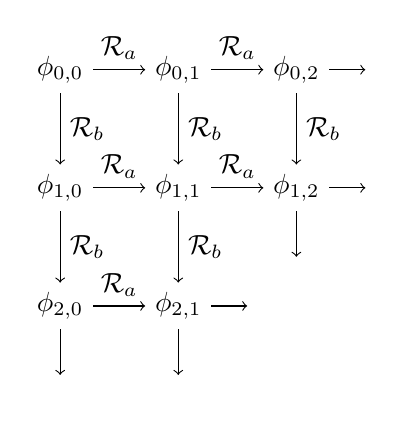
\begin{tikzpicture}[node distance=1.5cm, auto]
  \node (phi00) {$\phi_{0,0}$};
  \node (phi01) [right of=phi00] {$\phi_{0,1}$};
  \node (phi02) [right of=phi01] {$\phi_{0,2}$};
  \node (phi03) [right of=phi02, node distance=1cm] {$ $};

  \node (phi10) [below of=phi00] {$\phi_{1,0}$};
  \node (phi11) [right of=phi10] {$\phi_{1,1}$};
  \node (phi12) [right of=phi11] {$\phi_{1,2}$};
  \node (phi13) [right of=phi12, node distance=1cm] {$ $};

  \node (phi20) [below of=phi10] {$\phi_{2,0}$};
  \node (phi21) [right of=phi20] {$\phi_{2,1}$};
  \node (phi22a) [right of=phi21, node distance=1cm] {$ $};
  \node (phi22b) [below of=phi12, node distance=1cm] {$ $};

  \node (phi30) [below of=phi20, node distance=1cm] {$ $};
  \node (phi31) [below of=phi21, node distance=1cm] {$ $};

  \draw[->] (phi00) to node {$\mathcal{R}_a$} (phi01);
  \draw[->] (phi01) to node {$\mathcal{R}_a$} (phi02);
  \draw[->] (phi02) to node {$ $} (phi03);

  \draw[->] (phi10) to node {$\mathcal{R}_a$} (phi11);
  \draw[->] (phi11) to node {$\mathcal{R}_a$} (phi12);
  \draw[->] (phi12) to node {$ $} (phi13);

  \draw[->] (phi20) to node {$\mathcal{R}_a$} (phi21);
  \draw[->] (phi21) to node {$ $} (phi22a);

  \draw[->] (phi00) to node {$\mathcal{R}_b$} (phi10);
  \draw[->] (phi10) to node {$\mathcal{R}_b$} (phi20);
  \draw[->] (phi20) to node {$ $} (phi30);

  \draw[->] (phi01) to node {$\mathcal{R}_b$} (phi11);
  \draw[->] (phi11) to node {$\mathcal{R}_b$} (phi21);
  \draw[->] (phi21) to node {$ $} (phi31);

  \draw[->] (phi02) to node {$\mathcal{R}_b$} (phi12);
  \draw[->] (phi12) to node {$ $} (phi22b);
\end{tikzpicture}

  \caption{The grid of basis functions $\phi_{k,l}$ for the case $D=2$.}
  \label{fig:phi_kl_grid}
\end{figure}

Every arrow stands for a raising operator $\mathcal{R}$ and we see that there are
two kinds of arrows, vertical and horizontal ones. Following an arrow only one
of the two indices $(k,l)$ changes. This is shown in more details in figure
\ref{fig:phi_kl_operators}.

\begin{figure}[h!]
  \centering
  \subfloat[][]{
    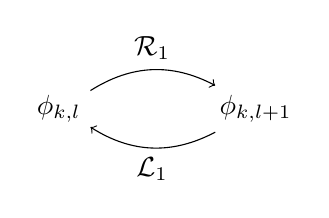
\begin{tikzpicture}[node distance=2.5cm, auto]
  \node (phikl) {$\phi_{k,l}$};
  \node (phikll) [right of=phikl] {$\phi_{k,l+1}$};
  \draw[->] (phikl) to [bend left] node {$\mathcal{R}_1$} (phikll);
  \draw[->] (phikll) to [bend left] node {$\mathcal{L}_1$} (phikl);
\end{tikzpicture}

  }
  \subfloat[][]{
    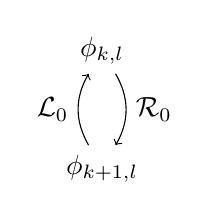
\begin{tikzpicture}[node distance=1.5cm, auto]
  \node (phikl) {$\phi_{k,l}$};
  \node (phikkl) [below of=phikl] {$\phi_{k+1,l}$};
  \draw[->] (phikl) to [bend left] node {$\mathcal{R}_0$} (phikkl);
  \draw[->] (phikkl) to [bend left] node {$\mathcal{L}_0$} (phikl);
\end{tikzpicture}

  } \\
    \caption[]{The two raising and lowering operator pairs in action.}
    \label{fig:phi_kl_operators}
\end{figure}

This fact suggests that we assign a raising operator to each arrow type hence we
get two operators $\mathcal{R}_0$ and $\mathcal{R}_1$ which are of different
nature. We can assign a distinct set $\{\mathcal{R}_i, \mathcal{L}_i\}$ to each
axis $i \in [0, \ldots, D-1]$ of the lattice.

Leaving this introductionary example and following the formal derivation from
\cite{H_ladder_operators} now, we take $\vec{v} \in \mathbb{C}^D$, define
$\vec{y} \assign -i \varepsilon^2 \nabla_x$ and begin with:

\begin{align}
  \mathcal{R}_v & \assign \frac{1}{\sqrt{2\varepsilon^2}}
                  \left(
                    \dotp{-i\mat{P}\vec{\conj{v}}}{(\vec{x}-\vec{q})}
                    -i \dotp{\mat{Q}\vec{\conj{v}}}{(\vec{y}-\vec{p})}
                  \right) \\
                & = \frac{1}{\sqrt{2\varepsilon^2}}
                  \left(
                    i \dotp{\mat{P}\vec{\conj{v}}}{(\vec{x}-\vec{q})}
                    -i \dotp{\mat{Q}\vec{\conj{v}}}{(\vec{y}-\vec{p})}
                  \right) \\
                & = \frac{i}{\sqrt{2\varepsilon^2}}
                  \left(
                    \dotp{\mat{P}\vec{\conj{v}}}{(\vec{x}-\vec{q})}
                    - \dotp{\mat{Q}\vec{\conj{v}}}{(\vec{y}-\vec{p})}
                  \right)
\end{align}

and similarly we get:

\begin{align}
  \mathcal{L}_v & \assign \frac{1}{\sqrt{2\varepsilon^2}}
                  \left(
                    \dotp{\conj{-i \mat{P}}\vec{v}}{(\vec{x}-\vec{q})}
                    +i \dotp{\mat{\conj{Q}}\vec{v}}{(\vec{y}-\vec{p})}
                  \right) \\
                & = \frac{1}{\sqrt{2\varepsilon^2}}
                  \left(
                    -i \dotp{\mat{\conj{P}}\vec{v}}{(\vec{x}-\vec{q})}
                    +i \dotp{\mat{\conj{Q}}\vec{v}}{(\vec{y}-\vec{p})}
                  \right) \\
                & = -\frac{i}{\sqrt{2\varepsilon^2}}
                  \left(
                    \dotp{\mat{\conj{P}}\vec{v}}{(\vec{x}-\vec{q})}
                    - \dotp{\mat{\conj{Q}}\vec{v}}{(\vec{y}-\vec{p})}
                  \right) \,.
\end{align}

For the one-dimensional case we can get back at the definitions from \eqref{eq:raising_ops_1d}.
Following along the lines of \cite{H_ladder_operators} we can compute several commutators:

\begin{align}
  [\mathcal{L}_v, \mathcal{L}_w] & = \mathcal{L}_v\mathcal{L}_w - \mathcal{L}_w\mathcal{L}_v = 0 \\
  [\mathcal{R}_v, \mathcal{R}_w] & = \mathcal{R}_v\mathcal{R}_w - \mathcal{R}_w\mathcal{R}_v = 0 \\
  [\mathcal{L}_v, \mathcal{R}_w] & = \mathcal{L}_v\mathcal{R}_w - \mathcal{R}_w\mathcal{L}_v = \dotp{\vec{v}}{\vec{w}}
\end{align}

for general $\vec{v}, \vec{w} \in \mathbb{C}^D$. The fact that we are allowed to
interchange two raising operators is important and could have been guessed from
figure \ref{fig:phi_kl_grid}. There we have:

\begin{align*}
  \phi_{1,1} & = \mathcal{R}_0 \phi_{0,1} = \mathcal{R}_0 \mathcal{R}_1 \phi_{0,0} \\
  \phi_{1,1} & = \mathcal{R}_1 \phi_{1,0} = \mathcal{R}_1 \mathcal{R}_0 \phi_{0,0}
\end{align*}

thus the order in which we compute $\phi_{k,l}$ from $\phi_{0,0}$ does not matter.
If we flip all arrows we get to the same conclusion but this time for lowering
operators.

From the scalar case we know that we can not simply exchange two different
operators, remember for example the definition of the number operator $\mathcal{N}$.
However, we can go from $\phi_{1,0}$ to $\phi_{0,1}$ by either way:

\begin{align*}
  \phi_{0,1} & = \mathcal{L}_0 \phi_{1,1} = \mathcal{L}_0 \mathcal{R}_1 \phi_{1,0} \\
  \phi_{0,1} & = \mathcal{R}_1 \phi_{0,0} = \mathcal{R}_1 \mathcal{L}_0 \phi_{1,0} \,.
\end{align*}

This is the consequence of the third commutation relation above which tells us
that the two operators commute iff $\vec{v}$ and $\vec{w}$ are orthogonal.

Continuing with the formal derivation we choose a basis of $\mathbb{R}^D$. For
simplicity we take the canonical basis $\{\vec{e}^j\}_{j=0}^{D-1}$. In this basis
we can more precisely say what $\mathcal{R}_v$ is. We define the following two
sets of ladder operators:

\begin{align}
  \mathcal{R}_j & \assign \mathcal{R}_{e^j} \\
  \mathcal{L}_j & \assign \mathcal{L}_{e^j}
\end{align}

each containing exactly $D$ operators. Finally we can build the vector-valued
operators:

\begin{equation} \label{eq:raising_ops_Dd_vectorial}
  \mathcal{R} \assign
  \begin{pmatrix}
    \mathcal{R}_0 \\
    \vdots \\
    \mathcal{R}_{D-1}
  \end{pmatrix}
  \qquad \text{and} \qquad
  \mathcal{L} \assign
  \begin{pmatrix}
    \mathcal{L}_0 \\
    \vdots \\
    \mathcal{L}_{D-1}
  \end{pmatrix} \,.
\end{equation}

Recalling the defining equations for $\mathcal{R}_v$ and $\mathcal{L}_v$ we can
then find explicit expressions for $\mathcal{R}$ and $\mathcal{L}$:

\begin{align} \label{eq:raising_ops_Dd_explicit}
  \mathcal{R} & =  \frac{i}{\sqrt{2\varepsilon^2}} \left( \mat{P}\H (\vec{x}-\vec{q}) - \mat{Q}\H (\vec{y}-\vec{p}) \right) \\
  \mathcal{L} & = -\frac{i}{\sqrt{2\varepsilon^2}} \left( \mat{P}\T (\vec{x}-\vec{q}) - \mat{Q}\T (\vec{y}-\vec{p}) \right) \,.
\end{align}

At this point we should stop for a moment and see what happens if we set $D=1$ now.
If we carried out all calculations we would return step by step to the expressions
given in \eqref{eq:raising_ops_1d}.

With the help of $\mathcal{R}$ we can now go on and define all higher states
$\phi_{\vec{k}}$ properly:

\begin{align} \label{eq:construct_phi_k}
  \phi_{\vec{k}} & \assign \mathcal{R}^{\vec{k}} \phi_{\vec{0}} \\
                 & = \frac{1}{\sqrt{\vec{k}!}} \mathcal{R}_0^{k_0} \mathcal{R}_1^{k_1} \cdots \mathcal{R}_{D-1}^{k_{D-1}} \phi_{\vec{0}} \\
                 & = \frac{1}{\sqrt{\prod_{i=0}^{D-1}k_i!}} \prod_{i=0}^{D-1} \mathcal{R}_i^{k_i} \phi_{\vec{0}} \,.
\end{align}

We can show theorem 3.3 of \cite{H_ladder_operators}:

\begin{theorem}
  The functions $\phi_{\vec{k}}\left[\Pi\right](\vec{x})$ form an orthonormal
  basis of $L^2 \left(\mathbb{R}^D \right)$.
\end{theorem}

For a proof see again this reference.

To close this section we take a closer look at the application of $\mathcal{R}_j$
on $\phi_{\vec{k}}$:

\begin{equation} \label{eq:r_op_applied_1}
  \mathcal{R}_j \phi_{\vec{k}} = \sqrt{k_j + 1} \phi_{\vec{k}^\prime}
\end{equation}

where:

\begin{equation}
  \vec{k}^\prime \assign \vec{k} + \vec{e}^j = (k_0, \ldots, k_{j-1}, k_j+1, k_{j+1}, \ldots, k_{D-1})
\end{equation}

and similarly:

\begin{equation}
  \mathcal{L}_j \phi_{\vec{k}} = \sqrt{k_j} \phi_{\vec{k}^\prime}
\end{equation}

with:

\begin{equation}
  \vec{k}^\prime \assign \vec{k} - \vec{e}^j = (k_0, \ldots, k_{j-1}, k_j-1, k_{j+1}, \ldots, k_{D-1}) \,.
\end{equation}

This justifies the formula \eqref{eq:construct_phi_k} allowing us to construct
$\phi_{\vec{k}}$ out of $\phi_{\vec{0}}$ by raising each index multiple times as
necessary. We build a path through the lattice starting at the origin and ending
at the point $\vec{k}$.

From these formula we see that computing $\mathcal{R} \phi_{\vec{0}}$ is sufficient
to access all higher order functions. The remaining question is how to do this
efficiently. Computing the action of $\mathcal{R}$ is not straight forward because
it contains the differential operator $y \assign -i \varepsilon^2 \nabla_x$. For
this reason we seek a way to compute $\mathcal{R} \phi_{\vec{0}}$ without
ever applying $y$ explicitly. The solution to this task is given by the adjoint
pair $\mathcal{R}, \mathcal{L}$ of operators. We can set up a system of two
operator equations. First we solve the equation defining $\mathcal{L}$ for $y$.
For simplicity of notation we define $\theta \assign \frac{i}{\sqrt{2\varepsilon^2}}$
and transform as follows:

\begin{align} \label{eq:y_op}
  \mathcal{L} & = -\theta \left( \mat{P}\T (\vec{x}-\vec{q}) - \mat{Q}\T (\vec{y}-\vec{p}) \right) \nonumber\\
  \mathcal{L} & = -\theta \mat{P}\T (\vec{x}-\vec{q}) + \theta \mat{Q}\T (\vec{y}-\vec{p}) \nonumber\\
  \mathcal{L} + \theta \mat{P}\T (\vec{x}-\vec{q}) & = \theta \mat{Q}\T (\vec{y}-\vec{p}) \nonumber\\
  \mat{Q}\T (\vec{y}-\vec{p}) & = \frac{1}{\theta} \mathcal{L} + \mat{P}\T (\vec{x}-\vec{q}) \nonumber\\
  \vec{y}-\vec{p} & = \frac{1}{\theta} \mat{Q}\Tinv \mathcal{L} + \mat{Q}\Tinv \mat{P}\T (\vec{x}-\vec{q}) \nonumber\\
  \vec{y} & = \frac{1}{\theta} \mat{Q}\Tinv \mathcal{L} + \mat{Q}\Tinv \mat{P}\T (\vec{x}-\vec{q}) + \vec{p} \,.
\end{align}

Note that solving $\mathcal{R}$ for $y$ gives us the complex conjugate of this
last line:

\begin{equation}  \label{eq:y_op_cc}
  \vec{y} = -\frac{1}{\theta} \mat{Q}\Hinv \mathcal{R} + \mat{Q}\Hinv \mat{P}\H (\vec{x}-\vec{q}) + \vec{p} \,.
\end{equation}

In the next step we plug the result \eqref{eq:y_op} into the definition of
$\mathcal{R}$:

\begin{align} \label{eq:loc_op_r}
  \mathcal{R} & = \theta \left( \mat{P}\H (\vec{x}-\vec{q}) - \mat{Q}\H (\vec{y}-\vec{p}) \right) \nonumber\\
  \mathcal{R} & = \theta \left( \mat{P}\H (\vec{x}-\vec{q}) - \mat{Q}\H \left(\left(
                  \frac{1}{\theta} \mat{Q}\Tinv \mathcal{L} + \mat{Q}\Tinv \mat{P}\T (\vec{x}-\vec{q}) + \vec{p}
                  \right)-\vec{p}\right) \right) \nonumber\\
  \mathcal{R} & = \theta \left( \mat{P}\H (\vec{x}-\vec{q}) - \mat{Q}\H \left(
                  \frac{1}{\theta} \mat{Q}\Tinv \mathcal{L} + \mat{Q}\Tinv \mat{P}\T (\vec{x}-\vec{q})
                  \right) \right) \nonumber\\
  \mathcal{R} & = \theta \left( \mat{P}\H (\vec{x}-\vec{q})
                    - \frac{1}{\theta} \mat{Q}\H\mat{Q}\Tinv \mathcal{L}
                    - \mat{Q}\H\mat{Q}\Tinv\mat{P}\T (\vec{x}-\vec{q})
                  \right) \nonumber\\
  \mathcal{R} & = \theta \left(
                    - \frac{1}{\theta} \mat{Q}\H\mat{Q}\Tinv \mathcal{L}
                    + \underbrace{(\mat{P}\H - \mat{Q}\H\mat{Q}\Tinv\mat{P}\T)}_{*} (\vec{x}-\vec{q})
                  \right) \,.
\end{align}

This is already quite useful a result. But let's see if we can simplify the
underbraced part further. Simplifying the $*$ part needs a bit of algebra. We
start with the basic relations in \eqref{eq:PQcond_Dd} and multiply the first
one by $\mat{Q}\inv$ from the right:

\begin{align*}
  \mat{Q}\H \mat{P} - \mat{P}\H \mat{Q} & = 2i \id \\
  \mat{Q}\H \mat{P} \mat{Q}\inv - \mat{P}\H \mat{Q} \mat{Q}\inv & = 2i \mat{Q}\inv \\
  \mat{Q}\H \mat{P} \mat{Q}\inv - \mat{P}\H & = 2i \mat{Q}\inv \\
  \mat{P}\H - \mat{Q}\H \underbrace{\mat{P} \mat{Q}\inv}_{**} & = -2i \mat{Q}\inv \,.
\end{align*}

Now we are left with $**$ where we can apply the other fundamental relation which
we have to transform a little bit first:

\begin{align*}
  \mat{P}\T \mat{Q} - \mat{Q}\T \mat{P} & = \mat{0} \\
  \mat{Q}\Tinv \mat{P}\T \mat{Q} - \mat{Q}\Tinv \mat{Q}\T \mat{P} & = \mat{0} \\
  \mat{Q}\Tinv \mat{P}\T \mat{Q} & = \mat{P} \,.
\end{align*}

The last line can now be used to replace the $\mat{P}$ in $**$ which yields:

\begin{align*}
  \mat{P}\H - \mat{Q}\H \mat{Q}\Tinv \mat{P}\T \mat{Q} \mat{Q}\inv & = -2i \mat{Q}\inv \\
  \mat{P}\H - \mat{Q}\H \mat{Q}\Tinv \mat{P}\T & = -2i \mat{Q}\inv \,.
\end{align*}

This is the part $*$ we wanted to simplify. Going back to \eqref{eq:loc_op_r}
we can write:

\begin{align*}
  \mathcal{R} & = \theta \left(
                    - \frac{1}{\theta} \mat{Q}\H\mat{Q}\Tinv \mathcal{L}
                    -2i \mat{Q}\inv (\vec{x}-\vec{q})
                  \right) \\
  \mathcal{R} & = - \mat{Q}\H\mat{Q}\Tinv \mathcal{L}
                    -2i \theta \mat{Q}\inv (\vec{x}-\vec{q}) \,.
\end{align*}

At the end of the day we get:

\begin{equation} \label{eq:r_op_wo_deriv}
  \boxed{
    \mathcal{R} = \sqrt{\frac{2}{\varepsilon^2}} \mat{Q}\inv (\vec{x}-\vec{q}) - \mat{Q}\H\mat{Q}\Tinv \mathcal{L}
  }
\end{equation}

where we reinserted the term for $\theta$ and took into account the $i$ therein.
Of course we would get the very same result if we used \eqref{eq:y_op_cc} and
plugged it into the definition of $\mathcal{L}$. Just for the sake of completeness
we state the complex conjugate result for the $\mathcal{L}$ operator too:

\begin{equation}
  \boxed{
    \mathcal{L} = \sqrt{\frac{2}{\varepsilon^2}} \mat{\conj{Q}}\inv (\vec{x}-\vec{q}) - \mat{Q}\T\mat{Q}\Hinv \mathcal{R}
  }
\end{equation}

with a similar derivation as the one above.


\section{Higher order basis functions}


With this equation at hand we can continue in \eqref{eq:r_op_applied_1} where we
left off computing $\mathcal{R}_d \phi_{\vec{k}}$. We start applying the operator
for the $d$-th direction. But we do not have an explicit expression for
$\mathcal{R}_d$ and on the other hand we need the result for all $d \in [0, \ldots, D-1]$.
Therefore is seems wise to do these computations simultaneously for all $D$ components:

\begin{align}
  \begin{pmatrix}
    \sqrt{k_0 + 1} \phi_{\vec{k}+\vec{e}^0} \\
    \vdots \\
    \sqrt{k_{D-1} + 1} \phi_{\vec{k}+\vec{e}^{D-1}}
  \end{pmatrix}
  =
  \begin{pmatrix}
    \mathcal{R}_0 \phi_{\vec{k}} \\
    \vdots \\
    \mathcal{R}_{D-1} \phi_{\vec{k}}
  \end{pmatrix}
  =
  \mathcal{R} \phi_{\vec{k}}
\end{align}

Using the formula \eqref{eq:r_op_wo_deriv} for $\mathcal{R}$ gives us:

\begin{equation} \label{eq:basis_recursion_DD}
  \begin{pmatrix}
    \sqrt{k_0+1} \, \phi_{\vec{k}+\vec{e}^0} \\
    \vdots \\
    \sqrt{k_{D-1}+1} \, \phi_{\vec{k}+\vec{e}^{D-1}}
  \end{pmatrix}
  =
  \sqrt{\frac{2}{\varepsilon^2}} \mat{Q}\inv (\vec{x}-\vec{q}) \phi_{\vec{k}}
  - \mat{Q}\H\mat{Q}\Tinv
  \begin{pmatrix}
    \sqrt{k_0} \phi_{\vec{k}-\vec{e}^0} \\
    \vdots \\
    \sqrt{k_{D-1}} \phi_{\vec{k}-\vec{e}^{D-1}}
  \end{pmatrix} \,.
\end{equation}

From this we get the new functions $\phi_{\vec{k}+\vec{e}^d}$ as:

\begin{equation*}
  \begin{pmatrix}
    \phi_{\vec{k}+\vec{e}^0} \\
    \vdots \\
    \phi_{\vec{k}+\vec{e}^{D-1}}
  \end{pmatrix}
  = \left(
  \sqrt{\frac{2}{\varepsilon^2}} \mat{Q}\inv (\vec{x}-\vec{q}) \phi_{\vec{k}}
  - \mat{Q}\H\mat{Q}\Tinv
  \begin{pmatrix}
    \sqrt{k_0} \phi_{\vec{k}-\vec{e}^0} \\
    \vdots \\
    \sqrt{k_{D-1}} \phi_{\vec{k}-\vec{e}^{D-1}}
  \end{pmatrix}
  \right)
  \oslash
  \begin{pmatrix}
    \sqrt{k_0+1}\\
    \vdots \\
    \sqrt{k_{D-1}+1}
  \end{pmatrix}
\end{equation*}

where the operator $\oslash$ denotes component-wise division. In a next step
we use this formula for evaluation of all $\phi_{\vec{k}}$ basis functions
of $D$ dimensional semi-classical wavepackets. This last formula is so important
that it should carry a box too but it seems there is no space left.


\begin{figure}
  \centering
  \subfloat[][]{
    \label{fig:phi_00}
    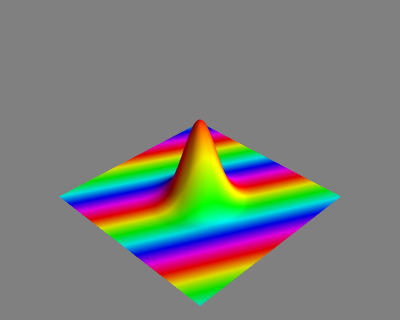
\includegraphics[width=0.5\linewidth]{./fig/phi/phi_0-0.png}
  }
  \subfloat[][]{
    \label{fig:phi_10}
    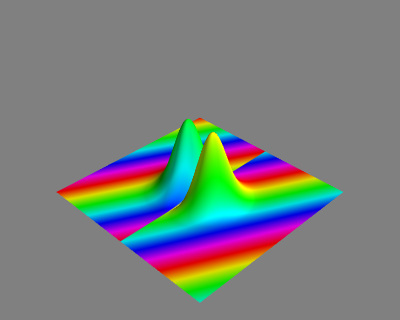
\includegraphics[width=0.5\linewidth]{./fig/phi/phi_1-0.png}
  } \\
  \subfloat[][]{
    \label{fig:phi_01}
    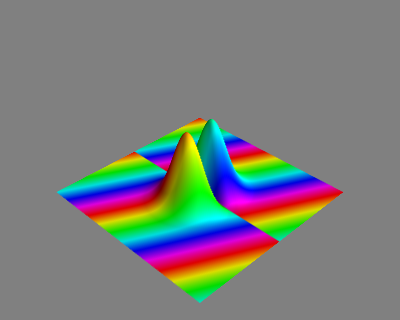
\includegraphics[width=0.5\linewidth]{./fig/phi/phi_0-1.png}
  }
  \subfloat[][]{
    \label{fig:phi_11}
    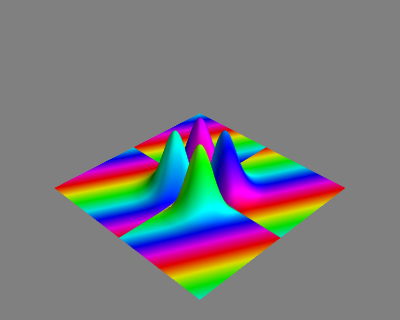
\includegraphics[width=0.5\linewidth]{./fig/phi/phi_1-1.png}
  } \\
  \subfloat[][]{
    \label{fig:phi_02}
    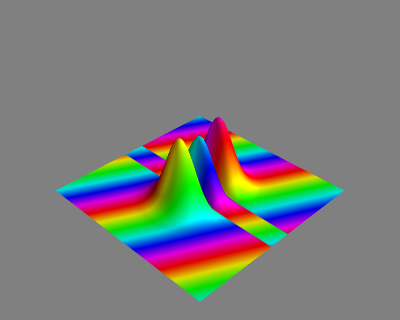
\includegraphics[width=0.5\linewidth]{./fig/phi/phi_0-2.png}
  }
  \subfloat[][]{
    \label{fig:phi_12}
    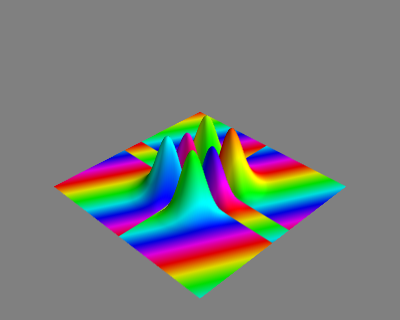
\includegraphics[width=0.5\linewidth]{./fig/phi/phi_1-2.png}
  } \\
  \caption[Plots of some basis functions $\phi$]{
    Plots of the first few functions $\phi_{k,l}$ with parameters set
    to $\vec{q} = \vec{0}$, $\vec{p} = (1, \frac{1}{2})$, $\mat{Q} = \id$, $\mat{P} = i \id$
    and $\varepsilon = 1$. The surface represents ten times the value
    $\sqrt{\Braket{\phi_{k,l}|\phi_{k,l}}}$ where the factor of $10$
    is just for visual purpose. For an explanation of the colours, see appendix \ref{ch:color_code}.
    \subref{fig:phi_00} $\phi_{0,0}$
    \subref{fig:phi_10} $\phi_{1,0}$
    \subref{fig:phi_01} $\phi_{0,1}$
    \subref{fig:phi_11} $\phi_{1,1}$
    \subref{fig:phi_02} $\phi_{0,2}$
    \subref{fig:phi_12} $\phi_{1,2}$
    \label{fig:phi_table_1}
  }
\end{figure}


\begin{figure}
  \centering
  \subfloat[][]{
    \label{fig:phi_20}
    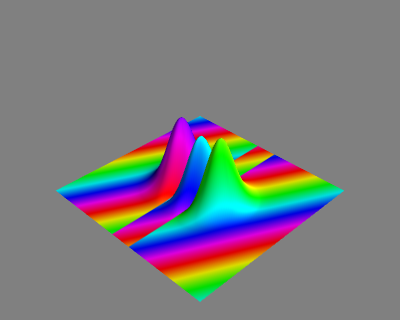
\includegraphics[width=0.5\linewidth]{./fig/phi/phi_2-0.png}
  }
  \subfloat[][]{
    \label{fig:phi_30}
    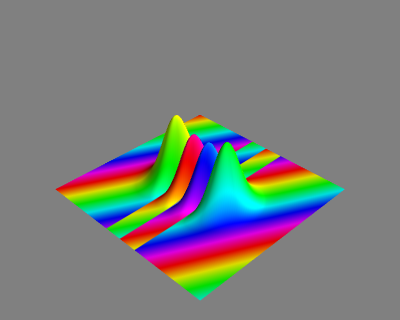
\includegraphics[width=0.5\linewidth]{./fig/phi/phi_3-0.png}
  } \\
  \subfloat[][]{
    \label{fig:phi_21}
    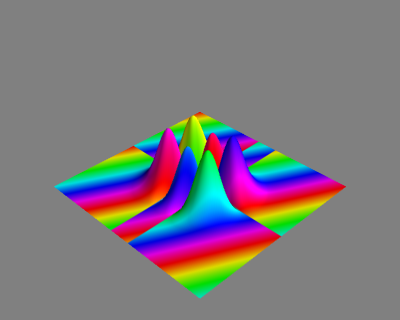
\includegraphics[width=0.5\linewidth]{./fig/phi/phi_2-1.png}
  }
  \subfloat[][]{
    \label{fig:phi_31}
    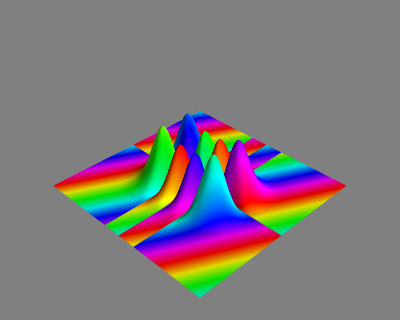
\includegraphics[width=0.5\linewidth]{./fig/phi/phi_3-1.png}
  } \\
  \subfloat[][]{
    \label{fig:phi_22}
    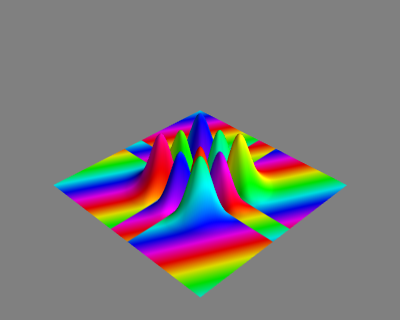
\includegraphics[width=0.5\linewidth]{./fig/phi/phi_2-2.png}
  }
  \subfloat[][]{
    \label{fig:phi_32}
    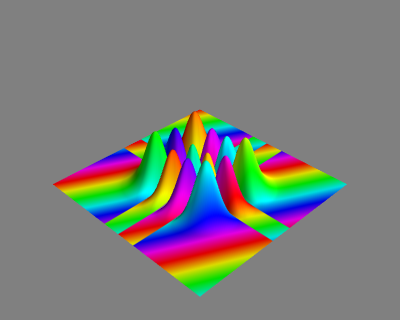
\includegraphics[width=0.5\linewidth]{./fig/phi/phi_3-2.png}
  } \\
  \caption[Plots of some basis functions $\phi$]{
    Plots of the first few functions $\phi_{k,l}$ with parameters set
    to $\vec{q} = \vec{0}$, $\vec{p} = (1, \frac{1}{2})$, $\mat{Q} = \id$, $\mat{P} = i \id$
    and $\varepsilon = 1$. The surface represents ten times the value
    $\sqrt{\Braket{\phi_{k,l}|\phi_{k,l}}}$ where the factor of $10$
    is just for visual purpose. For an explanation of the colours, see appendix \ref{ch:color_code}.
    \subref{fig:phi_20} $\phi_{2,0}$
    \subref{fig:phi_30} $\phi_{3,0}$
    \subref{fig:phi_21} $\phi_{2,1}$
    \subref{fig:phi_31} $\phi_{3,1}$
    \subref{fig:phi_22} $\phi_{2,2}$
    \subref{fig:phi_32} $\phi_{3,2}$
    \label{fig:phi_table_2}
  }
\end{figure}


\section{Construction of wavepackets}


In the previous section we saw how to compute the functions $\phi_{\vec{k}}[\Pi](\vec{x})$.
Now we can take a very general set $\mathfrak{K}$ of indices $\vec{k}$ and use
the corresponding functions $\phi_{\vec{k}}$ to build a (more or less truncated)
basis for $L^2(\mathbb{R}^D)$. In a first step we can construct so called
\emph{scalar wavepackets} $\Phi$ by linear combinations:

\begin{equation}
  \Phi(\vec{x}) \assign \exp\left(\frac{i S}{\varepsilon^2}\right) \sum_{\vec{k}\in\mathfrak{K}} c_{\vec{k}} \phi_{\vec{k}}
\end{equation}

where the coefficients $c_{\vec{k}} \in \mathbb{C}$ depend on time only and the basis functions
$\phi_{\vec{k}}$ depend on space but also on time through the parameter set
$\Pi(t)$ which is time-dependent\footnote{In general we neglect explicit
time-dependence of the parameter set $\Pi$ in our notation.}. We added a global
phase $S$ which is also time-dependent. An overly precise notation reads:

\begin{definition}[Scalar semi-classical wavepacket]
  \begin{equation} \label{eq:scalar_wavepacket}
    \Ket{\Phi} \assign
    \Phi\left[\Pi(t)\right](\vec{x}, t)
    =
    \exp\left(\frac{i S(t)}{\varepsilon^2}\right) \sum_{\vec{k}\in\mathfrak{K}} c_{\vec{k}}(t) \phi_{\vec{k}}\left[\Pi(t)\right](\vec{x}) \,.
  \end{equation}
\end{definition}

Every single basis function $\phi_{\vec{k}}$ is a perfectly valid wavepacket too.
Sometimes we will append the parameter $S$ to the set $\Pi$ and use the notation
$\Pi = \{q,p,Q,P,S\}$. This should be clear from the context. Also we will drop
the time variable since we look at wavepackets at fixed times.


\section{Basis set expansion and basis shapes}


The above formulation is a basis expansion for the true wavefunction $\varphi(\vec{x}, t)$.
Remember that the set $\{\phi_{\vec{k}}\}_{\vec{k}\in\mathfrak{K}}$ is a (complete)
basis of the function space $L^2(\mathbb{R}^D)$. Hence the basis expansion is
exact if we take the full lattice $\mathfrak{K} = \mathbb{N}_0^D$ of indices. In
theoretical considerations we can use the full lattice but for all practical
purposes we need to truncate the basis and make the set $\mathfrak{K}$ finite.
This can be done in various ways and we refer to the \emph{shape} of a basis set
if we speak about these details of $\mathfrak{K}$. Basis shapes usually depend
on some parameters $\theta$, we occasionally write $\mathfrak{K}(\theta)$ for this.

For a first ansatz we can use a hypercubic basis set $\mathfrak{K}$ which means
that we take the subset of all lattice points for which $\vec{k} < \vec{K}$ holds.
The components of $\vec{K}$ specify the number of points along each of the $D$
directions. A more formal definition is:

\begin{definition}[Hypercubic basis shape]
  \begin{equation}
    \mathfrak{K}(\vec{K}) \assign \left\{ \vec{k} \in \mathbb{N}_0^D :
                                          \, k_d < K_d \,\forall\, d \in [0, \ldots, D-1] \right\} \,.
  \end{equation}
\end{definition}

If we use this basis shape we call the resulting wavepacket \emph{dense}. By
$|\mathfrak{K}|$ we denote the \emph{basis size}, the overall number of basis
functions $\phi_{\vec{k}}$ we use. In the hypercubic case this is obviously:

\begin{equation}
  |\mathfrak{K}| = \prod_{d=0}^{D-1} K_d \,.
\end{equation}

As a shorthand notation to specify the hypercubic shape we simply write
$\mathfrak{K} = \vec{K} = [K_0, \ldots, K_{D-1}]$. We should think of $\vec{K}$ as
being both the vector in the lattice $\mathbb{N}_0^D$ and the set of all index
points in the hypercube spanned by the origin $\vec{0} = (0, \ldots, 0)$ and
$\vec{K} - \vec{1} = (K_0-1, \ldots, K_{D-1}-1)$, depending on the context.

The size of this basis shape grows exponentially with the number $D$ of dimensions.
Therefore we introduce more sparse basis sets which grow slower as the number
of dimensions increases. The first example is the \emph{hyperbolic cut} basis shape
defined as follows:

\begin{definition}[Hyperbolic cut basis shape] \label{def:hyperbolic_cut_shape}
  \begin{equation}
    \mathfrak{K}(K) \assign \left\{ \vec{k} \in \mathbb{N}_0^D :
                                    \, \prod_{d=0}^{D-1}(1+k_d) \leq K \right\}
  \end{equation}
\end{definition}

where we limit the number of basis functions by hyperbolic cuts. For this we
introduce a scalar parameter $K \in \mathbb{N}$ which we call \emph{sparsity}
in this context. The number of basis functions is then bounded by:

\begin{equation}
  |\mathfrak{K}| \leq \mathcal{C} K \left(\log K\right)^{D-1} \,.
\end{equation}

where $\mathcal{C}$ is some constant.

Figure \ref{fig:hyperbolic_cut_basis_size} shows the application of this bound
to the two-dimensional case.

\begin{figure}
  \centering
  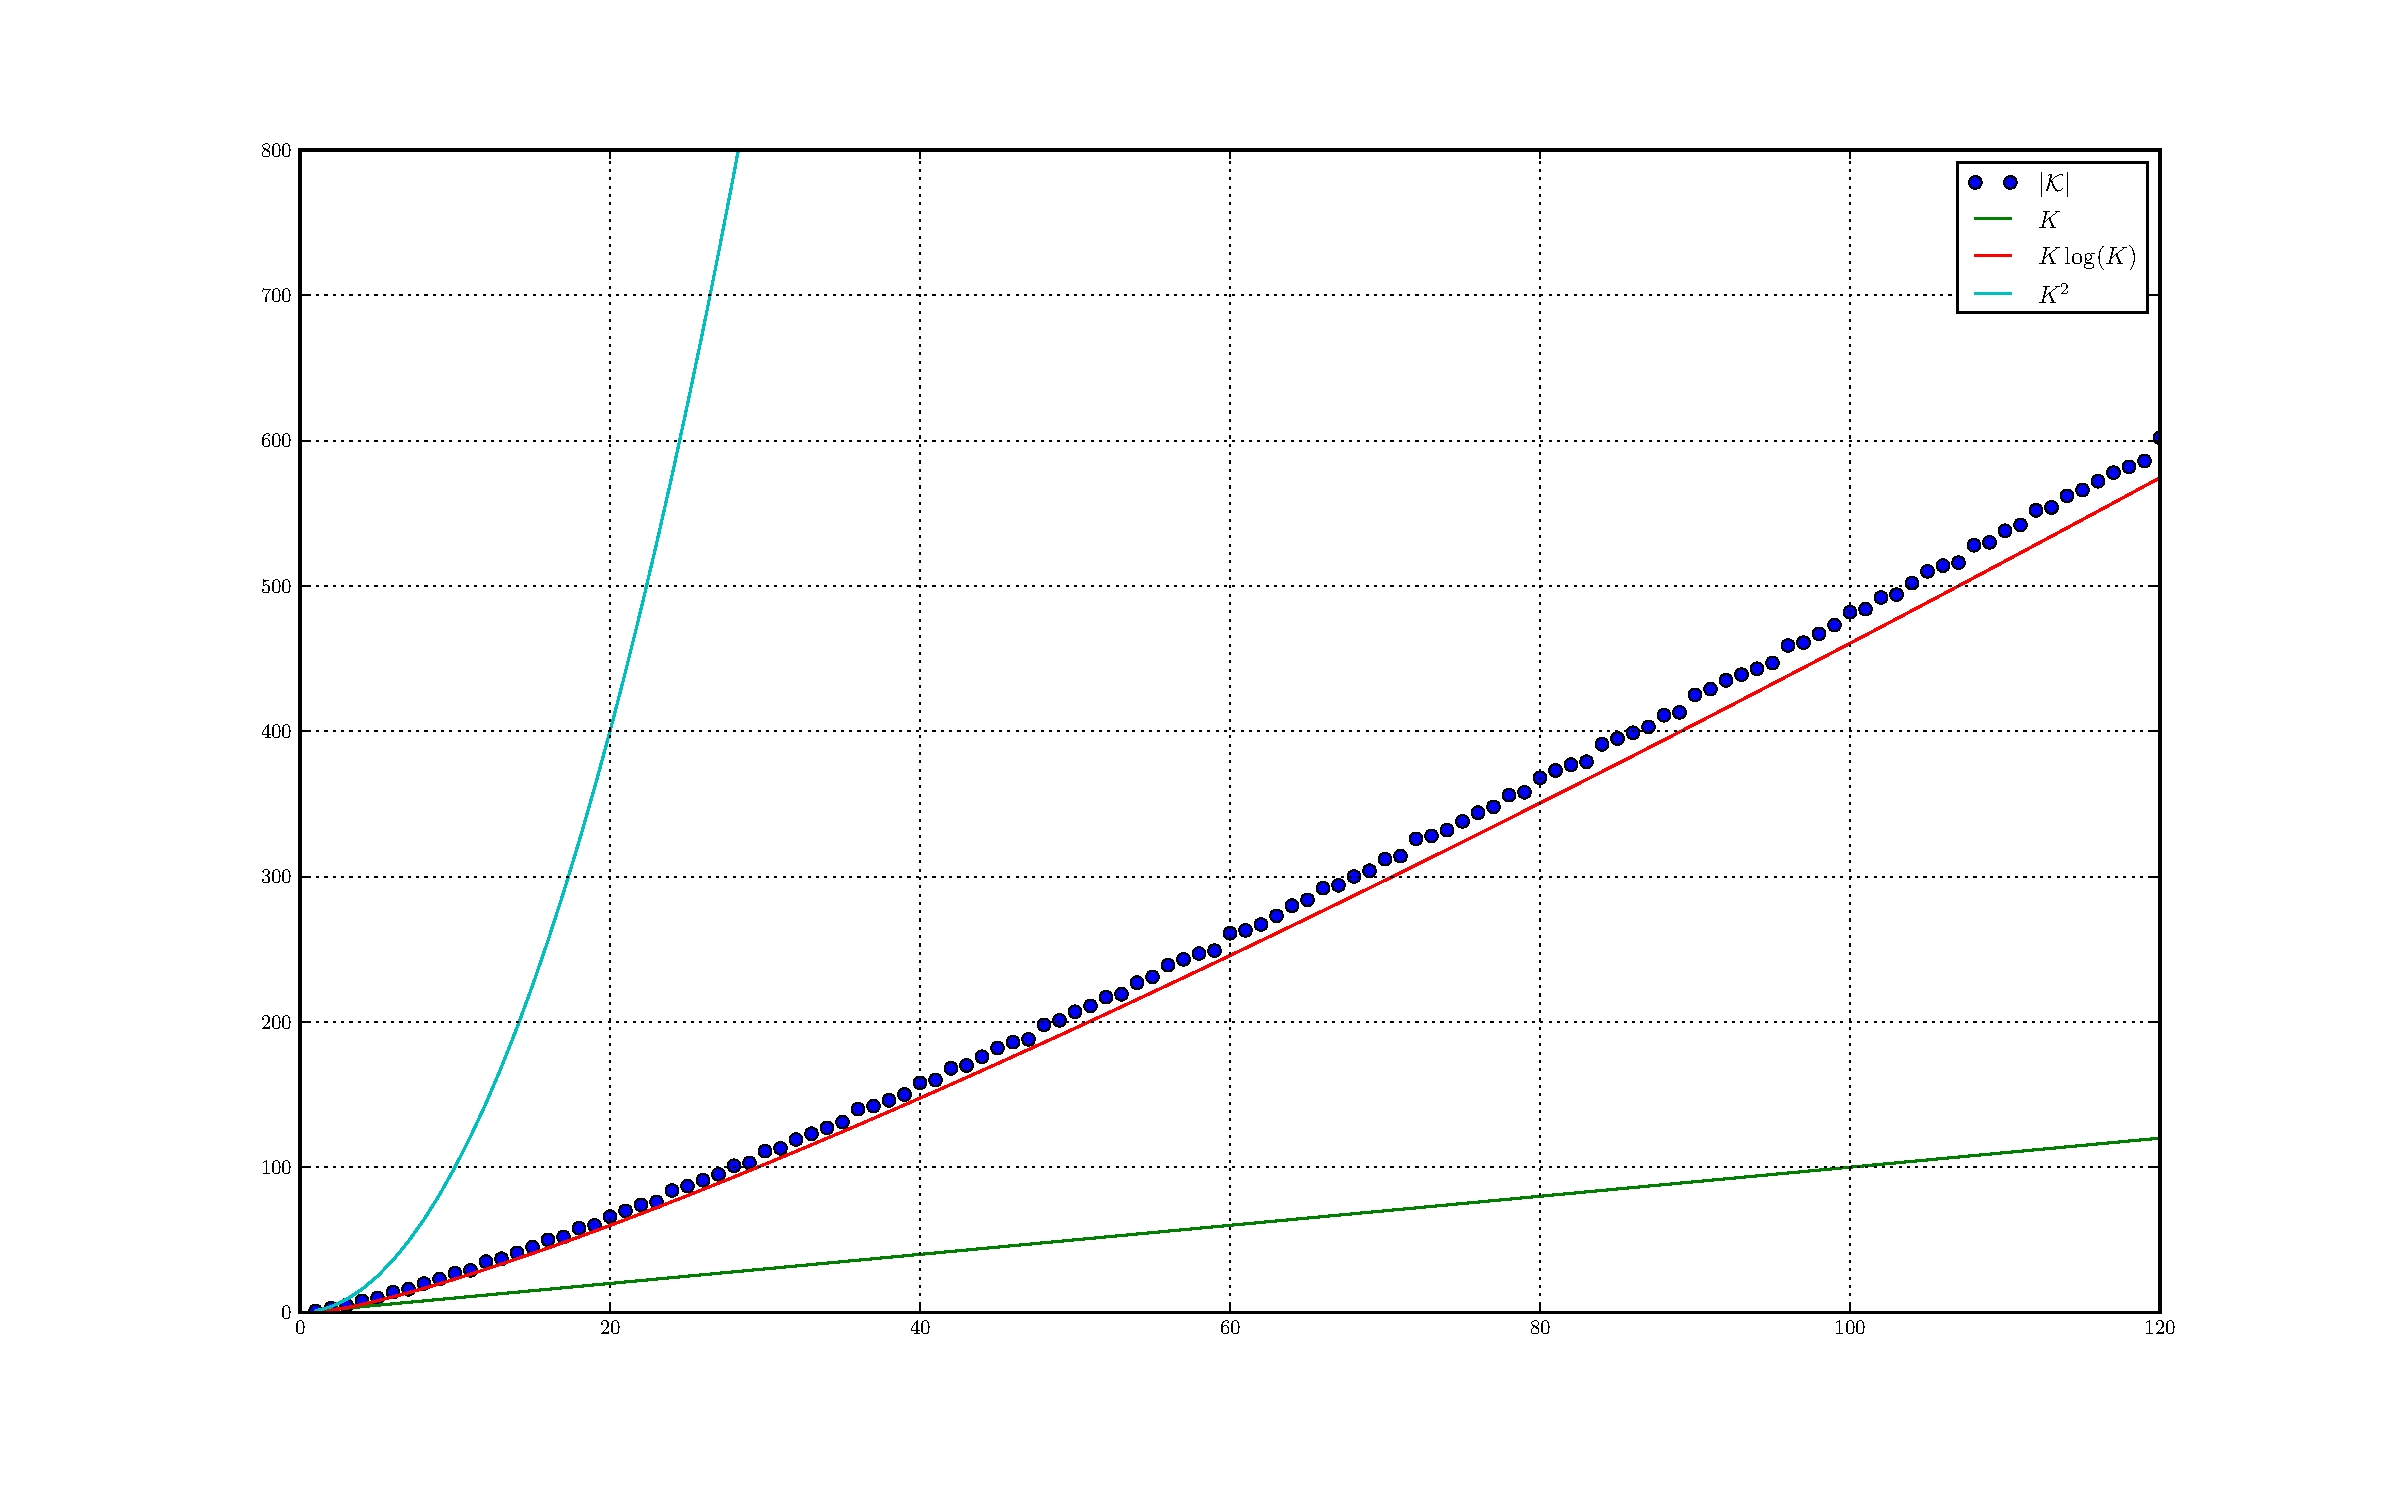
\includegraphics[width=0.8\linewidth]{./fig/basis_size.pdf}
  \caption{The size $|\mathfrak{K}|$ of two-dimensional hyperbolic basis shapes
           with various cut-off values $K$.}
  \label{fig:hyperbolic_cut_basis_size}
\end{figure}

\begin{figure}
  \centering
  \subfloat[][]{
    \label{fig:hyperbolic_cut_2_8}
    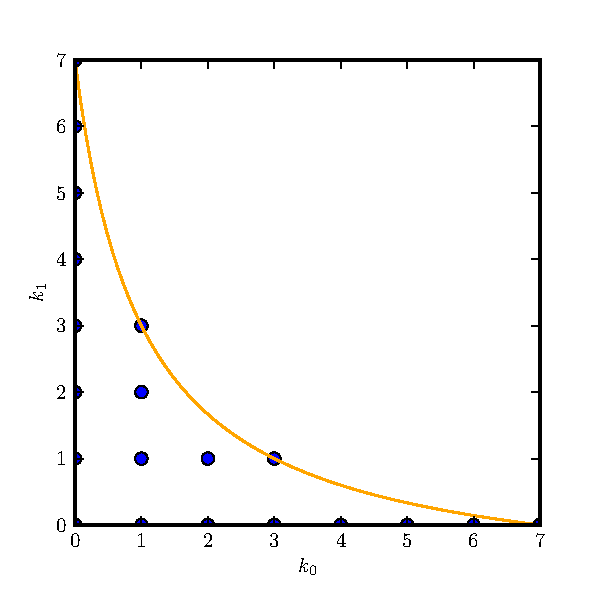
\includegraphics[width=0.5\linewidth]{./fig/hyperbolic_shape_2_8.pdf}
  }
  \subfloat[][]{
    \label{fig:hyperbolic_cut_2_32}
    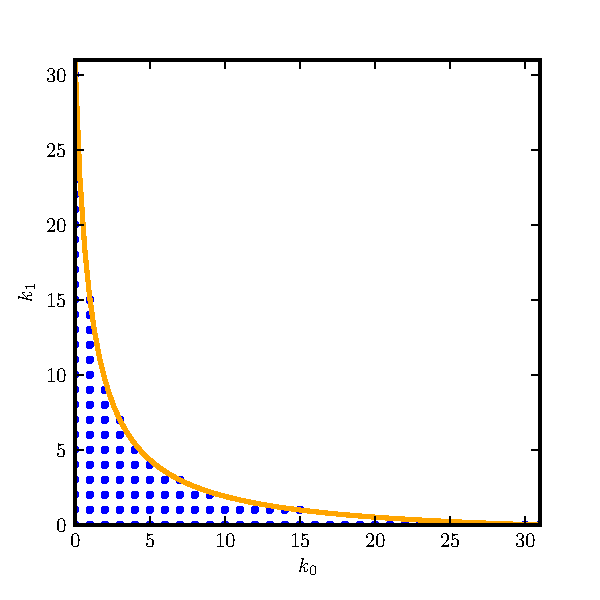
\includegraphics[width=0.5\linewidth]{./fig/hyperbolic_shape_2_32.pdf}
  } \\
  \caption[Hyperbolic cut basis shape in two dimensions]{
    The lattice nodes that are part of a two-dimensional hyperbolic cut basis
    shape. Additionally the cut-off function is shown. Compared to the full
    hypercubic basis shape the sparsity of this type of basis shape becomes
    clearly visible.
    \subref{fig:hyperbolic_cut_2_8} $K = 8$
    \subref{fig:hyperbolic_cut_2_32} $K = 32$
    \label{fig:hyperbolic_cut_2D}
  }
\end{figure}

\begin{figure}
  \centering
  \subfloat[][]{
    \label{fig:hyperbolic_cut_3_8}
    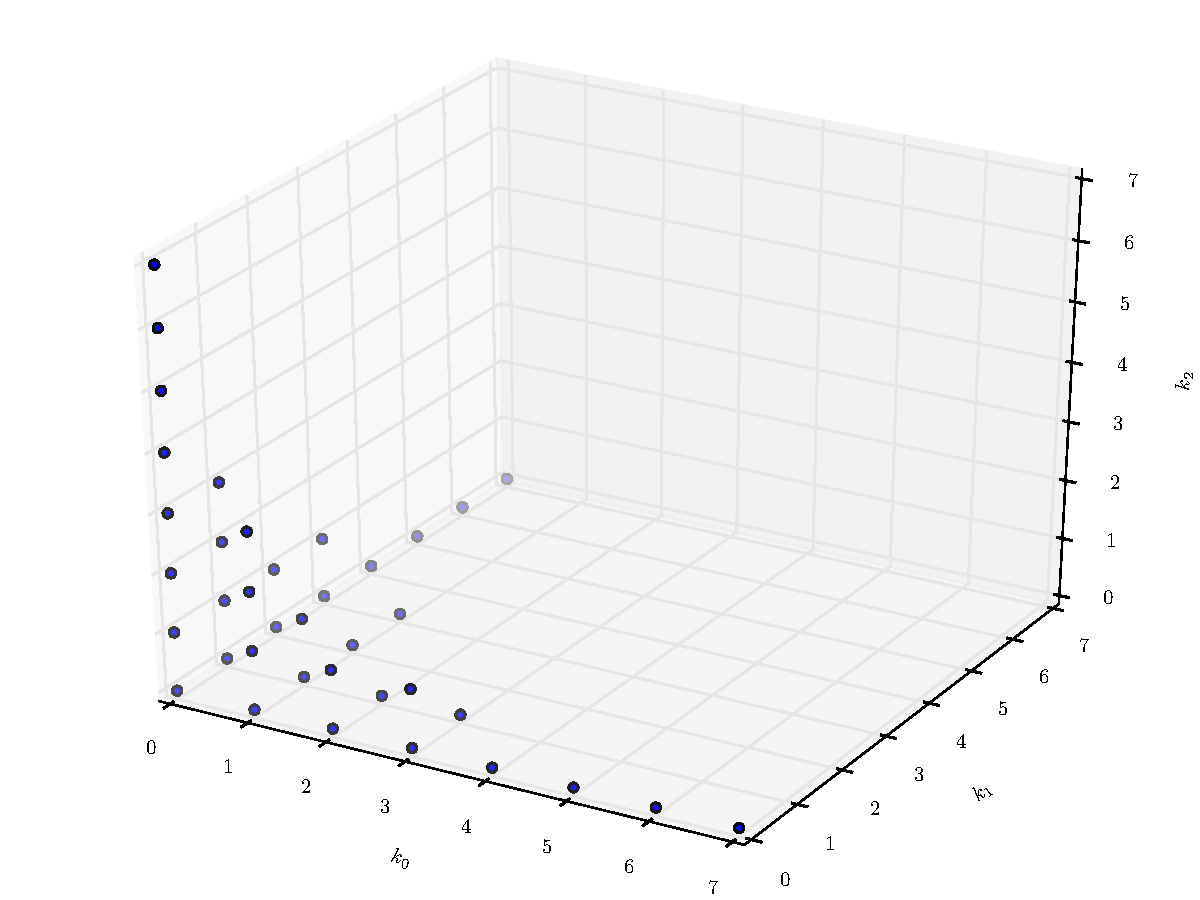
\includegraphics[width=0.5\linewidth]{./fig/hyperbolic_shape_3_8.pdf}
  }
  \subfloat[][]{
    \label{fig:hyperbolic_cut_3_32}
    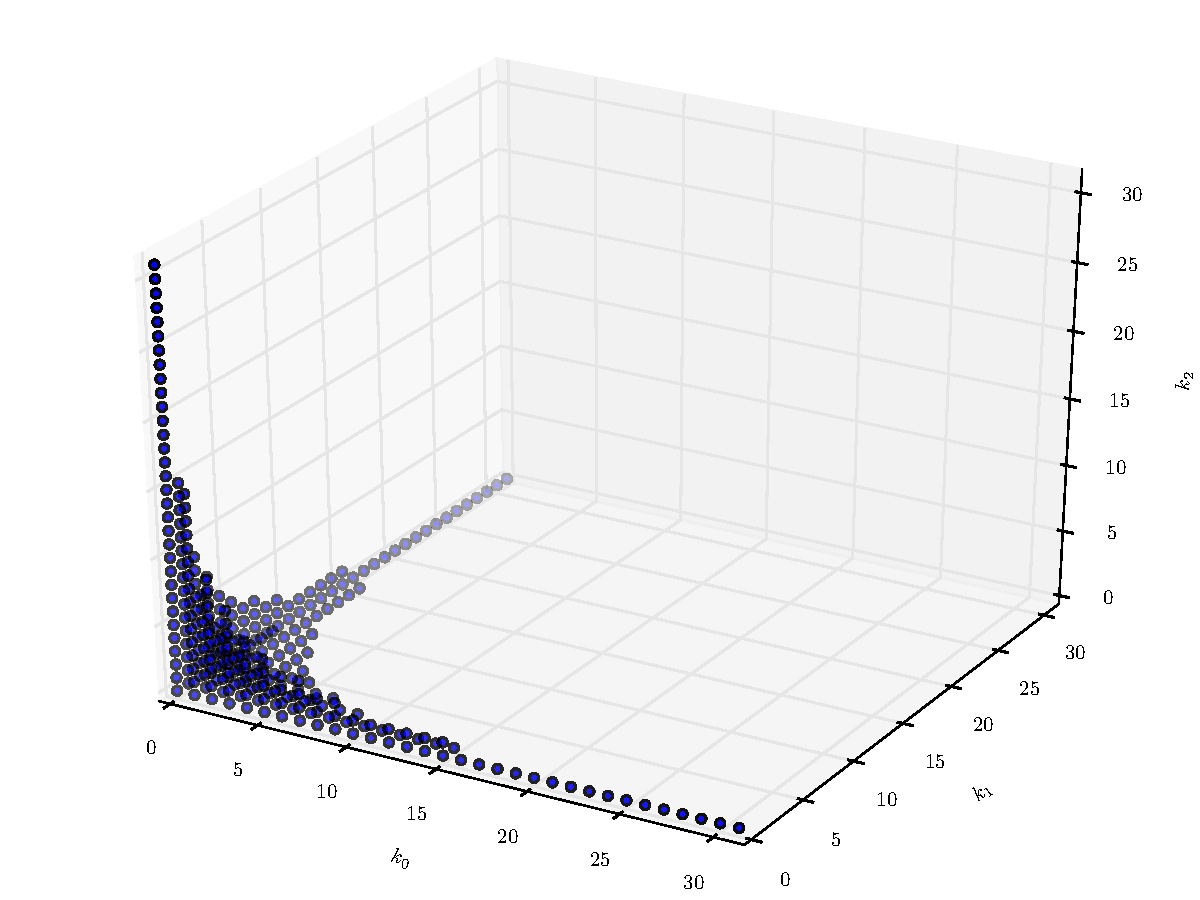
\includegraphics[width=0.5\linewidth]{./fig/hyperbolic_shape_3_32.pdf}
  } \\
  \caption[Hyperbolic cut basis shape in three dimensions]{
    The lattice nodes that are part of a three-dimensional hyperbolic cut basis
    shape. Compared to the full hypercubic basis shape the sparsity of this
    type of basis shape becomes clearly visible.
    \subref{fig:hyperbolic_cut_3_8} $K = 8$
    \subref{fig:hyperbolic_cut_3_32} $K = 32$
    \label{fig:hyperbolic_cut_3D}
  }
\end{figure}

As we see in figures \ref{fig:hyperbolic_cut_2D} and \ref{fig:hyperbolic_cut_3D}
this basis shape has long tails consisting of functions with high frequencies
in one direction. Sometimes we do not need these tails. We can combine the two
basis shapes introduced and define a new shape:

\begin{definition}[Hyperbolic cut basis shape with limits]
  \begin{equation}
    \mathfrak{K}(K, \vec{L}) \assign \left\{ \vec{k} \in \mathbb{N}_0^D :
                             \prod_{d=0}^{D-1}(1+k_d) \leq K
                             \land k_d < L_d \,\forall\, d \in [0,\ldots,D-1] \right\} \,.
  \end{equation}
\end{definition}

The parameter $K \in \mathbb{N}$ is again the sparsity defining the hyperbolic
cuts. The parameter $\vec{L}$ is a list of $D$ elements with each $L_d \in \mathbb{N}$.
These limits act as sharp upper bounds on the entries of $\vec{k}$. In that way
we can combine the two previous basis shapes. If we choose $L_d \geq K \,\forall\,
d \in [0,\ldots, D-1]$ then we obtain a simple hyperbolic cut basis shape. On the
other hand, if we set $K \geq \prod_{d=0}^{D-1} L_d$ we are back in the full
hypercubic case.

\begin{figure}
  \centering
  \subfloat[][]{
    \label{fig:hyperbolic_limited_2_8}
    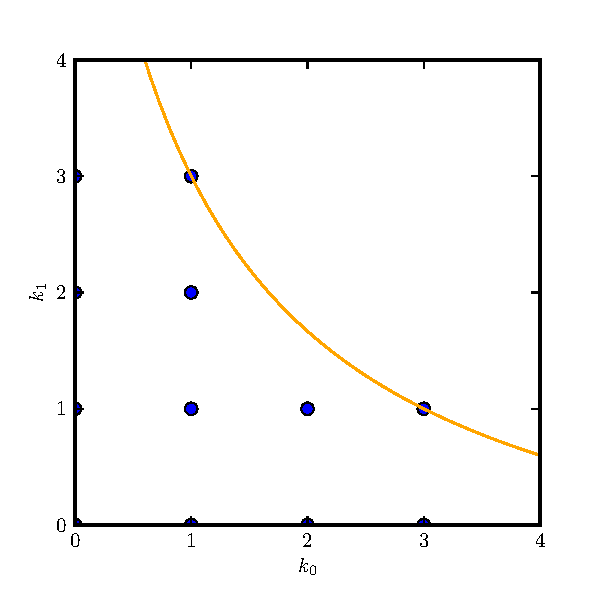
\includegraphics[width=0.5\linewidth]{./fig/hyperbolic_limited_2_8.pdf}
  }
  \subfloat[][]{
    \label{fig:hyperbolic_limited_2_32}
    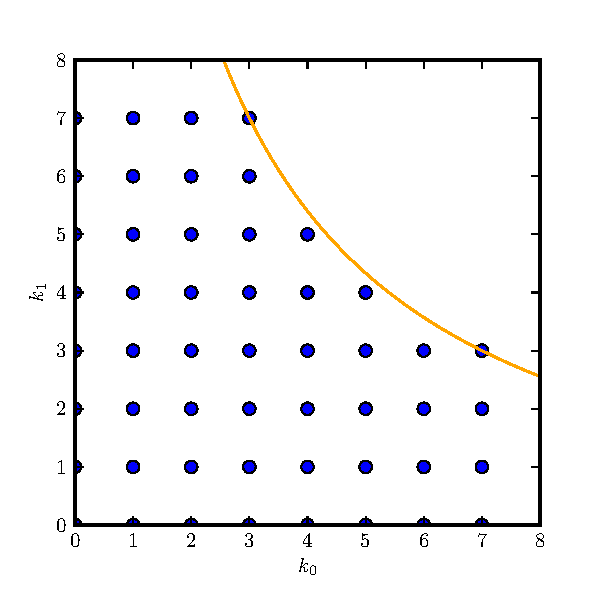
\includegraphics[width=0.5\linewidth]{./fig/hyperbolic_limited_2_32.pdf}
  } \\
  \caption[Hyperbolic cut basis shape with limits in two dimensions]{
    The lattice nodes that are part of a two-dimensional limited hyperbolic cut
    basis shape. Compared to the unlimited hyperbolic cut basis shape
    the long tails are missing here.
    \subref{fig:hyperbolic_limited_2_8} $K = 8$ and $\vec{L} = (4,4)$
    \subref{fig:hyperbolic_limited_2_32} $K = 32$ and $\vec{L} = (8,8)$
    \label{fig:hyperbolic_limited_2D}
  }
\end{figure}

There exist many more possibilities for specific basis shapes. For a generic
basis shape $\mathfrak{K}$ a fundamental property has to hold. We can state
it by the following implication:

\begin{equation}
  \forall\, \vec{k} \in \mathbb{N}_0^D:
  \vec{k} \in \mathfrak{K} \Rightarrow \vec{k} - \vec{e}^d \in \mathfrak{K} \,\forall\, d \in [0, \ldots, D-1] \,.
\end{equation}

% \begin{equation}
%   \mathfrak{K} := \left\{ \vec{k} \in \mathbb{N}_0^D :
%                           \vec{k} - \vec{e}^d \in \mathfrak{K} \,\forall\, d \in [0, \ldots, D-1] \right\} \,.
% \end{equation}

In other words, for each $\vec{k} \in \mathfrak{K}$ it must hold that for all
$d = 0, \ldots, D-1$ the multi-index defined by $k^\prime \assign \vec{k} - \vec{e}^d$
has no negative components and $\vec{k}^\prime \in \mathfrak{K}$. In less formal
terms this means that an index $\vec{k}$ is part of $\mathfrak{K}$ iff all its
backward neighbours are also part of $\mathfrak{K}$. This condition is necessary
for the recursive evaluation of wavepackets which we will show later.

Probably the most general way to write a scalar wavepacket \eqref{eq:scalar_wavepacket}
now is:

\begin{equation}
  \Ket{\Phi} \assign
  \Phi\left[\Pi(t), \mathfrak{K}(t)\right](\vec{x}, t)
  =
  \exp\left(\frac{i S(t)}{\varepsilon^2}\right) \sum_{\vec{k}\in\mathfrak{K}(t)} c_{\vec{k}}(t) \phi_{\vec{k}}\left[\Pi(t)\right](\vec{x})
\end{equation}

which uses an arbitrary, possibly time-adaptive basis shape $\mathfrak{K}(t)$. In
principle we can exchange the basis shapes at each timestep during the simulation.
This provides us with adaptivity for all parameters $\theta$ a basis shape depends on.

Sometimes we will need to bring the elements $\vec{k}$ of a basis shape $\mathfrak{K}$
into a fixed total order. This is done by the \emph{linearisation mapping}.

\begin{definition}[Linearisation mapping]
  A mapping:
  \begin{align*}
    \mu : \mathfrak{K} & \rightarrow \mathbb{N}_0 \\
          \vec{k}      & \mapsto     n
  \end{align*}
  that fixes a total order of the set $\mathfrak{K}$.
\end{definition}

If it is not clear from the context we denote this mapping by $\mu_{\mathfrak{K}}$
to mark explicitly which basis shape it belongs to. In practical cases we usually
have $\mu(\vec{0}) = 0$ but this is not a requirement.

Finally the following two algorithms \ref{al:forward_neighbours} and
\ref{al:backward_neighbours} can be used to find the neighbourhood
of a given multi-index $\vec{k}$ in a general basis shape $\mathfrak{K}$.

\begin{algorithm}
  \caption{Find forward neighbours}
  \label{al:forward_neighbours}
  \begin{algorithmic}
    \REQUIRE The number $D$ of space dimensions
    \REQUIRE The basis shape $\mathfrak{K}$
    \REQUIRE The multi-index $\vec{k}$ whose neighbours we search

    \STATE // List for the result
    \STATE $N \assign \{\}$
    \STATE // Find neighbourhood
    \FOR{$d = 0$ \TO $d = D-1$}
      \STATE $\vec{k}^\prime \assign \vec{k} + \vec{e}^d$
      \IF{$\vec{k}^\prime \in \mathfrak{K}$}
        \STATE $N = N \cup \{(\vec{k}^\prime, d)\}$
      \ENDIF
    \ENDFOR

    \RETURN $N$
  \end{algorithmic}
\end{algorithm}

\begin{algorithm}
  \caption{Find backward neighbours}
  \label{al:backward_neighbours}
  \begin{algorithmic}
    \REQUIRE The number $D$ of space dimensions
    \REQUIRE The basis shape $\mathfrak{K}$
    \REQUIRE The multi-index $\vec{k}$ whose neighbours we search

    \STATE // List for the result
    \STATE $N \assign \{\}$
    \STATE // Find neighbourhood
    \FOR{$d = 0$ \TO $d = D-1$}
      \STATE $\vec{k}^\prime \assign \vec{k} - \vec{e}^d$
      \IF{$\vec{k}^\prime \in \mathfrak{K}$}
        \STATE $N = N \cup \{(\vec{k}^\prime, d)\}$
      \ENDIF
    \ENDFOR

    \RETURN $N$
  \end{algorithmic}
\end{algorithm}


\subsection{Basis shape transformation mappings}


Given two basis shapes $\mathfrak{K}$ and $\mathfrak{K}^\prime$ and their
linearisation mappings:

\begin{align*}
  \mu: \mathfrak{K} & \rightarrow \mathbb{N}_0 \\
  \mu^\prime: \mathfrak{K}^\prime & \rightarrow \mathbb{N}_0 \,.
\end{align*}

We look for a way how to change a data array $\vec{c} \in \mathbb{C}^{|\mathfrak{K}|}$
(storing complex scalar data for each multi-index $\vec{k} \in \mathfrak{K}$
at the position $\vec{c}_{\mu(\vec{k})}$) if we replace the basis shape $\mathfrak{K}$
by $\mathfrak{K}^\prime$. The problem is that the two mappings are in general
incompatible with each other. Hence we have to permute the elements of the array $\vec{c}$.
Referring to figure \ref{fig:map}, the task is now to connect the keys $i$ and
$i^\prime$ such that for all multi-indices $\vec{k} \in \mathfrak{K} \cap \mathfrak{K}^\prime$
it holds that:

\begin{equation*}
  \left(\mu^\prime\right)^{-1} \left( T\left( \mu\left(\vec{k}\right) \right) \right) = \vec{k} \,.
\end{equation*}

The transformation $T$ is bijective if and only if
$\mathfrak{K} \equiv \mathfrak{K} \cap \mathfrak{K}^\prime \equiv \mathfrak{K}^\prime$.

\begin{figure}
  \centering
  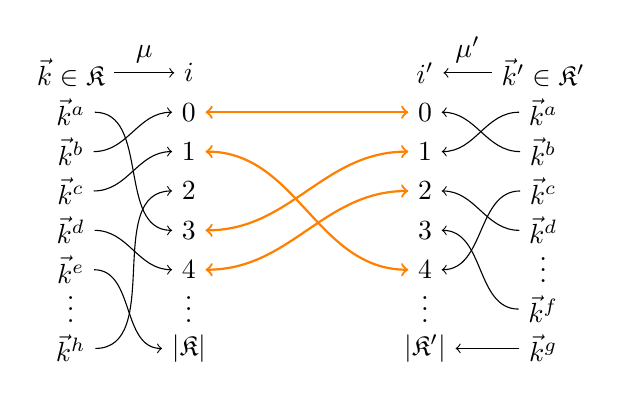
\begin{tikzpicture}[%
    node distance=0.5cm, auto,
    func/.style={scale=0.8,color=gray},
    zero/.style={scale=0.8,color=gray}]

    \node (ko) {$\vec{k} \in \mathfrak{K}$};
    \node (io) [right of=ko, node distance=1.5cm] {$i$};
    \draw[->] (ko) to node {$\mu$} (io);

    \node (ko0) [below of=ko] {$\vec{k}^a$};
    \node (ko1) [below of=ko0] {$\vec{k}^b$};
    \node (ko2) [below of=ko1] {$\vec{k}^c$};
    \node (ko3) [below of=ko2] {$\vec{k}^d$};
    \node (ko4) [below of=ko3] {$\vec{k}^e$};
    \node (ko5) [below of=ko4, node distance=4mm] {$\vdots$};
    \node (ko6) [below of=ko5, node distance=6mm] {$\vec{k}^h$};

    \node (io0) [below of=io] {$0$};
    \node (io1) [below of=io0] {$1$};
    \node (io2) [below of=io1] {$2$};
    \node (io3) [below of=io2] {$3$};
    \node (io4) [below of=io3] {$4$};
    \node (io5) [below of=io4, node distance=4mm] {$\vdots$};
    \node (io6) [below of=io5, node distance=6mm] {$|\mathfrak{K}|$};

    \draw[->] (ko0) to[out=0,in=180] node {} (io3);
    \draw[->] (ko1) to[out=0,in=180] node {} (io0);
    \draw[->] (ko2) to[out=0,in=180] node {} (io1);
    \draw[->] (ko3) to[out=0,in=180] node {} (io4);
    \draw[->] (ko4) to[out=0,in=180] node {} (io6);
    \draw[->] (ko6) to[out=0,in=180] node {} (io2);

    \node (ip) [right of=io, node distance=3cm] {$i^\prime$};
    \node (kp) [right of=ip, node distance=1.5cm] {$\vec{k}^\prime \in \mathfrak{K}^\prime$};
    \draw[<-] (ip) to node {$\mu^\prime$} (kp);

    \node (kp0) [below of=kp] {$\vec{k}^a$};
    \node (kp1) [below of=kp0] {$\vec{k}^b$};
    \node (kp2) [below of=kp1] {$\vec{k}^c$};
    \node (kp3) [below of=kp2] {$\vec{k}^d$};
    \node (kp4) [below of=kp3, node distance=4mm] {$\vdots$};
    \node (kp5) [below of=kp4, node distance=6mm] {$\vec{k}^f$};
    \node (kp6) [below of=kp5] {$\vec{k}^g$};

    \node (ip0) [below of=ip] {$0$};
    \node (ip1) [below of=ip0] {$1$};
    \node (ip2) [below of=ip1] {$2$};
    \node (ip3) [below of=ip2] {$3$};
    \node (ip4) [below of=ip3] {$4$};
    \node (ip5) [below of=ip4, node distance=4mm] {$\vdots$};
    \node (ip6) [below of=ip5, node distance=6mm] {$|\mathfrak{K}^\prime|$};

    \draw[->] (kp0) to[out=180,in=0] node {} (ip1);
    \draw[->] (kp1) to[out=180,in=0] node {} (ip0);
    \draw[->] (kp2) to[out=180,in=0] node {} (ip4);
    \draw[->] (kp3) to[out=180,in=0] node {} (ip2);
    \draw[->] (kp5) to[out=180,in=0] node {} (ip3);
    \draw[->] (kp6) to[out=180,in=0] node {} (ip6);

    \draw[thick, <->, color=orange] (io0) to[out=0,in=180] node {} (ip0);
    \draw[thick, <->, color=orange] (io1) to[out=0,in=180] node {} (ip4);
    \draw[thick, <->, color=orange] (io3) to[out=0,in=180] node {} (ip1);
    \draw[thick, <->, color=orange] (io4) to[out=0,in=180] node {} (ip2);
\end{tikzpicture}

  \caption[Basis shape transformation mapping]
  {The two mappings $\mu$ and $\mu^\prime$ together with the transformation rule $T$ (orange arrows).}
  \label{fig:map}
\end{figure}

When remapping linearly indexed data vectors $\vec{c}_{\mu\left(\vec{k}\right)}$,
we drop the entries for all $\vec{k} \in \mathfrak{K} \setminus \mathfrak{K}^\prime$
and we fill in zero values for all $\vec{k} \in \mathfrak{K}^\prime \setminus \mathfrak{K}$.
The procedure is shown in algorithm \ref{al:basis_shape_remapping} below.

\begin{algorithm}
  \caption{Transformation of basis shapes and data remapping}
  \label{al:basis_shape_remapping}
  \begin{algorithmic}
    \REQUIRE The old basis shape $\mathfrak{K}$
    \REQUIRE The new basis shape $\mathfrak{K}^\prime$
    \REQUIRE An array $\vec{c}$ of length $|\mathfrak{K}|$ containing arbitrary data
    \STATE // Set up the new array of length $|\mathfrak{K}^\prime|$
    \STATE $\vec{c}^\prime \assign \vec{0} \in \mathbb{C}^{|\mathfrak{K}^\prime|}$
    \STATE // Copy over the data we can keep
    \FOR{$\vec{k} \in \mathfrak{K} \cap \mathfrak{K}^\prime$}
      \STATE // Compute linear mapping of $\vec{k}$ in both basis shapes
      \STATE $i \assign \mu\left(\vec{k}\right)$
      \STATE $j \assign \mu^\prime\left(\vec{k}\right)$
      \STATE // Update the array
      \STATE $\vec{c}^\prime\left[j\right] = \vec{c}\left[i\right]$
    \ENDFOR
  \end{algorithmic}
\end{algorithm}

An example of such a mapping is given in figure \ref{fig:trafo_map}.

\begin{figure}
  \centering
  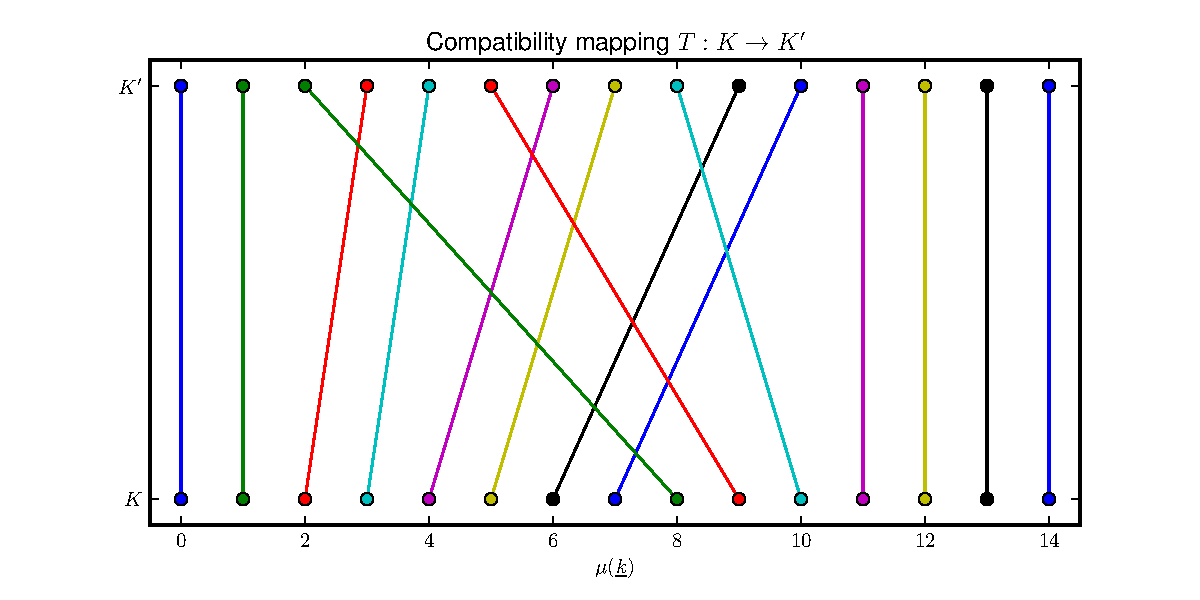
\includegraphics[scale=0.5]{./fig/trafo_map.pdf}
  \caption[Transformation mapping example]
          {An example of a basis shape transformation mapping $T$. The original
          shape was $\mathfrak{K} = \vec{K} = (4,2)$ and $|\mathfrak{K}| = 8$ while
          the new shape is $\mathfrak{K}^{\prime} = \vec{K}^{\prime} = (5,3)$ and
          $|\mathfrak{K}^{\prime}| = 15$.}
  \label{fig:trafo_map}
\end{figure}


\subsection{Basis shape extensions}


For computing the gradients of wavepackets (see section \ref{sec:gradient_computation})
we need to extend the basis shape. Informally spoken, extending a basis shape
means that we add a node in each direction. For each lattice point of a shape
we add all its neighbours. A formal definition is:

\begin{definition}[Basis shape extension]
  Given a basis shape $\mathfrak{K}$ we define its extension $\overline{\mathfrak{K}}$ by:
  \begin{equation*}
    \overline{\mathfrak{K}} \assign \mathfrak{K}
                            \cup \left\{ \vec{k}^\prime : \vec{k}^\prime = \vec{k} + \vec{e}^d \,\forall\, d \in [0,\ldots,D-1]
                                                          \,\forall\, \vec{k} \in \mathfrak{K} \right\} \,.
  \end{equation*}
  This defines the most tight extension. But any even larger basis shape is a
  valid extension too. In any case it holds that $\mathfrak{K} \subset \overline{\mathfrak{K}}$.
\end{definition}

This definition is not handy enough to work with. For some of the less complex basis
shapes $\mathfrak{K}(\theta)$ it is often possible to express the extended shape
$\overline{\mathfrak{K}(\theta^\prime)}$ simply by modifying the parameters
$\theta$ the shape depends on.

If we look at a hypercubic basis shape $\mathfrak{K}(\vec{K})$ then we can express
its extension $\overline{\mathfrak{K}(\vec{K}^\prime)}$ by the new parameters
$\vec{K}^\prime$ which obviously are:

\begin{equation} \label{eq:extend_hypercubic}
  \vec{K}^\prime = [ K_0 + 1, \ldots, K_{D-1} +1 ] \,.
\end{equation}

The attentive reader may notice that in case $D > 1$ this new basis
includes one node too much, namely the lattice point $(K_0, \ldots, K_{D-1})$.
This however poses no problems beside wasting a very small amount of memory.
A basis shape extension has not to be tight with respect to the above definition.

For the hyperbolic cut shape, extension is less trivial. Assume that the sparsity is $K$.
We first look at the extension of a two-dimensional shape. Here the two nodes
$(K-1, 0)$ and $(0, K-1)$ are the outermost ones. Since the whole basis shape is
symmetric under permutation of the axes, we focus only on $(K-1, 0)$ lying on the first
axis. We have to make sure that its neighbours are part of $\overline{\mathfrak{K}}$.
This is guaranteed (by definition \ref{def:hyperbolic_cut_shape}) if we can
construct a new hyperbolic cut shape $\mathfrak{K}^\prime(K^\prime)$ that
contains the node $(K-1,1)$. By using the equation of the above definition we get:

\begin{equation*}
  (1+K-1)(1+1) \leq K^\prime
\end{equation*}

which we can solve for the minimal $K^\prime$ and find that:

\begin{equation} \label{eq:extend_hyperbolic_cut_1D}
  K^\prime = 2 K \,.
\end{equation}

In the general case of $D>1$ dimensions we have a similar equation:

\begin{align*}
  (1+K-1)(1+1)\cdots(1+1) & = (1+K-1)\left(\prod_{d=1}^{D-1}(1+1)\right) \leq K^\prime
\end{align*}

from which we obtain:

\begin{equation} \label{eq:extend_hyperbolic_cut_DD}
  K^\prime = 2^{D-1} K \,.
\end{equation}

This is only valid for $D>1$ and gives for $D=1$ the wrong result $K^\prime = K$.
If we want a single formula valid for all dimensions then we have to start from
the point $\vec{k} = (K, 0, \ldots, 0)$. For this point we get:

\begin{align*}
  (1+K)\left(\prod_{d=1}^{D-1}(1+1)\right) \leq K^\prime
\end{align*}

giving:

\begin{equation} \label{eq:extend_hyperbolic_cut_general}
  K^\prime = 2^{D-1} (K+1) \,.
\end{equation}

However we should note that this leads to overly big extensions for $D>1$
compared to the other formula. For example if we start with a two-dimensional
basis shape with $K=4$ then we get $K^\prime = 8$ and $K^\prime = 10$ respectively.
The basis sizes of the extended shapes are then $20$ and $27$ and the tight extension
given by the direct definition would have size $14$ but is not of hyperbolic
cut type.

Extending a hyperbolic cut basis shape with limits is easy again. First we change
the limits $\vec{L}$ according to \eqref{eq:extend_hypercubic}. Then we increase $K$
by using one of the formulae \eqref{eq:extend_hyperbolic_cut_1D} or
\eqref{eq:extend_hyperbolic_cut_DD} depending on the dimensionality.
That is all we need to do for this type of basis shape.

We can use the limited hyperbolic cut basis shape to produce more tight extensions
of the standard hyperbolic cut basis shapes. For an example, refer to figure
\ref{fig:hyperbolic_extensions_compared}.

\begin{figure}
  \centering
  \subfloat[][]{
    \label{fig:hyperbolic_extension}
    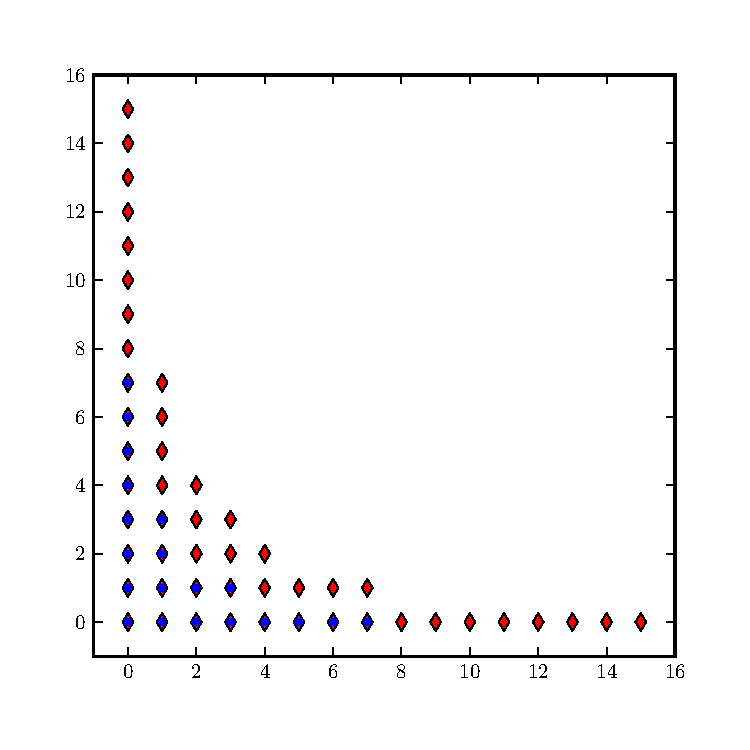
\includegraphics[width=0.5\linewidth]{./fig/hyperbolic_extension.pdf}
  }
  \subfloat[][]{
    \label{fig:hyperbolic_limited}
    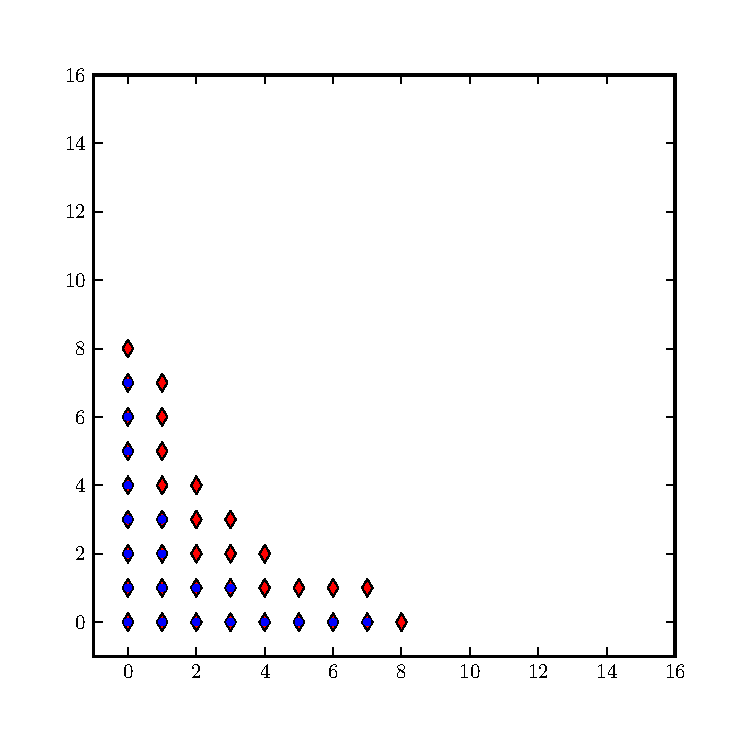
\includegraphics[width=0.5\linewidth]{./fig/hyperbolic_extension_limited.pdf}
  } \\
  \caption[Extensions of a hyperbolic cut basis shape]{
    Comparison of two methods to extend a hyperbolic cut basis shape with $K=8$.
    The original nodes (blue circles) and the nodes of the extension (red diamonds)
    are shown for both methods. The difference in basis size is $14$ nodes.
    \subref{fig:hyperbolic_extension} Extension is again an unlimited hyperbolic
                                      cut shape with $K = 16$.
    \subref{fig:hyperbolic_limited} Extension is a limited hyperbolic cut shape
                                    with $K = 16$ and $\vec{L} = (9,9)$. This extension
                                    introduces only $3$ nodes more than required.
    \label{fig:hyperbolic_extensions_compared}
  }
\end{figure}


\section{Evaluation of wavepackets}


For the numerical simulation we will need to evaluate a wavepacket at sets of
grid nodes $\vec{\gamma} \in \mathbb{R}^D$. The formula for the ground state
\eqref{eq:phi0_Dd} and the recursion \eqref{eq:basis_recursion_DD} for higher
order basis functions is in principle all we need to do this. Even if this
seems to be very simple at first glance there are a few tricky details involved.
In this section we start from the mathematical formulae and work towards an
algorithmic description for computing $\Phi(\vec{\gamma})$.

First we can evaluate the ground state $\phi_{\vec{0}}$ directly by algorithm \ref{al:eval_phi0_DD}.
If this is programmed by using vectorisation for the linear algebra functions we
can even perform the evaluation on a set $\Gamma = \{\gamma_i\}_i$ of nodes simultaneously.
The return value is then not a single scalar value but an array of scalars.
Usually we imagine this to be a row vector of $|\Gamma|$ elements.

\begin{algorithm}
\caption{Evaluate the ground state $\phi_0$ directly}
\label{al:eval_phi0_DD}
\begin{algorithmic}
  \REQUIRE The number $D$ of space dimensions
  \REQUIRE The Hagedorn parameter set $\Pi = \{q,p,Q,P\}$
  \REQUIRE The semi-classical scaling parameter $\varepsilon$
  \REQUIRE The grid node $\vec{\gamma} \in \mathbb{R}^D$

  \STATE // Whether to include the problematic prefactor or not
  \IF{prefactor is True}
    \STATE $\alpha \assign (\pi\varepsilon^2)^{-\frac{D}{4}} (\det\mat{Q})^{-\frac{1}{2}}$
  \ELSE
    \STATE $\alpha \assign (\pi\varepsilon^2)^{-\frac{D}{4}}$
  \ENDIF

  \STATE // The exponent
  \STATE $\vec{u} \assign \vec{\gamma}-\vec{q}$
  \STATE $\beta_1 \assign \dotp{\vec{u}}{\mat{P}\mat{Q}\inv\vec{u}}$
  \STATE $\beta_2 \assign \dotp{\vec{p}}{\vec{u}}$

  \STATE // The full ground state
  \STATE $\phi_{\vec{0}} \assign \alpha \exp\left(\frac{i}{\varepsilon^2}\left(\frac{1}{2}\beta_1 + \beta_2\right)\right)$

  \RETURN $\phi_{\vec{0}}$
\end{algorithmic}
\end{algorithm}

For the higher order basis functions $\phi_{\vec{k}}$ we employ the recursion
formula. With the help of this relation we can compute any $\phi_{\vec{k}}$
given some of the predecessors. For $D=1$ this is easy since we just compute
$\phi_{k+1}$ from $\phi_k$ and $\phi_{k-1}$. In the multi-dimensional case
it is less obvious what happens. To compute the set of all successors $\{\phi_{\vec{k}+\vec{e}^d}\}_{d=0}^{D-1}$
we need the function $\phi_{\vec{k}}$ as well as all antecessors $\{\phi_{\vec{k}-\vec{e}^d}\}_{d=0}^{D-1}$.
We call this rule that specifies how we get new functions from old ones a \emph{stencil}
and denote it by $\mathcal{S}^D$. The figure \ref{fig:recursion_stencils_full}
shows the stencils we get in one, two and three dimensions.

\begin{figure}[h!]
  \centering
  \subfloat[][$\mathcal{S}^1$]{
    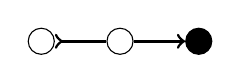
\begin{tikzpicture}[%
  wnode/.style={circle,fill=white,draw},
  bnode/.style={circle,fill=black,draw},
  thickline/.style={line width=1pt}]
  \node[wnode] (O) {};
  \node[wnode] (O1) [left of=O]  {};
  \node[bnode] (N1) [right of=O] {};
  \path[thickline, >-] (O1) edge (O);
  \draw[thickline,->] (O) to node {} (N1);
\end{tikzpicture}

  }
  \subfloat[][$\mathcal{S}^2$]{
    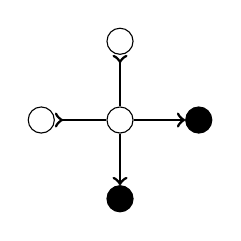
\begin{tikzpicture}[%
  wnode/.style={circle,fill=white,draw},
  bnode/.style={circle,fill=black,draw},
  thickline/.style={line width=1pt}]
  \node[wnode] (O) {};
  \node[wnode] (O1) [left of=O]  {};
  \node[wnode] (O2) [above of=O]  {};
  \node[bnode] (N1) [right of=O] {};
  \node[bnode] (N2) [below of=O] {};
  \path[thickline, >-] (O1) edge (O);
  \path[thickline, >-] (O2) edge (O);
  \draw[thickline,->] (O) to node {} (N1);
  \draw[thickline,->] (O) to node {} (N2);
\end{tikzpicture}

  }
  \subfloat[][$\mathcal{S}^3$]{
    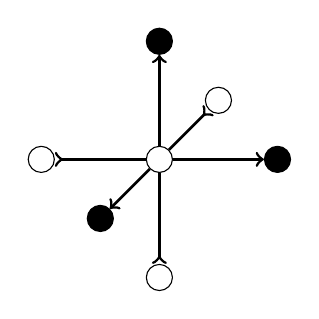
\begin{tikzpicture}[%
  node distance=1.5cm, auto,
  wnode/.style={circle,fill=white,draw},
  bnode/.style={circle,fill=black,draw},
  thickline/.style={line width=1pt}]
  \node[wnode] (O) {};
  \node[wnode] [left of=O] (O1) {};
  \node[wnode] [right of=O, above of=O, node distance=0.75cm] (O2) {};
  \node[wnode] [below of=O] (O3) {};
  \node[bnode] (N1) [right of=O] {};
  \node[bnode] (N2) [left of=O, below of=O, node distance=0.75cm] {};
  \node[bnode] (N3) [above of=O] {};
  \path[thickline, >-] (O1) edge (O);
  \path[thickline, >-] (O2) edge (O);
  \path[thickline, >-] (O3) edge (O);
  \draw[thickline,->] (O) to node {} (N1);
  \draw[thickline,->] (O) to node {} (N2);
  \draw[thickline,->] (O) to node {} (N3);
\end{tikzpicture}

  } \\
    \caption[Full recursion stencils in one, two and three dimensions]{The basis
    function recursion stencils in one, two and three dimensions. The black nodes
    can be computed given the white ones. This works in one single step, i.e.
    we need all white ones and get all black ones.}
    \label{fig:recursion_stencils_full}
\end{figure}

For all these recurrences we need starting points. The only point we know is $\phi_{\vec{0}}$.
But as we found earlier we can insert a $0$ for all $\vec{k}$ where $\exists k_d$ with $k_d < 0$.
Hence we have indeed enough known values to get the process started. An example
of how this works in two dimensions is shown in figure \ref{fig:naive_stencil_application}
and algorithm \ref{al:eval_phik_DD_naive}.

\begin{figure}
  \centering
  \begin{tikzpicture}[%
    func/.style={scale=0.8,color=gray},
    zero/.style={scale=0.8,color=black}]

    \node[zero] (v0m1) at (1,0) {$0$};
    \node[zero] (v1m1) at (2,0) {$0$};
    \node[zero] (v2m1) at (3,0) {$0$};
    \node[zero] (v3m1) at (4,0) {$0$};

    \node[zero] (vm10) at (0,1) {$0$};
    \node[zero] (vm11) at (0,2) {$0$};
    \node[zero] (vm12) at (0,3) {$0$};
    \node[zero] (vm13) at (0,4) {$0$};

    \node[func,color=black] (v00) at (1,1) {$\phi_{0,0}$};

    \node[func,color=blue] (v01) at (1,2) {$\phi_{0,1}$};
    \node[func,color=green] (v02) at (1,3) {$\phi_{0,2}$};
    \node[func] (v03) at (1,4) {$\phi_{0,3}$};

    \node[func,color=blue] (v10) at (2,1) {$\phi_{1,0}$};
    \node[func,color=green] (v11) at (2,2) {$\phi_{1,1}$};
    \node[func] (v12) at (2,3) {$\phi_{1,2}$};
    \node[func] (v13) at (2,4) {$\phi_{1,3}$};

    \node[func,color=green] (v20) at (3,1) {$\phi_{2,0}$};
    \node[func] (v21) at (3,2) {$\phi_{2,1}$};
    \node[func] (v22) at (3,3) {$\phi_{2,2}$};
    \node[func] (v23) at (3,4) {$\phi_{2,3}$};

    \node[func] (v30) at (4,1) {$\phi_{3,0}$};
    \node[func] (v31) at (4,2) {$\phi_{3,1}$};
    \node[func] (v32) at (4,3) {$\phi_{3,2}$};
    \node[func] (v33) at (4,4) {$\phi_{3,3}$};

    \begin{scope}
    \draw[draw=green!80,line width=0.8pt] ($(v10)+(0.0,0.3)$)
        to[out=190,in=350] ($(v00)+(0.0,0.3)$)
        to[out=170,in=90] ($(v00)+(-0.3,0.0)$)
        to[out=270,in=190] ($(v00)+(0.0,-0.3)$)
        to[out=10,in=80] ($(v1m1)+(-0.2,0.0)$)
        to[out=260,in=180] ($(v1m1)+(0.0,-0.2)$)
        to[out=0,in=280] ($(v1m1)+(0.2,0.0)$)
        to[out=100,in=260] ($(v10)+(0.3,0.0)$)
        to[out=80,in=10] ($(v10)+(0.0,0.3)$);
    \draw[draw=green!80,->,line width=0.8pt] ($(v10)+(0.0,0.3)$) -- (v11);
    \draw[draw=green!80,->,line width=0.8pt] ($(v10)+(0.3,0.0)$) -- (v20);
    \end{scope}

    \begin{scope}
    \draw[draw=green!80,line width=0.8pt] ($(v01)+(0.0,0.3)$)
        to[out=190,in=350] ($(vm11)+(0.0,0.2)$)
        to[out=170,in=90] ($(vm11)+(-0.2,0.0)$)
        to[out=270,in=190] ($(vm11)+(0.0,-0.2)$)
        to[out=10,in=80] ($(v00)+(-0.3,0.0)$)
        to[out=260,in=180] ($(v00)+(0.0,-0.3)$)
        to[out=0,in=280] ($(v00)+(0.3,0.0)$)
        to[out=100,in=260] ($(v01)+(0.3,0.0)$)
        to[out=80,in=10] ($(v01)+(0.0,0.3)$);
    \draw[draw=green!80,->,line width=0.8pt] ($(v01)+(0.0,0.3)$) -- (v02);
    \draw[draw=green!80,->,line width=0.8pt] ($(v01)+(0.3,0.0)$) -- (v11);
    \end{scope}

    \begin{scope}
    \draw[draw=blue!100,line width=0.8pt] ($(v00)+(0.0,0.3)$)
        to[out=190,in=350] ($(vm10)+(0.0,0.2)$)
        to[out=170,in=90] ($(vm10)+(-0.2,0.0)$)
        to[out=270,in=190] ($(vm10)+(0.0,-0.2)$)
        to[out=10,in=80] ($(v0m1)+(-0.2,0.0)$)
        to[out=260,in=180] ($(v0m1)+(0.0,-0.2)$)
        to[out=0,in=280] ($(v0m1)+(0.2,0.0)$)
        to[out=100,in=260] ($(v00)+(0.3,0.0)$)
        to[out=80,in=10] ($(v00)+(0.0,0.3)$);
    \draw[draw=blue,->,line width=0.8pt] ($(v00)+(0.0,0.3)$) -- (v01);
    \draw[draw=blue,->,line width=0.8pt] ($(v00)+(0.3,0.0)$) -- (v10);
    \end{scope}
\end{tikzpicture}

  \caption[Naive stencil application in two dimensions]{Naive stencil application
           in two dimensions. All values we initially know are printed in black.
           In a first step we centre the stencil $\mathcal{S}^2$ at the node
           $\vec{k} = (0,0)$ (blue) and compute $\phi_{0,1}$ and $\phi_{1,0}$.
           Next we can apply the stencil there (green) and find $\phi_{0,2}$,
           $\phi_{1,1}$ and $\phi_{2,0}$.}
  \label{fig:naive_stencil_application}
\end{figure}

\begin{algorithm}
  \caption{Evaluate higher order states $\phi_k$ recursively (naive version)}
  \label{al:eval_phik_DD_naive}
  \begin{algorithmic}
    \REQUIRE The number $D$ of space dimensions
    \REQUIRE The Hagedorn parameter set $\Pi = \{q,p,Q,P\}$
    \REQUIRE The semi-classical scaling parameter $\varepsilon$
    \REQUIRE The basis shape $\mathfrak{K}$ and its linearisation mapping $\mu$
    \REQUIRE The grid node $\vec{\gamma} \in \mathbb{R}^D$

    \STATE // Storage space for the result
    \STATE $\vec{\psi} \assign \vec{0} \in \mathbb{C}^{|\mathfrak{K}|}$

    \STATE // Evaluate the ground state by algorithm \ref{al:eval_phi0_DD}
    \STATE $\vec{\psi}[\mu(\vec{0})] = \text{\bf{evaluate\_ground\_state}}(D, \Pi, \varepsilon, \vec{\gamma})$

    \STATE // Loop over the multi-indices
    \FOR{$\vec{k} \in \mathfrak{K}$}
      \STATE // Backward neighbours
      \STATE $\vec{\xi} \assign \vec{0} \in \mathbb{C}^{D}$
      \FOR{$d = 0$ \TO $d = D-1$}
        \STATE $\vec{k}^\prime \assign \vec{k} - \vec{e}^{d}$
        \IF{$\vec{k}^\prime \in \mathfrak{K}$}
          \STATE $\vec{\xi}[d] = \sqrt{\vec{k}[d]} \, \vec{\psi}[\mu(\vec{k}^\prime)]$
        \ENDIF
      \ENDFOR

      \STATE // Compute 3-term recursion
      \STATE $\vec{\alpha} \assign (\vec{\gamma} - \vec{q}) \, \vec{\psi}[\mu(\vec{k})]$
      \STATE $\vec{\beta_1} \assign \sqrt{\frac{2}{\varepsilon^2}} \, \mat{Q}\inv \cdot \vec{\alpha}$
      \STATE $\vec{\beta_2} \assign \mat{Q}\inv \conj{\mat{Q}} \cdot \vec{\xi}$
      \STATE $\vec{\beta} \assign \vec{\beta_1} - \vec{\beta_2}$

      \STATE // Store the results at the correct positions (forward neighbours)
      \FOR{$d = 0$ \TO $d = D-1$}
        \STATE $\vec{k}^\prime \assign \vec{k} + \vec{e}^d$
        \IF{$\vec{k}^\prime \in \mathfrak{K}$}
          \STATE $\vec{\psi}[\mu(\vec{k}^\prime)] = \frac{\vec{\beta}[d]}{\sqrt{\vec{k}[d] + 1}}$
        \ENDIF
      \ENDFOR
  \ENDFOR

  \STATE // Whether to include the problematic prefactor or not
  \STATE // Make sure not to divide twice for $\phi_{\vec{0}}$!
  \IF{prefactor is True}
    \STATE $\vec{\psi} = \frac{1}{\sqrt{\det\mat{Q}}} \, \vec{\psi}$
  \ENDIF

  \RETURN $\vec{\psi}$
\end{algorithmic}
\end{algorithm}

The most severe issue with this naive stencil application is that we compute almost
all functions twice, here this becomes obvious the first time for $\phi_{1,1}$.
Even worse, in $D$ dimensions we would compute almost all functions $D$ times!

Therefore we seek a better way to organise the computations. To achieve this goal we
modify the stencil in a way that seems to be counter intuitive at first. Define the
modified \emph{cheap stencil} as follows.

\begin{definition}[Cheap recursion stencil]
  The cheap recursion stencil does not compute all $D$ outputs $\phi_{\vec{k}+\vec{e}^d}$
  for all $d \in [0, \ldots, D-1]$ but only one output for a single and fixed direction $d$.
  We denote the cheap stencil for direction $d$ and in $D$ dimensions by $\mathcal{S}_d^D$.
  In $D$ dimensions we have $D$ different stencils:
  \begin{equation*}
    \mathcal{S}^D_d \quad d \in [0, \ldots, D-1] \, .
  \end{equation*}
\end{definition}

Figures \ref{fig:recursion_stencils_cheap_2D} and \ref{fig:recursion_stencils_cheap_3D}
give an impression how the stencils look like and how they work in two and three
dimensions. In one dimension we obviously find $\mathcal{S}^1_0 \equiv \mathcal{S}^1$.
In all dimensions it holds that we recover the full stencil $\mathcal{S}^D$ as the sum:

\begin{equation*}
  \mathcal{S}^D = \bigoplus_{d=0}^{D-1} \mathcal{S}^D_d
\end{equation*}

where all stencils are applied centred at the very same node $\phi_{\vec{k}}$.

\begin{figure}[h!]
  \centering
  \subfloat[][$\mathcal{S}^2_0$]{
    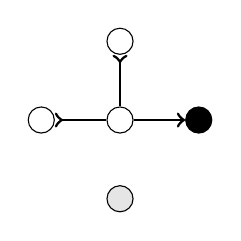
\begin{tikzpicture}[%
  wnode/.style={circle,fill=white,draw},
  bnode/.style={circle,fill=black,draw},
  gnode/.style={circle,fill=black!10,draw},
  thickline/.style={line width=1pt}]
  \node[wnode] (O) {};
  \node[wnode] (O1) [left of=O]  {};
  \node[wnode] (O2) [above of=O]  {};
  \node[bnode] (N1) [right of=O] {};
  \node[gnode] (N2) [below of=O] {};
  \path[thickline, >-] (O1) edge (O);
  \path[thickline, >-] (O2) edge (O);
  \draw[thickline,->] (O) to node {} (N1);
\end{tikzpicture}

  }
  \subfloat[][$\mathcal{S}^2_1$]{
    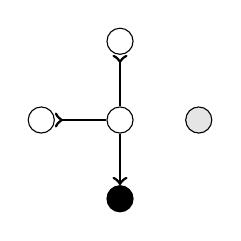
\begin{tikzpicture}[%
  wnode/.style={circle,fill=white,draw},
  bnode/.style={circle,fill=black,draw},
  gnode/.style={circle,fill=black!10,draw},
  thickline/.style={line width=1pt}]
  \node[wnode] (O) {};
  \node[wnode] (O1) [left of=O]  {};
  \node[wnode] (O2) [above of=O]  {};
  \node[gnode] (N1) [right of=O] {};
  \node[bnode] (N2) [below of=O] {};
  \path[thickline, >-] (O1) edge (O);
  \path[thickline, >-] (O2) edge (O);
  \draw[thickline,->] (O) to node {} (N2);
\end{tikzpicture}

  } \\
    \caption[Cheap recursion stencils in two dimensions]{The modified basis
    function recursion stencils $\mathcal{S}^2_d$ in two dimensions.
    The black node can be computed given the white nodes. The grey node would be
    computed by the full stencil $\mathcal{S}^2$ but is intentionally left out by
    the modified ones.}
    \label{fig:recursion_stencils_cheap_2D}
\end{figure}

\begin{figure}[h!]
  \centering
  \subfloat[][$\mathcal{S}^3_0$]{
    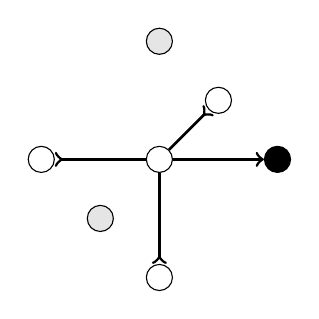
\begin{tikzpicture}[%
  node distance=1.5cm, auto,
  wnode/.style={circle,fill=white,draw},
  bnode/.style={circle,fill=black,draw},
  gnode/.style={circle,fill=black!10,draw},
  thickline/.style={line width=1pt}]
  \node[wnode] (O) {};
  \node[wnode] [left of=O] (O1) {};
  \node[wnode] [right of=O, above of=O, node distance=0.75cm] (O2) {};
  \node[wnode] [below of=O] (O3) {};
  \node[bnode] (N1) [right of=O] {};
  \node[gnode] (N2) [left of=O, below of=O, node distance=0.75cm] {};
  \node[gnode] (N3) [above of=O] {};
  \path[thickline, >-] (O1) edge (O);
  \path[thickline, >-] (O2) edge (O);
  \path[thickline, >-] (O3) edge (O);
  \draw[thickline,->] (O) to node {} (N1);
\end{tikzpicture}

  }
  \subfloat[][$\mathcal{S}^3_1$]{
    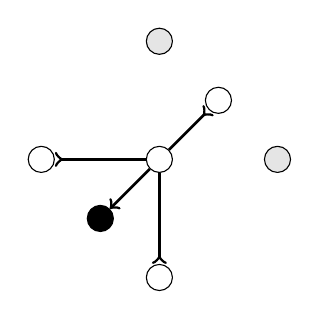
\begin{tikzpicture}[%
  node distance=1.5cm, auto,
  wnode/.style={circle,fill=white,draw},
  bnode/.style={circle,fill=black,draw},
  gnode/.style={circle,fill=black!10,draw},
  thickline/.style={line width=1pt}]
  \node[wnode] (O) {};
  \node[wnode] [left of=O] (O1) {};
  \node[wnode] [right of=O, above of=O, node distance=0.75cm] (O2) {};
  \node[wnode] [below of=O] (O3) {};
  \node[gnode] (N1) [right of=O] {};
  \node[bnode] (N2) [left of=O, below of=O, node distance=0.75cm] {};
  \node[gnode] (N3) [above of=O] {};
  \path[thickline, >-] (O1) edge (O);
  \path[thickline, >-] (O2) edge (O);
  \path[thickline, >-] (O3) edge (O);
  \draw[thickline,->] (O) to node {} (N2);
\end{tikzpicture}

  }
  \subfloat[][$\mathcal{S}^3_2$]{
    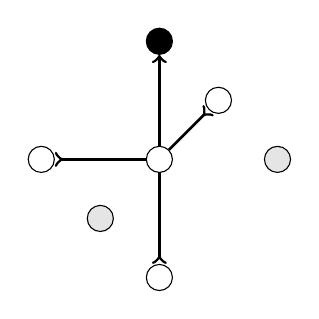
\begin{tikzpicture}[%
  node distance=1.5cm, auto,
  wnode/.style={circle,fill=white,draw},
  bnode/.style={circle,fill=black,draw},
  gnode/.style={circle,fill=black!10,draw},
  thickline/.style={line width=1pt}]
  \node[wnode] (O) {};
  \node[wnode] [left of=O] (O1) {};
  \node[wnode] [right of=O, above of=O, node distance=0.75cm] (O2) {};
  \node[wnode] [below of=O] (O3) {};
  \node[gnode] (N1) [right of=O] {};
  \node[gnode] (N2) [left of=O, below of=O, node distance=0.75cm] {};
  \node[bnode] (N3) [above of=O] {};
  \path[thickline, >-] (O1) edge (O);
  \path[thickline, >-] (O2) edge (O);
  \path[thickline, >-] (O3) edge (O);
  \draw[thickline,->] (O) to node {} (N3);
\end{tikzpicture}

  } \\
    \caption[Cheap recursion stencils in three dimensions]{The modified basis
    function recursion stencils $\mathcal{S}^3_d$ in three dimensions.
    The black node can be computed given the white nodes. The grey nodes would be
    computed by the full stencil $\mathcal{S}^3$ but is intentionally left out by
    the modified ones.}
    \label{fig:recursion_stencils_cheap_3D}
\end{figure}

Formally we have just used the $d$-th row of equation \eqref{eq:basis_recursion_DD} only
to compute the application of $\mathcal{S}^D_d$ to $\phi_{\vec{k}}$. By using colon or
slicing notation we can write the formula for the modified stencils $\mathcal{S}^D_d$
as follows:

\begin{equation}
  \sqrt{k_d +1} \phi_{k + e_d}
  = \sqrt{\frac{2}{\varepsilon^2}}
  \left(Q^{-1}\right)_{d,:}
  \left( x-q \right)
  \phi_{k}
  -
  \left(Q^{-1} \overline{Q} \right)_{d,:}
  \begin{pmatrix}
    \sqrt{k_0} \phi_{k - e_0} \\
    \vdots \\
    \sqrt{k_{D-1}} \phi_{k - e_{D-1}}
  \end{pmatrix} \,.
\end{equation}

What can we do with these modified stencils? And why should they be more efficient?
The most important gain is that we do never compute any function twice. But for this
we have to use the new stencils in a clever way. We start with an empty grid like the
one in figure \ref{fig:naive_stencil_application}. It contains only the ground state
evaluated $\phi_{\vec{0}}$. Now we apply the stencil $\mathcal{S}^D_0$ along the first
direction $d=0$ until we overflow. This works fine as we use the ground state as
anchor point for this \emph{recursion chain} and produce new anchor points successively.
This process is shown in figure \ref{fig:efficient_stencil_application_d0}.

\begin{figure}
  \centering
  \begin{tikzpicture}[%
    func/.style={scale=0.8,color=gray},
    zero/.style={scale=0.8,color=black}]

    \node[zero] (v0m1) at (1,0) {$0$};
    \node[zero] (v1m1) at (2,0) {$0$};
    \node[zero] (v2m1) at (3,0) {$0$};
    \node[zero] (v3m1) at (4,0) {$0$};

    \node[zero] (vm10) at (0,1) {$0$};
    \node[zero] (vm11) at (0,2) {$0$};
    \node[zero] (vm12) at (0,3) {$0$};
    \node[zero] (vm13) at (0,4) {$0$};

    \node[func,color=black] (v00) at (1,1) {$\phi_{0,0}$};

    \node[func] (v01) at (1,2) {$\phi_{0,1}$};
    \node[func] (v02) at (1,3) {$\phi_{0,2}$};
    \node[func] (v03) at (1,4) {$\phi_{0,3}$};

    \node[func,color=blue] (v10) at (2,1) {$\phi_{1,0}$};
    \node[func] (v11) at (2,2) {$\phi_{1,1}$};
    \node[func] (v12) at (2,3) {$\phi_{1,2}$};
    \node[func] (v13) at (2,4) {$\phi_{1,3}$};

    \node[func,color=blue] (v20) at (3,1) {$\phi_{2,0}$};
    \node[func] (v21) at (3,2) {$\phi_{2,1}$};
    \node[func] (v22) at (3,3) {$\phi_{2,2}$};
    \node[func] (v23) at (3,4) {$\phi_{2,3}$};

    \node[func,color=blue] (v30) at (4,1) {$\phi_{3,0}$};
    \node[func] (v31) at (4,2) {$\phi_{3,1}$};
    \node[func] (v32) at (4,3) {$\phi_{3,2}$};
    \node[func] (v33) at (4,4) {$\phi_{3,3}$};

    \begin{scope}
    \draw[draw=blue!60,line width=0.8pt] ($(v20)+(0.0,0.3)$)
        to[out=190,in=350] ($(v10)+(0.0,0.3)$)
        to[out=170,in=90] ($(v10)+(-0.3,0.0)$)
        to[out=270,in=190] ($(v10)+(0.0,-0.3)$)
        to[out=10,in=80] ($(v2m1)+(-0.2,0.0)$)
        to[out=260,in=180] ($(v2m1)+(0.0,-0.2)$)
        to[out=0,in=280] ($(v2m1)+(0.2,0.0)$)
        to[out=100,in=260] ($(v20)+(0.3,0.0)$)
        to[out=80,in=10] ($(v20)+(0.0,0.3)$);
    \draw[draw=blue!60,->,line width=0.8pt] ($(v20)+(0.3,0.0)$) -- (v30);
    \end{scope}

    \begin{scope}
    \draw[draw=blue!80,line width=0.8pt] ($(v10)+(0.0,0.3)$)
        to[out=190,in=350] ($(v00)+(0.0,0.3)$)
        to[out=170,in=90] ($(v00)+(-0.3,0.0)$)
        to[out=270,in=190] ($(v00)+(0.0,-0.3)$)
        to[out=10,in=80] ($(v1m1)+(-0.2,0.0)$)
        to[out=260,in=180] ($(v1m1)+(0.0,-0.2)$)
        to[out=0,in=280] ($(v1m1)+(0.2,0.0)$)
        to[out=100,in=260] ($(v10)+(0.3,0.0)$)
        to[out=80,in=10] ($(v10)+(0.0,0.3)$);
    \draw[draw=blue!80,->,line width=0.8pt] ($(v10)+(0.3,0.0)$) -- (v20);
    \end{scope}

    \begin{scope}
    \draw[draw=blue!100,line width=0.8pt] ($(v00)+(0.0,0.3)$)
        to[out=190,in=350] ($(vm10)+(0.0,0.2)$)
        to[out=170,in=90] ($(vm10)+(-0.2,0.0)$)
        to[out=270,in=190] ($(vm10)+(0.0,-0.2)$)
        to[out=10,in=80] ($(v0m1)+(-0.2,0.0)$)
        to[out=260,in=180] ($(v0m1)+(0.0,-0.2)$)
        to[out=0,in=280] ($(v0m1)+(0.2,0.0)$)
        to[out=100,in=260] ($(v00)+(0.3,0.0)$)
        to[out=80,in=10] ($(v00)+(0.0,0.3)$);
    \draw[draw=blue,->,line width=0.8pt] ($(v00)+(0.3,0.0)$) -- (v10);
    \end{scope}
\end{tikzpicture}

  \caption[Efficient stencil application in two dimensions]{
           First step in the efficient application of the recursion stencils
           in two dimensions. All values we initially know are printed in black.
           In a first step we centre the cheap stencil $\mathcal{S}^2_0$ at the
           node $\vec{k} = (0,0)$ and compute $\phi_{1,0}$ only. Next we can use
           the same stencil centred at $\phi_{1,0}$ and find $\phi_{2,0}$. We
           continue like this until an overflow occurs. (In this little example
           we are done after the next step.)}
  \label{fig:efficient_stencil_application_d0}
\end{figure}

After this first step we can not apply the stencil $\mathcal{S}^2_0$ anymore.
There is no anchor point left that would give us new nodes in the lattice.
But we have build a whole chain $\phi_{k, 0}$ of starting points. Hence we take
the stencil $\mathcal{S}^2_1$ at hand and go along the second direction $d=1$
starting a chain for each $\phi_{k,0}$. Again we follow each chain until an
overflow occurs. Note that we must do this in increasing order of the index $k$
because we need the values to the left of where we centre $\mathcal{S}^2_1$.
Figure \ref{fig:efficient_stencil_application_d1} shows the process for the
first two chains starting at $\phi_{0,0}$ and $\phi_{1,0}$.

\begin{figure}[h!]
  \centering
  \subfloat[][]{
    \begin{tikzpicture}[%
    func/.style={scale=0.8,color=gray},
    zero/.style={scale=0.8,color=black}]

    \node[zero] (v0m1) at (1,0) {$0$};
    \node[zero] (v1m1) at (2,0) {$0$};
    \node[zero] (v2m1) at (3,0) {$0$};
    \node[zero] (v3m1) at (4,0) {$0$};

    \node[zero] (vm10) at (0,1) {$0$};
    \node[zero] (vm11) at (0,2) {$0$};
    \node[zero] (vm12) at (0,3) {$0$};
    \node[zero] (vm13) at (0,4) {$0$};

    \node[func,color=black] (v00) at (1,1) {$\phi_{0,0}$};

    \node[func,color=green] (v01) at (1,2) {$\phi_{0,1}$};
    \node[func,color=green] (v02) at (1,3) {$\phi_{0,2}$};
    \node[func,color=green] (v03) at (1,4) {$\phi_{0,3}$};

    \node[func,color=black] (v10) at (2,1) {$\phi_{1,0}$};
    \node[func] (v11) at (2,2) {$\phi_{1,1}$};
    \node[func] (v12) at (2,3) {$\phi_{1,2}$};
    \node[func] (v13) at (2,4) {$\phi_{1,3}$};

    \node[func,color=black] (v20) at (3,1) {$\phi_{2,0}$};
    \node[func] (v21) at (3,2) {$\phi_{2,1}$};
    \node[func] (v22) at (3,3) {$\phi_{2,2}$};
    \node[func] (v23) at (3,4) {$\phi_{2,3}$};

    \node[func,color=black] (v30) at (4,1) {$\phi_{3,0}$};
    \node[func] (v31) at (4,2) {$\phi_{3,1}$};
    \node[func] (v32) at (4,3) {$\phi_{3,2}$};
    \node[func] (v33) at (4,4) {$\phi_{3,3}$};

    \begin{scope}
    \draw[draw=green!60,line width=0.8pt] ($(v02)+(0.0,0.3)$)
        to[out=190,in=350] ($(vm12)+(0.0,0.2)$)
        to[out=170,in=90] ($(vm12)+(-0.2,0.0)$)
        to[out=270,in=190] ($(vm12)+(0.0,-0.2)$)
        to[out=10,in=80] ($(v01)+(-0.3,0.0)$)
        to[out=260,in=180] ($(v01)+(0.0,-0.3)$)
        to[out=0,in=280] ($(v01)+(0.3,0.0)$)
        to[out=100,in=260] ($(v02)+(0.3,0.0)$)
        to[out=80,in=10] ($(v02)+(0.0,0.3)$);
    \draw[draw=green!60,->,line width=0.8pt] ($(v02)+(0.0,0.3)$) -- (v03);
    \end{scope}

    \begin{scope}
    \draw[draw=green!80,line width=0.8pt] ($(v01)+(0.0,0.3)$)
        to[out=190,in=350] ($(vm11)+(0.0,0.2)$)
        to[out=170,in=90] ($(vm11)+(-0.2,0.0)$)
        to[out=270,in=190] ($(vm11)+(0.0,-0.2)$)
        to[out=10,in=80] ($(v00)+(-0.3,0.0)$)
        to[out=260,in=180] ($(v00)+(0.0,-0.3)$)
        to[out=0,in=280] ($(v00)+(0.3,0.0)$)
        to[out=100,in=260] ($(v01)+(0.3,0.0)$)
        to[out=80,in=10] ($(v01)+(0.0,0.3)$);
    \draw[draw=green!80,->,line width=0.8pt] ($(v01)+(0.0,0.3)$) -- (v02);
    \end{scope}

    \begin{scope}
    \draw[draw=green!100,line width=0.8pt] ($(v00)+(0.0,0.3)$)
        to[out=190,in=350] ($(vm10)+(0.0,0.2)$)
        to[out=170,in=90] ($(vm10)+(-0.2,0.0)$)
        to[out=270,in=190] ($(vm10)+(0.0,-0.2)$)
        to[out=10,in=80] ($(v0m1)+(-0.2,0.0)$)
        to[out=260,in=180] ($(v0m1)+(0.0,-0.2)$)
        to[out=0,in=280] ($(v0m1)+(0.2,0.0)$)
        to[out=100,in=260] ($(v00)+(0.3,0.0)$)
        to[out=80,in=10] ($(v00)+(0.0,0.3)$);
    \draw[draw=green,->,line width=0.8pt] ($(v00)+(0.0,0.3)$) -- (v01);
    \end{scope}
\end{tikzpicture}

  }
  \hspace{1cm}
  \subfloat[][]{
    \begin{tikzpicture}[%
    func/.style={scale=0.8,color=gray},
    zero/.style={scale=0.8,color=black}]

    \node[zero] (v0m1) at (1,0) {$0$};
    \node[zero] (v1m1) at (2,0) {$0$};
    \node[zero] (v2m1) at (3,0) {$0$};
    \node[zero] (v3m1) at (4,0) {$0$};

    \node[zero] (vm10) at (0,1) {$0$};
    \node[zero] (vm11) at (0,2) {$0$};
    \node[zero] (vm12) at (0,3) {$0$};
    \node[zero] (vm13) at (0,4) {$0$};

    \node[func,color=black] (v00) at (1,1) {$\phi_{0,0}$};

    \node[func,color=black] (v01) at (1,2) {$\phi_{0,1}$};
    \node[func,color=black] (v02) at (1,3) {$\phi_{0,2}$};
    \node[func,color=black] (v03) at (1,4) {$\phi_{0,3}$};

    \node[func,color=black] (v10) at (2,1) {$\phi_{1,0}$};
    \node[func,color=green] (v11) at (2,2) {$\phi_{1,1}$};
    \node[func,color=green] (v12) at (2,3) {$\phi_{1,2}$};
    \node[func,color=green] (v13) at (2,4) {$\phi_{1,3}$};

    \node[func,color=black] (v20) at (3,1) {$\phi_{2,0}$};
    \node[func] (v21) at (3,2) {$\phi_{2,1}$};
    \node[func] (v22) at (3,3) {$\phi_{2,2}$};
    \node[func] (v23) at (3,4) {$\phi_{2,3}$};

    \node[func,color=black] (v30) at (4,1) {$\phi_{3,0}$};
    \node[func] (v31) at (4,2) {$\phi_{3,1}$};
    \node[func] (v32) at (4,3) {$\phi_{3,2}$};
    \node[func] (v33) at (4,4) {$\phi_{3,3}$};

    \begin{scope}
    \draw[draw=green!60,line width=0.8pt] ($(v12)+(0.0,0.3)$)
        to[out=190,in=350] ($(v02)+(0.0,0.3)$)
        to[out=170,in=90] ($(v02)+(-0.3,0.0)$)
        to[out=270,in=190] ($(v02)+(0.0,-0.3)$)
        to[out=10,in=80] ($(v11)+(-0.3,0.0)$)
        to[out=260,in=180] ($(v11)+(0.0,-0.3)$)
        to[out=0,in=280] ($(v11)+(0.3,0.0)$)
        to[out=100,in=260] ($(v12)+(0.3,0.0)$)
        to[out=80,in=10] ($(v12)+(0.0,0.3)$);
    \draw[draw=green!60,->,line width=0.8pt] ($(v12)+(0.0,0.3)$) -- (v13);
    \end{scope}

    \begin{scope}
    \draw[draw=green!80,line width=0.8pt] ($(v11)+(0.0,0.3)$)
        to[out=190,in=350] ($(v01)+(0.0,0.3)$)
        to[out=170,in=90] ($(v01)+(-0.3,0.0)$)
        to[out=270,in=190] ($(v01)+(0.0,-0.3)$)
        to[out=10,in=80] ($(v10)+(-0.3,0.0)$)
        to[out=260,in=180] ($(v10)+(0.0,-0.3)$)
        to[out=0,in=280] ($(v10)+(0.3,0.0)$)
        to[out=100,in=260] ($(v11)+(0.3,0.0)$)
        to[out=80,in=10] ($(v11)+(0.0,0.3)$);
    \draw[draw=green!80,->,line width=0.8pt] ($(v11)+(0.0,0.3)$) -- (v12);
    \end{scope}

    \begin{scope}
    \draw[draw=green!100,line width=0.8pt] ($(v10)+(0.0,0.3)$)
        to[out=190,in=350] ($(v00)+(0.0,0.3)$)
        to[out=170,in=90] ($(v00)+(-0.3,0.0)$)
        to[out=270,in=190] ($(v00)+(0.0,-0.3)$)
        to[out=10,in=80] ($(v1m1)+(-0.2,0.0)$)
        to[out=260,in=180] ($(v1m1)+(0.0,-0.2)$)
        to[out=0,in=280] ($(v1m1)+(0.2,0.0)$)
        to[out=100,in=260] ($(v10)+(0.3,0.0)$)
        to[out=80,in=10] ($(v10)+(0.0,0.3)$);
    \draw[draw=green,->,line width=0.8pt] ($(v10)+(0.0,0.3)$) -- (v11);
    \end{scope}

\end{tikzpicture}

  }
 \\
  \caption[Efficient stencil application in two dimensions]{
           Second step in the efficient application of the recursion stencils
           in two dimensions. All values we initially know are printed in black.
           In a first step we centre the cheap stencil $\mathcal{S}^2_1$ at the
           node $\vec{k} = (0,0)$ and compute $\phi_{0,1}$ only. Next we can use
           the same stencil centred at $\phi_{0,1}$ and find $\phi_{0,2}$. We
           continue like this until an overflow occurs. (In this little example
           we are done after the next step.) Now we can start the second chain
           at the anchor $(1,0)$ and recursively compute $\phi_{1,1}$, $\phi_{1,2}$,
           $\phi_{1,3}$ until the overflow occurs. In a next step (not shown here)
           we start a chain at $(2,0)$, then at $(3,0)$ and so forth until
           the last node $(k,0)$.}
    \label{fig:efficient_stencil_application_d1}
\end{figure}

For a three-index recursion evaluating all the functions $\phi_{k_0,k_1,k_2}$
we would start with a chain along the first dimension computing all $\phi_{k_0, 0, 0}$.
Then we build new chains along the second direction starting one at each of the nodes
$\phi_{k_0, 0, 0}$ and computing all $\phi_{k_0, k_1, 0}$. And finally we build
chains starting at the functions $\phi_{k_0, k_1, 0}$ which gives us all the remaining
functions $\phi_{k_0, k_1, k_2}$.
If we do this correctly we never compute any function more than once and nonetheless
get all functions evaluated. Since we are building chains starting at some node $\vec{k}$
going along a given direction $d$ we call this procedure \emph{chain building}.
And we need a very specialised way of iterating over all $\vec{k} \in \mathfrak{K}$
which we call \emph{chain mode iteration} (compared to, for example, \emph{lexicographical
iteration}).

\begin{definition}[Chain mode basis shape iterator]
  An iterator $\mathcal{I}$ is just a list of multi-indices with a well specified order.
  By iteration over this list we retrieve the contained values in this fixed sequence.
  Given a basis shape $\mathfrak{K}$ in $D$ dimensions we can obtain $D$ different chain
  mode iterators $\mathcal{I}^D_d$ for $d \in [0, \ldots, D-1]$. Any iterator
  is tightly related to the basis shape it belongs to. For that reason we sometimes write
  $\mathcal{I}^D_d[\mathfrak{K}]$ to make this important connection absolutely manifest.
  Clearly the intersection $\mathcal{I}_d \cap \mathcal{I}_{d^\prime}$ is never empty
  since all iterators $\mathcal{I}_d$ contain the multi-index $\vec{0}$ as starting point.
\end{definition}

Referring back to the figures \ref{fig:efficient_stencil_application_d0} and \ref{fig:efficient_stencil_application_d1}
we computed all the $\phi_{\vec{k}}$ for $\vec{k} \in \mathcal{I}^2_0$ and $\vec{k} \in \mathcal{I}^2_1$
respectively. The iterator $\mathcal{I}^2_0$ there yields the values $(0,0)$, $(1,0)$ and $(2,0)$
in this order and then gets exhausted. The next higher iterator $\mathcal{I}^2_1$ gives the values
$(0,0)$, $(0,1)$, $(0,2)$, $(1,0)$, $(1,1)$, $(1,2)$, \ldots, $(3,0)$, $(3,1)$, $(3,2)$ before it
gets exhausted too.

Going back to the general $D$ dimensional case and an arbitrary basis shape $\mathfrak{K}$
we recognise that each iterator $\mathcal{I}^D_d[\mathfrak{K}]$ exactly yields the nodes
$\vec{k} \in \mathfrak{K}$ where we have to apply the modified stencil $\mathcal{S}^D_d$.
This is the quintessence of this whole idea! Now we are ready to formulate the algorithm
\ref{al:eval_phik_DD} for efficient basis evaluation.

\begin{algorithm}
  \caption{Evaluate higher order states $\phi_k$ recursively (efficient version)}
  \label{al:eval_phik_DD}
  \begin{algorithmic}
    \REQUIRE The number $D$ of space dimensions
    \REQUIRE The Hagedorn parameter set $\Pi = \{q,p,Q,P\}$
    \REQUIRE The semi-classical scaling parameter $\varepsilon$
    \REQUIRE The basis shape $\mathfrak{K}$ and its linearisation mapping $\mu$
    \REQUIRE The grid node $\vec{\gamma} \in \mathbb{R}^D$

    \STATE // Storage space for the result
    \STATE $\vec{\psi} \assign \vec{0} \in \mathbb{C}^{|\mathfrak{K}|}$

    \STATE // Evaluate the ground state by algorithm \ref{al:eval_phi0_DD}
    \STATE $\vec{\psi}[\mu(\vec{0})] = \text{\bf{evaluate\_ground\_state}}(D, \Pi, \varepsilon, \vec{\gamma})$

    \STATE // Loop over the directions
    \FOR{$d=0$ \TO $d=D-1$}
      \STATE // Get the iterator
      \STATE $\mathcal{I}_d \assign \text{\bf{chain\_mode\_iterator}}(\mathfrak{K}, d)$

      \STATE // Start the chain building process
      \FOR{$\vec{k} \in \mathcal{I}_d$}

        \STATE // Backward neighbours
        \STATE $\vec{\xi} \assign \vec{0} \in \mathbb{C}^{D}$
        \FOR{$d^\prime = 0$ \TO $d^\prime = D-1$}
          \STATE $\vec{k}^\prime \assign \vec{k} - \vec{e}^{d^\prime}$
          \IF{$\vec{k}^\prime \in \mathfrak{K}$}
            \STATE $\vec{\xi}[d^\prime] = \sqrt{\vec{k}[d^\prime]} \, \vec{\psi}[\mu(\vec{k}^\prime)]$
          \ENDIF
        \ENDFOR

        \STATE // Compute 3-term recursion
        \STATE $\vec{\alpha} \assign (\vec{\gamma} - \vec{q}) \, \vec{\psi}[\mu(\vec{k})]$
        \STATE $\beta_1 \assign \sqrt{\frac{2}{\varepsilon^2}} \, (\mat{Q}\inv)[d,:] \cdot \vec{\alpha}$
        \STATE $\beta_2 \assign (\mat{Q}\inv \conj{\mat{Q}})[d,:] \cdot \vec{\xi}$

        \STATE // Store the result in correct position (forward neighbour in direction $d$)
        \STATE $\vec{k}^\prime \assign \vec{k} + \vec{e}^d$

        \IF{$\vec{k}^\prime \in \mathfrak{K}$}
          \STATE $\vec{\psi}[\mu(\vec{k}^\prime)] = \frac{\beta_1 - \beta_2}{\sqrt{\vec{k}[d] + 1}}$
        \ENDIF
      \ENDFOR
    \ENDFOR

  \STATE // Whether to include the problematic prefactor or not
  \STATE // Make sure not to divide twice for $\phi_{\vec{0}}$!
  \IF{prefactor is True}
    \STATE $\vec{\psi} = \frac{1}{\sqrt{\det\mat{Q}}} \, \vec{\psi}$
  \ENDIF

  \RETURN $\vec{\psi}$
\end{algorithmic}
\end{algorithm}


\begin{algorithm}
\caption{Evaluate the whole basis set $\{\phi_k\}_{k \in \mathfrak{K}}$ on a grid $\Gamma$}
\label{al:eval_phi_basis}
\begin{algorithmic}
    \REQUIRE The basis shape $\mathfrak{K}$
    \REQUIRE The grid $\Gamma$ containing the nodes $\vec{\gamma} \in \mathbb{R}^D$
    \STATE // Storage space for the result
    \STATE $\mat{B} \assign \mat{0} \in \mathbb{C}^{|\mathfrak{K}| \times |\Gamma|}$
    \STATE // Evaluate the basis functions $\{\phi_k\}_{k \in \mathfrak{K}}$ for all grid nodes by algorithm \ref{al:eval_phik_DD}
    \STATE // A real implementation of course exploits vectorisation.
    \FOR{$i=0$ \TO $i=|\Gamma|-1$}
      \STATE $\mat{B}[:, i] = \mathbf{evaluate\_higher\_order\_states}(\gamma_i)$
    \ENDFOR
    \RETURN $\mat{B}$
\end{algorithmic}
\end{algorithm}


Note that all algorithms in this section are quite general and do not depend on
the details of the basis shape $\mathfrak{K}$. We only assume that $\mathfrak{K}$
provides us with enough information about itself. We use the size  $|\mathfrak{K}|$
and we have to get an answer for the question if $\vec{k} \in \mathfrak{K}$. We need
the linearisation mapping $\mu_{\mathfrak{K}}$ and we have to be able to obtain
chain mode iterators $\mathcal{I}^D_d$ for $\mathfrak{K}$. Any reasonable basis shape
implements these functions without much trouble.


\subsection{Number of stencil applications}


We want to count how many times we apply the stencils. Assume we work in a hypercubic
basis shape $\mathfrak{K}$ where the limits are given as $K = [K_0, \ldots, K_{D-1}]$.

For the full stencil $\mathcal{S}^D$ this is easy. We have to apply it maximally
$\prod_{d=0}^{D-1} K_d$ times. And a more careful analysis shows that we have to
apply it exactly:

\begin{equation}
  \prod_{d=0}^{D-1} (K_d -1) +1
\end{equation}

times where the last $1$ is to get the node $\phi_{\vec{K}-\vec{1}}$. This is only
necessary for $D > 1$.

For the modified stencils this gets more complicated. The number of applications
of each individual stencil is given in the table below.

\begin{center}
\begin{tabular}{cl}
  Stencil            & Number of applications \\
  \hline \\
  $\mathcal{S}^D_0$ & $K_0-1$ \\
  $\mathcal{S}^D_1$ & $K_0 (K_1-1)$ \\
  $\mathcal{S}^D_2$ & $K_0 K_1 (K_2-1)$ \\
  $\vdots$ & \\
  $\mathcal{S}^D_{d}$ & $\prod_{i=0}^{d-1} K_i (K_d-1)$ \\
  $\vdots$ & \\
  $\mathcal{S}^D_{D-1}$ & $\prod_{i=0}^{D-2} K_i (K_{D-1}-1)$
\end{tabular}
\end{center}

Now the overall number of stencil applications is then:

\begin{align*}
  \sum_{d=0}^{D-1} \prod_{i=0}^{d-1} K_i (K_d-1)
  & = \sum_{d=0}^{D-1} \left((K_d-1) \prod_{i=0}^{d-1} K_i \right)
   = \sum_{d=0}^{D-1} \left( \prod_{i=0}^{d} K_i - \prod_{i=0}^{d-1} K_i \right) \\
  & = \sum_{d=0}^{D-1} \prod_{i=0}^{d} K_i - \sum_{d=0}^{D-1} \prod_{i=0}^{d-1} K_i \\
  & = \prod_{i=0}^{D-1} K_i - \prod_{i=0}^{-1} K_i = \prod_{i=0}^{D-1} K_i -1
\end{align*}

where the sum is resolved via telescoping and we define the empty product
as the multiplicative identity. Of course it holds that:

\begin{equation*}
  \prod_{d=0}^{D-1} (K_d -1) +1 \leq \prod_{d=0}^{D-1} K_d -1
\end{equation*}

for large enough $K$ and $D$. The consequence is that we perform \emph{more}
applications when using the modified stencil. But it will turn out that this
is not a bad fact. An example in 6 dimensions is shown in figure \ref{fig:number_stencil_applications}.

\begin{figure}
  \centering
  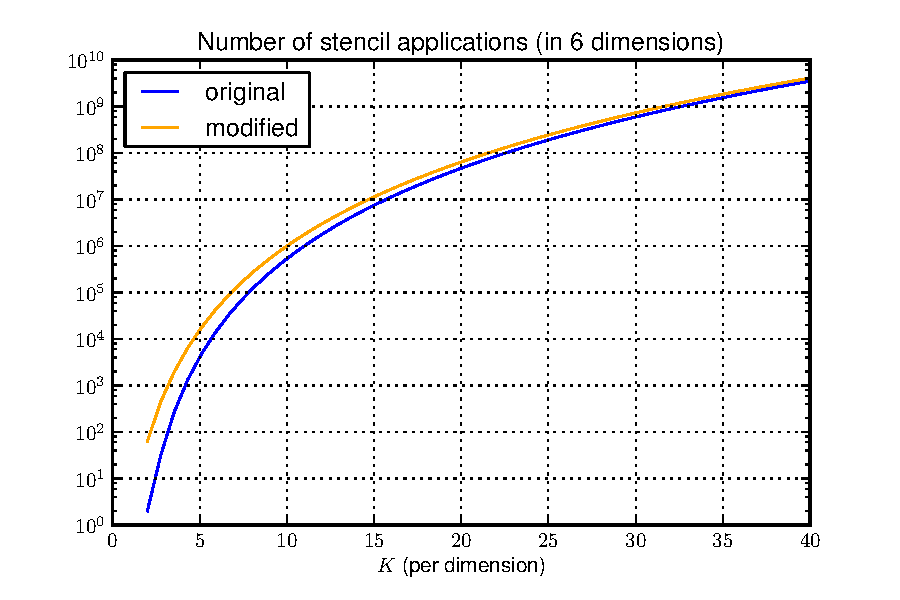
\includegraphics[scale=0.5]{./fig/number_stencil_applications.pdf}
  \caption{Total number of stencil applications for a hypercubic basis shape
           in $D=6$ dimensions and with $K$ nodes along each direction.}
  \label{fig:number_stencil_applications}
\end{figure}


\subsection{Cost of a stencil application}


We define the cost of a stencil application $\mathcal{S} \phi_{\vec{k}}$ as the
number of multiplications which involve a $\phi$. The reason is that we will
evaluate $\phi_{\vec{k}}$ on large grids with many nodes hence $\phi_{\vec{k}}$
is a very long vector.

During the application of the full stencil $\mathcal{S}^D$ we multiply a
$D$ vector by $\phi$ in the first term. In the second one we multiply
a $D \times D$ matrix by a vector of size $D$ containing a (different) $\phi$
in each element. Hence the application $\mathcal{S}^D \phi_k$ has a total cost
of $D^2+D$.

For the modified stencil we only evaluate the first element of the vector equation
and therefore we compute the product of a scalar with $\phi$ and form an inner
product between two vectors of length $D$, one containing a (different) $\phi$
in each element. The application of any modified stencil $\mathcal{S}^D_d$ has
therefore a total cost of $D+1$ which is linear in the number of dimensions.
Figure \ref{fig:cost_stencil_application} shows the cost of both stencils
as a function of dimension $D$.

\begin{figure}
  \centering
  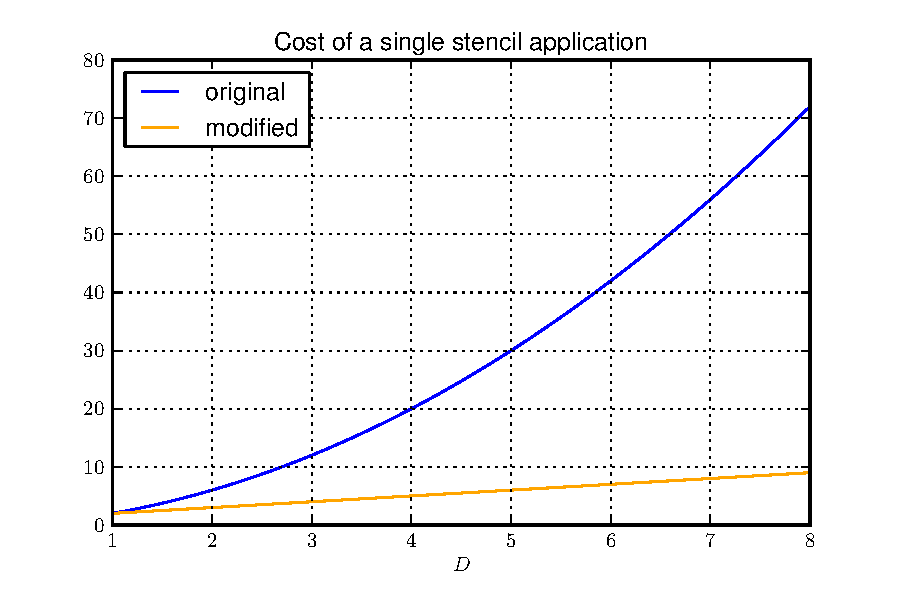
\includegraphics[scale=0.5]{./fig/cost_stencil_application.pdf}
  \caption{The costs of both stencil types in several dimensions.}
  \label{fig:cost_stencil_application}
\end{figure}

If we now compare both evaluation schemes by the number of stencil applications
and the costs of a single application it turns out that the scheme using modified
stencils is much more efficient! In formal notation we find:

\begin{equation*}
  \left(\prod_{d=0}^{D-1} (K_d -1) +1\right) (D^2+D) < \left(\prod_{d=0}^{D-1} K_d -1\right) (D+1)
\end{equation*}

for large enough $K$ where the cross over point depends on the dimension $D$.
For $D = 1$ both schemes are equivalent and have the same costs. Figure
\ref{fig:total_cost_evaluation} shows the overall costs for an hypercubic
basis shape in $D=6$ dimensions.

\begin{figure}
  \centering
  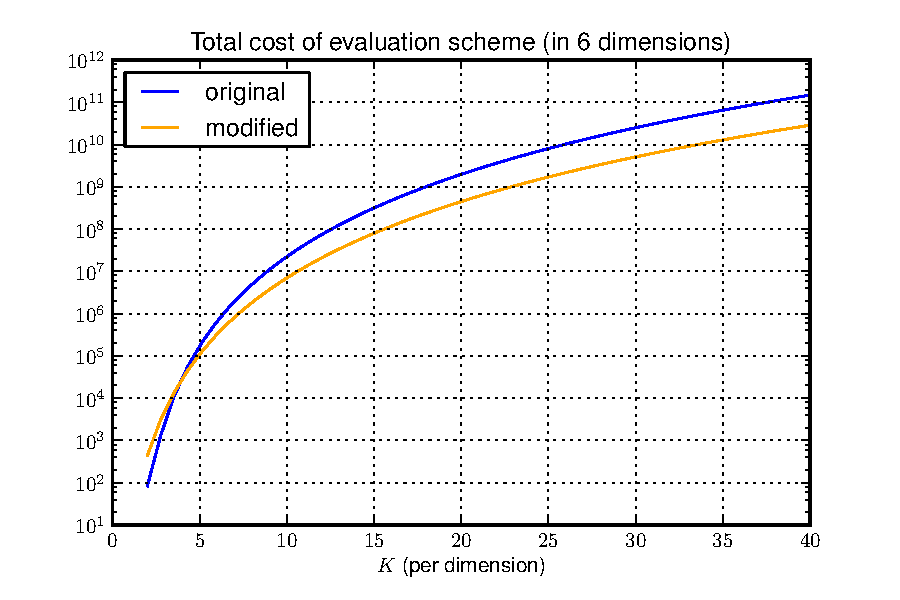
\includegraphics[scale=0.5]{./fig/total_cost_evaluation.pdf}
  \caption{Total cost of a basis evaluation for a hypercubic basis shape
           in $D=6$ dimensions and with $K$ nodes along each direction.}
  \label{fig:total_cost_evaluation}
\end{figure}


\section{Vector-valued wavepackets}


For the purpose of solving the time-dependent Schrödinger equation with non-adiabatic
potentials the scalar wavepackets are not enough. Recall that the potential has $N$
different energy levels. The wavefunction $\Ket{\varphi}$ needs therefore $N$ components
stacked into a vector. In the following we construct \emph{vectorial wavepackets}
where each component is given by a scalar wavepacket. Formally we are in this situation:

\begin{equation}
  \Psi(\vec{x}, t) \assign
  \begin{pmatrix}
    \Phi_0(\vec{x}, t) \\
    \vdots \\
    \Phi_{N-1}(\vec{x}, t)
  \end{pmatrix} \,.
\end{equation}

How many free input parameters does this object have? Each component $\Phi_i$ needs
a set $\Pi_i$ of Hagedorn parameters. (We should write $\Phi_i\left[\Pi_i\right]$
but this becomes lengthy so we drop this soon.) If we use the very same parameter
set $\Pi$ for each component we arrive at what we call a \emph{homogeneous wavepacket}.

\begin{definition}[Homogeneous vectorial wavepacket]
  \begin{equation} \label{eq:vectorial_wavepacket_hom}
    \Ket{\Psi} \assign
    \Psi\left[\Pi\right](\vec{x}, t)
    =
    \begin{pmatrix}
      \Phi_0\left[\Pi\right](\vec{x}, t) \\
      \vdots \\
      \Phi_{N-1}\left[\Pi\right](\vec{x}, t) \\
    \end{pmatrix}
  \end{equation}
  where $\Pi_i \equiv \Pi_j \equiv \Pi \,\forall\, i,j$
\end{definition}

However, at any fixed time each component is independent from all other ones. For
this reason we can choose possibly different sets $\Pi_i$ of parameters for all
$N$ components. By doing this we get an \emph{inhomogeneous wavepacket}, formally
defined as:

\begin{definition}[Inhomogeneous vectorial wavepacket]
  \begin{equation} \label{eq:vectorial_wavepacket_inhom}
    \Ket{\Psi} \assign
    \Psi\left[\Pi_0, \ldots, \Pi_{N-1}\right](\vec{x}, t)
    =
    \begin{pmatrix}
      \Phi_0\left[\Pi_0\right](\vec{x}, t) \\
      \vdots \\
      \Phi_{N-1}\left[\Pi_{N-1}\right](\vec{x}, t) \\
    \end{pmatrix}
  \end{equation}
  where $\Pi_i \neq \Pi_j$ is possible.
\end{definition}

In some applications, for example the spawning approach applied to tunneling
\cite{Gradinaru_semiclassical_tunneling} and the non-adiabatic case
\cite{B_spawning_thesis}, it perfectly makes sense to expand every component
into a different basis of $L^2\left(\mathbb{R}^D\right)$. And since each basis
$\phi_{\vec{k}}$ is essentially fully determined by the parameter set $\Pi$ of
its basis functions $\phi_{\vec{k}}$, this results in different parameter sets
$\Pi_i$ for each component $\Phi_i$.

For some computations we find a more explicit representation of $\Psi$ to be
of greater use. The above definitions can be trivially rewritten as follows by
introducing the unit vectors $\vec{e}^j$ of the canonical basis of $\mathbb{R}^N$.
In the homogeneous case we get:

\begin{equation}
  \Psi\left[\Pi\right](\vec{x}, t) = \sum_{n=0}^{N-1} \vec{e}^n \Phi_n\left[\Pi\right](\vec{x}, t)
\end{equation}

and in the inhomogeneous one:

\begin{equation}
  \Psi\left[\Pi_0,\ldots,\Pi_{N-1}\right](\vec{x}, t) = \sum_{n=0}^{N-1} \vec{e}^n \Phi_n\left[\Pi_n\right](\vec{x}, t) \,.
\end{equation}

We should also note that each component can have an individual basis shape $\mathfrak{K}_n$.
But from now on we will not mention this too often but implicitly assume that each
scalar wavepacket uses the currently best basis shape whatever that means.


\section{Gradient computation}
\label{sec:gradient_computation}


In this section we want to compute the gradient of a scalar wavepacket $\Phi$. More precisely
we find the result of the operator application $-i \varepsilon^2 \nabla \Phi$. From
now on we define the short hand notation $y \assign -i \varepsilon^2 \nabla$. We would
like to have an explicit representation of $y$. Of course it includes just the ordinary
gradient differential operator. But we need a more involved representation allowing us to
easily compute the application of $y$ to a wavepacket of the form given in \eqref{eq:scalar_wavepacket}.
Luckily there is a term of precisely the form of $y$ included in the definition of the
ladder operators in equation \eqref{eq:raising_ops_Dd_explicit}. We proceed by solving the
linear system consisting of the two operator definitions of $\mathcal{L}$ and $\mathcal{R}$
for $y$. We begin by transforming the definition of $\mathcal{R}$ as follows (with the usual
definition of $\theta$):

\begin{align*}
  \mathcal{R} & =  \frac{i}{\sqrt{2\varepsilon^2}} \left( \mat{P}\H (\vec{x}-\vec{q}) - \mat{Q}\H (\vec{y}-\vec{p}) \right) \\
  \mathcal{R} & = \theta \mat{P}\H (\vec{x}-\vec{q}) - \theta \mat{Q}\H (\vec{y}-\vec{p}) \\
  \theta \mat{Q}\H (\vec{y}-\vec{p}) & = -\mathcal{R} + \theta \mat{P}\H (\vec{x}-\vec{q}) \\
  \mat{Q}\H (\vec{y}-\vec{p}) & = -\frac{1}{\theta} \mathcal{R} + \mat{P}\H (\vec{x}-\vec{q}) \,.
\end{align*}

Before we proceed in solving this for $y$ we transform the definition of $\mathcal{L}$
such that we can replace the term $(\vec{x}-\vec{q})$:

\begin{align*}
  \mathcal{L} & = -\theta \mat{P}\T (\vec{x}-\vec{q}) + \theta \mat{Q}\T (\vec{y}-\vec{p}) \\
  \theta \mat{P}\T (\vec{x}-\vec{q}) & = -\mathcal{L} + \theta \mat{Q}\T (\vec{y}-\vec{p}) \\
  \mat{P}\T (\vec{x}-\vec{q}) & = -\frac{1}{\theta}\mathcal{L} + \mat{Q}\T (\vec{y}-\vec{p}) \\
  \vec{x}-\vec{q} & = -\frac{1}{\theta}\mat{P}\Tinv\mathcal{L} + \mat{P}\Tinv\mat{Q}\T (\vec{y}-\vec{p}) \,.
\end{align*}

Then we can plug this into the above equation:

\begin{align*}
  \mat{Q}\H (\vec{y}-\vec{p}) & = -\frac{1}{\theta} \mathcal{R} +
                                  \mat{P}\H \left(-\frac{1}{\theta}\mat{P}\Tinv\mathcal{L} + \mat{P}\Tinv\mat{Q}\T (\vec{y}-\vec{p}) \right) \\
  \mat{Q}\H (\vec{y}-\vec{p}) & = -\frac{1}{\theta} \mathcal{R} +
                                  -\frac{1}{\theta} \mat{P}\H\mat{P}\Tinv\mathcal{L}
                                  +\mat{P}\H\mat{P}\Tinv\mat{Q}\T (\vec{y}-\vec{p}) \\
  \mat{Q}\H \vec{y} - \mat{Q}\H\vec{p} & = -\frac{1}{\theta} \mathcal{R}
                                           -\frac{1}{\theta} \mat{P}\H\mat{P}\Tinv\mathcal{L}
                                           +\mat{P}\H\mat{P}\Tinv\mat{Q}\T \vec{y}
                                           -\mat{P}\H\mat{P}\Tinv\mat{Q}\T\vec{p} \\
  \mat{Q}\H \vec{y} - \mat{P}\H\mat{P}\Tinv\mat{Q}\T \vec{y}
   & = -\frac{1}{\theta} \mathcal{R}
       -\frac{1}{\theta} \mat{P}\H\mat{P}\Tinv\mathcal{L}
       +\mat{Q}\H\vec{p}
       -\mat{P}\H\mat{P}\Tinv\mat{Q}\T\vec{p} \\
  \underbrace{\left(\mat{Q}\H - \mat{P}\H\mat{P}\Tinv\mat{Q}\T\right)}_{**} \vec{y}
   & = -\frac{1}{\theta} \mathcal{R}
       -\frac{1}{\theta} \mat{P}\H\mat{P}\Tinv\mathcal{L}
       +\left(\mat{Q}\H - \mat{P}\H\mat{P}\Tinv\mat{Q}\T\right)\vec{p} \,.
\end{align*}

Our next task is the computation of the subexpression $**$. For this we start again
with the basis relations from \eqref{eq:PQcond_Dd}. For the first one we get:

\begin{align*}
  \mat{Q}\H \mat{P} - \mat{P}\H \mat{Q} & = 2i \id \\
  \mat{Q}\H - \mat{P}\H \mat{Q} \mat{P}\inv & = 2i \mat{P}\inv \\
\end{align*}

and from the second one:

\begin{align*}
  \mat{P}\T \mat{Q} - \mat{Q}\T \mat{P} & = 0 \\
  \mat{Q} - \mat{P}\Tinv \mat{Q}\T \mat{P} & = 0 \\
  \mat{Q} & = \mat{P}\Tinv \mat{Q}\T \mat{P} \,.
\end{align*}

Combining these two results (replacing the second $\mat{Q}$) we obtain:

\begin{align*}
  \mat{Q}\H - \mat{P}\H \mat{P}\Tinv \mat{Q}\T \mat{P} \mat{P}\inv & = 2i \mat{P}\inv \\
  \mat{Q}\H - \mat{P}\H \mat{P}\Tinv \mat{Q}\T & = 2i \mat{P}\inv \,.
\end{align*}

This last line can then be used as a substitution for $**$ above:

\begin{align*}
  2i \mat{P}\inv \vec{y} & = -\frac{1}{\theta} \mathcal{R}
                             -\frac{1}{\theta} \mat{P}\H\mat{P}\Tinv\mathcal{L}
                             +2i \mat{P}\inv \vec{p} \\
  \mat{P}\inv \vec{y} & = -\frac{1}{2i\theta} \mathcal{R}
                          -\frac{1}{2i\theta} \mat{P}\H \mat{P}\Tinv \mathcal{L}
                          +\mat{P}\inv \vec{p} \\
  \vec{y} & = -\frac{1}{2i\theta} \mat{P}\mathcal{R}
                          -\frac{1}{2i\theta} \mat{P} \mat{P}\H \mat{P}\Tinv \mathcal{L}
                          +\vec{p} \,.
\end{align*}

Finally cleaning up and undoing the introduction of $\theta$ we arrive at:

\begin{equation}
  \vec{y} = \sqrt{\frac{\varepsilon^2}{2}} \left( \mat{P}\mathcal{R} + \mat{\conj{P}} \mathcal{L} \right) + \vec{p} \,.
\end{equation}

If we had begun by using the operators $\mathcal{L}$ and $\mathcal{R}$ in the opposite order
we would have got the complex conjugate equation:

\begin{equation}
  \vec{y} = \sqrt{\frac{\varepsilon^2}{2}} \left( \conj{\mat{P}}\mathcal{L} + \mat{P} \mathcal{R} \right) + \vec{p} \,.
\end{equation}

We can simplify the matrix product $\mat{P} \mat{P}\H \mat{P}\Tinv$ to obtain $\mat{\conj{P}}$.
The reason is the conditions \eqref{eq:PQcond_Dd} which must be fulfilled by
$\mat{P}$ and $\mat{Q}$, see \cite{H_ladder_operators}.


\subsection{Applying the gradient operator}


With this explicit representation of the $y$ operator in terms of raising
and lowering operators we can now study its application to an arbitrary
basis function $\phi_{\vec{k}}$. In the end we then need to apply $y$ to the
whole scalar wavepacket $\Phi$ in order to find its kinetic energy.

What do we have to expect when applying $y$ to a basis function $\phi_{\vec{k}}$?
First, we know that the gradient is defined as usual as:

\begin{equation*}
  \nabla_{\vec{x}} \assign
  \begin{pmatrix}
    \pdiff{}{x_0} \\
    \vdots \\
    \pdiff{}{x_{D-1}} \\
  \end{pmatrix} \,.
\end{equation*}

Hence we have to expect that the gradient applied to $\phi_{\vec{k}}:\mathbb{R}^D\rightarrow\mathbb{C}$
is a vector with $D$ components. Next we conclude from \eqref{eq:raising_ops_Dd_vectorial} that the
ladder operators applied to a function give another vector of same shape. We wish to compute:

\begin{equation*}
  y \phi_{\vec{k}}(\vec{x}) = \sqrt{\frac{\varepsilon^2}{2}} \left( \mat{P}\mathcal{R} + \conj{\mat{P}} \mathcal{L} \right) \phi_{\vec{k}}(\vec{x})
                              + \vec{p} \phi_{\vec{k}}(\vec{x})
\end{equation*}

and if we carry out the application of the ladder operators we get step by step
the following relation for the gradient of a single basis function:

\begin{equation*}
  y \phi_{\vec{k}}(\vec{x}) =
  \sqrt{\frac{\varepsilon^2}{2}} \left(
  \mat{P}
    \begin{pmatrix}
      \mathcal{R}_0 \\
      \vdots \\
      \mathcal{R}_{D-1}
    \end{pmatrix}
  + \conj{\mat{P}}
    \begin{pmatrix}
      \mathcal{L}_0 \\
      \vdots \\
      \mathcal{L}_{D-1}
    \end{pmatrix}
  \right) \phi_{\vec{k}}(\vec{x})
  + \vec{p} \phi_{\vec{k}}(\vec{x})
\end{equation*}

where we apply the ladder operators now:

\begin{equation} \label{eq:grad_basis_function_DD}
  y \phi_{\vec{k}}(\vec{x})
  =
  \sqrt{\frac{\varepsilon^2}{2}}
  \left(
    \mat{P}
    \begin{pmatrix}
      \sqrt{k_0 + 1} \phi_{\vec{k}+\vec{e}^0} \\
      \vdots \\
      \sqrt{k_{D-1} + 1} \phi_{\vec{k}+\vec{e}^{D-1}}
    \end{pmatrix}
    +
    \conj{\mat{P}}
    \begin{pmatrix}
      \sqrt{k_0} \phi_{\vec{k}-\vec{e}^0} \\
      \vdots \\
      \sqrt{k_{D-1}} \phi_{\vec{k}-\vec{e}^{D-1}}
    \end{pmatrix}
  \right)
  + \vec{p} \phi_{\vec{k}} \,.
\end{equation}

This is just for one single basis function. But we need more.
Thus we compute the gradient of a whole scalar wavepacket
$\Phi = \sum_{\vec{k}\in\mathfrak{K}} c_{\vec{k}}\phi_{\vec{k}}$:

\begin{equation*}
  y \Phi
  = \sum_{\vec{k}\in\mathfrak{K}} y \, c_{\vec{k}}\phi_{\vec{k}}
  = \sum_{\vec{k}\in\mathfrak{K}} c_{\vec{k}} \, y \phi_{\vec{k}}
\end{equation*}

For a shorter notation we define the following variables:

\begin{align*}
  \theta & \assign \sqrt{\frac{\varepsilon^2}{2}} \\
  \vec{\alpha}(\phi_{\vec{k}}) & \assign
     \begin{pmatrix}
      \sqrt{k_0 + 1} \phi_{\vec{k}+\vec{e}^0} \\
      \vdots \\
      \sqrt{k_{D-1} + 1} \phi_{\vec{k}+\vec{e}^{D-1}}
    \end{pmatrix} \\
  \vec{\beta}(\phi_{\vec{k}}) & \assign
    \begin{pmatrix}
      \sqrt{k_0} \phi_{\vec{k}-\vec{e}^0} \\
      \vdots \\
      \sqrt{k_{D-1}} \phi_{\vec{k}-\vec{e}^{D-1}}
    \end{pmatrix} \,.
\end{align*}

Continuing we derive:

\begin{align*}
  & = \sum_{\vec{k}\in\mathfrak{K}}
        \left(
          c_{\vec{k}} \vec{p} \phi_{\vec{k}}
          + \theta c_{\vec{k}} \mat{P} \vec{\alpha}(\phi_{\vec{k}})
          + \theta c_{\vec{k}} \conj{\mat{P}} \vec{\beta}(\phi_{\vec{k}})
        \right) \nonumber\\
  & = \sum_{\vec{k}\in\mathfrak{K}} c_{\vec{k}} \vec{p} \phi_{\vec{k}}
    + \sum_{\vec{k}\in\mathfrak{K}} \theta c_{\vec{k}} \mat{P} \vec{\alpha}(\phi_{\vec{k}})
    + \sum_{\vec{k}\in\mathfrak{K}} \theta c_{\vec{k}} \conj{\mat{P}} \vec{\beta}(\phi_{\vec{k}}) \,.
\end{align*}

It becomes obvious that $y \phi_{\vec{k}}$ has contributions from all neighbours
$\phi_{\vec{k} + \vec{e}^d}$ and $\phi_{\vec{k} - \vec{e}^d}$ for all $d \in [0, \ldots, D-1]$
and from $\phi_{\vec{k}}$. This immediately raises the question of an efficient
computation. In the end we will need $y \phi_{\vec{k}}$ for all $\vec{k} \in \mathfrak{K}$.
Since there are ladder operators involved we have to be careful for all $\vec{k}$
on the border of $\mathfrak{K}$ who don't have a full set of neighbours in all
directions $d$. For each neighbour $\vec{k}\pm\vec{e}^d$ that is not part of the
basis shape $\mathfrak{K}$ we have to decide what to do. And the rules are as follows.

If the vector $\vec{k}-\vec{e}^d$ has negative components, then we can take the
corresponding basis function to be equivalent zero. We call this situation an
\emph{underflow} \footnote{ This has nothing to do with the usual arithmetic
over/underflow. It just serves as a notation of \emph{where} we access elements
outside of our basis shape $\mathfrak{K}$.}.

The other case is more involved. The functions $\phi_{\vec{k}}$ clearly never
vanish identically zero. However we only have finite linear combinations $\Phi$ of
basis functions $\phi_{\vec{k}}$. Hence all coefficients for sufficiently \emph{large}
$\vec{k}$ vanish. And finally we are only interested in the new coefficients
$c_{\vec{k}}^{\prime i}$ of each component $i$ of the gradient $y \phi_{\vec{k}}$. For
this reason we can also insert zeros in the case such an \emph{overflow} occurs.
For an example of the situation and the issues that may arise refer to figure
\ref{fig:grad_phi_kl_stencil}.

\begin{figure}
  \centering
  \begin{tikzpicture}[%
    func/.style={scale=0.8,color=gray},
    zero/.style={scale=0.8,color=gray}]

    \node[zero, color=black] (v0m1) at (1,0) {$0$};
    \node[zero] (v1m1) at (2,0) {$0$};
    \node[zero] (v2m1) at (3,0) {$0$};
    \node[zero] (v3m1) at (4,0) {$0$};
    \node[zero] (v4m1) at (5,0) {$0$};
    \node[zero] (v5m1) at (6,0) {$0$};
    %\node[zero] (v6m1) at (7,0) {$0$};

    \node[zero, color=black] (vm10) at (0,1) {$0$};
    \node[zero] (vm11) at (0,2) {$0$};
    \node[zero] (vm12) at (0,3) {$0$};
    \node[zero] (vm13) at (0,4) {$0$};
    \node[zero, color=black] (vm14) at (0,5) {$0$};
    %\node[zero] (vm15) at (0,6) {$0$};

    \node[func, color=black] (v00) at (1,1) {$\phi_{0,0}$};
    \node[func, color=black] (v01) at (1,2) {$\phi_{0,1}$};
    \node[func] (v02) at (1,3) {$\phi_{0,2}$};
    \node[func, color=black] (v03) at (1,4) {$\phi_{0,3}$};
    \node[func, color=black] (v04) at (1,5) {$\phi_{0,4}$};
    \node[func, color=black] (v05) at (1,6) {$\phi_{0,5}$};

    \node[func, color=black] (v10) at (2,1) {$\phi_{1,0}$};
    \node[func] (v11) at (2,2) {$\phi_{1,1}$};
    \node[func] (v12) at (2,3) {$\phi_{1,2}$};
    \node[func] (v13) at (2,4) {$\phi_{1,3}$};
    \node[func, color=black] (v14) at (2,5) {$\phi_{1,4}$};
    \node[func] (v15) at (2,6) {$\phi_{1,5}$};

    \node[func] (v20) at (3,1) {$\phi_{2,0}$};
    \node[func] (v21) at (3,2) {$\phi_{2,1}$};
    \node[func, color=black] (v22) at (3,3) {$\phi_{2,2}$};
    \node[func] (v23) at (3,4) {$\phi_{2,3}$};
    \node[func] (v24) at (3,5) {$\phi_{2,4}$};
    \node[func] (v25) at (3,6) {$\phi_{2,5}$};

    \node[func] (v30) at (4,1) {$\phi_{3,0}$};
    \node[func, color=black] (v31) at (4,2) {$\phi_{3,1}$};
    \node[func, color=black] (v32) at (4,3) {$\phi_{3,2}$};
    \node[func, color=black] (v33) at (4,4) {$\phi_{3,3}$};
    \node[func] (v34) at (4,5) {$\phi_{3,4}$};
    \node[func] (v35) at (4,6) {$\phi_{3,5}$};

    \node[func] (v40) at (5,1) {$\phi_{4,0}$};
    \node[func] (v41) at (5,2) {$\phi_{4,1}$};
    \node[func, color=black] (v42) at (5,3) {$\phi_{4,2}$};
    \node[func] (v43) at (5,4) {$\phi_{4,3}$};
    \node[func, color=black] (v44) at (5,5) {$\phi_{4,4}$};
    \node[func] (v45) at (5,6) {$\phi_{4,5}$};

    \node[func] (v50) at (6,1) {$\phi_{5,0}$};
    \node[func] (v51) at (6,2) {$\phi_{5,1}$};
    \node[func] (v52) at (6,3) {$\phi_{5,2}$};
    \node[func, color=black] (v53) at (6,4) {$\phi_{5,3}$};
    \node[func, color=black] (v54) at (6,5) {$\phi_{5,4}$};
    \node[func, color=black] (v55) at (6,6) {$\phi_{5,5}$};

    \node[func] (v60) at (7,1) {$\phi_{6,0}$};
    \node[func] (v61) at (7,2) {$\phi_{6,1}$};
    \node[func] (v62) at (7,3) {$\phi_{6,2}$};
    \node[func] (v63) at (7,4) {$\phi_{6,3}$};
    \node[func, color=black] (v64) at (7,5) {$\phi_{6,4}$};
    %\node[func] (v65) at (7,6) {$\phi_{6,5}$};

    \begin{scope}
    \draw[draw=black,line width=0.7pt] ($(v00)+(0.0,-0.5)$)
        to[out=0,in=180] ($(v50)+(0.0,-0.5)$)
        to[out=0,in=270] ($(v50)+(0.5,0.0)$)
        to[out=90,in=270] ($(v54)+(0.5,0.0)$)
        to[out=90,in=0] ($(v54)+(0.0,0.5)$)
        to[out=180,in=0] ($(v04)+(0.0,0.5)$)
        to[out=180,in=90] ($(v04)+(-0.5,0.0)$)
        to[out=270,in=90] ($(v00)+(-0.5,0.0)$)
        to[out=270,in=180] ($(v00)+(0.0,-0.5)$);
    \end{scope}

    % lower left
    \begin{scope}
    \draw[draw=blue!100,line width=0.8pt] ($(vm10)+(0.0,0.3)$)
        to[out=170,in=90] ($(vm10)+(-0.3,0.0)$)
        to[out=270,in=190] ($(vm10)+(0.0,-0.3)$)
        to[out=10,in=80] ($(v0m1)+(-0.3,0.0)$)
        to[out=260,in=180] ($(v0m1)+(0.0,-0.3)$)
        to[out=0,in=280] ($(v0m1)+(0.3,0.0)$)
        to[out=100,in=350] ($(vm10)+(0.0,0.3)$);
    \end{scope}
    \begin{scope}
    \draw[draw=orange!100,line width=0.8pt] ($(v10)-(0.0,0.3)$)
        to[out=10,in=170] ($(v10)-(0.0,0.3)$)
        to[out=0,in=270] ($(v10)-(-0.3,0.0)$)
        to[out=90,in=10] ($(v10)-(0.0,-0.3)$)
        to[out=190,in=260] ($(v01)-(-0.3,0.0)$)
        to[out=80,in=0] ($(v01)-(0.0,-0.3)$)
        to[out=180,in=100] ($(v01)-(0.3,0.0)$)
        to[out=280,in=170] ($(v10)-(0.0,0.3)$);
    \end{scope}
    \begin{scope}
    \draw[draw=gray!100,line width=0.8pt] ($(v00)-(0.0,0.3)$)
        to[out=180,in=270] ($(v00)-(0.3,0.0)$)
        to[out=90,in=180] ($(v00)+(0.0,0.3)$)
        to[out=0,in=90] ($(v00)+(0.3,0.0)$)
        to[out=270,in=0] ($(v00)-(0.0,0.3)$);
    \end{scope}

    % upper left
    \begin{scope}
    \draw[draw=blue!100,line width=0.8pt] ($(vm14)+(0.0,0.3)$)
        to[out=170,in=90] ($(vm14)+(-0.3,0.0)$)
        to[out=270,in=190] ($(vm14)+(0.0,-0.3)$)
        to[out=10,in=80] ($(v03)+(-0.3,0.0)$)
        to[out=260,in=180] ($(v03)+(0.0,-0.3)$)
        to[out=0,in=280] ($(v03)+(0.3,0.0)$)
        to[out=100,in=350] ($(vm14)+(0.0,0.3)$);
    \end{scope}
    \begin{scope}
    \draw[draw=orange!100,line width=0.8pt] ($(v14)-(0.0,0.3)$)
        to[out=10,in=170] ($(v14)-(0.0,0.3)$)
        to[out=0,in=270] ($(v14)-(-0.3,0.0)$)
        to[out=90,in=10] ($(v14)-(0.0,-0.3)$)
        to[out=190,in=260] ($(v05)-(-0.3,0.0)$)
        to[out=80,in=0] ($(v05)-(0.0,-0.3)$)
        to[out=180,in=100] ($(v05)-(0.3,0.0)$)
        to[out=280,in=170] ($(v14)-(0.0,0.3)$);
    \end{scope}
    \begin{scope}
    \draw[draw=gray!100,line width=0.8pt] ($(v04)-(0.0,0.3)$)
        to[out=180,in=270] ($(v04)-(0.3,0.0)$)
        to[out=90,in=180] ($(v04)+(0.0,0.3)$)
        to[out=0,in=90] ($(v04)+(0.3,0.0)$)
        to[out=270,in=0] ($(v04)-(0.0,0.3)$);
    \end{scope}

    % upper right
    \begin{scope}
    \draw[draw=blue!100,line width=0.8pt] ($(v44)+(0.0,0.3)$)
        to[out=170,in=90] ($(v44)+(-0.3,0.0)$)
        to[out=270,in=190] ($(v44)+(0.0,-0.3)$)
        to[out=10,in=80] ($(v53)+(-0.3,0.0)$)
        to[out=260,in=180] ($(v53)+(0.0,-0.3)$)
        to[out=0,in=280] ($(v53)+(0.3,0.0)$)
        to[out=100,in=350] ($(v44)+(0.0,0.3)$);
    \end{scope}
    \begin{scope}
    \draw[draw=orange!100,line width=0.8pt] ($(v64)-(0.0,0.3)$)
        to[out=10,in=170] ($(v64)-(0.0,0.3)$)
        to[out=0,in=270] ($(v64)-(-0.3,0.0)$)
        to[out=90,in=10] ($(v64)-(0.0,-0.3)$)
        to[out=190,in=260] ($(v55)-(-0.3,0.0)$)
        to[out=80,in=0] ($(v55)-(0.0,-0.3)$)
        to[out=180,in=100] ($(v55)-(0.3,0.0)$)
        to[out=280,in=170] ($(v64)-(0.0,0.3)$);
    \end{scope}
    \begin{scope}
    \draw[draw=gray!100,line width=0.8pt] ($(v54)-(0.0,0.3)$)
        to[out=180,in=270] ($(v54)-(0.3,0.0)$)
        to[out=90,in=180] ($(v54)+(0.0,0.3)$)
        to[out=0,in=90] ($(v54)+(0.3,0.0)$)
        to[out=270,in=0] ($(v54)-(0.0,0.3)$);
    \end{scope}

    % central
    \begin{scope}
    \draw[draw=blue!100,line width=0.8pt] ($(v22)+(0.0,0.3)$)
        to[out=170,in=90] ($(v22)+(-0.3,0.0)$)
        to[out=270,in=190] ($(v22)+(0.0,-0.3)$)
        to[out=10,in=80] ($(v31)+(-0.3,0.0)$)
        to[out=260,in=180] ($(v31)+(0.0,-0.3)$)
        to[out=0,in=280] ($(v31)+(0.3,0.0)$)
        to[out=100,in=350] ($(v22)+(0.0,0.3)$);
    \end{scope}
    \begin{scope}
    \draw[draw=orange!100,line width=0.8pt] ($(v42)-(0.0,0.3)$)
        to[out=10,in=170] ($(v42)-(0.0,0.3)$)
        to[out=0,in=270] ($(v42)-(-0.3,0.0)$)
        to[out=90,in=10] ($(v42)-(0.0,-0.3)$)
        to[out=190,in=260] ($(v33)-(-0.3,0.0)$)
        to[out=80,in=0] ($(v33)-(0.0,-0.3)$)
        to[out=180,in=100] ($(v33)-(0.3,0.0)$)
        to[out=280,in=170] ($(v42)-(0.0,0.3)$);
    \end{scope}
    \begin{scope}
    \draw[draw=gray!100,line width=0.8pt] ($(v32)-(0.0,0.3)$)
        to[out=180,in=270] ($(v32)-(0.3,0.0)$)
        to[out=90,in=180] ($(v32)+(0.0,0.3)$)
        to[out=0,in=90] ($(v32)+(0.3,0.0)$)
        to[out=270,in=0] ($(v32)-(0.0,0.3)$);
    \end{scope}
\end{tikzpicture}

  \caption[Computing the gradient in two dimensions] {Stencil application for
           computing the gradient $y \phi_{\vec{k}}$ for different $\vec{k}$ in
           two dimensions. For each computation we need the function itself
           (grey circles), the backward neighbours $\phi_{\vec{k}-\vec{e}^d}$
           (blue contours) and the forward neighbours $\phi_{\vec{k}+\vec{e}^d}$
           (orange contours). Clearly we need additional functions outside of
           the basis shape $\mathfrak{K}$ (black rectangle). In all corners
            and along all sides we under- and overflow respectively.}
  \label{fig:grad_phi_kl_stencil}
\end{figure}

Before we continue let's make a not so small but very simple example. Assume
the hypercubic basis shape in two dimensions is $\mathfrak{K} = \vec{K} = (3,3)$.
The wavepacket consists of the following linear combination:

\begin{align*}
  \Phi \assign \, & c_{0,0} \phi_{0,0} + c_{1,0} \phi_{1,0} + c_{2,0} \phi_{2,0} \\
             + \, & c_{0,1} \phi_{0,1} + c_{1,1} \phi_{1,1} + c_{2,1} \phi_{2,1} \\
             + \, & c_{0,2} \phi_{0,2} + c_{1,2} \phi_{1,2} + c_{2,2} \phi_{2,2} \,.
\end{align*}

Computing the gradients individually for some of the terms we get:

\begin{center}
\begin{tabular}{ll}
Multi-index node  & Gradient \\
\hline \\
$\vec{k} = (0,0)$ & $c_{0,0} \, \vec{p} \phi_{0,0} +
                     \theta c_{0,0} \, \mat{P} \begin{pmatrix} \sqrt{1} \, \phi_{1,0} \\
                                                               \sqrt{1} \, \phi_{0,1}
                                               \end{pmatrix} +
                     \theta c_{0,0} \, \conj{\mat{P}} \begin{pmatrix} \sqrt{0} \, \phi_{-1,0} \\
                                                                      \sqrt{0} \, \phi_{0,-1}
                                                      \end{pmatrix}$\\
$\vec{k} = (1,0)$ & $c_{1,0} \, \vec{p} \phi_{1,0} +
                     \theta c_{1,0} \, \mat{P} \begin{pmatrix} \sqrt{2} \, \phi_{2,0} \\
                                                               \sqrt{1} \, \phi_{1,1}
                                               \end{pmatrix} +
                     \theta c_{1,0} \, \conj{\mat{P}} \begin{pmatrix} \sqrt{1} \, \phi_{0,0} \\
                                                                      \sqrt{0} \, \phi_{1,-1}
                                                      \end{pmatrix}$\\
$\vec{k} = (0,1)$ & $c_{0,1} \, \vec{p} \phi_{0,1} +
                     \theta c_{0,1} \, \mat{P} \begin{pmatrix} \sqrt{1} \, \phi_{1,1} \\
                                                               \sqrt{2} \, \phi_{0,2}
                                               \end{pmatrix} +
                     \theta c_{0,1} \, \conj{\mat{P}} \begin{pmatrix} \sqrt{0} \, \phi_{-1,1} \\
                                                                      \sqrt{1} \, \phi_{0,0}
                                                      \end{pmatrix}$\\
$\vec{k} = (1,1)$ & $c_{1,1} \, \vec{p} \phi_{1,1} +
                     \theta c_{1,1} \, \mat{P} \begin{pmatrix} \sqrt{2} \, \phi_{2,1} \\
                                                               \sqrt{2} \, \phi_{1,2}
                                               \end{pmatrix} +
                     \theta c_{1,1} \, \conj{\mat{P}} \begin{pmatrix} \sqrt{1} \, \phi_{0,1} \\
                                                                      \sqrt{1} \, \phi_{1,0}
                                                      \end{pmatrix}$ \\
$\vec{k} = (2,1)$ & $c_{2,1} \, \vec{p} \phi_{2,1} +
                     \theta c_{2,1} \, \mat{P} \begin{pmatrix} \sqrt{3} \, \phi_{3,1} \\
                                                               \sqrt{2} \, \phi_{2,2}
                                               \end{pmatrix} +
                     \theta c_{2,1} \, \conj{\mat{P}} \begin{pmatrix} \sqrt{2} \, \phi_{1,1} \\
                                                                      \sqrt{1} \, \phi_{2,0}
                                                      \end{pmatrix}$ \\
$\vec{k} = (1,2)$ & $c_{1,2} \, \vec{p} \phi_{1,2} +
                     \theta c_{1,2} \, \mat{P} \begin{pmatrix} \sqrt{2} \, \phi_{2,2} \\
                                                               \sqrt{3} \, \phi_{1,3}
                                               \end{pmatrix} +
                     \theta c_{1,2} \, \conj{\mat{P}} \begin{pmatrix} \sqrt{1} \, \phi_{0,2} \\
                                                                      \sqrt{2} \, \phi_{1,1}
                                                      \end{pmatrix}$ \\
$\vdots$ & $\hdots$
\end{tabular}
\end{center}

and we would sum up all these terms to get the overall gradient of $\Phi$. In this form however
it is not of much use to us. We want to represent the gradient again as linear combinations
over the same set of basis functions:

\begin{equation} \label{eq:gradient_basis_expandion}
  y \Phi = \sum_{\vec{k} \in \overline{\mathfrak{K}}} \vec{c}^\prime_{\vec{k}} \phi_{\vec{k}}
\end{equation}

where $\vec{c}^\prime_{\vec{k}} \in \mathbb{C}^{D}$ and $\overline{\mathfrak{K}}$ is the
extended basis shape (in case of our example $\overline{\mathfrak{K}} = \vec{K}^\prime = (4,4)$).
This is indeed possible, expanding the fourth row from the table above in
instances of $\phi_{\vec{k}}$ and summing up we get:

\begin{equation*}
    c_{1,1} \, \vec{p} \phi_{1,1}
  + \theta c_{1,1} \, \sqrt{2} \, \mat{P}_{:,0} \phi_{2,1}
  + \theta c_{1,1} \, \sqrt{2} \, \mat{P}_{:,1} \phi_{1,2}
  + \theta c_{1,1} \, \conj{\mat{P}}_{:,0} \phi_{0,1}
  + \theta c_{1,1} \, \conj{\mat{P}}_{:,1} \phi_{1,0} \,.
\end{equation*}

In finding the coefficient $\vec{c}_{1,1}$ of $\phi_{1,1}$ we have to be very careful, because
there are further terms on up to 4 other rows that contribute to $\vec{c}_{1,1}$.
(Note that this coefficient is a good example as its lattice node has a full set
of 4 neighbours.) Summing up all relevant terms we find that:

\begin{equation*}
  \vec{c}^\prime_{1,1} = c_{1,1} \, \vec{p}
+ \theta c_{0,1} \, \mat{P}_{:,0} \,.
+ \theta c_{1,0} \, \mat{P}_{:,1}
+ \theta c_{2,1} \, \sqrt{2} \, \conj{\mat{P}}_{:,0}
+ \theta c_{1,2} \, \sqrt{2} \, \conj{\mat{P}}_{:,1} \,.
\end{equation*}

The last four terms can be recombined into one per pair and we end up with:

\begin{equation*}
  \vec{c}^\prime_{1,1} = c_{1,1} \, \vec{p}
+ \theta \mat{P}
  \begin{pmatrix}
    c_{0,1} \\ c_{1,0}
  \end{pmatrix}
+ \theta \conj{\mat{P}}
  \begin{pmatrix}
    \sqrt{2} \, c_{2,1} \\ \sqrt{2} \, c_{1,2}
  \end{pmatrix}
\end{equation*}

Doing these transformations in a systematic way is the major issue in computing the gradients.
With a bit of guessing we can find the following general rule for the coefficient vectors
$\vec{c}^\prime_{\vec{k}}$ for all $\vec{k} \in \overline{\mathfrak{K}}$:

\begin{equation*}
  \vec{c}^\prime_{\vec{k}} = c_{\vec{k}} \, \vec{p}
                             + \sqrt{\frac{\varepsilon^2}{2}} \sum_{d=0}^{D-1} c_{\vec{k}+\vec{e}^d} \, \sqrt{\vec{k}_{d}+1} \, \conj{\mat{P}}_{:,d}
                             + \sqrt{\frac{\varepsilon^2}{2}} \sum_{d=0}^{D-1} c_{\vec{k}-\vec{e}^d} \, \sqrt{\vec{k}_{d}} \, \mat{P}_{:,d}
\end{equation*}

which again can be cast in compact form:

\begin{equation} \label{eq:gradient_coefficients_DD}
  \vec{c}^\prime_{\vec{k}} = c_{\vec{k}} \, \vec{p}
                             + \sqrt{\frac{\varepsilon^2}{2}} \left(
                               \conj{\mat{P}}
                               \begin{pmatrix}
                                 c_{\vec{k}+\vec{e}^0} \, \sqrt{\vec{k}_{0}+1} \\
                                 \vdots \\
                                 c_{\vec{k}+\vec{e}^{D-1}} \, \sqrt{\vec{k}_{D-1}+1}
                               \end{pmatrix}
                             + \mat{P}
                               \begin{pmatrix}
                                 c_{\vec{k}-\vec{e}^0} \, \sqrt{\vec{k}_{0}} \\
                                 \vdots \\
                                 c_{\vec{k}-\vec{e}^{D-1}} \, \sqrt{\vec{k}_{D-1}}
                               \end{pmatrix}
                               \right) \,.
\end{equation}


\subsection{Gather-type algorithm}


The most simple algorithm to compute $y \phi_{\vec{k}}$ for all $\vec{k} \in \mathfrak{K}$
has to iterate over all $\vec{k} \in \overline{\mathfrak{K}}$ and apply the
two stencils to get the data from backward and forward neighbours of $\vec{k}$
and to compute $y \phi_{\vec{k}}$ by the formula \eqref{eq:gradient_coefficients_DD}.
This is simple to understand and works reasonably efficient. We call this algorithm the
\emph{gather-type} stencil application.

The only not so easy point here is that we can not iterate just over $\mathfrak{K}$
but have to extend the basis shape due to the nature of the neighbourhood stencil.
In more detail, this is necessary as there are $\vec{k}^\prime \notin \mathfrak{K}$
for which the above formula \eqref{eq:gradient_coefficients_DD} still yields a non-zero result since
the stencil centred at $\vec{k}^\prime$ still overlaps with the basis shape $\mathfrak{K}$.
And we do not want to loose these contributions. Therefore we extend the basis shape
$\mathfrak{K}$ by one node in all directions and get what we denote by $\overline{\mathfrak{K}}$.
This should be clear by looking at figure \ref{fig:grad_phi_kl_stencil}.

In one single space dimension $x$ the gradient equals the derivative and the result
is not a vector of functions but just a function too. Therefore it is easier to
understand the gradient computation for one-dimensional wavepackets $\Phi(x)$ first.
The whole process of the gather-type algorithm is shown in figure
\ref{fig:grad_phi_kl_gather_stencil_1D} in considerable detail.

\begin{figure}
  \centering
  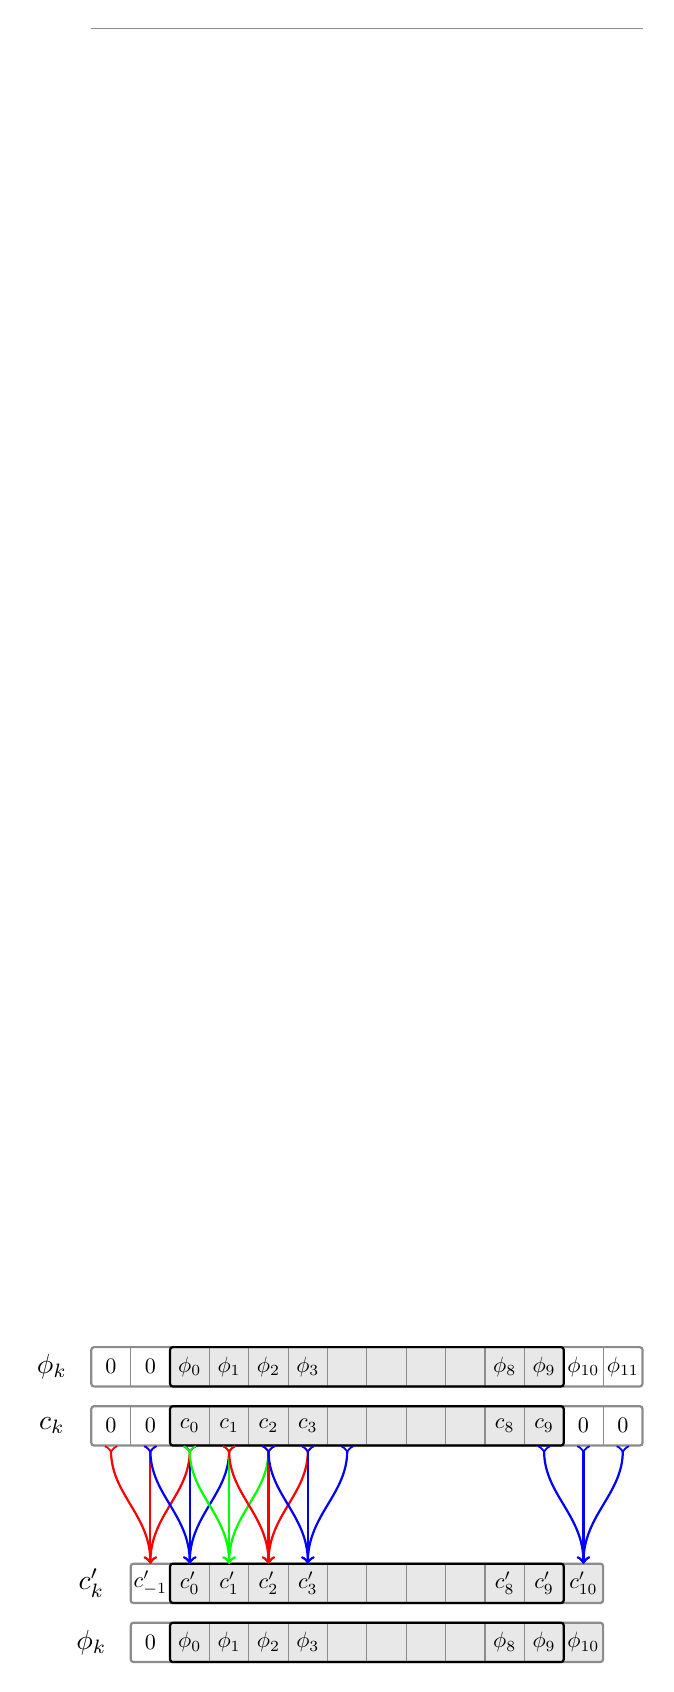
\begin{tikzpicture}
  \coordinate (com2) at (-0.75, 2.0);
  \coordinate (com1) at (-0.25, 2.0);
  \coordinate (co0) at (0.25, 2.0);
  \coordinate (co1) at (0.75, 2.0);
  \coordinate (co2) at (1.25, 2.0);
  \coordinate (co3) at (1.75, 2.0);
  \coordinate (co4) at (2.25, 2.0);
  \coordinate (co5) at (2.75, 2.0);
  \coordinate (co6) at (3.25, 2.0);
  \coordinate (co9) at (4.75, 2.0);
  \coordinate (co10) at (5.25, 2.0);
  \coordinate (co11) at (5.75, 2.0);

  \coordinate (cpm1) at (-0.25, 0.5);
  \coordinate (cp0) at (0.25, 0.5);
  \coordinate (cp1) at (0.75, 0.5);
  \coordinate (cp2) at (1.25, 0.5);
  \coordinate (cp3) at (1.75, 0.5);
  \coordinate (cp4) at (2.25, 0.5);
  \coordinate (cp5) at (2.75, 0.5);
  \coordinate (cp6) at (3.25, 0.5);
  \coordinate (cp8) at (4.25, 0.5);
  \coordinate (cp9) at (4.75, 0.5);
  \coordinate (cp10) at (5.25, 0.5);

  % upper
  \fill[gray!20, rounded corners=1] (0.0,2.75) rectangle (5.0,3.25);
  \draw[step=5mm, ystep=20cm, gray] (-1.0,2.75) grid (6.0,3.25);
  \draw[gray, thick, rounded corners=1] (-1.0,2.75) rectangle (6.0,3.25);
  \draw[black, thick, rounded corners=1] (0.0,2.75) rectangle (5.0,3.25);

  \fill[gray!20, rounded corners=1] (0.0,2.0) rectangle (5.0,2.5);
  \draw[step=5mm, gray] (-1.0,2.0) grid (6.0,2.5);
  \draw[gray, thick, rounded corners=1] (-1.0,2.0) rectangle (6.0,2.5);
  \draw[black, thick, rounded corners=1] (0.0,2.0) rectangle (5.0,2.5);

  % lower
  \fill[gray!20, rounded corners=1] (0.0,-0.75) rectangle (5.5,-0.25);
  \draw[step=5mm, ystep=20cm, gray] (0.0,-0.75) grid (5.0,-0.25);
  \draw[gray, thick, rounded corners=1] (-0.5,-0.75) rectangle (5.5,-0.25);
  \draw[black, thick, rounded corners=1] (0.0,-0.75) rectangle (5.0,-0.25);

  \fill[gray!20, rounded corners=1] (0.0,0.0) rectangle (5.5,0.5);
  \draw[step=5mm, gray] (0.0,0.0) grid (5.0,0.5);
  \draw[gray, thick, rounded corners=1] (-0.5,0.0) rectangle (5.5,0.5);
  \draw[black, thick, rounded corners=1] (0.0,0.0) rectangle (5.0,0.5);

  \draw[>->, thick, color=red] (com2) to[out=270,in=90] (cpm1);
  \draw[>->, thick, color=red] (com1) to[out=270,in=90] (cpm1);
  \draw[>->, thick, color=red] (co0) to[out=270,in=90] (cpm1);

  \draw[>->, thick, color=blue] (com1) to[out=270,in=90] (cp0);
  \draw[>->, thick, color=blue] (co0) to[out=270,in=90] (cp0);
  \draw[>->, thick, color=blue] (co1) to[out=270,in=90] (cp0);

  \draw[>->, thick, color=green] (co0) to[out=270,in=90] (cp1);
  \draw[>->, thick, color=green] (co1) to[out=270,in=90] (cp1);
  \draw[>->, thick, color=green] (co2) to[out=270,in=90] (cp1);

  \draw[>->, thick, color=red] (co1) to[out=270,in=90] (cp2);
  \draw[>->, thick, color=red] (co2) to[out=270,in=90] (cp2);
  \draw[>->, thick, color=red] (co3) to[out=270,in=90] (cp2);

  \draw[>->, thick, color=blue] (co2) to[out=270,in=90] (cp3);
  \draw[>->, thick, color=blue] (co3) to[out=270,in=90] (cp3);
  \draw[>->, thick, color=blue] (co4) to[out=270,in=90] (cp3);

  \draw[>->, thick, color=blue] (co9) to[out=270,in=90] (cp10);
  \draw[>->, thick, color=blue] (co10) to[out=270,in=90] (cp10);
  \draw[>->, thick, color=blue] (co11) to[out=270,in=90] (cp10);

  \node[scale=0.8] at (-0.75,2.25) [black] {$0$};
  \node[scale=0.8] at (-0.25,2.25) [black] {$0$};
  \node[scale=0.8] at (0.25,2.25) [black] {$c_0$};
  \node[scale=0.8] at (0.75,2.25) [black] {$c_1$};
  \node[scale=0.8] at (1.25,2.25) [black] {$c_2$};
  \node[scale=0.8] at (1.75,2.25) [black] {$c_3$};
  \node[scale=0.8] at (4.25,2.25) [black] {$c_8$};
  \node[scale=0.8] at (4.75,2.25) [black] {$c_9$};
  \node[scale=0.8] at (5.25,2.25) [black] {$0$};
  \node[scale=0.8] at (5.75,2.25) [black] {$0$};

  \node[scale=0.8] at (-0.25,0.25) [black] {$c^\prime_{-1}$};
  \node[scale=0.8] at (0.25,0.25) [black] {$c^\prime_0$};
  \node[scale=0.8] at (0.75,0.25) [black] {$c^\prime_1$};
  \node[scale=0.8] at (1.25,0.25) [black] {$c^\prime_2$};
  \node[scale=0.8] at (1.75,0.25) [black] {$c^\prime_3$};
  \node[scale=0.8] at (4.25,0.25) [black] {$c^\prime_8$};
  \node[scale=0.8] at (4.75,0.25) [black] {$c^\prime_9$};
  \node[scale=0.8] at (5.25,0.25) [black] {$c^\prime_{10}$};

  \node[scale=0.8] at (-0.75,3.0) [black] {$0$};
  \node[scale=0.8] at (-0.25,3.0) [black] {$0$};
  \node[scale=0.8] at (0.25,3.0) [black] {$\phi_0$};
  \node[scale=0.8] at (0.75,3.0) [black] {$\phi_1$};
  \node[scale=0.8] at (1.25,3.0) [black] {$\phi_2$};
  \node[scale=0.8] at (1.75,3.0) [black] {$\phi_3$};
  \node[scale=0.8] at (4.25,3.0) [black] {$\phi_8$};
  \node[scale=0.8] at (4.75,3.0) [black] {$\phi_9$};
  \node[scale=0.8] at (5.25,3.0) [black] {$\phi_{10}$};
  \node[scale=0.8] at (5.75,3.0) [black] {$\phi_{11}$};

  \node[scale=0.8] at (-0.25,-0.5) [black] {$0$};
  \node[scale=0.8] at (0.25,-0.5) [black] {$\phi_0$};
  \node[scale=0.8] at (0.75,-0.5) [black] {$\phi_1$};
  \node[scale=0.8] at (1.25,-0.5) [black] {$\phi_2$};
  \node[scale=0.8] at (1.75,-0.5) [black] {$\phi_3$};
  \node[scale=0.8] at (4.25,-0.5) [black] {$\phi_8$};
  \node[scale=0.8] at (4.75,-0.5) [black] {$\phi_9$};
  \node[scale=0.8] at (5.25,-0.5) [black] {$\phi_{10}$};

  \node at (-1.5,3.0) [black] {$\phi_{k}$};
  \node at (-1.0,-0.5) [black] {$\phi_{k}$};
  \node at (-1.5,2.25) [black] {$c_{k}$};
  \node at (-1.0,0.25) [black] {$c^\prime_{k}$};
\end{tikzpicture}

  \caption[Gather-type stencil in 1D] {The gather-type stencil application for
           computing the gradient $y\Phi$. The upper two arrays show the initial linear
           combination $\Phi$ consisting of basis functions $\phi_k$ and coefficients $c_k$.
           The lower two arrays show the linear combination of $\diff{\Phi}{x}$ consisting
           of the same basis functions $\phi_k$ and new coefficients $c_k^\prime$.
           Each of the triple arrows is one single stencil application (formula
           \eqref{eq:gradient_coefficients_DD}), not all applications are shown.
           We see that the basis shape $\overline{\mathfrak{K}}$ for the gradient
           is larger. And also that we access several elements not part of the original
           basis shape $\mathfrak{K}$. During the computation we insert the zeros
           on the fly and we drop the coefficient $c_{-1}^\prime$ (because $\phi_{-1} \equiv 0$).
           The original basis shape $\mathfrak{K}$ is represented by the black rectangle
           and the actual basis shapes are shown shaded grey.}
  \label{fig:grad_phi_kl_gather_stencil_1D}
\end{figure}

The next figure \ref{fig:grad_phi_kl_gather_stencil_2D} shows the same
algorithm but this time for a two-dimensional wavepacket. It should now be
clear what happens. The principle is the same for an arbitrary number
$D$ of space dimensions and arbitrary basis shapes $\mathfrak{K}$.

\begin{figure}
  \centering
  \begin{tikzpicture}[scale=1,every node/.style={minimum size=0.5cm},on grid]

  \begin{scope}[
      yshift=-100,
      every node/.append style={yslant=0.5, xslant=-1.3},
      yslant=0.5,
      xslant=-1.3
    ]
    \coordinate (c42) at (2.25, 1.25);
    \coordinate (c32) at (1.75, 1.25);
    \coordinate (c22) at (1.25, 1.25);
    \coordinate (c33) at (1.75, 1.75);
    \coordinate (c31) at (1.75, 0.75);

    \coordinate (co15) at (0.75, 2.75);
    \coordinate (co25) at (1.25, 2.75);
    \coordinate (co35) at (1.75, 2.75);
    \coordinate (co24) at (1.25, 2.25);
    \coordinate (co26) at (1.25, 3.25);

    \coordinate (co51) at (2.75, 0.75);
    \coordinate (co61) at (3.25, 0.75);
    \coordinate (co71) at (3.75, 0.75);
    \coordinate (co60) at (3.25, 0.25);
    \coordinate (co62) at (3.25, 1.25);
  \end{scope}

  \begin{scope}[
      yshift=-180,
      every node/.append style={yslant=0.5, xslant=-1.3},
      yslant=0.5,
      xslant=-1.3
    ]
    \coordinate (cp32) at (1.75, 1.25);
    \coordinate (cop25) at (1.25, 2.75);
    \coordinate (cop61) at (3.25, 0.75);
  \end{scope}

  % lower plane
  \begin{scope}[
      yshift=-180,
      every node/.append style={yslant=0.5, xslant=-1.3},
      yslant=0.5,
      xslant=-1.3
    ]
    \draw[step=5mm, thin, gray] (-0.5,-0.5) grid (3.5,3.5);

    \fill[blue!60] (1.5,1) rectangle (2.0,1.5);
    \node at (cp32) [draw, color=blue] {};%{$c^\prime_{3,2}$};

    \fill[orange!60] (1.0,2.5) rectangle (1.5,3.0);
    \node at (cop25) [draw, color=orange] {};%{$c^\prime_{2,5}$};

    \fill[green!80] (3.0,0.5) rectangle (3.5,1.0);
    \node at (cop61) [draw, color=green] {};%{$c^\prime_{6,1}$};

    \draw[black,thick, rounded corners=1] (0,0) rectangle (3,3);
    \draw[gray,thick, rounded corners=1] (-0.5,-0.5) rectangle (3.5,3.5);
  \end{scope}

  % arrows
  \begin{scope}
    \draw[>->, thick] (c31) node[left,scale=1.3] {} to[out=270,in=90] (cp32);
    \draw[>->, thick] (c32) node[left,scale=1.3] {} to[out=270,in=90] (cp32);
    \draw[>->, thick] (c33) node[left,scale=1.3] {} to[out=270,in=90] (cp32);
    \draw[>->, thick] (c22) node[left,scale=1.3] {} to[out=270,in=90] (cp32);
    \draw[>->, thick] (c42) node[left,scale=1.3] {} to[out=270,in=90] (cp32);

    \draw[>->, thick] (co24) node[left,scale=1.3] {} to[out=270,in=90] (cop25);
    \draw[>->, thick] (co25) node[left,scale=1.3] {} to[out=270,in=90] (cop25);
    \draw[>->, thick] (co26) node[left,scale=1.3] {} to[out=270,in=90] (cop25);
    \draw[>->, thick] (co15) node[left,scale=1.3] {} to[out=270,in=90] (cop25);
    \draw[>->, thick] (co35) node[left,scale=1.3] {} to[out=270,in=90] (cop25);

    \draw[>->, thick] (co51) node[left,scale=1.3] {} to[out=270,in=90] (cop61);
    \draw[>->, thick] (co61) node[left,scale=1.3] {} to[out=270,in=90] (cop61);
    \draw[>->, thick] (co71) node[left,scale=1.3] {} to[out=270,in=90] (cop61);
    \draw[>->, thick] (co62) node[left,scale=1.3] {} to[out=270,in=90] (cop61);
    \draw[>->, thick] (co60) node[left,scale=1.3] {} to[out=270,in=90] (cop61);
  \end{scope}

  % upper plane
  \begin{scope}[
      yshift=-100,
      every node/.append style={yslant=0.5, xslant=-1.3},
      yslant=0.5,
      xslant=-1.3
    ]
    \fill[white,fill opacity=0.8] (-1.0,-1.0) rectangle (4.0,4.0);
    \draw[step=5mm, thin, gray] (-1.0,-1.0) grid (4.0,4.0);

    \fill[blue!60] (2,1) rectangle (2.5,1.5);
    \node at (c42) [draw, color=blue] {};%{$c_{4,2}$};

    \fill[blue!60] (1.5,1) rectangle (2.0,1.5);
    \node at (c32) [draw, color=blue] {};%{$c_{3,2}$};

    \fill[blue!60] (1,1) rectangle (1.5,1.5);
    \node at (c22) [draw, color=blue] {};%{$c_{2,2}$};

    \fill[blue!60] (1.5,1.5) rectangle (2.0,2.0);
    \node at (c33) [draw, color=blue] {};%{$c_{3,3}$};

    \fill[blue!60] (1.5,0.5) rectangle (2.0,1.0);
    \node at (c31) [draw, color=blue] {};%{$c_{3,1}$};

    \fill[orange!60] (0.5,2.5) rectangle (1.0,3.0);
    \node at (co15) [draw, color=orange] {};%{$c_{1,5}$};

    \fill[orange!60] (1.0,2.5) rectangle (1.5,3.0);
    \node at (co25) [draw, color=orange] {};%{$c_{2,5}$};

    \fill[orange!60] (1.5,2.5) rectangle (2.0,3.0);
    \node at (co35) [draw, color=orange] {};%{$c_{3,5}$};

    \fill[orange!60] (1.0,2.0) rectangle (1.5,2.5);
    \node at (co24) [draw, color=orange] {};%{$c_{2,4}$};

    \fill[orange!30] (1.0,3.0) rectangle (1.5,3.5);
    \node at (co26) [draw, color=orange] {};%{$c_{2,6}$};

    \fill[green!80] (2.5,0.5) rectangle (3.0,1.0);
    \node at (co51) [draw, color=green] {};%{$c_{5,1}$};

    \fill[green!40] (3.0,0.5) rectangle (3.5,1.0);
    \node at (co61) [draw, color=green] {};%{$c_{6,1}$};

    \fill[green!40] (3.5,0.5) rectangle (4.0,1.0);
    \node at (co71) [draw, color=green] {};%{$c_{7,1}$};

    \fill[green!40] (3.0,0.0) rectangle (3.5,0.5);
    \node at (co60) [draw, color=green] {};%{$c_{6,0}$};

    \fill[green!40] (3.0,1.0) rectangle (3.5,1.5);
    \node at (co62) [draw, color=green] {};%{$c_{6,2}$};

    \draw[black,thick, rounded corners=1] (0,0) rectangle (3,3);
    \draw[gray,thick, rounded corners=1] (-1.0,-1.0) rectangle (4.0,4.0);
  \end{scope}

  \node at (-5cm,-1.5cm) [black] {$c_{k,l}$};
  \node at (-5cm,-6cm) [black] {$\vec{c}^\prime_{k,l}$};
\end{tikzpicture}

  \caption[Gather-type stencil in 2D] {The gather-type stencil application for
           computing the gradient $y\Phi$. The upper array (plane) shows the
           coefficients $c_{\vec{k}}$ of the initial linear combination $\Phi(\vec{x})$.
           The lower array (plane) shows the coefficients $\vec{c}^\prime_{\vec{k}}$ of the
           linear combination of $\nabla\Phi(\vec{x})$ where each square is not a single
           number but stands for a whole vector. Each arrow bundle is one single
           stencil application (formula \eqref{eq:gradient_coefficients_DD}), not all
           applications are shown.
           The original basis shape $\mathfrak{K}$ is given by the black rectangle.
           We then see that the basis shape $\overline{\mathfrak{K}}$ for the gradient
           is larger by one square on each side. (But we again drop all coefficients
           with negative indices.)
           The orange stencil shows that we sometimes have to access elements (coefficients)
           that are not part of the original linear combination. We can safely insert
           zeros there. The green stencil application shows that formula
           \eqref{eq:gradient_coefficients_DD} produces (in general) non-zero values
           for indices $\vec{k} \notin \mathfrak{K}$. Therefore we need to extend
           the basis shape where the whole lower plane stands for $\overline{\mathfrak{K}}$.
  }
  \label{fig:grad_phi_kl_gather_stencil_2D}
\end{figure}

The general procedure for $D$ dimensions is shown in listing \eqref{al:grad_phi_gather_type}.

\begin{algorithm}
\caption{Compute the gradient $y \Phi$ by gather-type stencil application}
\label{al:grad_phi_gather_type}
\begin{algorithmic}
  \REQUIRE Scalar wavepacket $\Phi$ in $D$ space dimensions
  \REQUIRE Basis shape $\mathfrak{K}$ (including linearisation mapping $\mu_{\mathfrak{K}}$) of $\Phi$
  \REQUIRE Parameters $\Pi$ and coefficients $\{c_{\vec{k}}\}$ of $\Phi$

  \STATE // Extend the basis shape $\mathfrak{K}$
  \STATE $\overline{\mathfrak{K}} \assign \text{\bf{extend\_basis\_shape}}(\mathfrak{K})$

  \STATE // Storage space for the result
  \STATE $\mat{c}^\prime = \mat{0} \in \mathbb{C}^{D \times |\overline{\mathfrak{K}}|}$

  \STATE // Iterate over extended basis
  \FOR{$\vec{k} \in \overline{\mathfrak{K}}$}

    \STATE // Central node
    \IF{$\vec{k} \in \mathfrak{K}$}
      \STATE $c_\text{c} = c_{\vec{k}}$
    \ELSE
      \STATE $c_\text{c} = 0$
    \ENDIF

    \STATE // Backward neighbours
    \STATE $\vec{c_{\text{b}}} = \vec{0} \in \mathbb{C}^{D}$
    \FOR{$d = 0$ \TO $d = D-1$}
      \STATE $\vec{k}^\prime = \vec{k} - \vec{e}^d$
      \IF{$\vec{k}^\prime \in \mathfrak{K}$}
        \STATE $\vec{c_\text{b}}[d] = \sqrt{\vec{k}[d]} \, c_{\vec{k}^\prime}$
      \ENDIF
    \ENDFOR

    \STATE // Forward neighbours
    \STATE $\vec{c_{\text{f}}} = \vec{0} \in \mathbb{C}^{D}$
    \FOR{$d = 0$ \TO $d = D-1$}
      \STATE $\vec{k}^\prime = \vec{k} + \vec{e}^d$
      \IF{$\vec{k}^\prime \in \mathfrak{K}$}
        \STATE $\vec{c_\text{f}}[d] = \sqrt{\vec{k}[d]+1} \, c_{\vec{k}^\prime}$
      \ENDIF
    \ENDFOR

    \STATE // Compute \eqref{eq:gradient_coefficients_DD}
    \STATE $\mat{c}^\prime[:,\mu_{\overline{\mathfrak{K}}}(\vec{k})] = \sqrt{\frac{\varepsilon^2}{2}}
                                             \left( \conj{\mat{P}} \vec{c_{\text{f}}} + \mat{P} \vec{c_{\text{b}}} \right)
                                             + c_{\text{c}} \vec{p}$
  \ENDFOR
  \RETURN $\overline{\mathfrak{K}}$ and $\mat{c}^\prime$
\end{algorithmic}
\end{algorithm}


\subsection{Scatter-type algorithm}


An improved version of the algorithm for computing gradient coefficients $\vec{c}_{\vec{k}}$
can be obtained if we use formula \eqref{eq:grad_basis_function_DD}. And instead
of iteration over the extended basis shape $\overline{\mathfrak{K}}$ we iterate
over the original shape $\mathfrak{K}$. We use the formula mentioned and split it
into its three parts. Each part is then used independently inside the algorithm.
The main point is that we do not compute $\vec{c}_{\vec{k}}$ at once but assemble
it from these three pieces. For each $\vec{k} \in \mathfrak{K}$ we compute the
contributions to the coefficients $\vec{c}_{\vec{k}\pm \vec{e}^d}$ of
\eqref{eq:gradient_basis_expandion} for all $d \in [0, \ldots, D-1]$ independently.

The scatter-type algorithm is shown in figure \ref{fig:grad_phi_kl_scatter_stencil_1D}
for $D=1$ and in figure \ref{fig:grad_phi_kl_scatter_stencil_2D} for $D=2$.
The generic procedure is shown in algorithm \ref{al:grad_phi_scatter_type}.

Maybe we should make a little test run of this algorithm by hand to show how it works.
The best way to understand it is to set up a little table. We work in $D=1$ dimension
to make things easier but the principle exactly applies also to any higher
dimensional case.

Each row results from the application of formula \eqref{eq:grad_basis_function_DD}
to a single function $\phi_k$. We then arrange the terms depending on which $c^\prime_{k^\prime}$
they belong to and write the result into the correct column $k^\prime$. After we
finished all the rows we can sum along the column $k^\prime$ to get the full coefficient $c^\prime_{k^\prime}$.

In the following three tables we strip the common factor of $\sqrt{\frac{\varepsilon^2}{2}}$
from all off-diagonal entries. Additionally each row $k$ should be multiplied by $c_k$.

Note that the two extra columns with captions $k=-1$ and $k=|\mathcal{K}|$ are not part of
the original basis set anymore.

\begin{table}
\begin{center}
\begin{tabular}[]{|l|c|cccccc|}
\hline
           & $-1$ & $0$ & $1$ & $2$ & $3$ & $4$ & $\hdots$ \\
\hline
$y \phi_0$ & $\conj{P} \sqrt{0}$ & $p$ & $P \sqrt{1}$ & & & & \\
$y \phi_1$ & & $\conj{P} \sqrt{1}$ & $p$ & $P \sqrt{2}$ & & & \\
$y \phi_2$ & & & $\conj{P} \sqrt{2}$ & $p$ & $P \sqrt{3}$ & & \\
$y \phi_3$ & & & & $\conj{P} \sqrt{3}$ & $p$ & $P \sqrt{4}$ & \\
$\vdots$   & & & & & $\ddots$ & $\ddots$ & $\ddots$ \\
\hline
\end{tabular}
\caption{First few functions $y \phi_0$, $y \phi_1$ and so on.}
\end{center}
\end{table}


\begin{table}
\begin{center}
\begin{tabular}[]{|l|ccccc|}
\hline
           & $\hdots$ & $k-1$ & $k$ & $k+1$ & $\hdots$ \\
\hline
$\vdots$   & $\ddots$ & $\ddots$ & $\ddots$ & & \\
$y \phi_k$ &          & $\conj{P} \sqrt{k}$ & $p$ & $P \sqrt{k+1}$ & \\
$\vdots$   &          & & $\ddots$ & $\ddots$ & $\ddots$ \\
\hline
\end{tabular}
\caption{General case $y \phi_k$.}
\end{center}
\end{table}


\begin{table}
\begin{center}
\begin{tabular}[]{|l|ccccc|c|}
\hline
& $\hdots$ & $|\mathfrak{K}|-3$ & $|\mathfrak{K}|-3$ & $|\mathfrak{K}|-2$ & $|\mathfrak{K}|-1$ & $|\mathfrak{K}|$\\
\hline
$\vdots$                    & $\ddots$ & $\ddots$ & $\ddots$ & & & \\
$y \phi_{|\mathfrak{K}|-3}$ & & $\conj{P} \sqrt{|\mathfrak{K}|-3}$ & $p$ & $P \sqrt{|\mathfrak{K}|-2}$ & &\\
$y \phi_{|\mathfrak{K}|-2}$ & & & $\conj{P} \sqrt{|\mathfrak{K}|-2}$ & $p$ & $P \sqrt{|\mathfrak{K}|-1}$ &\\
$y \phi_{|\mathfrak{K}|-1}$ & & & & $\conj{P} \sqrt{|\mathfrak{K}|-1}$ & $p$ & $P \sqrt{|\mathfrak{K}|}$\\
\hline
\end{tabular}
\caption{Highest order functions.}
\end{center}
\end{table}


\begin{figure}
  \centering
  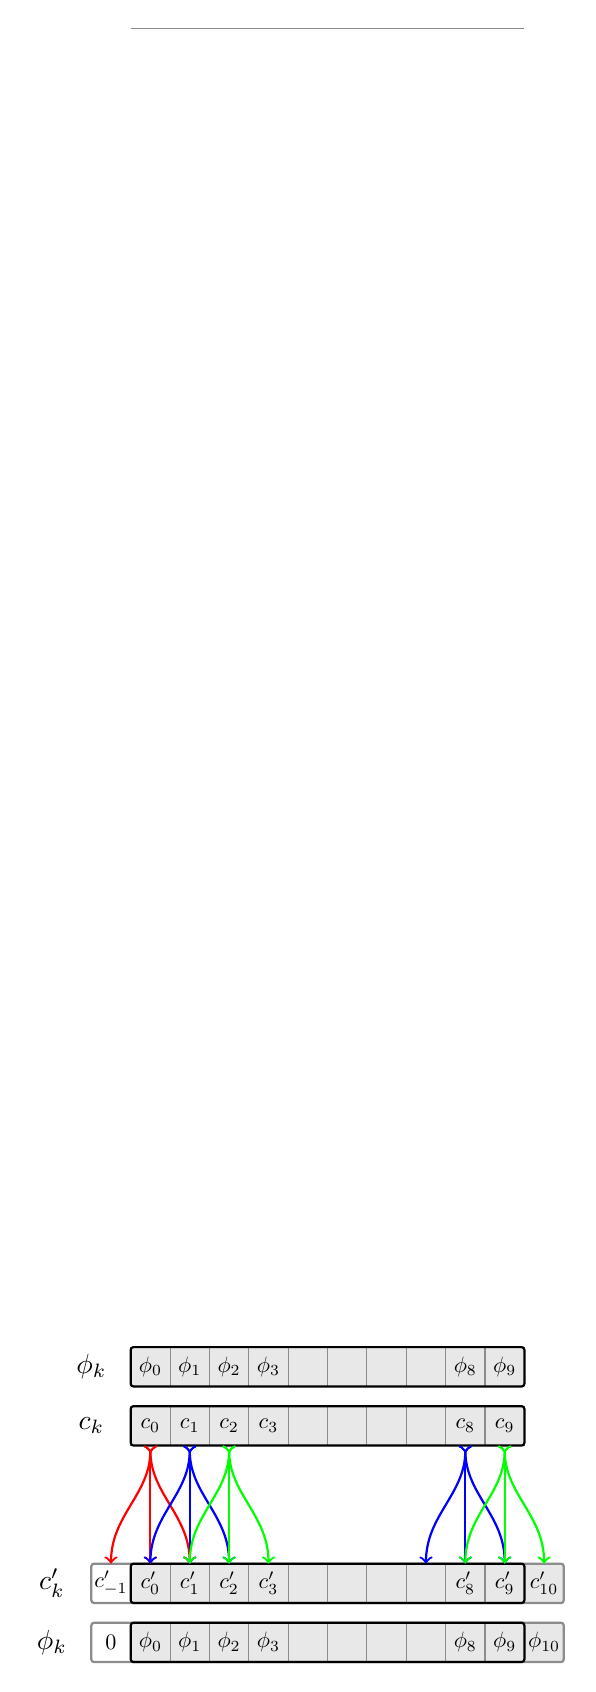
\begin{tikzpicture}
  \coordinate (co0) at (0.25, 2.0);
  \coordinate (co1) at (0.75, 2.0);
  \coordinate (co2) at (1.25, 2.0);
  \coordinate (co3) at (1.75, 2.0);
  \coordinate (co8) at (4.25, 2.0);
  \coordinate (co9) at (4.75, 2.0);

  \coordinate (cpm1) at (-0.25, 0.5);
  \coordinate (cp0) at (0.25, 0.5);
  \coordinate (cp1) at (0.75, 0.5);
  \coordinate (cp2) at (1.25, 0.5);
  \coordinate (cp3) at (1.75, 0.5);
  \coordinate (cp7) at (3.75, 0.5);
  \coordinate (cp8) at (4.25, 0.5);
  \coordinate (cp9) at (4.75, 0.5);
  \coordinate (cp10) at (5.25, 0.5);

  % upper
  \fill[gray!20, rounded corners=1] (0.0,2.0) rectangle (5.0,2.5);
  \draw[step=5mm, gray] (0,2.0) grid (5,2.5);
  \draw[black, thick, rounded corners=1] (0.0,2.0) rectangle (5.0,2.5);

  \fill[gray!20, rounded corners=1] (0.0,2.75) rectangle (5.0,3.25);
  \draw[step=5mm, ystep=20cm, gray] (0.0,2.75) grid (5.0,3.25);
  \draw[black, thick, rounded corners=1] (0.0,2.75) rectangle (5.0,3.25);

  % lower
  \fill[gray!20, rounded corners=1] (0.0,-0.75) rectangle (5.5,-0.25);
  \draw[step=5mm, ystep=20cm, gray] (0.0,-0.75) grid (5.0,-0.25);
  \draw[gray, thick, rounded corners=1] (-0.5,-0.75) rectangle (5.5,-0.25);
  \draw[black, thick, rounded corners=1] (0.0,-0.75) rectangle (5.0,-0.25);

  \fill[gray!20, rounded corners=1] (0.0,0.0) rectangle (5.5,0.5);
  \draw[step=5mm, gray] (0.0,0.0) grid (5.0,0.5);
  \draw[gray, thick, rounded corners=1] (-0.5,0.0) rectangle (5.5,0.5);
  \draw[black, thick, rounded corners=1] (0.0,0.0) rectangle (5.0,0.5);

  \draw[>->, thick, color=red] (co0) to[out=270,in=90] (cpm1);
  \draw[>->, thick, color=red] (co0) to[out=270,in=90] (cp0);
  \draw[>->, thick, color=red] (co0) to[out=270,in=90] (cp1);

  \draw[>->, thick, color=blue] (co1) to[out=270,in=90] (cp0);
  \draw[>->, thick, color=blue] (co1) to[out=270,in=90] (cp1);
  \draw[>->, thick, color=blue] (co1) to[out=270,in=90] (cp2);

  \draw[>->, thick, color=green] (co2) to[out=270,in=90] (cp1);
  \draw[>->, thick, color=green] (co2) to[out=270,in=90] (cp2);
  \draw[>->, thick, color=green] (co2) to[out=270,in=90] (cp3);

  \draw[>->, thick, color=blue] (co8) to[out=270,in=90] (cp7);
  \draw[>->, thick, color=blue] (co8) to[out=270,in=90] (cp8);
  \draw[>->, thick, color=blue] (co8) to[out=270,in=90] (cp9);

  \draw[>->, thick, color=green] (co9) to[out=270,in=90] (cp8);
  \draw[>->, thick, color=green] (co9) to[out=270,in=90] (cp9);
  \draw[>->, thick, color=green] (co9) to[out=270,in=90] (cp10);

  \node[scale=0.8] at (0.25,2.25) [black] {$c_0$};
  \node[scale=0.8] at (0.75,2.25) [black] {$c_1$};
  \node[scale=0.8] at (1.25,2.25) [black] {$c_2$};
  \node[scale=0.8] at (1.75,2.25) [black] {$c_3$};
  \node[scale=0.8] at (4.25,2.25) [black] {$c_8$};
  \node[scale=0.8] at (4.75,2.25) [black] {$c_9$};

  \node[scale=0.8] at (-0.25,0.25) [black] {$c^\prime_{-1}$};
  \node[scale=0.8] at (0.25,0.25) [black] {$c^\prime_0$};
  \node[scale=0.8] at (0.75,0.25) [black] {$c^\prime_1$};
  \node[scale=0.8] at (1.25,0.25) [black] {$c^\prime_2$};
  \node[scale=0.8] at (1.75,0.25) [black] {$c^\prime_3$};
  \node[scale=0.8] at (4.25,0.25) [black] {$c^\prime_8$};
  \node[scale=0.8] at (4.75,0.25) [black] {$c^\prime_9$};
  \node[scale=0.8] at (5.25,0.25) [black] {$c^\prime_{10}$};

  \node[scale=0.8] at (0.25,3.0) [black] {$\phi_0$};
  \node[scale=0.8] at (0.75,3.0) [black] {$\phi_1$};
  \node[scale=0.8] at (1.25,3.0) [black] {$\phi_2$};
  \node[scale=0.8] at (1.75,3.0) [black] {$\phi_3$};
  \node[scale=0.8] at (4.25,3.0) [black] {$\phi_8$};
  \node[scale=0.8] at (4.75,3.0) [black] {$\phi_9$};

  \node[scale=0.8] at (-0.25,-0.5) [black] {$0$};
  \node[scale=0.8] at (0.25,-0.5) [black] {$\phi_0$};
  \node[scale=0.8] at (0.75,-0.5) [black] {$\phi_1$};
  \node[scale=0.8] at (1.25,-0.5) [black] {$\phi_2$};
  \node[scale=0.8] at (1.75,-0.5) [black] {$\phi_3$};
  \node[scale=0.8] at (4.25,-0.5) [black] {$\phi_8$};
  \node[scale=0.8] at (4.75,-0.5) [black] {$\phi_9$};
  \node[scale=0.8] at (5.25,-0.5) [black] {$\phi_{10}$};

  \node at (-0.5,3.0) [black] {$\phi_{k}$};
  \node at (-1.0,-0.5) [black] {$\phi_{k}$};
  \node at (-0.5,2.25) [black] {$c_{k}$};
  \node at (-1.0,0.25) [black] {$c^\prime_{k}$};
\end{tikzpicture}

  \caption[Scatter-type stencil in 1D] {The scatter-type stencil application for
           computing the gradient $y\Phi$. The upper two arrays show the initial linear
           combination $\Phi$ consisting of basis functions $\phi_k$ and coefficients $c_k$.
           The lower two arrays show the linear combination of $\diff{\Phi}{x}$ consisting
           of the same basis functions $\phi_k$ and new coefficients $c_k^\prime$.
           Each of the triple arrows represents the computation for a fixed $\vec{k} \in \mathfrak{K}$
           (formula \eqref{eq:grad_basis_function_DD}), not all computations are shown.
           We see that the basis shape $\overline{\mathfrak{K}}$ for the gradient
           has to be larger. And also that we write to several elements not part
           of the original basis shape $\mathfrak{K}$. We drop the coefficient
           $c_{-1}^\prime$ (because $\phi_{-1} \equiv 0$).
           The original basis shape $\mathfrak{K}$ is represented by the black rectangle
           and the actual basis shapes are shown shaded grey.}
  \label{fig:grad_phi_kl_scatter_stencil_1D}
\end{figure}

\begin{figure}
  \centering
  \begin{tikzpicture}[scale=1,every node/.style={minimum size=0.5cm},on grid]

  \begin{scope}[
      yshift=-100,
      every node/.append style={yslant=0.5, xslant=-1.3},
      yslant=0.5,
      xslant=-1.3
    ]
    \coordinate (c32) at (1.75, 1.25);
    \coordinate (co25) at (1.25, 2.75);
  \end{scope}

  \begin{scope}[
      yshift=-160,
      every node/.append style={yslant=0.5, xslant=-1.3},
      yslant=0.5,
      xslant=-1.3
    ]
    \coordinate (cp42) at (2.25, 1.25);
    \coordinate (cp32) at (1.75, 1.25);
    \coordinate (cp22) at (1.25, 1.25);
    \coordinate (cp33) at (1.75, 1.75);
    \coordinate (cp31) at (1.75, 0.75);

    \coordinate (cop15) at (0.75, 2.75);
    \coordinate (cop25) at (1.25, 2.75);
    \coordinate (cop35) at (1.75, 2.75);
    \coordinate (cop24) at (1.25, 2.25);
    \coordinate (cop26) at (1.25, 3.25);
  \end{scope}

  % lower plane
  \begin{scope}[
      yshift=-160,
      every node/.append style={yslant=0.5, xslant=-1.3},
      yslant=0.5,
      xslant=-1.3
    ]
    \draw[step=5mm, thin, gray] (-0.5,-0.5) grid (3.5,3.5);

    \fill[blue!60] (2,1) rectangle (2.5,1.5);
    \node at (cp42) [draw, color=blue] {};%{$c^\prime_{4,2}$};

    \fill[blue!60] (1.5,1) rectangle (2.0,1.5);
    \node at (cp32) [draw, color=blue] {};%{$c^\prime_{3,2}$};

    \fill[blue!60] (1,1) rectangle (1.5,1.5);
    \node at (cp22) [draw, color=blue] {};%{$c^\prime_{2,2}$};

    \fill[blue!60] (1.5,1.5) rectangle (2.0,2.0);
    \node at (cp33) [draw, color=blue] {};%{$c^\prime_{3,3}$};

    \fill[blue!60] (1.5,0.5) rectangle (2.0,1.0);
    \node at (cp31) [draw, color=blue] {};%{$c^\prime_{3,1}$};

    \fill[orange!60] (0.5,2.5) rectangle (1.0,3.0);
    \node at (cop15) [draw, color=orange] {};%{$c^\prime_{1,5}$};

    \fill[orange!60] (1.0,2.5) rectangle (1.5,3.0);
    \node at (cop25) [draw, color=orange] {};%{$c^\prime_{2,5}$};

    \fill[orange!60] (1.5,2.5) rectangle (2.0,3.0);
    \node at (cop35) [draw, color=orange] {};%{$c^\prime_{3,5}$};

    \fill[orange!60] (1.0,2.0) rectangle (1.5,2.5);
    \node at (cop24) [draw, color=orange] {};%{$c^\prime_{2,4}$};

    \fill[orange!60] (1.0,3.0) rectangle (1.5,3.5);
    \node at (cop26) [draw, color=orange] {};%{$c^\prime_{2,6}$};

    \draw[black,thick, rounded corners=1] (0,0) rectangle (3,3);
    \draw[gray,thick, rounded corners=1] (-0.5,-0.5) rectangle (3.5,3.5);
  \end{scope}

  % arrows
  \begin{scope}
    \draw[>->, thick] (c32) node[left,scale=1.3] {} to[out=270,in=90] (cp42);
    \draw[>->, thick] (c32) node[left,scale=1.3] {} to[out=270,in=90] (cp32);
    \draw[>->, thick] (c32) node[left,scale=1.3] {} to[out=270,in=90] (cp22);
    \draw[>->, thick] (c32) node[left,scale=1.3] {} to[out=270,in=90] (cp33);
    \draw[>->, thick] (c32) node[left,scale=1.3] {} to[out=270,in=90] (cp31);

    \draw[>->, thick] (co25) node[left,scale=1.3] {} to[out=270,in=90] (cop24);
    \draw[>->, thick] (co25) node[left,scale=1.3] {} to[out=270,in=90] (cop25);
    \draw[>->, thick] (co25) node[left,scale=1.3] {} to[out=270,in=90] (cop26);
    \draw[>->, thick] (co25) node[left,scale=1.3] {} to[out=270,in=90] (cop15);
    \draw[>->, thick] (co25) node[left,scale=1.3] {} to[out=270,in=90] (cop35);
  \end{scope}

  % upper plane
  \begin{scope}[
      yshift=-100,
      every node/.append style={yslant=0.5, xslant=-1.3},
      yslant=0.5,
      xslant=-1.3
    ]
    \fill[white,fill opacity=0.8] (0,0) rectangle (3,3);
    \draw[step=5mm, thin, gray] (0,0) grid (3,3);

    \fill[blue!60] (1.5,1) rectangle (2.0,1.5);
    \node at (c32) [draw, color=blue] {};%{$c_{3,2}$};

    \fill[orange!60] (1.0,2.5) rectangle (1.5,3.0);
    \node at (co25) [draw, color=orange] {};%{$c_{2,5}$};

    \draw[black,thick, rounded corners=1] (0,0) rectangle (3,3);
  \end{scope}

  \node at (-3.25cm,-1.5cm) [black] {$c_{k,l}$};
  \node at (-4cm,-5.5cm) [black] {$\vec{c}^\prime_{k,l}$};
\end{tikzpicture}

  \caption[Scatter-type stencil in 2D] {The scatter-type stencil application for
           computing the gradient $y\Phi$. The upper array (plane) shows the
           coefficients $c_{\vec{k}}$ of the initial linear combination $\Phi(\vec{x})$.
           The lower array (plane) shows the coefficients $\vec{c}^\prime_{\vec{k}}$ of the
           linear combination of $\nabla\Phi(\vec{x})$ where each square is not a single
           number but stands for a whole vector. Each arrow bundle represents the
           computation for a fixed $\vec{k} \in \mathfrak{K}$ (formula
           \eqref{eq:grad_basis_function_DD}), not all computations are shown.
           The original basis shape $\mathfrak{K}$ is given by the black rectangle.
           We then see that the basis shape $\overline{\mathfrak{K}}$ for the gradient
           is larger by one square on each side. (But we again drop all coefficients
           with negative index.)
           The orange stencil shows that we sometimes have to write to elements
           (coefficients) that are not part of the original basis shape. Therefore
           we need to extend the basis shape where the whole lower plane stands
           for $\overline{\mathfrak{K}}$.
}
  \label{fig:grad_phi_kl_scatter_stencil_2D}
\end{figure}

\begin{algorithm}
\caption{Compute the gradient $y \Phi$ by scatter-type stencil application}
\label{al:grad_phi_scatter_type}
\begin{algorithmic}
  \REQUIRE Scalar wavepacket $\Phi$ in $D$ space dimensions
  \REQUIRE Basis shape $\mathfrak{K}$ (including linearisation mapping $\mu_{\mathfrak{K}}$) of $\Phi$
  \REQUIRE Parameters $\Pi$ and coefficients $\{c_{\vec{k}}\}$ of $\Phi$

  \STATE // Extend the basis shape $\mathfrak{K}$
  \STATE $\overline{\mathfrak{K}} \assign \text{\bf{extend\_basis\_shape}}(\mathfrak{K})$

  \STATE // Storage space for the result
  \STATE $\mat{c}^\prime = \mat{0} \in \mathbb{C}^{D \times |\overline{\mathfrak{K}}|}$

  \STATE // Iterate over original basis shape
  \FOR{$\vec{k} \in \mathfrak{K}$}

    \STATE // Central node
    \STATE $\mat{c}^\prime[:,\mu_{\overline{\mathfrak{K}}}(\vec{k})] =
            \mat{c}^\prime[:,\mu_{\overline{\mathfrak{K}}}(\vec{k})] +
            c_{\vec{k}} \, \vec{p}$

    \STATE // Backward neighbours
    \FOR{$d = 0$ \TO $d = D-1$}
      \STATE $\vec{k}^\prime = \vec{k} - \vec{e}^d$
      \IF{$\vec{k}^\prime \in \overline{\mathfrak{K}}$}
        \STATE $\mat{c}^\prime[:,\mu_{\overline{\mathfrak{K}}}(\vec{k}^\prime)] =
                \mat{c}^\prime[:,\mu_{\overline{\mathfrak{K}}}(\vec{k}^\prime)] +
                \sqrt{\frac{\varepsilon^2}{2}} \sqrt{\vec{k}[d]} \, c_{\vec{k}} \, \conj{\mat{P}}[:,d]$
      \ENDIF
    \ENDFOR

    \STATE // Forward neighbours
    \FOR{$d = 0$ \TO $d = D-1$}
      \STATE $\vec{k}^\prime = \vec{k} + \vec{e}^d$
      \IF{$\vec{k}^\prime \in \overline{\mathfrak{K}}$}
        \STATE $\mat{c}^\prime[:,\mu_{\overline{\mathfrak{K}}}(\vec{k}^\prime)] =
                \mat{c}^\prime[:,\mu_{\overline{\mathfrak{K}}}(\vec{k}^\prime)] +
                \sqrt{\frac{\varepsilon^2}{2}} \sqrt{\vec{k}[d]+1} \, c_{\vec{k}} \, \mat{P}[:,d]$
      \ENDIF
    \ENDFOR

  \ENDFOR
  \RETURN $\overline{\mathfrak{K}}$ and $\mat{c}^\prime$
\end{algorithmic}
\end{algorithm}


\subsection{An example}


As an example we take a wavepacket $\Ket{\Psi}$ in two space dimensions with the
following parameter set $\Pi = \{\vec{0}, \vec{0}, \id, i \id \}$ and $\varepsilon = 0.6$.
The coefficients are set to the values printed in the next table.

\begin{center}
\begin{tabular}{l r}
$\vec{k}$ & $c_{\vec{k}}$ \\
\hline
$(0,0)$ & $0.5$ \\
$(0,1)$ & $0.5$ \\
$(1,1)$ & $0.5$ \\
$(2,1)$ & $0.5$
\end{tabular}
\end{center}

A plot of the wavepacket evaluated on a small region of position space is shown
in figure \ref{fig:wavepacket_original}.

\begin{figure}
  \centering
  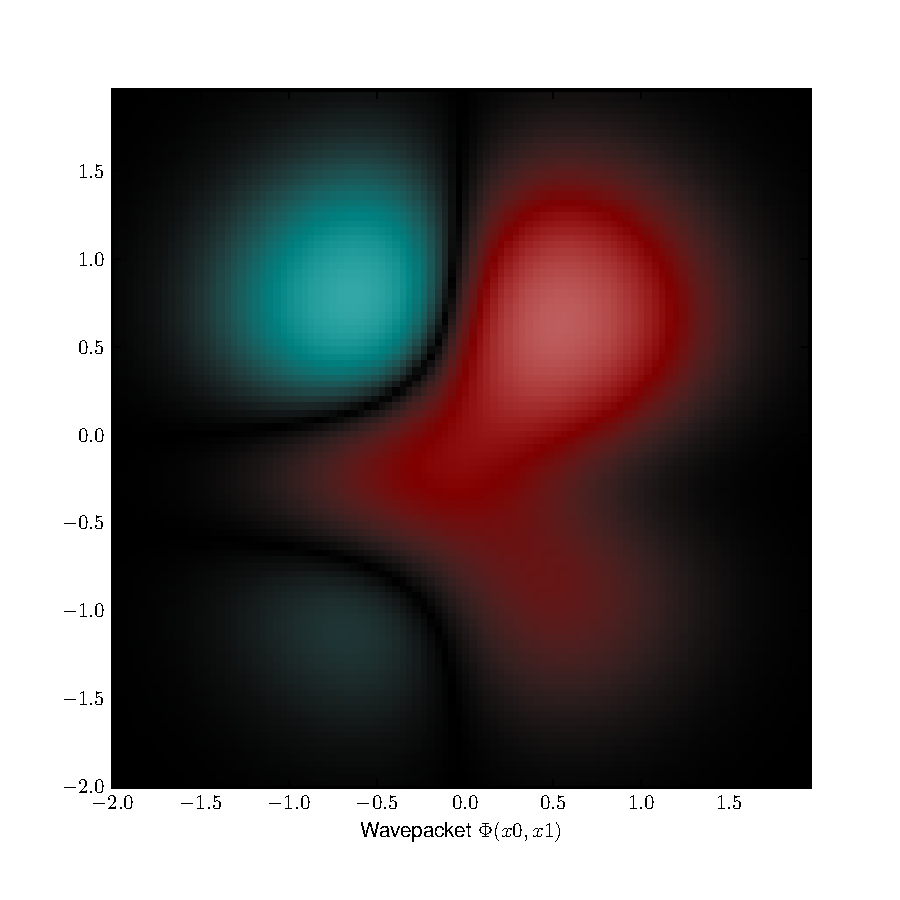
\includegraphics[scale=0.3]{./fig/wavepacket_original.pdf}
  \caption[Wavepacket of the gradient example]{The wavepacket $\Ket{\Psi}$.}
  \label{fig:wavepacket_original}
\end{figure}

Next we compute the gradient $-i \varepsilon \nabla \Psi$ by one of the above
methods. For the new coefficients $\vec{c}_{\vec{k}}$ we get the values (only
non-zero ones) shown in the next table. The two components of the gradient
are plotted in figure \ref{fig:wavepacket_gradient}.

\begin{center}
\begin{tabular}{l r r}
$\vec{k}$ & $x_0$ component of $\vec{c}_{\vec{k}}$ &  $x_1$ component of $\vec{c}_{\vec{k}}$ \\
\hline
$(0,0)$ &$0$                            & $- 0.21213203 \mathbf{\imath}$ \\
$(0,1)$ &$- 0.21213203 \mathbf{\imath}$ & $0.21213203 \mathbf{\imath}$ \\
$(1,0)$ &$0.21213203 \mathbf{\imath}$   & $- 0.21213203 \mathbf{\imath}$ \\
$(1,1)$ &$- 0.08786797 \mathbf{\imath}$ & $0$  \\
$(2,0)$ &$0$                            & $- 0.21213203 \mathbf{\imath}$ \\
$(2,1)$ &$0.3 \mathbf{\imath}$          & $0$  \\
$(3,1)$ &$0.36742346 \mathbf{\imath}$   & $0$  \\
$(0,2)$ &$0$                            & $0.3 \mathbf{\imath}$ \\
$(1,2)$ &$0$                            & $0.3 \mathbf{\imath}$ \\
$(2,2)$ &$0$                            & $0.3 \mathbf{\imath}$ \\
\end{tabular}

\end{center}\begin{figure}
  \centering
  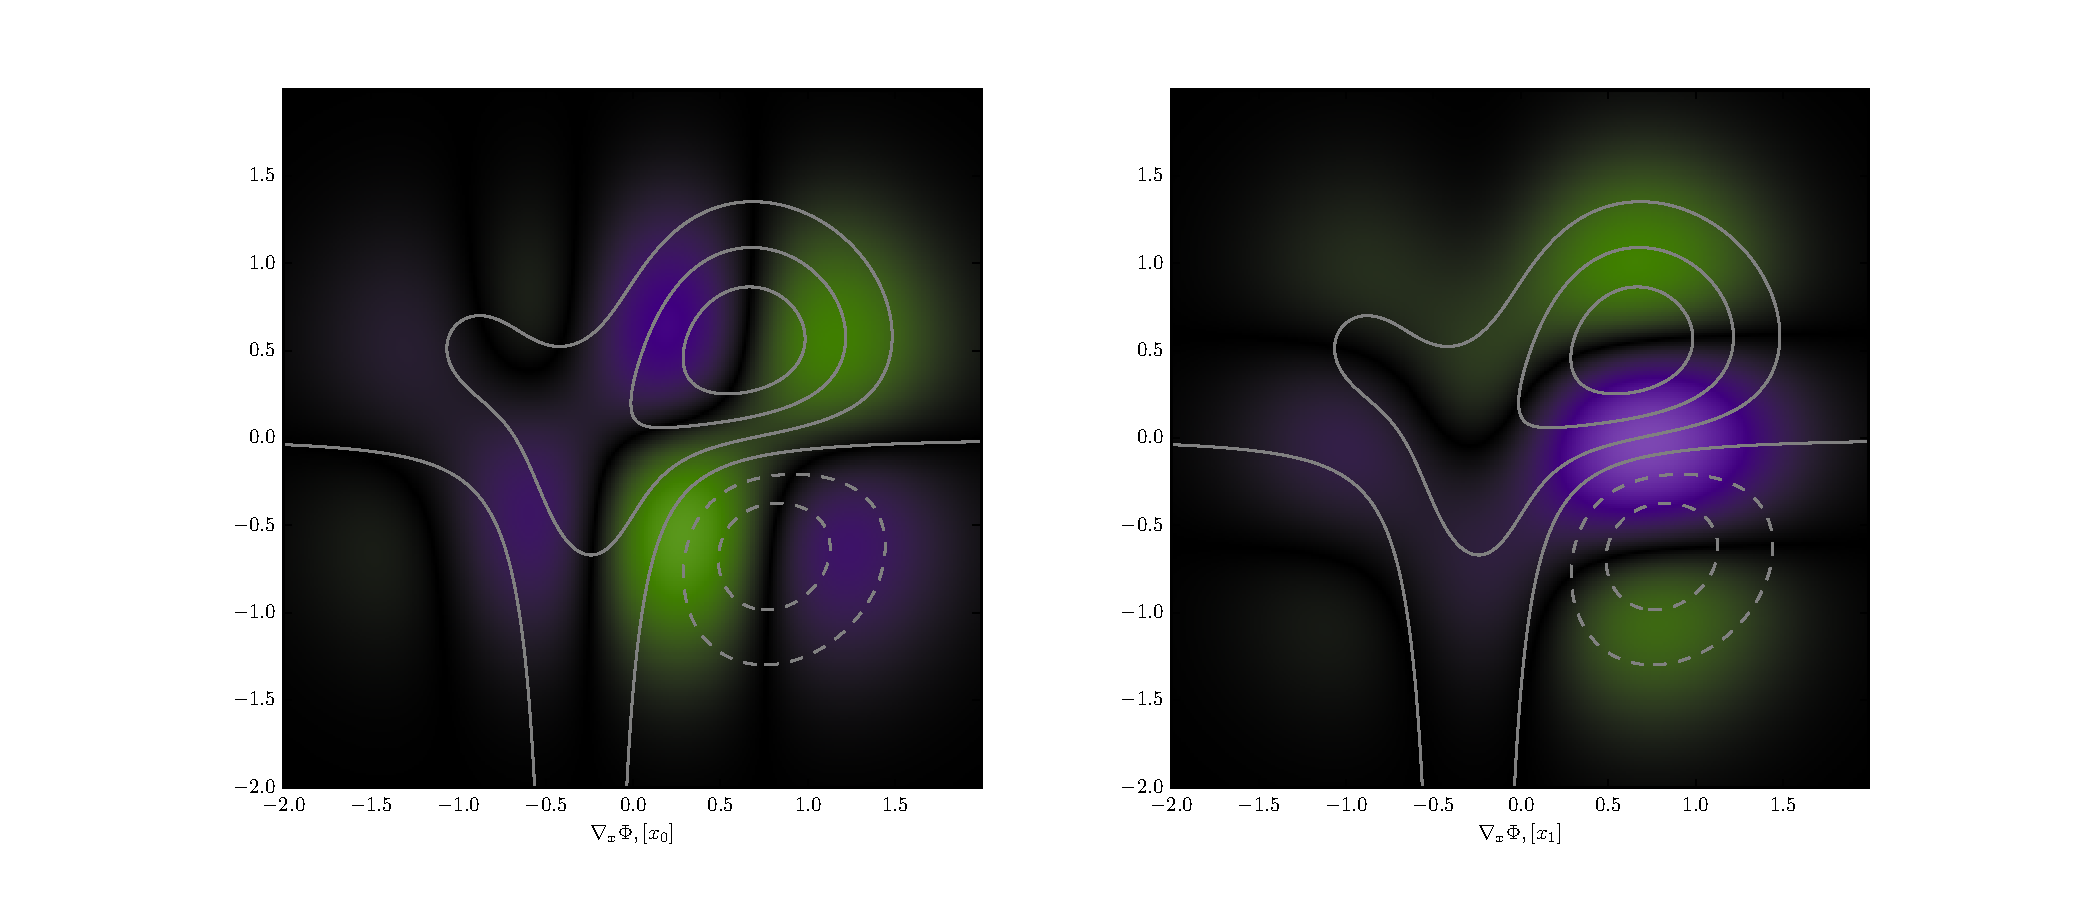
\includegraphics[scale=0.32]{./fig/wavepacket_gradient.pdf}
  \caption[Plots of the gradient example]
          {The $x_0$ (left) and $x_1$ (right) components of the gradient
           $-i \varepsilon \nabla \Psi$. The wavepacket $\Psi$ is indicated
           by some contour levels just for reference.}
  \label{fig:wavepacket_gradient}
\end{figure}

Finally, figure \ref{fig:wavepacket_coefficients} shows again the coefficients
of both, the original wavepacket and the two components of its gradient.

\begin{figure}
  \centering
  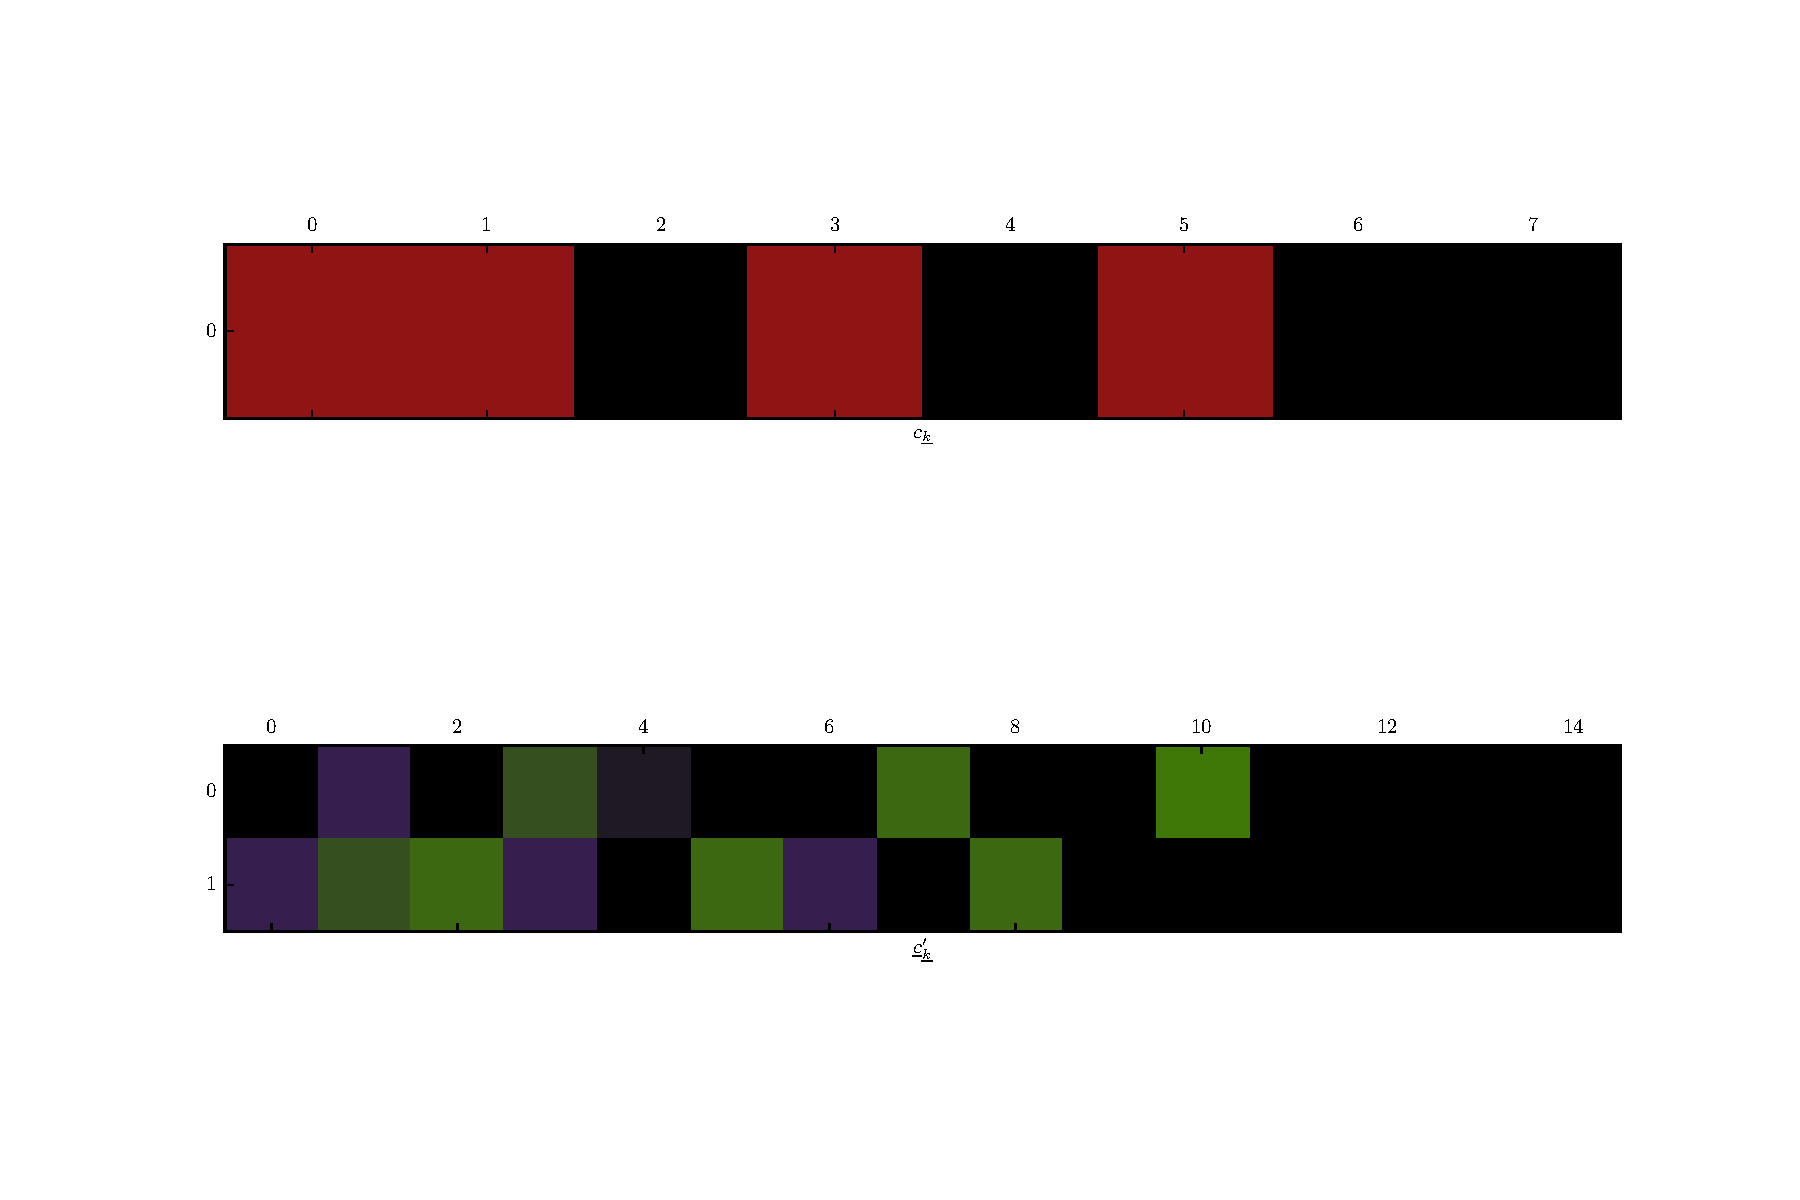
\includegraphics[width=0.8\linewidth]{./fig/wavepacket_coefficients.pdf}
  \caption[Coefficients of the gradient example]
         {Coefficients $c_{\vec{k}}$ of $\Psi$ (top) and $\vec{c}_{\vec{k}}$ of
          $-i \varepsilon \nabla \Psi$ (bottom). Notice also the different basis
          sizes $|\mathfrak{K}|$ of 8 and 15.}
  \label{fig:wavepacket_coefficients}
\end{figure}

\chapter{Observables and Inner Products}
\label{ch:observables}

In this chapter we develop the machinery necessary to get information out of the
wavepackets whose time-evolution we will simulate. An essential part is the computation
of several types of brakets. This will be done numerically by a special, high-order
quadrature rule.


\section{Observables in general}


To compute any observable $O$ we have to form the full braket:

\begin{equation}
  O = \Braket{\Psi | \hat{O} | \Psi}
\end{equation}

which boils down to a multi-dimensional integral. We look at the most general
case and seek to compute:

\begin{equation}
  \Braket{\Psi^\prime | \mathcal{F} | \Psi}
\end{equation}

where the operator $\mathcal{F}$ is a $N \times N$ matrix of scalar functions
$\mathcal{F}_{r,c}(\vec{x})$. The wavepackets $\Psi$ and $\Psi^\prime$ are
assumed to be of inhomogeneous type and can have different parameter sets
$\Pi$ and $\Pi^\prime$. The ansatz is:

\begin{align*}
  \Braket{\Psi^\prime | \mathcal{F} | \Psi} & =
  \Braket{
    \begin{pmatrix}
      \Phi_0^\prime \\ \vdots \\ \Phi_{N-1}^\prime
    \end{pmatrix}
    |
    \begin{pmatrix}
      {}     & \vdots            & {} \\
      \cdots & \mathcal{F}_{r,c} & \cdots \\
      {}     & \vdots            & {}
    \end{pmatrix}
    |
    \begin{pmatrix}
      \Phi_0 \\ \vdots \\ \Phi_{N-1}
    \end{pmatrix}
  } \\
  & =
  \sum_{r=0}^{N-1} \sum_{c=0}^{N-1}
  \Braket{\Phi_r^\prime | \mathcal{F}_{r,c} | \Phi_c} \,.
\end{align*}

We continue by using the definition \eqref{eq:scalar_wavepacket} for the
individual components and resolve:

\begin{align*}
  \Braket{\Phi^\prime_r | \mathcal{F}_{r,c} | \Phi_c} & =
  \Braket{\sum_{\vec{k}\in\mathfrak{K}^\prime_r} \phi^\prime_{\vec{k}}
          | \mathcal{F}_{r,c} |
          \sum_{\vec{l}\in\mathfrak{K}_c} \phi_{\vec{l}}} \\
  & =
  \sum_{\vec{k}\in\mathfrak{K}^\prime_r}
  \sum_{\vec{l}\in\mathfrak{K}_c}
  \Braket{\phi^\prime_{\vec{k}} | \mathcal{F}_{r,c} | \phi_{\vec{l}}}
\end{align*}

where we left out the global phase as well as the coefficients. The last
braket consists of basis functions only and we know that:

\begin{equation*}
  \Braket{\phi^\prime_{\vec{k}} | \mathcal{F}_{r,c} | \phi_{\vec{l}}}
  =
  \idotsint \conj{\phi^\prime_{\vec{k}}(\vec{x})} \mathcal{F}_{r,c}(\vec{x}) \phi_{\vec{l}}(\vec{x}) \mathrm{d}\vec{x} \,.
\end{equation*}

Hence we make a longer detour and examine the computation of any
inner-product like this one before we return to observables.


\section{Inner products}


\subsection{Integrals over basis functions}


In the following we want to compute inner products of the form
$\Braket{\phi_k[\Pi_k]|\phi_l[\Pi_l]}$ with just an identity
in place of $\mathcal{F}_{r,c}$ from above. We abuse the notation
here. The indices $k$ and $l$ are not multi-indices and do not index
the $\phi$ in the corresponding basis set. They are solely used to
discriminate between the bra and the ket, to make clear which
function $\phi$ and parameter set $\Pi$ we speak of. There is no useful
closed form solution to this integral and we have to compute it
numerically by using quadrature. For the derivation of the quadrature
formulae we work with the ground states only and hence $\phi_k = \phi^\prime_{\vec{0}}$
and $\phi_l = \phi_{\vec{0}}$.


\subsection{Quadrature rules}


To compute the integral shown in the last section we use a Gauss-Hermite
quadrature rule of very high order. The properties of this quadrature rule
make it well-suited for our purpose. The quadrature rule $\rho$ consists of
nodes $\gamma$ and weights $\omega$. In the case of Gauss-Hermite quadrature
these values are built to integrate $f(x)$ in:

\begin{equation} \label{eq:gh_integral}
  \int_{\mathbb{R}} e^{-x^2} f(x) \mathrm{d}x \approx \sum_{i=0}^{R-1} \omega_i f(\gamma_i) \,.
\end{equation}

For a quadrature of order $R$ the nodes $\{\gamma_i\}_{i=0}^{R-1}$ are then
given as the roots of the Hermite polynomial $H_R(x)$:

\begin{equation*}
  H_R(x) = (-1)^R e^{x^2} \frac{d^R}{dx^R} e^{-x^2} \,.
\end{equation*}

Of course we do not compute the nodes by finding the roots of these polynomials
as this is inherently unstable. The quadrature weights are then given by:

\begin{equation*}
  \omega_i = \frac{2^{R-1} R! \sqrt{\pi}} {R^2 H_{R-1}^2(\gamma_i)} \,.
\end{equation*}

Since our integrals are not of the form \eqref{eq:gh_integral}
but instead we have:

\begin{equation}
  \int_{\mathbb{R}} g(x) \mathrm{d}x
\end{equation}

where the $\exp(-x^2)$ is built into the function $g(x)$ such that
$g(x) = \exp(-x^2) f(x)$, we have to alter the ansatz. We can not divide
by $\exp(-x^2)$ without getting major numerical instabilities. But we can
modify our quadrature weights to take that factor into account. We define
new quadrature weights $\omega_i^\prime$ as:

\begin{equation*}
  \omega_i^\prime \assign \frac{1}{R \, h_R^2(\gamma_i)}
\end{equation*}

where $h_R$ are the Hermite functions defined as:

\begin{equation*}
  h_R(x) \assign \frac{1}{\sqrt{2^R R! \sqrt{\pi}}} e^{-x^2/2} H_R(x) \,.
\end{equation*}

We can evaluate the Hermite function for any point $x$ by a stable,
recursive scheme. Finally the quadrature rule $\rho$ in use is
given by:

\begin{equation}
  \rho \assign \left\{\left(\gamma_i, \omega_i^\prime\right)\right\}_{i=0}^{R-1}
\end{equation}

for one space dimension. In higher dimensions we build a quadrature
rule $\rho$ by computing the full tensor product of $D$ one-dimensional
quadrature rules $\rho_d$:

\begin{equation}
  \rho \assign \bigotimes_{d=0}^{D-1} \rho_d \,.
\end{equation}

Using the rules $\rho_d$, each of order $R_d$, we get the $D$-dimensional
rule then denoted by:

\begin{equation}
  \rho \assign \left\{ \left( \vec{\gamma}_i, \omega_i \right) \right\}_{i=0}^{R-1}
\end{equation}

with a total number $R = \prod_{d=0}^{D-1} R_d$ of quadrature nodes. The quadrature
nodes $\vec{\gamma}_{\vec{j}} \in \mathbb{R}^D$ are constructed as:

\begin{equation*}
  \vec{\gamma}_{\vec{j}}
  \assign
  \begin{pmatrix}
    \gamma^0_{\vec{j}_0} \\
    \vdots \\
    \gamma^{D-1}_{\vec{j}_{D-1}}
  \end{pmatrix}
\end{equation*}

with $\vec{j} \in [0,R_0-1] \times \cdots \times [0,R_{D-1}-1]$ a multi-index.
Each of the $\gamma^d$ belongs to the one-dimensional rule $\rho_d$. For the
weights $\omega_i$ of $\rho$ we have:

\begin{equation*}
  \omega_{\vec{j}} \assign \prod_{d=0}^{D-1} \omega^d_{\vec{j}_d}
\end{equation*}

and again $\omega^d$ is part of $\rho_d$. Figure \ref{fig:tensor_product_qr}
shows a typical two-dimensional quadrature rule.

\begin{figure}
  \centering
  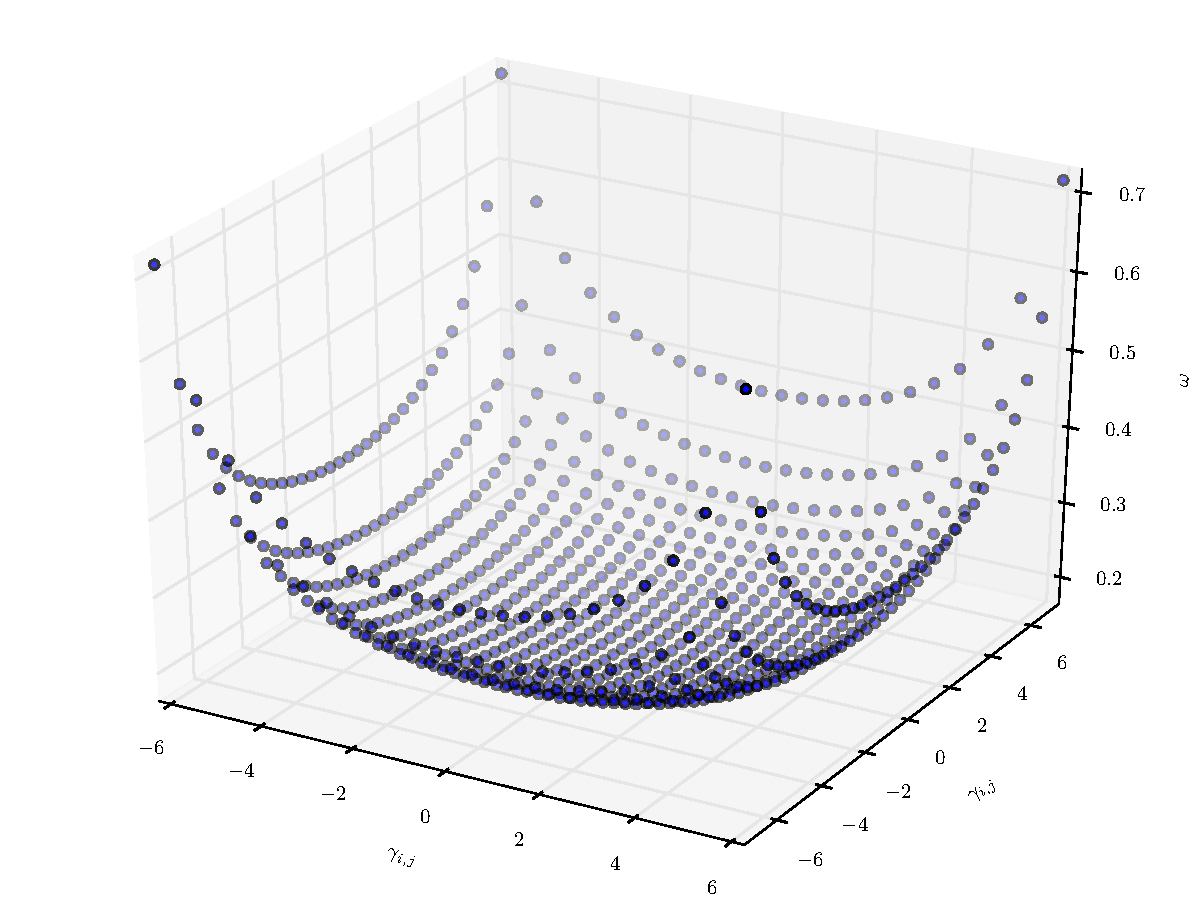
\includegraphics[width=0.8\linewidth]{./fig/tensor_qr.pdf}
  \caption[A two-dimensional quadrature rule]{
    Plot of the nodes $\vec{\gamma}_i$ and weights $\omega_i$ of
    a two-dimensional quadrature rule $\rho$. The rule is build
    from two one-dimensional rules of order $24$ and $32$.
  }
  \label{fig:tensor_product_qr}
\end{figure}


\subsection{Adapting the quadrature}


Since the basis functions are parametrised we have to adapt the quadrature rule
$\{\vec{\gamma_i}, \omega_i\}_i$ to fit best the given situation depending on the
sets $\Pi_k$ and $\Pi_l$. If both functions in the bra and the ket are members of
the same family with $\Pi_k \equiv \Pi_l$ the process is much easier and we will
do this case first. But we will need also the more general case where $\Pi_k \neq \Pi_l$
later. The purpose of this subsection is to find a transformation rule for the quadrature
nodes $\vec{\gamma_i}$ to suit the wavepacket's basis best. The final rule will
be an affine transformation like:

\begin{equation} \label{eq:transformed_qr_nodes}
  \vec{\gamma_i}^\prime = \vec{v} + \mat{A} \vec{\gamma_i}
\end{equation}

where the quadrature node $\vec{\gamma_i} \in \mathbb{R}^D$, the offset vector
$\vec{v} \in \mathbb{R}^D$ and the transformation matrix $\mat{A} \in \mathbb{R}^{D \times D}$.


\subsection{The homogeneous case}


We first threat the homogeneous case of the overlap integral. This case is
much easier as we assume that we have the same wavepacket in the bra as well
as in the ket. Hence the inner-product simplifies to $\Braket{\phi|\phi}$
and we have the same set $\Pi$ of Hagedorn Parameters. This makes combining
the two exponential terms from the definition \eqref{eq:phi0_Dd} into a single one
of the same form much easier.

We concentrate on the exponential parts which dominate the overall shape of the
basis functions and we are interested in the quadratic term only. Essentially we
only need to know where the peak of the Gaussian is and how big the spread is.

\begin{align*}
  \Braket{\phi|\phi} = & \\
  \exp\Bigg( &
      \conj{\frac{i}{2\varepsilon^2} \dotp{\ofs{\vec{x}-\vec{q}}}{\mat{P} \mat{Q}\inv \ofs{\vec{x}-\vec{q}}}
      + \frac{i}{\varepsilon^2} \dotp{\vec{p}}{\ofs{\vec{x}-\vec{q}}}}
      \\
    & + \frac{i}{2\varepsilon^2} \dotp{\ofs{\vec{x}-\vec{q}}}{\mat{P} \mat{Q}\inv \ofs{\vec{x}-\vec{q}}}
      + \frac{i}{\varepsilon^2} \dotp{\vec{p}}{\ofs{\vec{x}-\vec{q}}}
  \Bigg) \\
  = \exp\Bigg( &
      \frac{-i}{2\varepsilon^2} \conj{\dotp{\ofs{\vec{x}-\vec{q}}}{\mat{P} \mat{Q}\inv \ofs{\vec{x}-\vec{q}}}}
      + \frac{-i}{\varepsilon^2} \conj{\dotp{\vec{p}}{\ofs{\vec{x}-\vec{q}}}}
      \\
    & + \frac{i}{2\varepsilon^2} \dotp{\ofs{\vec{x}-\vec{q}}}{\mat{P} \mat{Q}\inv \ofs{\vec{x}-\vec{q}}}
      + \frac{i}{\varepsilon^2} \dotp{\vec{p}}{\ofs{\vec{x}-\vec{q}}}
  \Bigg) \\
  = \exp\Bigg( &
      \frac{-i}{2\varepsilon^2} \dotp{\mat{P} \mat{Q}\inv \ofs{\vec{x}-\vec{q}}}{\ofs{\vec{x}-\vec{q}}}
      + \frac{-i}{\varepsilon^2} \dotp{\ofs{\vec{x}-\vec{q}}}{\vec{p}}
      \\
    & + \frac{i}{2\varepsilon^2} \dotp{\ofs{\vec{x}-\vec{q}}}{\mat{P} \mat{Q}\inv \ofs{\vec{x}-\vec{q}}}
      + \frac{i}{\varepsilon^2} \dotp{\vec{p}}{\ofs{\vec{x}-\vec{q}}}
  \Bigg)
\end{align*}

For the sake of readability we define the matrix:

\begin{equation*}
  \mat{\Gamma} \assign \mat{P} \mat{Q}\inv
\end{equation*}

and continue. From now on we drop the exponential and work on the exponent only.
(The equal signs have to be understood within this laziness.)

\begin{align*}
  & =
    \frac{i}{2\varepsilon^2} \dotp{\ofs{\vec{x}-\vec{q}}}{\mat{\Gamma} \ofs{\vec{x}-\vec{q}}}
  - \frac{i}{2\varepsilon^2} \dotp{\mat{\Gamma} \ofs{\vec{x}-\vec{q}}}{\ofs{\vec{x}-\vec{q}}}
  + \frac{i}{\varepsilon^2} \dotp{\vec{p}}{\ofs{\vec{x}-\vec{q}}}
  - \frac{i}{\varepsilon^2} \dotp{\ofs{\vec{x}-\vec{q}}}{\vec{p}} \\
  & =
    \frac{i}{2\varepsilon^2} \Bigl( \dotp{\ofs{\vec{x}-\vec{q}}}{\mat{\Gamma} \ofs{\vec{x}-\vec{q}}} - \dotp{\mat{\Gamma} \ofs{\vec{x}-\vec{q}}}{\ofs{\vec{x}-\vec{q}}} \Bigr)
  + \frac{i}{\varepsilon^2} \Bigl( \dotp{\vec{p}}{\ofs{\vec{x}-\vec{q}}} - \dotp{\ofs{\vec{x}-\vec{q}}}{\vec{p}} \Bigr)
\end{align*}

The linear terms vanish as the inner-product is symmetric for entirely real arguments.
We then rearrange and combine the brakets:

\begin{align*}
  & =
  \frac{i}{2\varepsilon^2} \Bigl( \dotp{\ofs{\vec{x}-\vec{q}}}{\mat{\Gamma} \ofs{\vec{x}-\vec{q}}} - \dotp{\ofs{\vec{x}-\vec{q}}}{\mat{\Gamma}\H \ofs{\vec{x}-\vec{q}}} \Bigr) \\
  & =
  \frac{i}{2\varepsilon^2} \dotp{\ofs{\vec{x}-\vec{q}}}{\left(\mat{\Gamma} - \mat{\Gamma}\H\right) \ofs{\vec{x}-\vec{q}}} \,.
\end{align*}

Now we are almost done. The term on the last line is of the same form as the
quadratic one in the definition of $\Ket{\phi}$. Hence we succeeded in combining
the Gaussian exponential parts of two wavepackets into a single one.

The only thing left is to simplify the operator $\mat{\Gamma} - \mat{\Gamma}\H$ but this
is not difficult. Recalling the definition of $\mat{\Gamma}$ we get:

\begin{align*}
  \mat{\Gamma} - \mat{\Gamma}\H
  & = \mat{P} \mat{Q}\inv - \left(\mat{P} \mat{Q}\inv\right)\H \\
  & = \mat{P} \mat{Q}\inv - \mat{Q}\Hinv \mat{P}\H \\
  & = \mat{P} \mat{Q}\inv - \left(\mat{P} \mat{Q}\inv\right)\H \,.
\end{align*}

Remembering the second of the two compatibility conditions in \eqref{eq:PQcond_Dd} we get:

\begin{align*}
  \mat{Q}\H \mat{P} - \mat{P}\H \mat{Q} & = 2i \id \\
  \mat{Q}\Hinv \mat{Q}\H \mat{P} - \mat{Q}\Hinv \mat{P}\H \mat{Q} & = 2i \mat{Q}\Hinv \\
  \mat{P} \mat{Q}\inv - \mat{Q}\Hinv \mat{P}\H \mat{Q} \mat{Q}\inv & = 2i \mat{Q}\Hinv \mat{Q}\inv \\
  \mat{P} \mat{Q}\inv - \mat{Q}\Hinv \mat{P}\H & = 2i \mat{Q}\Hinv \mat{Q}\inv \\
  \mat{P} \mat{Q}\inv - \left(\mat{P} \mat{Q}\inv\right)\H & = 2i \left(\mat{Q} \mat{Q}\H\right)\inv
\end{align*}

where we used identities from \cite{P_matrix_book}. Hence:

\begin{equation*}
    \mat{\Gamma} - \mat{\Gamma}\H = 2i \left(\mat{Q} \mat{Q}\H\right)\inv \,.
\end{equation*}

We want the combined wavepacket to look like the following (which is motivated
by the reason that this exactly yields a Gaussian with shift $\vec{q_0}$ and spread $\mat{Q_0}$):

\begin{equation} \label{eq:desired_form}
  \exp{\left( -\frac{1}{\varepsilon^2} \dotp{\ofs{\vec{x}-\vec{q_0}}}{ \mat{Q_0} \ofs{\vec{x}-\vec{q_0}}} + \text{optional junk} \right)}
\end{equation}

where $\vec{q_0} \in \mathbb{R}^D$ and $\mat{Q_0} \in \mathbb{C}^{D \times D}$
are the final parameters to determine.

From above we have:

\begin{align*}
  & \exp\ofs{\frac{i}{2\varepsilon^2} \dotp{\ofs{\vec{x}-\vec{q}}}{\left(\mat{\Gamma} - \mat{\Gamma}\H\right) \ofs{\vec{x}-\vec{q}}}} \\
  & = \exp\ofs{\frac{i}{2\varepsilon^2} \dotp{\ofs{\vec{x}-\vec{q}}}{2i \left(\mat{Q} \mat{Q}\H\right)\inv \ofs{\vec{x}-\vec{q}}}} \\
  & = \exp\ofs{-\frac{1}{\varepsilon^2} \dotp{\ofs{\vec{x}-\vec{q}}}{\left(\mat{Q} \mat{Q}\H\right)\inv \ofs{\vec{x}-\vec{q}}}} \,.
\end{align*}

Therefore we immediately see that we have to set:

\begin{equation} \label{eq:quad_mix_Dd_homog_q0}
\boxed{
  \vec{q_0} = \vec{q}
}
\end{equation}

and:

\begin{equation} \label{eq:quad_mix_Dd_homog_Q0}
\boxed{
  \mat{Q_0} = \ofs{\mat{Q} \mat{Q}\H}\inv
}
\end{equation}

Notice that in the limit of $D \rightarrow 1$ we retrieve the scalar case
presented in \cite{B_bachelor_thesis} where $q_0 \in \mathbb{R}$ and
$Q_0 \in \mathbb{C}$ and:

\begin{align*}
  q_0 & = q \\
  Q_0 & = \ofs{Q \conj{Q}}\inv = \frac{1}{|Q|^2} \,.
\end{align*}


\subsection{The parameter $\mat{Q_S}$}


For the transformation of the quadrature rule $\{\vec{\gamma_i}, \omega_i\}_i$
the values $\mat{Q_0}$ and $\mat{q_0}$ are not enough. We need a parameter
denoted by $\mat{Q_S}$ which is in the one-dimensional case given by:

\begin{equation*}
  Q_S \assign \frac{1}{\sqrt{Q_0}} \,.
\end{equation*}

Therefore our next goal is to find a relation which holds in the $D$-dimensional
case too. We propose in analogy the following formula:

\begin{equation} \label{eq:mixing_Qs}
\boxed{
  \mat{Q_S} \assign \ofs{\sqrt{\mat{Q_0}}}\inv
}
\end{equation}

But we have to find a way to express the root of a matrix in a suitable way. There
is a way to compute almost any scalar function $f\ofs{x}$ for a matrix argument
$\mat{X}$. The trick goes by the similarity transform of $\mat{X}$ and then
computing $f$ on the eigenvalues $\lambda_i$ of $\mat{X}$. But this method relies
on $\mat{X}$ being diagonalisable and $f$ being defined on the whole spectrum of
$\mat{X}$. We will now take a longer but probably cleaner way which in the end
turns out to be not that different.

We are in the homogeneous case and thus $\mat{Q_0} = \ofs{\mat{Q} \mat{Q}\H}\inv$.
Refining the above expression step by step we get:

\begin{align*}
  \mat{Q_S} & \assign \ofs{\sqrt{\mat{Q_0}}}\inv \\
            & = \ofs{\sqrt{\ofs{\mat{Q} \mat{Q}\H}\inv}}\inv \\
            & = \ofs{\sqrt{\ofs{\mat{Q}\H}\inv \mat{Q}\inv}}\inv \\
            & = \ofs{\sqrt{\ofs{\mat{Q}\inv}\H \mat{Q}\inv}}\inv \,.
\end{align*}

If we now define $\mat{X} \assign \mat{Q}\inv$ we get:

\begin{equation}
  \mat{Q_S} \assign \ofs{\sqrt{\mat{X}\H \mat{X}}}\inv \,.
\end{equation}

For a complex square matrix $\mat{A}$ one can define the so called \emph{polar decomposition}
as follows:

\begin{equation*}
  \mat{A} \rassign \mat{U} \mat{P}
\end{equation*}

where $\mat{U}$ is unitary and $\mat{P}$ is a positive-semidefinite Hermitian matrix.
The two factors are given as:

\begin{align*}
  \mat{P} & \assign \sqrt{\mat{A}\H \mat{A}} \\
  \mat{U} & \assign \mat{A} \mat{P}\inv
\end{align*}

with $\mat{P}$ being unique. When looking at $\mat{P}$ we recognise the root
expression from above if we take $\mat{A} \equiv \mat{X} = \mat{Q}\inv$. We have
shown that we can find the matrix $\mat{Q_S}$ by polar decomposition of $\mat{Q}\inv = \mat{U} \mat{P}$.
With this factorisation we can write:

\begin{equation*}
  \mat{Q_S} = \mat{P}\inv = \mat{Q} \mat{U} \,.
\end{equation*}

The remaining question is now how to compute this decomposition of $\mat{Q}\inv$
into $\mat{U}$ and $\mat{P}$. And the answer is quite trivial. One can compute
the polar decomposition of $\mat{A}$ from its \emph{singular value decomposition}.
We write the singular value decomposition as:

\begin{align*}
  \mat{A} \rassign \mat{W} \mat{\Sigma} \mat{V}\H
\end{align*}

where $\mat{W}$ and $\mat{V}$ are two unitary matrices (which in our case are both of the same
size $D \times D$ because we started with a square matrix $\mat{A}$) and $\mat{\Sigma}$ is a
diagonal matrix. Now we can write the two factors $\mat{U}$, $\mat{P}$ of the
polar decomposition of $\mat{A}$ as:

\begin{align*}
  \mat{P} & = \mat{V} \Sigma \mat{V}\H \\
  \mat{U} & = \mat{W} \mat{V}\H \,.
\end{align*}

We obtain the final result for $\mat{Q_S}$ as follows, first we compute the singular
value decomposition of $\mat{Q}\inv$:

\begin{equation*}
  \mat{W} \mat{\Sigma} \mat{V}\H \assign \mat{Q}\inv
\end{equation*}

then we form $\mat{P}\inv$ and simplify the result using the fact that $\mat{V}$ is unitary:

\begin{align*}
  \mat{Q_S} & = \mat{P}\inv \\
      & = \ofs{\mat{V} \mat{\Sigma} \mat{V}\H}\inv \\
      & = \mat{V}\Hinv \mat{\Sigma}\inv \mat{V}\inv \\
      & = \mat{V}\H\H \mat{\Sigma}\inv \mat{V}\H \,.
\end{align*}

At the end of the day we reached our goal and write:

\begin{equation*}
\boxed{
  \mat{Q_S} \assign \mat{V} \mat{\Sigma}\inv \mat{V}\H
}
\end{equation*}

Now we may remember what was mentioned above about computing a function of a matrix.
But instead of the \emph{eigenvalue decomposition} $\mat{T} \mat{\Lambda} \mat{T}\inv$
of $\mat{A}\H \mat{A}$ we used the singular value decomposition. For $\mat{W} \mat{\Sigma} \mat{V}\H = \mat{A}$
recall that $\mat{\Sigma} = \sqrt{\mat{\Lambda}}$ where $\mat{\Lambda}$ is the
diagonal matrix which contains the eigenvalues of $\mat{A}\H \mat{A}$. So what we
did is essentially the same but with less magic. Also notice that the transformation
matrices $\mat{V}$ are unitary hence minimising numerical errors.

To justify this formula further we can show that the reduction $D \rightarrow 1$
to the scalar case yields the correct result. In this case $\mat{Q_0}$ is a $1 \times 1$
matrix as well as $\mat{Q}$. The singular value decomposition $\mat{W} \mat{\Sigma} \mat{V}\H = \mat{A}$
can be computed as:

\begin{align*}
  \mat{W} & \assign \text{eigenvectors}\ofs{\mat{A} \mat{A}\H} \\
  \mat{V} & \assign \text{eigenvectors}\ofs{\mat{A}\H \mat{A}} \\
  \mat{\Sigma} & \assign \sqrt{\text{diagonal}\ofs{\text{eigenvalues}\ofs{\mat{A} \mat{A}\H}}} \,.
\end{align*}

The eigenvector of a $1 \times 1$ matrix is of course just $1$ and the eigenvalue
equals the single entry. Therefore we have:

\begin{equation*}
  \Sigma = \sqrt{\ofs{Q Q\H}\inv} = \sqrt{\frac{1}{\conj{Q}Q}} = \frac{1}{\sqrt{|Q|^2}} = \frac{1}{|Q|}
\end{equation*}

and finally:

\begin{equation*}
  Q_S = \Sigma\inv = |Q| \,.
\end{equation*}

We derived this equation assuming the matrix $\mat{Q_0}$ from the homogeneous mixing
case and also $\mat{Q}$ enters in the singular value decomposition. In the inhomogeneous
case however we cannot apply it because we do not know what to feed into the
singular value decomposition. In that case we have to rely on other techniques
of computing the square root of a matrix. Details about the computation of
matrix square roots can be found in \cite{H_functions_of_matrices}.


\subsection{The inhomogeneous case}


In this section we do the same derivation as in the last one but now in the fully
generalised case where both wavepackets have different parameter sets $\Pi_k$
and $\Pi_l$. We derive the mixing relations for the $D$ dimensional case.

\begin{align*}
  \Braket{\phi_k|\phi_l} = & \\
  \exp\Bigg( &
      \conj{\frac{i}{2\varepsilon^2} \dotp{\ofs{\vec{x}-\vec{q_k}}}{\mat{P_k} \mat{Q_k}\inv \ofs{\vec{x}-\vec{q_k}}}
      + \frac{i}{\varepsilon^2} \dotp{\vec{p_k}}{\ofs{\vec{x}-\vec{q_k}}}}
      \\
    & + \frac{i}{2\varepsilon^2} \dotp{\ofs{\vec{x}-\vec{q_l}}}{\mat{P_l} \mat{Q_l}\inv \ofs{\vec{x}-\vec{q_l}}}
      + \frac{i}{\varepsilon^2} \dotp{\vec{p_l}}{\ofs{\vec{x}-\vec{q_l}}}
  \Bigg) \\
  = \exp\Bigg( &
      \frac{-i}{2\varepsilon^2} \conj{\dotp{\ofs{\vec{x}-\vec{q_k}}}{\mat{P_k} \mat{Q_k}\inv \ofs{\vec{x}-\vec{q_k}}}}
      + \frac{-i}{\varepsilon^2} \conj{\dotp{\vec{p_k}}{\ofs{\vec{x}-\vec{q_k}}}}
      \\
    & + \frac{i}{2\varepsilon^2} \dotp{\ofs{\vec{x}-\vec{q_l}}}{\mat{P_l} \mat{Q_l}\inv \ofs{\vec{x}-\vec{q_l}}}
      + \frac{i}{\varepsilon^2} \dotp{\vec{p_l}}{\ofs{\vec{x}-\vec{q_l}}}
  \Bigg) \\
  = \exp\Bigg( &
      \frac{-i}{2\varepsilon^2} \dotp{\mat{P_k} \mat{Q_k}\inv \ofs{\vec{x}-\vec{q_k}}}{\ofs{\vec{x}-\vec{q_k}}}
      + \frac{-i}{\varepsilon^2} \dotp{\ofs{\vec{x}-\vec{q_k}}}{\vec{p_k}}
      \\
    & + \frac{i}{2\varepsilon^2} \dotp{\ofs{\vec{x}-\vec{q_l}}}{\mat{P_l} \mat{Q_l}\inv \ofs{\vec{x}-\vec{q_l}}}
      + \frac{i}{\varepsilon^2} \dotp{\vec{p_l}}{\ofs{\vec{x}-\vec{q_l}}}
  \Bigg)
\end{align*}

Define the two matrices:

\begin{align*}
  \mat{\Gamma_k} & \assign \mat{P_k} \mat{Q_k}\inv \\
  \mat{\Gamma_l} & \assign \mat{P_l} \mat{Q_l}\inv
\end{align*}

and place them in the above expressions. From this line on we only care about the
argument of the exponential:

\begin{align*}
  & = \frac{i}{2\varepsilon^2} \dotp{\ofs{\vec{x}-\vec{q_l}}}{\mat{\Gamma_l} \ofs{\vec{x}-\vec{q_l}}}
    - \frac{i}{2\varepsilon^2} \dotp{\mat{\Gamma_k} \ofs{\vec{x}-\vec{q_k}}}{\ofs{\vec{x}-\vec{q_k}}}
    + \frac{i}{\varepsilon^2} \dotp{\vec{p_l}}{\ofs{\vec{x}-\vec{q_l}}}
    - \frac{i}{\varepsilon^2} \dotp{\ofs{\vec{x}-\vec{q_k}}}{\vec{p_k}} \\
  & = \frac{i}{2\varepsilon^2} \Bigl(
    \dotp{\ofs{\vec{x}-\vec{q_l}}}{\mat{\Gamma_l} \ofs{\vec{x}-\vec{q_l}}} - \dotp{\mat{\Gamma_k} \ofs{\vec{x}-\vec{q_k}}}{\ofs{\vec{x}-\vec{q_k}}}
    \Bigr) + \frac{i}{\varepsilon^2} \Bigl(
    \dotp{\vec{p_l}}{\ofs{\vec{x}-\vec{q_l}}} - \dotp{\ofs{\vec{x}-\vec{q_k}}}{\vec{p_k}}
    \Bigr) \,.
\end{align*}

This time the linear part won't vanish and we can not drop it. But we can ignore it.
(Be very attentive while reading the formulae as we will ignore more and more junk
terms that are not helpful for reaching our goal.)

\begin{align*}
  & = \frac{i}{2\varepsilon^2} \Bigl(
    \dotp{\ofs{\vec{x}-\vec{q_l}}}{\mat{\Gamma_l} \ofs{\vec{x}-\vec{q_l}}} - \dotp{\ofs{\vec{x}-\vec{q_k}}}{\mat{\Gamma_k}\H \ofs{\vec{x}-\vec{q_k}}}
    \Bigr) \\
\end{align*}

At this stage we can not combine the two inner products as we did in the homogeneous
case. So the only option left is to expand the brakets:

\begin{align*}
  = \frac{i}{2\varepsilon^2} \Bigl(
    &
      \dotp{\vec{x}}{\mat{\Gamma_l} \vec{x}}
      - \dotp{\vec{x}}{\mat{\Gamma_l} \vec{q_l}}
      - \dotp{\vec{q_l}}{\mat{\Gamma_l} \vec{x}}
      + \dotp{\vec{q_l}}{\mat{\Gamma_l} \vec{q_l}} \\
    - & \dotp{\vec{x}}{\mat{\Gamma_k}\H \vec{x}}
      + \dotp{\vec{x}}{\mat{\Gamma_k}\H \vec{q_k}}
      + \dotp{\vec{q_k}}{\mat{\Gamma_k}\H \vec{x}}
      - \dotp{\vec{q_k}}{\mat{\Gamma_k}\H \vec{q_k}}
    \Bigr) \,.
\end{align*}

As a first step towards the goal \eqref{eq:desired_form} we can combine the two terms that are quadratic
in $\vec{x}$.

\begin{align*}
  & = \frac{i}{2\varepsilon^2} \Bigl( \dotp{\vec{x}}{\ofs{\mat{\Gamma_l} - \mat{\Gamma_k}\H} \vec{x}} + \text{junk} \Bigr) \\
\end{align*}

Notice that when we expand the braket in \eqref{eq:desired_form} we get one
that is quadratic in $\vec{x}$ and looks like $\dotp{\vec{x}}{\mat{Q_0} \vec{x}}$. This is essentially
what we wrote on the line above. We just have to find a way to transform the
prefactors. And the way to achieve this goes by taking the imaginary part and
pulling a factor of $\frac{1}{2}$ inside the braket:

\begin{align*}
  & = \frac{i}{2\varepsilon^2} \dotp{\vec{x}}{\ofs{\Re\ofs{\mat{\Gamma_l} - \mat{\Gamma_k}\H}+i\Im\ofs{\mat{\Gamma_l} - \mat{\Gamma_k}\H}} \vec{x}} \\
  & = \underbrace{\frac{i}{2\varepsilon^2} \dotp{\vec{x}}{\Re\ofs{\mat{\Gamma_l} - \mat{\Gamma_k}\H} \vec{x}}}_{\text{junk}}
    + \frac{i}{2\varepsilon^2} \dotp{\vec{x}}{i\Im\ofs{\mat{\Gamma_l} - \mat{\Gamma_k}\H} \vec{x}} \\
  & = -\frac{1}{2\varepsilon^2} \dotp{\vec{x}}{\Im\ofs{\mat{\Gamma_l} - \mat{\Gamma_k}\H} \vec{x}} \\
  & = -\frac{1}{\varepsilon^2} \dotp{\vec{x}}{\frac{1}{2}\Im\ofs{\mat{\Gamma_l} - \mat{\Gamma_k}\H} \vec{x}}
\end{align*}

where we made use of the sesquilinearity in many steps. From the last line and when
we compare the quadratic term to \eqref{eq:desired_form} it is obvious that the
parameter $\mat{Q_0}$ has to be:

\begin{equation} \label{eq:quad_mix_Dd_inhomog_Q0}
\boxed{
  \mat{Q_0} \assign \frac{1}{2}\Im\ofs{\mat{\Gamma_l} - \mat{\Gamma_k}\H}
}
\end{equation}

Now we compute the other parameter $\vec{q_0}$. It turns out that this is more difficult.
We could take a look at the scalar one-dimensional case where the real variable
$q_0$ is of the following form:

\begin{equation*}
  q_0 \assign \frac{\Im\ofs{\Gamma_l q_l - \conj{\Gamma_k}q_k}}{\Im\ofs{\Gamma_l - \conj{\Gamma_k}}} \,.
\end{equation*}

In the multi-dimensional case however we deal with vectors in $\mathbb{R}^D$ and
matrices in $\mathbb{C}^{D \times D}$ thus we have to get rid of the fractions
and write proper inverses. Hence we suggest that in our case the vector $\vec{q_0}$
should look like:

\begin{equation} \label{eq:quad_mix_Dd_inhomog_q0}
\boxed{
  \vec{q_0} \assign \ofs{\Im\ofs{\mat{\Gamma_l} - \mat{\Gamma_k}\H}}\inv \Im\ofs{\mat{\Gamma_l} \vec{q_l} - \mat{\Gamma_k}\H \vec{q_k}}
}
\end{equation}

This expression is also motivated from the fact that $\vec{q_k}$, $\vec{q_l}$ are (column)
vectors and $\mat{\Gamma_k}$, $\mat{\Gamma_l}$ and $\mat{Q_0}$ are square matrices.
Hence $\vec{q_0}$ is a vector as it should be. It is easy to show that these two
formulae reduce to \eqref{eq:quad_mix_Dd_homog_q0} and  \eqref{eq:quad_mix_Dd_homog_Q0} when we
choose $\mat{\Gamma_k} \equiv \mat{\Gamma_l}$. Algorithm \ref{al:mixing_hagedorn_parameters}
implements this general $D$-dimensional mixing of two parameter sets $\Pi_k$ and $\Pi_l$.

% If you are satisfied with this hand-waving
% reasoning you can stop reading here. Otherwise be prepared to very tedious linear algebra.
%
% To begin with we should notice that this expression can be recast as
%
% \begin{equation*}
%   \vec{q_0} = \frac{1}{2} \mat{Q_0}\inv \underbrace{\Im\ofs{\mat{\Gamma_l} \vec{q_l} - \mat{\Gamma_k}\H \vec{q_k}}}_{\vec{\Omega}}
% \end{equation*}
%
% where we called the imaginary part term $\vec{\Omega}$ in the following calculations.
% To show that this expression really is what we search for, we insert this
% into equation \eqref{eq:desired_form} and expand. Then we see that we reproduce
% all terms of \eqref{eq:foo} and additionally some junk.
%
% \begin{align*}
%   & \dotp{\ofs{\vec{x}-\vec{q_0}}}{ \mat{Q_0} \ofs{\vec{x}-\vec{q_0}}} \\
%   & = \dotp{\ofs{\vec{x}- \frac{1}{2}\mat{Q_0}\inv\vec{\Omega}}}{ \mat{Q_0} \ofs{\vec{x}- \frac{1}{2}\mat{Q_0}\inv\vec{\Omega}}} \\
%   & = \dotp{\vec{x}}{ \mat{Q_0} \ofs{\vec{x}- \frac{1}{2}\mat{Q_0}\inv\vec{\Omega}}}
%     - \dotp{\frac{1}{2}\mat{Q_0}\inv\vec{\Omega}}{ \mat{Q_0} \ofs{\vec{x}- \frac{1}{2}\mat{Q_0}\inv\vec{\Omega}}} \\
%   & = \dotp{\vec{x}}{ \mat{Q_0} \vec{x}}
%     - \dotp{\vec{x}}{ \mat{Q_0} \frac{1}{2}\mat{Q_0}\inv\vec{\Omega}}
%     - \dotp{\frac{1}{2}\mat{Q_0}\inv\vec{\Omega}}{ \mat{Q_0} \vec{x}}
%     + \dotp{\frac{1}{2}\mat{Q_0}\inv\vec{\Omega}}{ \mat{Q_0} \frac{1}{2}\mat{Q_0}\inv\vec{\Omega}} \\
%   & = \dotp{\vec{x}}{ \mat{Q_0} \vec{x}}
%     - \frac{1}{2}\dotp{\vec{x}}{ \mat{Q_0} \mat{Q_0}\inv\vec{\Omega}}
%     - \frac{1}{2}\dotp{\mat{Q_0}\inv\vec{\Omega}}{ \mat{Q_0} \vec{x}}
%     + \frac{1}{2}\frac{1}{2}\dotp{\mat{Q_0}\inv\vec{\Omega}}{ \mat{Q_0} \mat{Q_0}\inv\vec{\Omega}} \\
%   & = \dotp{\vec{x}}{ \mat{Q_0} \vec{x}}
%     - \frac{1}{2}\dotp{\vec{x}}{\vec{\Omega}}
%     - \frac{1}{2}\dotp{\mat{Q_0}\inv\vec{\Omega}}{\mat{Q_0} \vec{x}}
%     + \frac{1}{4}\dotp{\mat{Q_0}\inv\vec{\Omega}}{\vec{\Omega}} \\
%   & = \dotp{\vec{x}}{ \mat{Q_0} \vec{x}}
%     - \frac{1}{2}\dotp{\vec{x}}{\vec{\Omega}}
%     - \frac{1}{2}\dotp{\vec{\Omega}}{\vec{x}}
%     + \frac{1}{4}\dotp{\vec{\Omega}}{\mat{Q_0}\inv\vec{\Omega}} \\
% \end{align*}
%
% \marginpar{\boxed{\text{WRONG below here}}}
%
% If we now plug in the term for $\vec{\Omega}$ and defer taking imaginary parts we get
%
% \begin{align*}
%   & = \dotp{\vec{x}}{ \mat{Q_0} \vec{x}}
%     - \frac{1}{2}\dotp{\vec{x}}{\Im\ofs{\mat{\Gamma_l} \vec{q_l} - \mat{\Gamma_k}\H \vec{q_k}}}
%     - \frac{1}{2}\dotp{\Im\ofs{\mat{\Gamma_l} \vec{q_l} - \mat{\Gamma_k}\H \vec{q_k}}}{\vec{x}}
%     + \frac{1}{4}\dotp{\Im\ofs{\mat{\Gamma_l} \vec{q_l} - \mat{\Gamma_k}\H \vec{q_k}}}{\mat{Q_0}\inv\Im\ofs{\mat{\Gamma_l} \vec{q_l} - \mat{\Gamma_k}\H \vec{q_k}}} \\
%   & = \dotp{\vec{x}}{ \mat{Q_0} \vec{x}}
%     - \frac{1}{2}\Im\dotp{\vec{x}}{\mat{\Gamma_l} \vec{q_l} - \mat{\Gamma_k}\H \vec{q_k}}
%     - \frac{1}{2}\Im\dotp{\ofs{\mat{\Gamma_l} \vec{q_l} - \mat{\Gamma_k}\H \vec{q_k}}}{\vec{x}}
%     + \frac{1}{4}\Im\dotp{\ofs{\mat{\Gamma_l} \vec{q_l} - \mat{\Gamma_k}\H \vec{q_k}}}{\mat{Q_0}\inv\ofs{\mat{\Gamma_l} \vec{q_l} - \mat{\Gamma_k}\H \vec{q_k}}} \\
%   & = \Im\ofs{ \dotp{\vec{x}}{ \mat{Q_0} \vec{x}}
%     - \frac{1}{2}\dotp{\vec{x}}{\mat{\Gamma_l} \vec{q_l} - \mat{\Gamma_k}\H \vec{q_k}}
%     - \frac{1}{2}\dotp{\ofs{\mat{\Gamma_l} \vec{q_l} - \mat{\Gamma_k}\H \vec{q_k}}}{\vec{x}}
%     + \frac{1}{4}\dotp{\ofs{\mat{\Gamma_l} \vec{q_l} - \mat{\Gamma_k}\H \vec{q_k}}}{\mat{Q_0}\inv\ofs{\mat{\Gamma_l} \vec{q_l} - \mat{\Gamma_k}\H \vec{q_k}}} } \\
% \end{align*}
%
% Once more we expand the inner products and get a bunch of terms
%
% \begin{align*}
%   & = \Im\Bigl( \dotp{\vec{x}}{ \mat{Q_0} \vec{x}}
%     - \frac{1}{2}\dotp{\vec{x}}{\mat{\Gamma_l} \vec{q_l}} + \frac{1}{2}\dotp{\vec{x}}{\mat{\Gamma_k}\H \vec{q_k}}
%     - \frac{1}{2}\dotp{\mat{\Gamma_l} \vec{q_l}}{\vec{x}} + \frac{1}{2}\dotp{\mat{\Gamma_k}\H \vec{q_k}}{\vec{x}} \\
%   & + \frac{1}{4}\dotp{\mat{\Gamma_l} \vec{q_l}}{\mat{Q_0}\inv\mat{\Gamma_l} \vec{q_l}}
%     - \frac{1}{4}\dotp{\mat{\Gamma_l} \vec{q_l}}{\mat{Q_0}\inv\mat{\Gamma_k}\H \vec{q_k}}
%     - \frac{1}{4}\dotp{\mat{\Gamma_k}\H \vec{q_k}}{\mat{Q_0}\inv\mat{\Gamma_l} \vec{q_l}}
%     + \frac{1}{4}\dotp{\mat{\Gamma_k}\H \vec{q_k}}{\mat{Q_0}\inv\mat{\Gamma_k}\H \vec{q_k}} \Bigr) \\
% \end{align*}
%
% Now we can use the definition of $\mat{Q_0}$ and plug it in here.
%
% Have fun \ldots

\begin{algorithm}
\caption{Mixing two sets $\Pi_r$ and $\Pi_c$ of Hagedorn parameters}
\label{al:mixing_hagedorn_parameters}
\begin{algorithmic}
  \REQUIRE Two sets $\Pi_r$ and $\Pi_c$ of Hagedorn parameters
  \STATE // Apply the mixing formula  \eqref{eq:quad_mix_Dd_inhomog_q0} and \eqref{eq:quad_mix_Dd_inhomog_Q0} to the parameters
  \STATE $\mat{\Gamma_r} \assign \mat{P_r} \mat{Q_r}\inv$
  \STATE $\mat{\Gamma_c} \assign \mat{P_c} \mat{Q_c}\inv$
  \STATE $\mat{\Gamma} \assign \Im \left(\mat{\Gamma_c} - \mat{\Gamma_r}\H\right)$
  \STATE $\vec{g} \assign \Im \left(\mat{\Gamma_c} \vec{q_c} - \mat{\Gamma_r}\H \vec{q_r}\right)$
  \STATE $\vec{q_0} \assign \mat{\Gamma}\inv \vec{q}$
  \STATE $\mat{Q_0} \assign \frac{1}{2} \mat{\Gamma}$
  \STATE // Apply the formula \eqref{eq:mixing_Qs}
  \STATE $\mat{Q_S} \assign \left(\sqrt{\mat{Q_0}}\right)\inv$
  \RETURN $\mat{q_0}$ and $\mat{Q_S}$
\end{algorithmic}
\end{algorithm}


\subsection{Quadrature applied}


After we discussed in details the transformation of the quadrature nodes in the
last section we now look at the final quadrature rule. It's not really difficult,
but it's good to write down all the details at least once. First we transform the
quadrature nodes by \eqref{eq:transformed_qr_nodes} giving:

\begin{equation} \label{eq:transform_qr_nodes}
  \vec{\gamma_i}^\prime = \vec{q_0} + \varepsilon \mat{Q_S} \vec{\gamma_i} \,.
\end{equation}

Then we carry out the quadrature for computing the braket:

\begin{equation}
\boxed{
\begin{split}
  \Braket{\phi_k | f | \phi_l}
  \approx
  \varepsilon^D \cdot |\det(\mat{Q_S})| \cdot \sum_{r=0}^{R-1} \conj{\phi_k\ofs{\vec{\gamma_r}^\prime}}
  \cdot f\ofs{\vec{\gamma_r}^\prime} \cdot \phi_l\ofs{\vec{\gamma_r}^\prime} \cdot \omega_r
\end{split}
}
\end{equation}

where the two $\phi$ in general belong to the different families. But if they really
have the same parameter set $\Pi$ then we can simplify this formula slightly. The
trick is that we omit a prefactor of $\frac{1}{\sqrt{\det(\mat{Q})}}$ when evaluating
$\phi\ofs{\vec{\gamma_r}^\prime}$. Because we have two times this evaluation both
prefactors accumulate to $\frac{1}{\det(\mat{Q})}$. In the case of a single family
we have\footnote{
This is in principle a simple but not necessarily obvious computation.
We use several fundamental properties of the determinant.

\begin{equation*}
\begin{split}
  \det\left(\mat{Q_s}\right)
  = \det\left(\left(\sqrt{\mat{Q_0}}\right)\inv\right)
  = \frac{1}{\det\left(\sqrt{\mat{Q_0}}\right)}
  = \frac{1}{\det\left(\sqrt{\left(\mat{Q}\mat{Q}\H\right)\inv}\right)}
  = \frac{1}{\sqrt{\det\left(\left(\mat{Q}\mat{Q}\H\right)\inv\right)}} \\
  = \frac{1}{\sqrt{\frac{1}{\det\left(\mat{Q}\mat{Q}\H\right)}}}
  = \frac{1}{\sqrt{\frac{1}{\det\mat{Q}\det\mat{Q}\H}}}
  = \sqrt{\det\mat{Q}\det\mat{Q}\H}
  = \sqrt{\det\mat{Q}\conj{\det\mat{Q}}}
\end{split}
\end{equation*}
Let $\det\mat{Q}$ be a complex number $z$. Then we get:
\begin{equation*}
  \sqrt{\det\mat{Q}\conj{\det\mat{Q}}}
  = \sqrt{z\conj{z}}
  = \sqrt{|z|^2} = |z| = |\det\mat{Q}|
\end{equation*}

When taking square roots one has to take into account branch cuts of the complex
plane. This is exactly the reason why we try hard to circumvent this computation at all
by omitting the prefactor $\frac{1}{\det\mat{Q}}$ when evaluating the functions $\phi$.
} $\det(\mat{Q_S}) = |\det(\mat{Q})|$ hence the $|\det(\mat{Q_S})|$ outside the
sum cancels nicely with these prefactors. And the above formula becomes:

\begin{equation}
\boxed{
\begin{split}
  \Braket{\phi | f | \phi}
  \approx
  \varepsilon^D \cdot \sum_{r=0}^{R-1} \conj{\phi\ofs{\vec{\gamma_r}^\prime}} \cdot f\ofs{\vec{\gamma_r}^\prime} \cdot \phi\ofs{\vec{\gamma_r}^\prime} \cdot \omega_r
\end{split}
}
\end{equation}


\section{Matrix elements}


Given a scalar function $f(\vec{x})$ and two sets $\left\{\phi_{\vec{k}}\right\}_{\vec{k}\in\mathfrak{K}}$
and $\left\{\phi^\prime_{\vec{l}}\right\}_{\vec{l}\in\mathfrak{K}^\prime}$ of basis functions.
These functions depend as usual on their parameter sets like $\phi\left[\Pi\right]$ and $\phi\left[\Pi^\prime\right]$.
In the general case both parameter sets will be different. We now try to compute
\emph{matrix elements} like this one:

\begin{equation}
  \mat{F}_{\mu_{\mathfrak{K}}(\vec{k}),\mu_{\mathfrak{K}^\prime}(\vec{l})}
  \assign
  \Braket{ \phi_{\vec{k}}\left[\Pi\right] | f | \phi_{\vec{l}}\left[\Pi^\prime\right] } \,.
\end{equation}

We assumed that $\vec{k} \in \mathfrak{K}$ and $\vec{l} \in \mathfrak{K}^\prime$.
The matrix $\mat{F}$ we can build out of these elements is of the following form:

\begin{equation}
  \mat{F} \assign
  \begin{pmatrix}
    {}     & \vdots                                                                                & {} \\
    \cdots & \Braket{ \phi_{\vec{k}}\left[\Pi\right] | f | \phi_{\vec{l}}\left[\Pi^\prime\right] } & \cdots \\
    {}     & \vdots                                                                                & {}
  \end{pmatrix}
\end{equation}

and has size $|\mathfrak{K}| \times |\mathfrak{K}^\prime|$. The order of the entries
is given by the linearisation mappings $\mu_{\mathfrak{K}}$ and $\mu_{\mathfrak{K}^\prime}$.

\begin{algorithm}
\caption{Build the matrix $\mat{F}$ of matrix elements of $f$}
\label{al:build_matrix}
\begin{algorithmic}
  \REQUIRE Two sets $\Phi \assign \left\{\phi_{\vec{k}}\right\}_{\vec{k}\in\mathfrak{K}}$ and
                    $\Phi^\prime \assign \left\{\phi^\prime_{\vec{l}}\right\}_{\vec{l}\in\mathfrak{K}^\prime}$ of basis functions
  \REQUIRE The parameter sets  $\Pi$ and $\Pi^\prime$
  \REQUIRE The basis shapes $\mathfrak{K}$ and $\mathfrak{K}^\prime$
  \REQUIRE A scalar-valued function $f(\vec{x})$
  \REQUIRE A quadrature rule $(\vec{\gamma}_j, \omega_j)$ with $R$ node-weight pairs
  \STATE // Initialise $\mat{F}$ as the zero-matrix
  \STATE $\mat{F} \in \mathbb{C}^{|\mathfrak{K}| \times |\mathfrak{K}^\prime|}, \quad \mathbf{F} \assign \mathbf{0}$
  \STATE // Apply the mixing formula from procedure \ref{al:mixing_hagedorn_parameters} to the parameters
  \STATE $\vec{q_0}, \mat{Q_S} \assign \mathbf{mix\_parameters}(\Pi, \Pi^\prime)$
  \STATE // Transform the quadrature nodes according to \eqref{eq:transform_qr_nodes}
  \STATE $\vec{\gamma}_j^\prime = \vec{q_0} + \varepsilon \, \mat{Q_S} \, \vec{\gamma}_j \quad j = 0, \ldots R-1$
  \STATE // Evaluate the basis functions of both $\Phi$ with algorithm \ref{al:eval_phi_basis}
  \STATE $\mat{B} \assign \mathbf{evaluate\_basis\_at}[\Phi]\left(\left(\vec{\gamma}_0^\prime, \ldots, \vec{\gamma}_{R-1}^\prime\right)\right)$
  \STATE $\mat{B^\prime} \assign \mathbf{evaluate\_basis\_at}[\Phi^\prime]\left(\left(\vec{\gamma}_0^\prime, \ldots, \vec{\gamma}_{R-1}^\prime\right)\right)$
  \STATE // Evaluate the function $f$ for all quadrature nodes $\vec{\gamma}_j$
  \STATE $\left(v_0, \ldots, v_{R-1}\right) \assign f\ofs{\left(\vec{\gamma}_0^\prime, \ldots, \vec{\gamma}_{R-1}^\prime\right)}$
  \STATE // Iterate over all $R$ quadrature pairs $\left(\vec{\gamma}^\prime_j, \omega_j\right)$
  \FOR{$j = 0$ \TO $j = R-1$}
    \STATE $\mat{F} \assign \mat{F} + \varepsilon^D \, v_{j} \, \omega_j \, \conj{\mat{B}[:,j]} \mat{B^\prime}[:,j]\T$
  \ENDFOR
  \RETURN $\mat{F}$
\end{algorithmic}
\end{algorithm}

A generalisation of this algorithm is given in chapter \ref{ch:wavepacket_propagation} by algorithms
\ref{al:build_block_matrix_homog} and \ref{al:build_block_matrix_inhomog}. The basic principle is the
same. Instead of a scalar function $f$ we have a matrix $\mathcal{F}$ full of scalar functions $f_{r,c}$.
The packets are then vector-valued wavepackets of homogeneous or inhomogeneous kind. Their number
of components obviously has to match the shape of $\mathcal{F}$.

The matrix $\mat{F}$ is also used to compute the braket $\Braket{\Phi|f|\Phi^\prime}$
efficiently as shown in algorithm \ref{al:efficient_computation_phi}.

\begin{algorithm}
\caption{Efficient computation of $\Braket{\Phi| f |\Phi^\prime}$}
\label{al:efficient_computation_phi}
\begin{algorithmic}
  \REQUIRE Two scalar wavepackets $\Phi$ and $\Phi^\prime$
  \REQUIRE The basis shapes $\mathfrak{K}$ and $\mathfrak{K}^\prime$ with corresponding mappings $\mu$
  \REQUIRE The scalar function $f\ofs{x}$
  \STATE // Build the matrix $\mat{F}$ by algorithm \ref{al:build_matrix}
  \STATE $\mat{F} \assign \mathbf{build\_block\_matrix}(\Phi, \Phi^\prime, f)$
  \STATE // Stack the coefficients $\{c_{\vec{k}}\}_{\vec{k}\in\mathfrak{K}}$ and $\{c^\prime_{\vec{l}}\}_{\vec{l}\in\mathfrak{K}^\prime}$ into vectors
  \STATE $\vec{c} \assign \left(c_{\mu_{\mathfrak{K}}(\vec{0})} \cdots c_{\mu_{\mathfrak{K}}(\vec{k})} \cdots \right)\T$
  \STATE $\vec{c}^\prime \assign \left(c^\prime_{\mu_{\mathfrak{K}}^\prime(\vec{0})} \cdots c^\prime_{\mu_{\mathfrak{K}}^\prime(\vec{l})} \cdots \right)\T$
  \STATE // Multiply by the coefficient vectors
  \STATE $I \assign \vec{c}\H \mat{F} \vec{c}^\prime$
  \STATE // In case $\Pi \neq \Pi^\prime$ add the global phase
  \STATE $\pi \assign \exp\ofs{\frac{i}{\varepsilon^2}\left(S^\prime - \conj{S}\right)}$
  \RETURN $\pi \, I$
\end{algorithmic}
\end{algorithm}

Concluding this section we make an artificial example. Assume we have a wavepacket
$\Ket{\Psi}$ with one single component $\Phi$. Set the parameters to:

\begin{equation*}
  \vec{q}  =
  \begin{pmatrix}
    3.5 \\ -6.5 \\ 1.2
  \end{pmatrix}
  \quad
  \vec{p} =
  \begin{pmatrix}
   -0.5 \\ -2 \\ 3.4
  \end{pmatrix}
  \quad
  \mat{Q} = \id
  \quad
  \mat{P} = i \id
  \quad
  S = 0
\end{equation*}

and take $\varepsilon = 0.9$. We use a $3 \times 3 \times 3$ hypercubic basis shape
$\mathfrak{K}$ and set $c_{1,2,0} = 1$ and all other coefficients to zero. Next we
compute matrix elements
$\mat{F}_{\mu(\vec{k}), \mu(\vec{l})} = \Braket{\phi_{\vec{k}} | f | \phi_{\vec{k}}}$ for $\vec{k}, \vec{l} \in \mathfrak{K}$
by algorithm \ref{al:build_matrix} (or one of the algorithms \ref{al:build_block_matrix_homog} or \ref{al:build_block_matrix_inhomog}).
The results for different functions $f$ are shown in figure \ref{fig:matrix_elements_example1} and \ref{fig:matrix_elements_example2}.

\begin{figure}
  \centering
  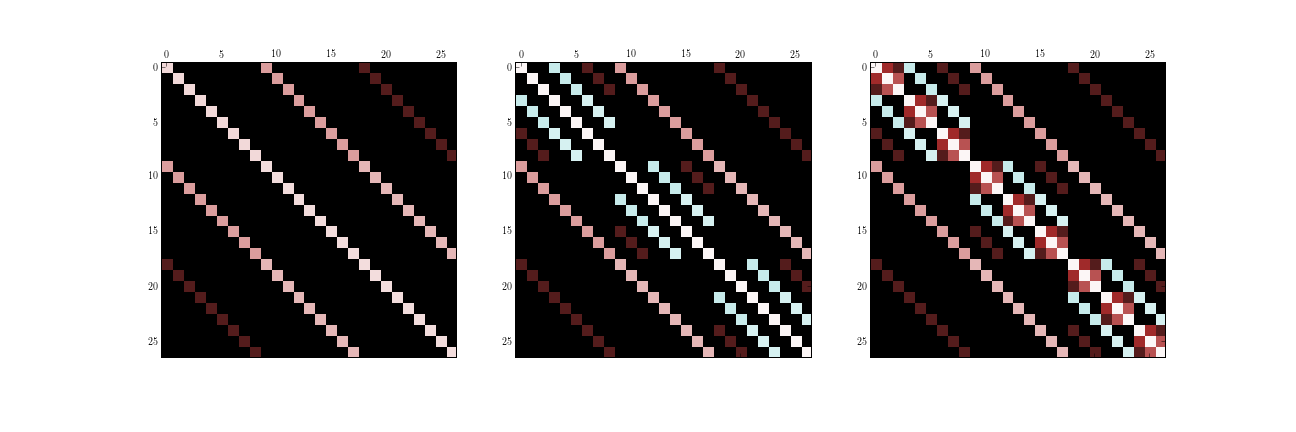
\includegraphics[width=\linewidth]{./fig/matrix_elements_1.png}
  \caption[Matrix elements example 1]{
  The plots show the matrices $\mat{F}$ consisting of the matrix elements $\Braket{\phi_{\vec{k}} | V | \phi_{\vec{l}}}$
  for $V = \frac{1}{2} x^2$ (left), $V = \frac{1}{2} \left(x^2 + y^2\right)$ (middle)
  and $V = \frac{1}{2} \left(x^2 + y^2 + z^2\right)$ (right). For an explanation of the colours, see appendix \ref{ch:color_code}.}
  \label{fig:matrix_elements_example1}
\end{figure}


\begin{figure}
  \centering
  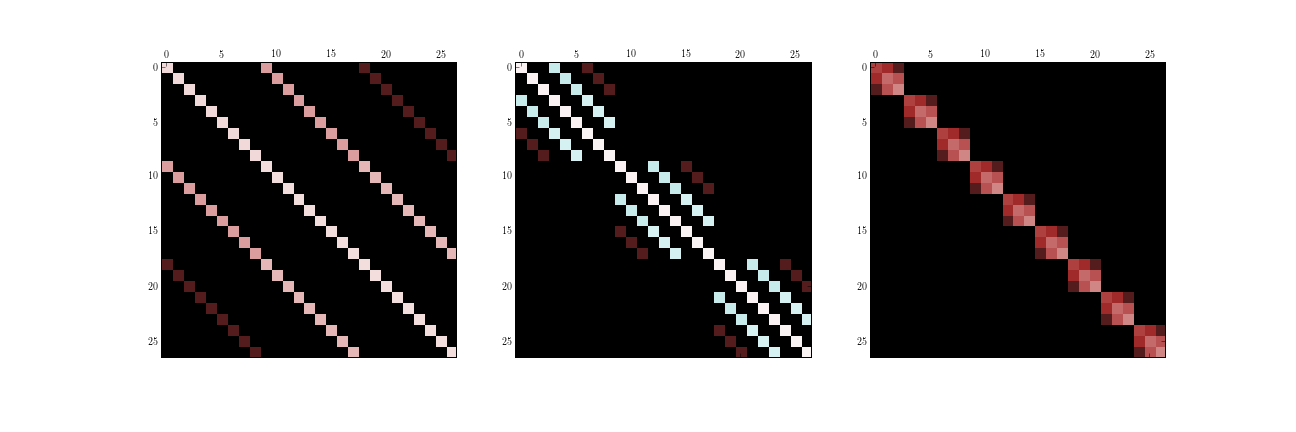
\includegraphics[width=\linewidth]{./fig/matrix_elements_2.png}
  \caption[Matrix elements example 2]{
  The plots show the matrices $\mat{F}$ consisting of the matrix elements $\Braket{\phi_{\vec{k}} | V | \phi_{\vec{l}}}$
  for $V = \frac{1}{2} x^2$ (left), $V = \frac{1}{2} y^2$ (middle)
  and $V = \frac{1}{2} z^2$ (right). For an explanation of the colours, see appendix \ref{ch:color_code}.}
  \label{fig:matrix_elements_example2}
\end{figure}

The block structures in the plots are due to the linearisation mapping $\mu_{\mathfrak{K}}$
and the dependence of $V$ on the variables $x$, $y$ and $z$.


\section{Computing norms of wavepackets}


In the following we want to compute the norm of a wavepacket $\Ket{\Psi}$.
This is the most simple observable or braket where the operator in between
the bra and the ket is just an identity. We start with:

\begin{align*}
  \|\Psi\|^2_{L^2} & = \Braket{\Psi | \Psi} \\
                   & = \sum_{i=0}^{N-1} \Braket{\Phi_i | \Phi_i} \\
                   & = \sum_{i=0}^{N-1} \| \Phi_i \|^2_{L^2} \,.
\end{align*}

Obviously the squared norm of the vector valued wavepacket is the sum of the
squared norms of its components. This is a pattern we will find several times more
when computing observables. In the general case however, the components may get
mixed up by the operator in the middle. Let's continue with calculating the norms
of an individual component which can be considered as a scalar wavepacket. Therefore
we also drop the index $i$ from above.

\begin{align*}
  \Braket{\Phi[\Pi] | \Phi[\Pi]} & = \Braket{ \exp\left(\frac{i S}{\varepsilon^2}\right)
                                              \sum_{\vec{k}\in\mathfrak{K}} c_{\vec{k}} \phi_{\vec{k}}[\Pi](\vec{x})
                                              |
                                              \exp\left(\frac{i S}{\varepsilon^2}\right)
                                              \sum_{\vec{l}\in\mathfrak{K}} c_{\vec{l}} \phi_{\vec{l}}[\Pi](\vec{x})
                                              } \\
  & = \exp\left(\frac{-i S}{\varepsilon^2}\right)\exp\left(\frac{i S}{\varepsilon^2}\right)
      \Braket{ \sum_{\vec{k}\in\mathfrak{K}} c_{\vec{k}} \phi_{\vec{k}}[\Pi](\vec{x})
               |
               \sum_{\vec{l}\in\mathfrak{K}} c_{\vec{l}} \phi_{\vec{l}}[\Pi](\vec{x})
             } \\
\intertext{The global phase cancels here and we get:}
  & = \sum_{\vec{k}\in\mathfrak{K}} \conj{c_{\vec{k}}} \sum_{\vec{l}\in\mathfrak{K}} c_{\vec{l}}
      \Braket{ \phi_{\vec{k}}[\Pi](\vec{x}) | \phi_{\vec{l}}[\Pi](\vec{x}) } \,.
\end{align*}

Now we can exploit the orthonormality condition $\Braket{ \phi_{\vec{k}} | \phi_{\vec{l}} } = \kron{\vec{k},\vec{l}}$
of the basis functions and arrive at:

\begin{equation}
  \|\Phi\|^2_{L^2} = \Braket{\Phi[\Pi] | \Phi[\Pi]} = \sum_{\vec{k}\in\mathfrak{K}} \conj{c_{\vec{k}}} c_{\vec{k}}
                   = \sum_{\vec{k}\in\mathfrak{K}} |c_{\vec{k}}|^2 \,.
\end{equation}


\section{Computing overlap integrals of wavepackets}


If we wanted to compute \emph{overlap integrals} between scalar wavepackets, then
the procedure is very similar but allows for less simplifications. Notice that
now the parameter set $\Pi$ of $\Phi[\Pi]$ can be and in general will be different.
To distinguish them we use $\Pi$ and $\Pi^\prime$.

\begin{align*}
  \Braket{\Phi[\Pi] | \Phi^\prime[\Pi^\prime]}
  & = \Braket{ \exp\left(\frac{i S}{\varepsilon^2}\right)
               \sum_{\vec{k}\in\mathfrak{K}} c_{\vec{k}} \phi_{\vec{k}}[\Pi](\vec{x})
               |
               \exp\left(\frac{i S^\prime}{\varepsilon^2}\right)
               \sum_{\vec{l}\in\mathfrak{K^\prime}} c^\prime_{\vec{l}} \phi_{\vec{l}}[\Pi^\prime](\vec{x})
              } \\
  & = \exp\left(\frac{-i S}{\varepsilon^2}\right)\exp\left(\frac{i S^\prime}{\varepsilon^2}\right)
      \Braket{ \sum_{\vec{k}\in\mathfrak{K}} c_{\vec{k}} \phi_{\vec{k}}[\Pi](\vec{x})
               |
               \sum_{\vec{l}\in\mathfrak{K^\prime}} c^\prime_{\vec{l}} \phi_{\vec{l}}[\Pi^\prime](\vec{x})
             } \\
\intertext{The global phase does not cancel here and we get:}
  & = \exp\left(\frac{-i S}{\varepsilon^2}\right)\exp\left(\frac{i S^\prime}{\varepsilon^2}\right)
      \sum_{\vec{k}\in\mathfrak{K}} \conj{c_{\vec{k}}} \sum_{\vec{l}\in\mathfrak{K^\prime}} c^\prime_{\vec{l}}
      \Braket{ \phi_{\vec{k}}[\Pi](\vec{x}) | \phi_{\vec{l}}[\Pi^\prime](\vec{x}) } \,.
\end{align*}

At the end of the day we get the following formula for the overlap of two scalar wavepackets:

\begin{equation}
  \Braket{\Phi[\Pi] | \Phi^\prime[\Pi^\prime]}
  =
  \exp\left(\frac{i}{\varepsilon^2}(S^\prime - S)\right)
  \sum_{\vec{k}\in\mathfrak{K}} \sum_{\vec{l}\in\mathfrak{K^\prime}} \conj{c_{\vec{k}}} c^\prime_{\vec{l}}
  \Braket{ \phi_{\vec{k}}[\Pi] | \phi_{\vec{l}}[\Pi^\prime] } \,.
\end{equation}

This is the most general formula for overlap integrals (which includes computation of norms).
We allowed for different Hagedorn parameter sets $\Pi$ and $\Pi^\prime$ as well as different
basis shapes $\mathfrak{K}$ and $\mathfrak{K}^\prime$. Hereby we conclude this section and
continue with the computation of energies in the next one.


\section{Computing energies of wavepackets}


To compute the energies of a wavepacket we start with the full Hamiltonian $\mat{H} = \mat{T} + \mat{V}(\vec{x})$.
Then the total energy of $\Ket{\Psi}$ is given by:

\begin{equation}
  E_{\text{total}} = \Braket{\Psi | \mat{H} | \Psi} \,.
\end{equation}

Next we split this braket into the kinetic energy and the potential energy contribution:

\begin{align*}
  E_{\text{total}} & = \Braket{\Psi | \mat{H} | \Psi}
                   & = \Braket{\Psi | \mat{T} | \Psi} + \Braket{\Psi | \mat{V}(\vec{x}) | \Psi}
                     = E_{\text{kinetic}} + E_{\text{potential}} \,.
\end{align*}

\subsection{Potential energy}

We start by computing the potential energy explicitly. Recall the definition of the
potential given in equation \eqref{eq:potential_matrix}. Plugging this matrix
$\mat{V}(\vec{x})$ into the braket above we get:

\begin{align*}
  E_{\text{potential}}
  & = \Braket{\Psi | \mat{V}(\vec{x}) | \Psi} \\
  & = \Braket{
    \begin{pmatrix}
      \Phi_0(\vec{x}) \\
      \vdots \\
      \Phi_{N-1}(\vec{x}) \\
    \end{pmatrix}
    |
    \begin{pmatrix}
      v_{0,0}(\vec{x})   & \cdots & v_{0,N-1}(\vec{x}) \\
      \vdots             &        & \vdots \\
      v_{N-1,0}(\vec{x}) & \cdots & v_{N-1,N-1}(\vec{x})
    \end{pmatrix}
    \begin{pmatrix}
      \Phi_0(\vec{x}) \\
      \vdots \\
      \Phi_{N-1}(\vec{x}) \\
    \end{pmatrix}
    } \\
  & = \Braket{
    \begin{pmatrix}
      \Phi_0(\vec{x}) \\
      \vdots \\
      \Phi_{N-1}(\vec{x}) \\
    \end{pmatrix}
    |
    \begin{pmatrix}
      \sum_{i=0}^{N-1} v_{0,i}(\vec{x}) \Phi_i(\vec{x}) \\
      \vdots \\
      \sum_{i=0}^{N-1} v_{N-1,i}(\vec{x}) \Phi_i(\vec{x}) \\
    \end{pmatrix}
    } \\
  & = \sum_{j=0}^{N-1} \sum_{i=0}^{N-1} \Braket{ \Phi_j(\vec{x}) | v_{j,i}(\vec{x}) \Phi_i(\vec{x}) }
\end{align*}

where we expressed the potential energy of the vector-valued wavepacket $\Ket{\Psi}$ by a sum
of potential energies of its components $\Phi_i$. This is a first step towards our goal.

If we want to compute the potential energy of the wavepacket on each energy surface $\lambda(\vec{x})$
then we have to do the calculation in the eigenbasis shown in equation \eqref{eq:eigenlevels_matrix}.
Because the matrix is diagonal now we can obtain a simplified version of the double sum above:

\begin{align}
  E_{\text{potential}} & = \Braket{\Psi|\mat{\Lambda}(\vec{x})|\Psi} \nonumber\\
                       & = \sum_{i=0}^{N-1} \Braket{ \Phi_i(\vec{x}) | \lambda_{i}(\vec{x}) \Phi_i(\vec{x}) }
\end{align}

where the braket $\Braket{ \Phi_i(\vec{x}) | \lambda_{i}(\vec{x}) \Phi_i(\vec{x}) }$ on the
last line is the potential energy of the part $\Phi_i$ of $\Ket{\Psi}$ residing
on the energy surface $\lambda_i(\vec{x})$. Of course we need to transform the
wavepacket $\Ket{\Psi}$ to the eigenbasis before we can apply the above formula.
How to do this is shown in section \ref{sec:basis_transformation_wp}. The integral
is then approximated by a high-order quadrature as shown at the beginning of this chapter.


\subsection{Kinetic energy}


From the chapter \ref{ch:fourier} we know that the kinetic operator $\mat{T}$ is block-diagonal
and does not couple the different components of $\Psi$. Hence we find that:

\begin{align*}
  E_{\text{kinetic}} & = \Braket{\Psi| \mat{T} |\Psi}
  = \Braket{
    \begin{pmatrix}
      \Phi_0(\vec{x}) \\
      \vdots \\
      \Phi_{N-1}(\vec{x}) \\
    \end{pmatrix}
    |
    \begin{pmatrix}
      T  & {}     & 0 \\
      {} & \ddots & {} \\
      0  & {}     & T
    \end{pmatrix}
    \begin{pmatrix}
      \Phi_0(\vec{x}) \\
      \vdots \\
      \Phi_{N-1}(\vec{x}) \\
    \end{pmatrix}
    } \\
  & = \sum_{i=0}^{N-1} \Braket{ \Phi_i(\vec{x}) | T | \Phi_i(\vec{x}) } \,.
\end{align*}

We can concentrate at the last braket including a scalar wavepacket $\Phi$ only. To take
the next step we bring to mind that $T$ actually is given by $T = -\frac{1}{2} \varepsilon^4 \Delta$
and therefore we have:

\begin{align*}
  \Braket{ \Phi(\vec{x}) | T | \Phi(\vec{x}) } & = \Braket{ \Phi(\vec{x}) | -\frac{1}{2} \varepsilon^4 \Delta | \Phi(\vec{x}) } \,.
\intertext{We split the operator into two parts by formally taking the square root of $T$:}
  & = \frac{1}{2} \Braket{ \Phi(\vec{x}) | (-i \varepsilon^2 \nabla)(-i \varepsilon^2 \nabla) | \Phi(\vec{x}) } \,.
\intertext{Then we put the two parts into the bra and the ket respectively}
  & = \frac{1}{2} \Braket{ +i \varepsilon^2 \nabla \Phi(\vec{x}) |-i \varepsilon^2 \nabla \Phi(\vec{x}) } \\
  & = \frac{1}{2} \|-i \varepsilon^2 \nabla \Phi(\vec{x})\|^2 \,.
\end{align*}

The braket simply expresses the squared norm of $-i \varepsilon^2 \nabla \Phi$. If we want to compute
this norm we need to know how the operator $y \assign -i \varepsilon^2 \nabla$ acts on the wavepacket.
If we remember correctly, we have done all necessary computation already in section \ref{sec:gradient_computation}.


\section{Basis transformations}
\label{sec:basis_transformation_wp}


This is a last small section before we can go to the time propagation algorithm
for wavepackets in the next chapter. In this part we describe the basis
transformation of vectorial wavepackets $\Ket{\Psi}$ in detail. Recall the
definition of the eigenbasis from \eqref{eq:eigenlevels_matrix} and the basis
transformation from \eqref{eq:eigentransformation}. Then the basis transformation
of our wavepacket $\Ket{\Psi}$ from and to the canonical basis hence looks like:

\begin{equation} \label{eq:basis_trafos}
\begin{split}
  \Ket{\Psi_\text{canonical}} & = \mat{M}(\vec{x}) \Ket{\Psi_\text{eigen}} \\
  \Ket{\Psi_\text{eigen}}     & = \mat{M}\inv(\vec{x}) \Ket{\Psi_\text{canonical}} = \mat{M}\H(\vec{x}) \Ket{\Psi_\text{canonical}}
\end{split}
\end{equation}

and we exploited the fact that all eigenvectors are orthonormal. We can write a
more explicit version of $\mat{M}$ (we do not reuse \ref{eq:eigentransformation_matrix}
for notational reasons):

\begin{equation*}
  \mat{M}(\vec{x}) \assign
  \begin{pmatrix}
    m_{0,0}(\vec{x})   & \cdots & m_{0,N-1}(\vec{x}) \\
    \vdots             &        & \vdots \\
    m_{N-1,0}(\vec{x}) & \cdots & m_{N-1,N-1}(\vec{x})
  \end{pmatrix} \,.
\end{equation*}

From this the application of $\mat{M}$ to $\Ket{\Psi}$ becomes obvious:

\begin{align*}
  \mat{M}(\vec{x}) \Ket{\Psi(\vec{x}} & =
  \begin{pmatrix}
    m_{0,0}(\vec{x})   & \cdots & m_{0,N-1}(\vec{x}) \\
    \vdots             &        & \vdots \\
    m_{N-1,0}(\vec{x}) & \cdots & m_{N-1,N-1}(\vec{x})
  \end{pmatrix}
  \begin{pmatrix}
    \Phi_0(\vec{x}) \\
    \vdots \\
    \Phi_{N-1}(\vec{x})
  \end{pmatrix} \\
  & =
  \begin{pmatrix}
    m_{0,0}(\vec{x}) \Phi_0(\vec{x}) + \cdots + m_{0,N-1}(\vec{x}) \Phi_{N-1}(\vec{x}) \\
    \vdots \\
    m_{N-1,0}(\vec{x}) \Phi_0(\vec{x}) + \cdots + m_{N-1,N-1}(\vec{x}) \Phi_{N-1}(\vec{x})
  \end{pmatrix} \\
  & =
  \begin{pmatrix}
    \Phi_0^\prime(\vec{x}) \\
    \vdots \\
    \Phi_{N-1}^\prime(\vec{x})
  \end{pmatrix}
  = \Ket{\Psi^\prime} \,.
\end{align*}


\subsection{Transformation of homogeneous wavepackets}


Next we dig deeper and take a detailed look at a single row $j$ of the above matrix
vector product:

\begin{align*}
  m_{j,0} \Phi_0 + \cdots + m_{j,N-1} \Phi_{N-1} & =
  m_{j,0} \sum_{\vec{k}\in\mathfrak{K}} c_{\vec{k}}^0 \phi_{\vec{k}} + \cdots
  + m_{j,N-1} \sum_{\vec{k}\in\mathfrak{K}} c_{\vec{k}}^{N-1} \phi_{\vec{k}} \\
  & =
  \sum_{\vec{k}\in\mathfrak{K}} m_{j,0}  c_{\vec{k}}^0 \phi_{\vec{k}} + \cdots
  + \sum_{\vec{k}\in\mathfrak{K}} m_{j,N-1} c_{\vec{k}}^{N-1} \phi_{\vec{k}} \\
  & =
  \sum_{\vec{k}\in\mathfrak{K}} \left( m_{j,0}  c_{\vec{k}}^0 + \cdots + m_{j,N-1}  c_{\vec{k}}^{N-1} \right) \phi_{\vec{k}} \\
  & =
  \sum_{\vec{k}\in\mathfrak{K}} \underbrace{\sum_{l=0}^{N-1} m_{j,l}  c_{\vec{k}}^l }_{c_{\vec{k}}^\prime} \phi_{\vec{k}}
  = \sum_{\vec{k}\in\mathfrak{K}} c_{\vec{k}}^\prime \phi_{\vec{k}} = \Phi_{j}^\prime \,.
\end{align*}

This is a simple calculation but with a big potential for errors. But we are almost
done with the most error-prone parts. Since the new coefficients $c_{\vec{k}}^\prime$
depend on $\vec{x}$ through the entries $m_{j,l}(\vec{x})$ of $\mat{M}$ we need
to project on the subspace spanned by our basis functions $\phi_{\vec{k}}$.
This works as follows. First we compute new coefficients:

\begin{equation*}
  d_{\vec{p}}^j \assign \Braket{ \phi_{\vec{p}} | \Phi_{j}^\prime} \quad \forall \vec{p} \in \mathfrak{K}
\end{equation*}

and then we build the transformed scalar and vectorial wavepackets step by step as:

\begin{equation*}
  \Phi_j^{\prime\prime}(\vec{x}) = \sum_{\vec{k}\in\mathfrak{K}} d_{\vec{k}}^j \phi_{\vec{k}}(\vec{x})
  \quad\text{and finally}\quad
  \Ket{\Psi^{\prime\prime}} =
  \begin{pmatrix}
    \Phi_0^{\prime\prime} \\
    \vdots \\
    \Phi_{N-1}^{\prime\prime}
  \end{pmatrix} \,.
\end{equation*}

In principle we are done now. One very last thing to show is the efficient
computation of the new coefficients $d_{\vec{p}}^j$. It seems to be complicated
but in fact is very simple once we look at a coarser picture. The first step
is to rewrite:

\begin{align*}
  d_{\vec{p}}^j & \assign \Braket{ \phi_{\vec{p}} | \Phi_{j}^\prime}
  = \Braket{ \phi_{\vec{p}} | \sum_{\vec{k}\in\mathfrak{K}} \sum_{l=0}^{N-1} m_{j,l}  c_{\vec{k}}^l \phi_{\vec{k}} } \\
  & = \sum_{\vec{k}\in\mathfrak{K}} \sum_{l=0}^{N-1} \Braket{ \phi_{\vec{p}} | m_{j,l} \phi_{\vec{k}} } c_{\vec{k}}^l
\end{align*}

where we obtained $|\mathfrak{K}|^2$ matrix elements of the form:

\begin{equation*}
  \Braket{ \phi_{\vec{p}} | m_{j,l} | \phi_{\vec{k}} }
  = \idotsint_{\mathbb{R}^D} \conj{\phi_{\vec{p}}(\vec{x})} \, m_{j,l}(\vec{x}) \, \phi_{\vec{k}}(\vec{x}) \mathrm{dx} \,.
\end{equation*}

Computing every single $d_{\vec{p}}^j$ individually would be very cumbersome and
inefficient too. We can do better by noticing that it is possible to rearrange
the above expression into a matrix vector product form. Next we stack all
$c_{\vec{k}}$ and $d_{\vec{p}}$ into long column vectors of size $|\mathfrak{K}|$.
The order is given according to $\mu_{\mathfrak{K}}$. We gather all matrix
elements and build the following matrix $\mat{F_{j,l}} \in \mathbb{C}^{|\mathfrak{K}| \times |\mathfrak{K}|}$:

\begin{equation*}
  \mat{F_{j,l}} \assign
  \begin{pmatrix}
    {}     & \vdots                                               & {} \\
    \cdots & \Braket{ \phi_{\vec{p}} | m_{j,l} | \phi_{\vec{k}} } & \cdots \\
    {}     & \vdots                                               & {}
  \end{pmatrix}
\end{equation*}

where we put the integral $\Braket{ \phi_{\vec{p}} | m_{j,l} | \phi_{\vec{k}} }$
at position $\left(\mu(\vec{p}), \mu(\vec{k})\right)$.

Therefore we can now compute $d_{\vec{p}}^l$ for all $\vec{p} \in \mathfrak{K}$
at once by:

\begin{equation*}
  \begin{pmatrix}
    d_{0}^j \\
    \vdots \\
    d_{|\mathfrak{K}|}^j \\
  \end{pmatrix}
  = \sum_{l=0}^{N-1}
  \begin{pmatrix}
    {}     & \vdots                                               & {} \\
    \cdots & \Braket{ \phi_{\vec{p}} | m_{j,l} | \phi_{\vec{k}} } & \cdots \\
    {}     & \vdots                                               & {}
  \end{pmatrix}
  \begin{pmatrix}
    c_{0}^l \\
    \vdots \\
    c_{|\mathfrak{K}|}^l \\
  \end{pmatrix}
\end{equation*}

and thereby express the new coefficients $\vec{d^j}$ of our transformed component
$\Phi_j$ by a sum of matrix vector products. This can be done very efficiently.
Aiming for an even coarser view we can stack the computations for all $j \in (0,\ldots, N-1)$.
First we build the block matrix $\mat{F} \in \mathbb{C}^{N|\mathfrak{K}| \times N|\mathfrak{K}|}$:

\begin{equation*}
  \mat{F} \assign
  \begin{pmatrix}
    \mat{F_{0,0}}   & \cdots        & \mat{F_{0, N-1}} \\
    \vdots          & \mat{F_{j,l}} & \vdots \\
    \mat{F_{N-1,0}} & \cdots        & \mat{F_{N-1, N-1}} \\
  \end{pmatrix}
\end{equation*}

The matrix can be computed efficiently by algorithm \ref{al:build_block_matrix_homog}.
Using the same partition scheme we stack the coefficient vectors $\vec{d^j}$ and
$\vec{c^j}$ for all $j$ into even longer column vectors of size $N |\mathfrak{K}|$
(we assume each component having the same basis shape):

\begin{align*}
  \vec{c} \assign \left( \vec{c^0} , \ldots , \vec{c^{N-1}} \right)\T
  \quad \text{and} \quad
  \vec{d} \assign \left( \vec{d^0} , \ldots , \vec{d^{N-1}} \right)\T
\end{align*}

At the end of the day we can express the whole basis transformation as given in
equation \eqref{eq:basis_trafos} by a simple matrix vector product. For the
transformation to the eigenbasis we get:

\begin{equation}
  \vec{c}_{\,\text{eigen}} = \mat{F} \vec{c}_{\,\text{canonical}}
\end{equation}

and we only need to split up $\vec{c}$ according to the partition used.
For the opposite transformation to the canonical basis we can write:

\begin{equation}
  \vec{c}_{\,\text{canonical}} = \mat{F}\H \vec{c}_{\,\text{eigen}}
\end{equation}

since $\mat{F}$ is unitary. The only point not shown here is the detailed
computation of the matrix elements of $\mat{F_{j,l}}$. This is not complicated
but a little bit tricky to do efficiently. The integrals are of course approximated
by the quadrature rules shown earlier in this chapter. The whole process is presented
in \cite{B_bachelor_thesis}.


\subsection{Transformation of inhomogeneous wavepackets}


In the case of inhomogeneous wavepackets the whole basis transformation process
works similar. There are just a few points where we have to be more general.
Again we first look at a single row $j$ of $\Ket{\Psi^\prime} = \mat{M} \Ket{\Psi}$.
Main point here is to take into account the possibly different parameter sets $\Pi_j$
and basis shapes $\mathfrak{K}_j$ of each component:

\begin{align*}
       & m_{j,0} \Phi_0[\Pi_0] + \cdots + m_{j,N-1} \Phi_{N-1}[\Pi_{N-1}] \\
  = \, & \sum_{\vec{k}\in\mathfrak{K}_0} m_{j,0}  c_{\vec{k}}^0 \phi_{\vec{k}}[\Pi_0] + \cdots
         + \sum_{\vec{k}\in\mathfrak{K}_{N-1}} m_{j,N-1} c_{\vec{k}}^{N-1} \phi_{\vec{k}}[\Pi_{N-1}] \\
  = \, & \sum_{l=0}^{N-1} \sum_{\vec{k}\in\mathfrak{K}_l} m_{j,l} \, c_{\vec{k}}^l \, \phi_{\vec{k}}[\Pi_l] \,.
\end{align*}

Now we enter the projection step with this last expression giving:

\begin{align*}
  d_{\vec{p}}^j & \assign \Braket{ \phi_{\vec{p}}[\Pi_j] | \sum_{l=0}^{N-1} \sum_{\vec{k}\in\mathfrak{K}_l} m_{j,l} \, c_{\vec{k}}^l \, \phi_{\vec{k}}[\Pi_l] } \\
                & = \sum_{l=0}^{N-1} \sum_{\vec{k}\in\mathfrak{K}_l}
                    \Braket{\phi_{\vec{p}}[\Pi_j] | m_{j,l} | \phi_{\vec{k}}[\Pi_l]} c_{\vec{k}}^l \,.
\end{align*}

For these brakets on the last line we have to use the inhomogeneous quadrature
rule as the basis functions in the bra and the ket can have different parameter
sets $\Pi$. The matrix $\mat{F_{j,l}}$ is of size $|\mathfrak{K}_j| \times |\mathfrak{K}_l|$
and not necessarily square. (Theoretically we could have used different basis shapes
$\mathfrak{K}_j$ per component $\Phi_j$ already in the homogeneous case.)

\begin{equation*}
  \mat{F_{j,l}} \assign
  \begin{pmatrix}
    {}     & \vdots                                                           & {} \\
    \cdots & \Braket{\phi_{\vec{p}}[\Pi_j] | m_{j,l} | \phi_{\vec{k}}[\Pi_l]} & \cdots \\
    {}     & \vdots                                                           & {}
  \end{pmatrix}
\end{equation*}

The block matrix $\mat{F}$ is of shape $\sum_{i=0}^{N-1} |\mathfrak{K}_i| \times \sum_{i=0}^{N-1} |\mathfrak{K}_i|$
and obviously square. (This is a requirement because the transformation mapping
should be bijective.) We can compute this matrix by algorithm \ref{al:build_block_matrix_inhomog}.
Everything else works exactly the same as in the homogeneous case.

\chapter{Wavepacket Propagation}
\label{ch:wavepacket_propagation}


This last theoretical chapter is about time propagation of semi-classical
wavepackets. The last remaining missing piece of this puzzle is a good scheme
for time propagation of semi-classical Hagedorn wavepackets. Such an algorithm was
first described in \cite{FGL_semiclassical_dynamics} for the adiabatic one-level
case. The generalisation to multiple energy levels was done in \cite{B_bachelor_thesis}
but for one space dimension only. These results were published in \cite{BGH_nonadibatic_algorithms}.

In this chapter we review this algorithm once more and show a generalisation
to several energy levels in an arbitrary dimensional space.


\section{Time propagation of Hagedorn wavepackets}


The first step is to consider the free particle Schrödinger equation which
contains only the kinetic operator $T$ and $V \equiv 0$:

\begin{equation*}
  i \varepsilon^2  \pdiff{\Psi}{t} = -\frac{1}{2} \varepsilon^4 \Delta \Psi \,.
\end{equation*}

The proposition 2.1 of \cite{FGL_semiclassical_dynamics} tells us that a Hagedorn wavepacket
$\Phi[\Pi]$ of the form \eqref{eq:scalar_wavepacket} solves the free Schrödinger
equation with the following time evolution of its parameter set $\Pi(t)$:

\begin{equation} \label{eq:update_scheme_kin}
\begin{split}
  \vec{q}(t) & = \vec{q}(0) + t \, \mat{M}\inv \vec{p}(0) \\
  \mat{Q}(t) & = \mat{Q}(0) + t \, \mat{M}\inv \mat{P}(0) \\
  S(t) & = S(0) + \frac{1}{2}t \, \vec{p}(0)\T \mat{M}\inv \vec{p}(0)
\end{split}
\end{equation}

where $\vec{p}(t) = \vec{p}(0)$ and $\mat{P}(t) = \mat{P}(0)$ remain unchanged.
Also unchanged are the coefficients $\{c_{\vec{k}}\}_{\vec{k} \in \mathfrak{K}}$
of $\Phi$. The matrix $\mat{M}$ is the mass scaling matrix. It is set to the
identity if nothing else is written. For details see \cite[equation 2.8]{FGL_semiclassical_dynamics}.
A free particle is not that interesting. The important point is that we can
solve its quantum equation of motion by only evolving the parameters $\Pi(t)$
using the simple update scheme above.

Next we consider the potential equation lacking the kinetic part:

\begin{equation*}
  i \varepsilon^2  \pdiff{\Psi}{t} = U(\vec{x}) \Psi \,.
\end{equation*}

For a first approach we assume $U(\vec{x})$ to be quadratic at most. The
proposition 2.2 of \cite{FGL_semiclassical_dynamics} gives us another set of update rules
for $\Pi(t)$:

\begin{equation} \label{eq:update_scheme_pot}
\begin{split}
  \vec{p}(t) & = \vec{p}(0) - t \, \nabla U(\vec{q}(0)) \\
  \mat{P}(t) & = \mat{P}(0) - t \, \nabla^2 U(\vec{q}(0)) \mat{Q}(0) \\
  S(t) & = S(0) - t \, U(\vec{q}(0))
\end{split}
\end{equation}

and $\vec{q}(t) = \vec{q}(0)$ and $\mat{Q}(t) = \mat{Q}(0)$. In this case the
coefficients $\{c_{\vec{k}}\}_{\vec{k} \in \mathfrak{K}}$ are left alone. Using
the formulae from both sets \eqref{eq:update_scheme_kin} and \eqref{eq:update_scheme_pot}
together we can solve the time dependent harmonic oscillator. All we have to do is to
propagate in time the parameter set $\Pi(t)$ of $\Phi[\Pi]$. In the whole
process we never touch or change the coefficients $\{c_{\vec{k}}\}_{\vec{k} \in \mathfrak{K}}$.
This is the reason that makes this time propagation scheme extraordinarily
efficient. But this is not really astonishing given that the basis functions
$\phi_{\vec{k}}$ are just generalised eigenstates of the harmonic oscillator.
(For more details see the paper \cite{H_ladder_operators}).

Our next step aims for handling almost arbitrary potentials. But dropping the
restriction of $U$ being quadratic provides us with several new hurdles.
Assume the potential $V(\vec{x})$ is not quadratic anymore. We can always split
$V$ into a quadratic part $U$ and the non-quadratic remainder $W$:

\begin{equation*}
  V(\vec{x}) = U(\vec{x}) + W(\vec{x}) \,.
\end{equation*}

This is done by a simple Taylor expansion of $V(\vec{x})$ around a point
\footnote{It's not a coincidence that we call the expansion point $\vec{q}$ here.}
$\vec{q}$ giving:

\begin{align*}
  U(\vec{x}) & = V(\vec{q}) + \nabla V(\vec{q}) (\vec{x}-\vec{q})
                 + \frac{1}{2} (\vec{x}-\vec{q})\T \nabla^2 V(\vec{q}) (\vec{x}-\vec{q}) \\
  W(\vec{x}) & = V(\vec{x}) - U(\vec{x}) \,.
\end{align*}

This expansion allows us to focus on $W(\vec{x})$ solely while assuming that
$U(\vec{x})$ is perfectly handled by \eqref{eq:update_scheme_pot}. We look at
the potential equation:

\begin{equation*}
  i \varepsilon^2  \pdiff{\Psi}{t} = W(\vec{x}) \Psi
\end{equation*}

once more but this time using the non-quadratic remainder part $W(\vec{x})$.
Since $W$ can be arbitrarily complicated there is no hope to solve this
equation analytically by a simple scheme as we did before. The trick is to
perform a Galerkin approximation to solve this equation. To do this we need
a Hilbert space of test functions $v(\vec{x})$ defined by:

\begin{equation}
  \mathcal{M} \assign \left\{ v \in \mathrm{L}^2(\mathbb{R}^D) \colon
                              v(\vec{x}) \assign \sum_{\vec{k}\in\mathfrak{K}}
                                                 c_{\vec{k}} \phi_{\vec{k}}[\Pi](\vec{x})
                         \,, c_{\vec{k}} \in \mathbb{C}
                      \right\} \,.
\end{equation}

At this point we may repeat that $\phi_{\vec{k}}$ constitutes a (complete) basis
for $\mathrm{L}^2(\mathbb{R}^D)$. The Galerkin approximation (see section 2.4 of
\cite{FGL_semiclassical_dynamics}) can then be written as:

\begin{quotation}
  \noindent
  At every time $t$ determine $\partial_t u \in \mathcal{M}$ such that
  \begin{equation*}
    \forall \vec{k} \in \mathfrak{K} \quad \langle \phi_{\vec{k}}, (i\varepsilon^2\partial_t -W) u \rangle = 0
  \end{equation*}
  with $u \in \mathcal{M}$.
\end{quotation}

This integral can now be split like:

\begin{align*}
  0 & = \langle \phi_{\vec{k}}, (i\varepsilon^2\partial_t -W) u \rangle \\
    & = \langle \phi_{\vec{k}}, i\varepsilon^2\partial_t u \rangle - \langle \phi_{\vec{k}}, W u \rangle
\end{align*}

and the solution $u$ can in turn be replaced by its basis expansion:

\begin{equation*}
  \langle \phi_{\vec{k}}, i\varepsilon^2 \partial_t
                          \sum_{\vec{l}\in\mathfrak{K}} c_{\vec{l}} \phi_{\vec{l}}
  \rangle -
  \langle \phi_{\vec{k}}, W
                          \sum_{\vec{l}\in\mathfrak{K}} c_{\vec{l}} \phi_{\vec{l}}
  \rangle = 0 \,.
\end{equation*}

Next we carry out the differentiation $\partial_t c_{\vec{l}} \phi_{\vec{l}}$.
We know that $c_{\vec{l}}(t)$ depends only on time and $\phi_{\vec{l}}[\Pi](\vec{x})$
depends only on space (ignoring the time dependence of $\Pi$) and whence we get:

\begin{equation*}
  \partial_t c_{\vec{l}} \phi_{\vec{l}} = \dot{c_{\vec{l}}} \phi_{\vec{l}} \,.
\end{equation*}

Plugging this into the integrals above we obtain:

\begin{equation*}
  \langle \phi_{\vec{k}}, i\varepsilon^2
                          \sum_{\vec{l}\in\mathfrak{K}} \dot{c_{\vec{l}}} \phi_{\vec{l}}
  \rangle -
  \langle \phi_{\vec{k}}, W
                          \sum_{\vec{l}\in\mathfrak{K}} c_{\vec{l}} \phi_{\vec{l}}
  \rangle = 0
\end{equation*}

and pulling out the summations and constants yields:

\begin{equation*}
  i\varepsilon^2 \sum_{\vec{l}\in\mathfrak{K}} \dot{c_{\vec{l}}}
  \langle \phi_{\vec{k}}, \phi_{\vec{l}} \rangle
  -
  \sum_{\vec{l}\in\mathfrak{K}} c_{\vec{l}}
  \langle \phi_{\vec{k}}, W \phi_{\vec{l}} \rangle
  = 0 \,.
\end{equation*}

The first integral vanishes by orthonormality of the basis functions and what
remains is:

\begin{equation*}
  i\varepsilon^2 \dot{c_{\vec{k}}}
  =
  \sum_{\vec{l}\in\mathfrak{K}} c_{\vec{l}}
  \langle \phi_{\vec{k}}, W \phi_{\vec{l}} \rangle
  \quad \forall \vec{k} \in \mathfrak{K} \,.
\end{equation*}

We can stack all the $|\mathfrak{K}|$ equations and get the following system
of coupled ordinary differential equations:

\begin{equation*}
  i\varepsilon^2
  \begin{pmatrix}
    \vdots \\
    \dot{c_{\vec{k}}} \\
    \vdots
  \end{pmatrix}
  =
  \begin{pmatrix}
    {}     & \vdots                                  & {} \\
    \cdots & \dotp{\phi_{\vec{k}}}{W \phi_{\vec{l}}} & \cdots \\
    {}     & \vdots                                  & {}
  \end{pmatrix}
  \begin{pmatrix}
    \vdots \\
    c_{\vec{l}} \\
    \vdots
  \end{pmatrix}
\end{equation*}

or in more compact matrix notation:

\begin{equation}
  \dot{\vec{c}} = -\frac{i}{\varepsilon^2} \mat{F} \vec{c} \,.
\end{equation}

The solution of this system is trivially given by:

\begin{equation} \label{eq:update_scheme_coeff}
  \vec{c}(t) = \exp\left(-\frac{i}{\varepsilon^2} t \mat{F}\right) \vec{c}(0) \,.
\end{equation}

This was the last missing bit for the time propagation of scalar wavepackets
$\Ket{\Phi}$ inside arbitrarily shaped potentials $V(\vec{x})$. In algorithm
\ref{al:tp_wave_packets_scalar} we assembled all the pieces and provide a pseudo
code of the implementation.

\begin{algorithm}
\caption{Time propagation of scalar wavepackets $\Ket{\Phi}$}
\label{al:tp_wave_packets_scalar}
\begin{algorithmic}
  \REQUIRE A semi-classical wavepacket $\Ket{\Phi\ofs{\vec{x},t}}$
  \REQUIRE The Hagedorn parameter set $\Pi$ and the coefficients $\{c_{\vec{k}}\}_{\vec{k}\in\mathfrak{K}}$
  \REQUIRE The basis shape $\mathfrak{K}$ and the mapping $\mu_{\mathfrak{K}}$
  \REQUIRE The time step $\tau$
  \STATE // Propagate with the kinetic operator
  \STATE $\vec{q} \assign \vec{q} + \frac{\tau}{2} \mat{M}\inv \vec{p}$
  \STATE $\mat{Q} \assign \mat{Q} + \frac{\tau}{2} \mat{M}\inv \mat{P}$
  \STATE $S \assign S + \frac{\tau}{4} \vec{p}\T \mat{M}\inv \vec{p}$
  \STATE // Propagate with the local quadratic potential
  \STATE $\vec{p} \assign \vec{p} - \tau \, \nabla V\ofs{\vec{q}}$
  \STATE $\mat{P} \assign \mat{P} - \tau \, \nabla^2 V\ofs{\vec{q}} \mat{Q}$
  \STATE $S \assign S - \tau \, V\ofs{\vec{q}}$
  \STATE // Propagate with the non-quadratic remainder $W$
  \STATE // Assemble the matrix $\mat{F}$
  \STATE $\mat{F}_{\mu(\vec{k}),\mu(\vec{l})} \assign
          \Braket{\phi_{\vec{k}} | W\ofs{\vec{x}} | \phi_{\vec{l}}} \quad \forall \vec{k}, \vec{l} \in \mathfrak{K}$
  \STATE // And propagate the coefficients
  \STATE $\vec{c} \assign \exp\ofs{-\tau \frac{i}{\varepsilon^2} \mat{F}} \vec{c}$
  \STATE // Propagate with the kinetic operator again
  \STATE $\vec{q} \assign \vec{q} + \frac{\tau}{2} \mat{M}\inv \vec{p}$
  \STATE $\mat{Q} \assign \mat{Q} + \frac{\tau}{2} \mat{M}\inv \mat{P}$
  \STATE $S \assign S + \frac{\tau}{4} \vec{p}\T \mat{M}\inv \vec{p}$
  \RETURN $\Ket{\Phi\ofs{\vec{x},t+\tau}}$
\end{algorithmic}
\end{algorithm}


\section{Vector valued wavepackets}


In the last section we reviewed the time propagation algorithm for scalar semi-classical
wavepackets $\Ket{\Phi}$ or equivalently for potentials with a single energy level only.
For simulations in the non-adiabatic case we need an extended version that handles
vectorial wavepackets $\Ket{\Psi}$ as defined in \eqref{eq:vectorial_wavepacket_hom}
and \eqref{eq:vectorial_wavepacket_inhom}. We examine the case of homogeneous
wavepackets first. This has mainly two reasons, namely homogeneous wavepackets
play a more important role in practical simulations and we can show the important
concepts easier while the inhomogeneous case can be treated by simple generalisation
later.


\subsection{Homogeneous wavepacket propagation}


As we defined in \eqref{eq:vectorial_wavepacket_hom} a homogeneous wavepacket
$\Psi$ consists of $N$ components $\Phi_i$ all sharing the same parameter set
$\Pi$. This set of parameters is propagated by the same rules as in the scalar
case. The propagation of $\Pi$ has to take place in the eigenbasis of $\mat{V}$
where the energy levels $\lambda_i$ decouple. We need to choose one of these
levels $\lambda_i(\vec{x})$ which then governs the propagation of $\Pi$ and
plays the role of $V$ in the scalar case. We denote this particular level
by $\lambda_{\chi}$ and call $\chi \in [0, \ldots, N-1]$ the \emph{characteristic
component index}. Then we apply the usual splitting into quadratic part
and non-quadratic remainder. Formally we write:

\begin{align*}
  u_\chi(\vec{x}) & = \lambda_\chi(\vec{x}) + \nabla \lambda_\chi(\vec{q}) (\vec{x}-\vec{q})
                      + \frac{1}{2} (\vec{x}-\vec{q})\T \nabla^2 \lambda_\chi(\vec{q}) (\vec{x}-\vec{q}) \\
  w_\chi(\vec{x}) & = \lambda_\chi(\vec{x}) - u_\chi(\vec{x}) \,.
\end{align*}

This is sufficient for time propagation of $\Pi$ but not for the Galerkin step
where we propagate the coefficients $\{c_{\vec{k}}\}_{\vec{k} \in \mathfrak{K}}$.
There we need a splitting of the full matrix $\mat{V}(\vec{x}) = \mat{U}(\vec{x}) + \mat{W}(\vec{x})$
into quadratic part $\mat{U}(\vec{x})$ and remainder $\mat{W}(\vec{x})$ such that:

\begin{equation*}
  \mat{V} =
  \begin{pmatrix}
    u_\chi & {}     & {} \\
    {}     & \ddots & {} \\
    {}     &        & u_\chi
  \end{pmatrix}
  +
    \begin{pmatrix}
    v_{0,0} - u_\chi & \cdots & v_{0,N-1} \\
    \vdots           & \ddots & \vdots \\
    v_{N-1,0}        & \cdots & v_{N-1,N-1} - u_\chi
  \end{pmatrix} \,.
\end{equation*}

We will need $\mat{W}$ for building the matrix $\mat{F}$ later. Notice that up
to now we did not mix the different components $\Phi_i$. This only happens
during propagation of the coefficients. For this we stack the coefficients
$\{c_{\vec{k}}^i\}_{\vec{k} \in \mathfrak{K}_i}$ of all components $\Phi_i$
into a long column vector $\vec{c}$:

\begin{equation*}
  \vec{c} \assign
  \begin{pmatrix}
    \cdots & c_{\vec{k}}^0 & \cdots & | & \cdots & | & \cdots & c_{\vec{k}}^{N-1} & \cdots
  \end{pmatrix}
  \T
\end{equation*}

of length $\sum_{i=0}^{N-1} |\mathfrak{K}_i|$ or $N |\mathfrak{K}|$ if all
components have a basis shape of same size. Then we build the $\mat{F}$ matrix
for use in equation \eqref{eq:update_scheme_coeff}. Obviously it must have the
following block structure:

\begin{equation*}
  \mat{F} \assign
  \begin{pmatrix}
    \mat{F_{0,0}}   & \cdots        & \mat{F_{0, N-1}} \\
    \vdots          & \mat{F_{i,j}} & \vdots \\
    \mat{F_{N-1,0}} & \cdots        & \mat{F_{N-1, N-1}} \\
  \end{pmatrix}
\end{equation*}

and each block is of the form:

\begin{equation*}
  \mat{F_{i,j}} \assign
    \begin{pmatrix}
    {}     & \vdots                                               & {} \\
    \cdots & \Braket{ \phi_{\vec{k}} | \mat{W}_{i,j} | \phi_{\vec{l}} } & \cdots \\
    {}     & \vdots                                               & {}
  \end{pmatrix}
\end{equation*}

for $\vec{k} \in \mathfrak{K}_i$ and $\vec{l} \in \mathfrak{K}_j$. These blocks
are not necessarily square but the matrix $\mat{F}$ always is. (Compare this
to the matrices used for the basis transformation of wavepackets.)

Algorithm \ref{al:build_block_matrix_homog} gives pseudo code for the computation
of $\mat{F}$ given a quadrature rule, the remainder $\mat{W}$ and the homogeneous
wavepacket $\Psi[\Pi]$. The time propagation then is summarised in algorithm
\ref{al:tp_wave_packets_homog}.


\begin{algorithm}
\caption{Build the homogeneous block matrix $\mat{F} \assign \left(\mat{F_{r,c}}\right)_{r,c}$}
\label{al:build_block_matrix_homog}
\begin{algorithmic}
  \REQUIRE A homogeneous wavepacket $\Psi$ with parameter set $\Pi$
  \REQUIRE The basis shape $\mathfrak{K}_i$ of each component $\Phi_i$ of $\Psi$, $i = 0,\ldots, N-1$
  \REQUIRE A $N \times N$ matrix $\mat{W}(\vec{x})$ of scalar functions $w_{r,c}(\vec{x})$
  \REQUIRE A quadrature rule $(\vec{\gamma}_j, \omega_j)$ with $R$ node-weight pairs
  \STATE // Initialise $\mat{F}$ as the zero-matrix
  \STATE $\eta \assign \sum_{i=0}^{N-1} |\mathfrak{K}_i|$
  \STATE $\mat{F} \in \mathbb{C}^{\eta \times \eta}, \quad \mathbf{F} \assign \mathbf{0}$
  \STATE // Transform the quadrature nodes according to \eqref{eq:transformed_qr_nodes}
  \STATE $\vec{\gamma}_j^\prime = \vec{q} + \varepsilon \, \mat{Q} \, \vec{\gamma}_j \quad j = 0, \ldots R-1$
  \STATE // Evaluate the basis functions of each component $\Phi_i$ with algorithm \ref{al:eval_phi_basis}
  \FOR{$i = 0$ \TO $i = N-1$}
    \STATE $\mat{B_i} \assign \mathbf{evaluate\_basis\_at}[\Phi_i]\left(\left(\vec{\gamma}_0^\prime, \ldots, \vec{\gamma}_{R-1}^\prime\right)\right)$
  \ENDFOR
  \STATE // Iterate over all row and column blocks of this matrix
  \FOR{$r = 0$ \TO $r = N-1$}
    \FOR{$c = 0$ \TO $c = N-1$}
      \STATE // Evaluate the function $w_{r,c}$ for all quadrature nodes $\vec{\gamma}_j$
      \STATE $\left(v_0, \ldots, v_{R-1}\right) \assign w_{r,c}\ofs{\left(\vec{\gamma}_0^\prime, \ldots, \vec{\gamma}_{R-1}^\prime\right)}$
      \STATE // Set up a zero matrix
      \STATE $\mat{F_{r,c}} \in \mathbb{C}^{|\mathfrak{K}_r| \times |\mathfrak{K}_c|}, \quad \mat{F_{r,c}} \assign \mat{0}$
      \STATE // Iterate over all $R$ quadrature pairs $\left(\vec{\gamma}^\prime_j, \omega_j\right)$
      \FOR{$j = 0$ \TO $j = R-1$}
        \STATE $\mat{F_{r,c}} \assign \mat{F_{r,c}} + \varepsilon^D \, v_{j} \, \omega_j \, \conj{\mat{B_r}[:,j]} \mat{B_c}[:,j]\T$
      \ENDFOR
      \STATE // Insert the block $\mat{F_{r,c}}$ into the block matrix $\mat{F}$
      \STATE $\mat{F}_{r,c} \assign \mat{F_{r,c}}$
    \ENDFOR
  \ENDFOR
  \RETURN $\mat{F}$
\end{algorithmic}
\end{algorithm}


\begin{algorithm}
\caption{Time propagation of a homogeneous wavepacket $\Ket{\Psi}$}
\label{al:tp_wave_packets_homog}
\begin{algorithmic}
  \REQUIRE A semi-classical wavepacket $\Ket{\Psi\ofs{\vec{x},t}}$
  \REQUIRE The corresponding Hagedorn parameter set $\Pi$
  \REQUIRE For all components $n \in [0, \ldots, N-1]$: the coefficients $\{c^n_{\vec{k}}\}_{\vec{k}\in\mathfrak{K}_n}$,
  \REQUIRE the basis shapes $\mathfrak{K}_n$ and the mappings $\mu_{\mathfrak{K}_n}$
  \REQUIRE The leading component index $\chi$
  \REQUIRE The time step $\tau$
  \STATE // Propagate with the kinetic operator
  \STATE $\vec{q} \assign \vec{q} + \frac{\tau}{2} \mat{M}\inv \vec{p}$
  \STATE $\mat{Q} \assign \mat{Q} + \frac{\tau}{2} \mat{M}\inv \mat{P}$
  \STATE $S \assign S + \frac{\tau}{4} \vec{p}\T \mat{M}\inv \vec{p}$
  \STATE // Propagate with the local quadratic potential
  \STATE $\vec{p} \assign \vec{p} - \tau \, \nabla \lambda_\chi\ofs{\vec{q}}$
  \STATE $\mat{P} \assign \mat{P} - \tau \, \nabla^2 \lambda_\chi\ofs{\vec{q}} \mat{Q}$
  \STATE $S \assign S - \tau \, \lambda_\chi\ofs{\vec{q}}$
  \STATE // Propagate with the non-quadratic remainder $\mat{W}$
  \STATE // Stack the coefficient vectors $\vec{c}^n$ of all components
  \STATE $\vec{C} \assign \left(\vec{c}^0 | \hdots | \vec{c}^{N-1}\right)\T$
  \STATE // Assemble the block matrix $\mat{F}$ using algorithm \ref{al:build_block_matrix_homog}
  \STATE $\Pi^\prime \assign \{\vec{q}, \vec{p}, \mat{Q}, \mat{P}, S\}$
  \STATE $\mat{F} \assign \mathbf{build\_homogeneous\_block\_matrix}(\mat{W}, \Psi[\Pi^\prime])$
  \STATE // Propagate the coefficients
  \STATE $\vec{C} \assign \exp\ofs{-\tau \frac{i}{\varepsilon^2} \mat{F}} \vec{C}$
  \STATE // Split the coefficients
  \STATE $\left(\vec{c}^0 | \ldots | \vec{c}^{N-1}\right) \assign \vec{C}$
  \STATE // Propagate with the kinetic operator again
  \STATE $\vec{q} \assign \vec{q} + \frac{\tau}{2} \mat{M}\inv \vec{p}$
  \STATE $\mat{Q} \assign \mat{Q} + \frac{\tau}{2} \mat{M}\inv \mat{P}$
  \STATE $S \assign S + \frac{\tau}{4} \vec{p}\T \mat{M}\inv \vec{p}$
  \RETURN $\Ket{\Psi\ofs{\vec{x}, t+\tau}}$
\end{algorithmic}
\end{algorithm}


\subsection{Inhomogeneous wavepacket propagation}


The case of inhomogeneous wavepacket propagation is very similar to the homogeneous
one presented in the last section. Here we only describe the differences that
are necessary. An inhomogeneous wavepacket $\Psi$ consists of $N$ components
$\Phi_i$ each having its own parameter set $\Pi_i$. It is self-evident that now
each energy level $\lambda_i(\vec{x})$ is used to propagate the corresponding
parameter set $\Pi_i$ of the component $\Phi_i$ that resides on this level.
Whence we have to apply the splitting to each eigenvalue:

\begin{align*}
  u_i(\vec{x}) & = \lambda_i(\vec{x}) + \nabla \lambda_i(\vec{q}^i) (\vec{x}-\vec{q}^i)
                      + \frac{1}{2} (\vec{x}-\vec{q}^i)\T \nabla^2 \lambda_i(\vec{q}^i) (\vec{x}-\vec{q}^i) \\
  w_i(\vec{x}) & = \lambda_i(\vec{x}) - u_i(\vec{x}) \,.
\end{align*}

for all $i \in [0, \ldots, N-1]$ and $\vec{q}^i \in \Pi_i$. This covers all we
need to propagate the parameter sets $\{ \Pi_i \}_{i=0}^{N-1}$. The splitting of
the whole potential matrix $\mat{V}$ into $\mat{U}$ and $\mat{W}$ is straight forward:

\begin{equation*}
  \mat{V} =
  \begin{pmatrix}
    u_0 & {}     & {} \\
    {}  & \ddots & {} \\
    {}  &        & u_{N-1}
  \end{pmatrix}
  +
    \begin{pmatrix}
    v_{0,0} - u_0 & \cdots & v_{0,N-1} \\
    \vdots        & \ddots & \vdots \\
    v_{N-1,0}     & \cdots & v_{N-1,N-1} - u_{N-1}
  \end{pmatrix} \,.
\end{equation*}

Again we use the non-quadratic remainder $\mat{W}(\vec{x})$ to compute the block
matrix $\mat{F}$. The main difference here lies inside the off-diagonal blocks. While
building $\mat{F_{i,j}}$ with $i \neq j$ the functions $\phi_{\vec{k}}$
and $\phi_{\vec{l}}$ appearing there belong to different families with in general
different parameter sets $\Pi_i$ and $\Pi_j$. Therefore the correct formula for
these blocks reads:

\begin{equation*}
  \mat{F_{i,j}} \assign
    \begin{pmatrix}
    {}     & \vdots                                                                  & {} \\
    \cdots & \Braket{ \phi_{\vec{k}}[\Pi_i] | \mat{W}_{i,j} | \phi_{\vec{l}}[\Pi_j] } & \cdots \\
    {}     & \vdots                                                                  & {}
  \end{pmatrix}
\end{equation*}

where $\vec{k} \in \mathfrak{K}_i$ and $\vec{l} \in \mathfrak{K}_j$. The block is
of size $|\mathfrak{K}_i| \times |\mathfrak{K}_j|$. To compute the entries we are
required to use an inhomogeneous quadrature rule.

Everything else works exactly the same as in the homogeneous case. Pseudo code
for building the block matrix \ref{al:build_block_matrix_inhomog} and for the
time propagation \ref{al:tp_wave_packets_inhomog} is presented below for explicit
reference.


\begin{algorithm}
\caption{Build the inhomogeneous block matrix $\mat{F} \assign \left(\mat{F_{r,c}}\right)_{r,c}$}
\label{al:build_block_matrix_inhomog}
\begin{algorithmic}
  \REQUIRE An inhomogeneous wavepacket $\Psi$ with $N$ parameter sets $\Pi_i$
  \REQUIRE The basis shape $\mathfrak{K}_i$ of each component $\Phi_i$ of $\Psi$, $i = 0,\ldots, N-1$
  \REQUIRE A $N \times N$ matrix $\mat{W}(\vec{x})$ of scalar functions $w_{r,c}(\vec{x})$
  \REQUIRE A quadrature rule $(\vec{\gamma}_j, \omega_j)$ with $R$ node-weight pairs
  \STATE // Initialise $\mat{F}$ as the zero-matrix
  \STATE $\eta \assign \sum_{i=0}^{N-1} |\mathfrak{K}_i|$
  \STATE $\mat{F} \in \mathbb{C}^{\eta \times \eta}, \quad \mathbf{F} \assign \mathbf{0}$
  \STATE // Iterate over all row and column blocks of this matrix
  \FOR{$r = 0$ \TO $r = N-1$}
    \FOR{$c = 0$ \TO $c = N-1$}
      \STATE // Apply the mixing formula from procedure \ref{al:mixing_hagedorn_parameters} to the parameters
      \STATE $\vec{q_0}, \mat{Q_S} \assign \mathbf{mix\_parameters}(\Pi_r, \Pi_c)$
      \STATE // Transform the quadrature nodes according to \eqref{eq:transform_qr_nodes}
      \STATE $\vec{\gamma}_j^\prime = \vec{q_0} + \varepsilon \, \mat{Q_S} \, \vec{\gamma}_j \quad j = 0, \ldots R-1$
      \STATE // Evaluate the function $w_{r,c}$ for all quadrature nodes $\vec{\gamma}^\prime$
      \STATE $\left(v_0, \ldots, v_{R-1}\right) \assign w_{r,c}\ofs{\left(\vec{\gamma}^\prime_0, \ldots, \vec{\gamma}^\prime_{R-1}\right)}$
      \STATE // Evaluate the basis functions for all quadrature nodes $\vec{\gamma}^\prime$
      \STATE // Apply algorithm \ref{al:eval_phi_basis} to evaluate the basis of $\Phi_r$ and $\Phi_c$
      \STATE $\mat{B_r} \assign \mathbf{evaluate\_basis\_at}[\Phi_r]\left(\left(\vec{\gamma}_0^\prime, \ldots, \vec{\gamma}_{R-1}^\prime\right)\right)$
      \STATE $\mat{B_c} \assign \mathbf{evaluate\_basis\_at}[\Phi_c]\left(\left(\vec{\gamma}_0^\prime, \ldots, \vec{\gamma}_{R-1}^\prime\right)\right)$
      \STATE // Do not forget the non-vanishing phase
      \STATE $\pi_{r,c} \assign \exp\ofs{\frac{i}{\varepsilon^2}\left(S_c - \conj{S_r}\right)}$
      \STATE // Set up a zero matrix
      \STATE $\mat{F_{r,c}} \in \mathbb{C}^{|\mathfrak{K}_r| \times |\mathfrak{K}_c|}, \quad \mat{F_{r,c}} \assign \mat{0}$
      \STATE // Iterate over all $R$ quadrature pairs $\left(\vec{\gamma}^\prime_j, \omega_j\right)$
      \FOR{$j = 0$ \TO $j = R-1$}
        \STATE $\mat{F_{r,c}} \assign \mat{F_{r,c}} + \varepsilon^D \, v_j \, \omega_j \, \det\left(\mat{Q_S}\right) \, \conj{\mat{B_r}[:,j]} \mat{B_c}[:,j]\T$
      \ENDFOR
      \STATE // Insert the block $\mat{F_{r,c}}$ into the block matrix $\mat{F}$
      \STATE $\mat{F}_{r,c} \assign \pi_{r,c} \, \mat{F_{r,c}}$
    \ENDFOR
  \ENDFOR
  \RETURN $\mat{F}$
\end{algorithmic}
\end{algorithm}


\begin{algorithm}
\caption{Time propagation of an inhomogeneous wavepacket $\Ket{\Psi}$}
\label{al:tp_wave_packets_inhomog}
\begin{algorithmic}
  \REQUIRE A semi-classical wavepacket $\Ket{\Psi\ofs{\vec{x},t}}$
  \REQUIRE For all components $n \in [0, \ldots, N-1]$:
  \REQUIRE the Hagedorn parameter sets $\Pi_n$, the coefficients $\{c^n_{\vec{k}}\}_{\vec{k}\in\mathfrak{K}_n}$
  \REQUIRE the basis shapes $\mathfrak{K}_n$ and the mappings $\mu_{\mathfrak{K}_n}$
  \REQUIRE The time step $\tau$
  \STATE // Propagate with the kinetic operator
  \FOR{$n = 0$ \TO $n = N-1$}
    \STATE $\vec{q}_n \assign \vec{q}_n + \frac{\tau}{2} \mat{M}\inv \vec{p}_n$
    \STATE $\mat{Q}_n \assign \mat{Q}_n + \frac{\tau}{2} \mat{M}\inv \mat{P}_n$
    \STATE $S_n \assign S_n + \frac{\tau}{4} \vec{p}_n\T \mat{M}\inv \vec{p}_n$
  \ENDFOR
  \STATE // Propagate with the local quadratic potential
  \FOR{$n = 0$ \TO $n = N-1$}
    \STATE $\vec{p}_n \assign \vec{p}_n - \tau \, \nabla \lambda_n\ofs{\vec{q}_n}$
    \STATE $\mat{P}_n \assign \mat{P}_n - \tau \, \nabla^2 \lambda_n\ofs{\vec{q}_n} \mat{Q}_n$
    \STATE $S_n \assign S_n - \tau \, \lambda_n\ofs{\vec{q}_n}$
  \ENDFOR
  \STATE // Propagate with the non-quadratic remainder
  \STATE // Stack the coefficient vectors $\vec{c}^n$ of all components
  \STATE $\vec{C} \assign \left(\vec{c}^0 | \hdots | \vec{c}^{N-1}\right)\T$

  \STATE // Assemble the matrix $\mat{F}$ using algorithm \ref{al:build_block_matrix_inhomog}
  \STATE $\Pi_i^\prime \assign \{\vec{q}_n, \vec{p}_n, \mat{Q}_n, \mat{P}_n, S_n\} \quad \forall n = 0, \ldots ,N-1$
  \STATE $\mat{F} \assign \mathbf{build\_inhomogeneous\_block\_matrix}(\mat{W}, \Psi[\Pi^\prime_0, \ldots ,\Pi^\prime_{N-1}])$

  \STATE // Propagate the coefficients
  \STATE $\vec{C} \assign \exp\ofs{-\tau \frac{i}{\varepsilon^2} \mat{F}} \vec{C}$
  \STATE // Split the coefficients
  \STATE $\left(\vec{c}^0 | \ldots | \vec{c}^{N-1}\right) \assign \vec{C}$

  \STATE // Propagate with the kinetic operator again
  \FOR{$n = 0$ \TO $n = N-1$}
    \STATE $\vec{q}_n \assign \vec{q}_n + \frac{\tau}{2} \mat{M}\inv \vec{p}_n$
    \STATE $\mat{Q}_n \assign \mat{Q}_n + \frac{\tau}{2} \mat{M}\inv \mat{P}_n$
    \STATE $S_n \assign S_n + \frac{\tau}{4} \vec{p}_n\T \mat{M}\inv \vec{p}_n$
  \ENDFOR
  \RETURN $\Ket{\Psi\ofs{\vec{x}, t+\tau}}$
\end{algorithmic}
\end{algorithm}

\chapter{Simulation Results}


This chapter contains the results of some selected examples.
First we show that the code works correctly by simulating
the well known toy examples like harmonic oscillators in different
settings. Next we reproduce some less trivial results from \cite{FGL_semiclassical_dynamics}
in two space dimensions. Finally we show several results of non-adiabatic
transition in two and more space dimensions.

All simulations were performed with our \texttt{WaveBlocksND} simulation
code\cite{waveblocksnd}. The code can perform simulations with an arbitrary
number $N$ of energy levels defined in an arbitrary number $D$ of space
dimensions. The only limitations are available computer memory and time.


\section{Harmonic oscillators}


The harmonic oscillator is the first toy example one usually studies to
check if a new simulation code works as expected. This is also what we
are going to do next. We start with a Gaussian wavepacket having the
parameters:

\begin{align*}
  \vec{q} = \begin{pmatrix}
              1.8 \\ 1.2
            \end{pmatrix}
  \quad
  \vec{p} = \begin{pmatrix}
              0.6 \\ 0.8
            \end{pmatrix}
  \quad
  \mat{Q} = \begin{pmatrix}
              1 & 0 \\ 0 & 1
            \end{pmatrix}
  \quad
  \mat{P} = \begin{pmatrix}
              i & 0 \\ 0 & i
            \end{pmatrix}
  \quad
  S = 0 \,.
\end{align*}

The scaling parameter $\varepsilon$ is set to $0.1$. These values for $\Pi$
result in a cyclic oscillation with elliptical orbits, see figure \ref{fig:ho_traject_q}.
The potential is given by:

\begin{equation}
  V(x,y) \assign \frac{1}{2} \left( \frac{1}{2} x^2 + \frac{1}{2} y^2 \right) \,.
\end{equation}

\begin{figure}
  \centering
  \subfloat[][]{
    \label{fig:ho_energies}
    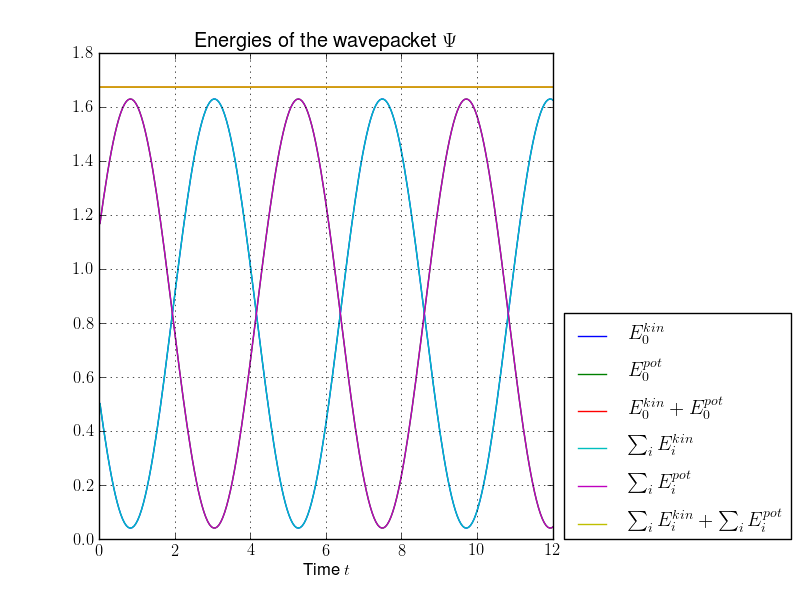
\includegraphics[width=0.5\linewidth]{./results/HO/energies_block0.png}
  }
  \subfloat[][]{
    \label{fig:ho_energy_drift}
    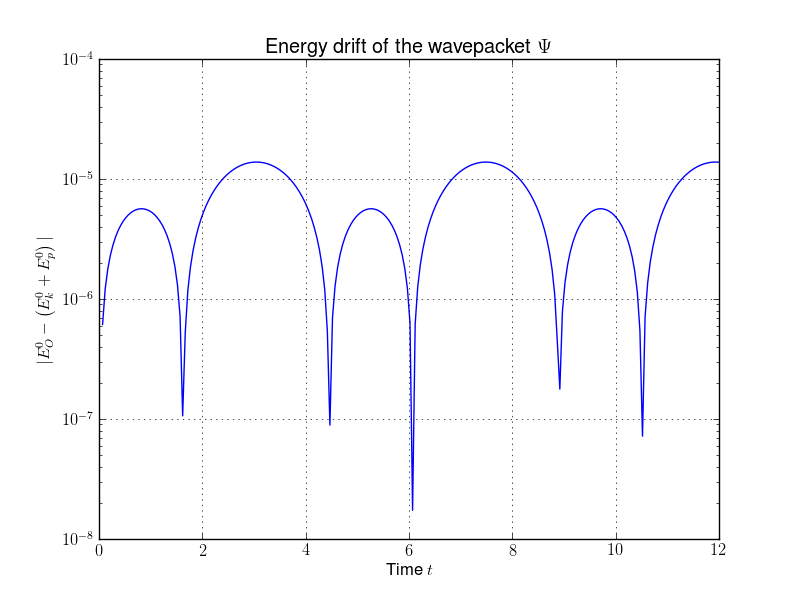
\includegraphics[width=0.5\linewidth]{./results/HO/energy_drift_block0_log.png}
  } \\
  \caption[Energies of a wavepacket in an harmonic oscillator]
          {The kinetic, potential and total energy and the drift of the
           total energy of a wavepacket in a two-dimensional harmonic oscillator.
    \subref{fig:ho_energies} The energies.
    \subref{fig:ho_energy_drift} The energy drift.
    \label{fig:ho_energy_plots}
  }
\end{figure}

\begin{figure}
  \centering
  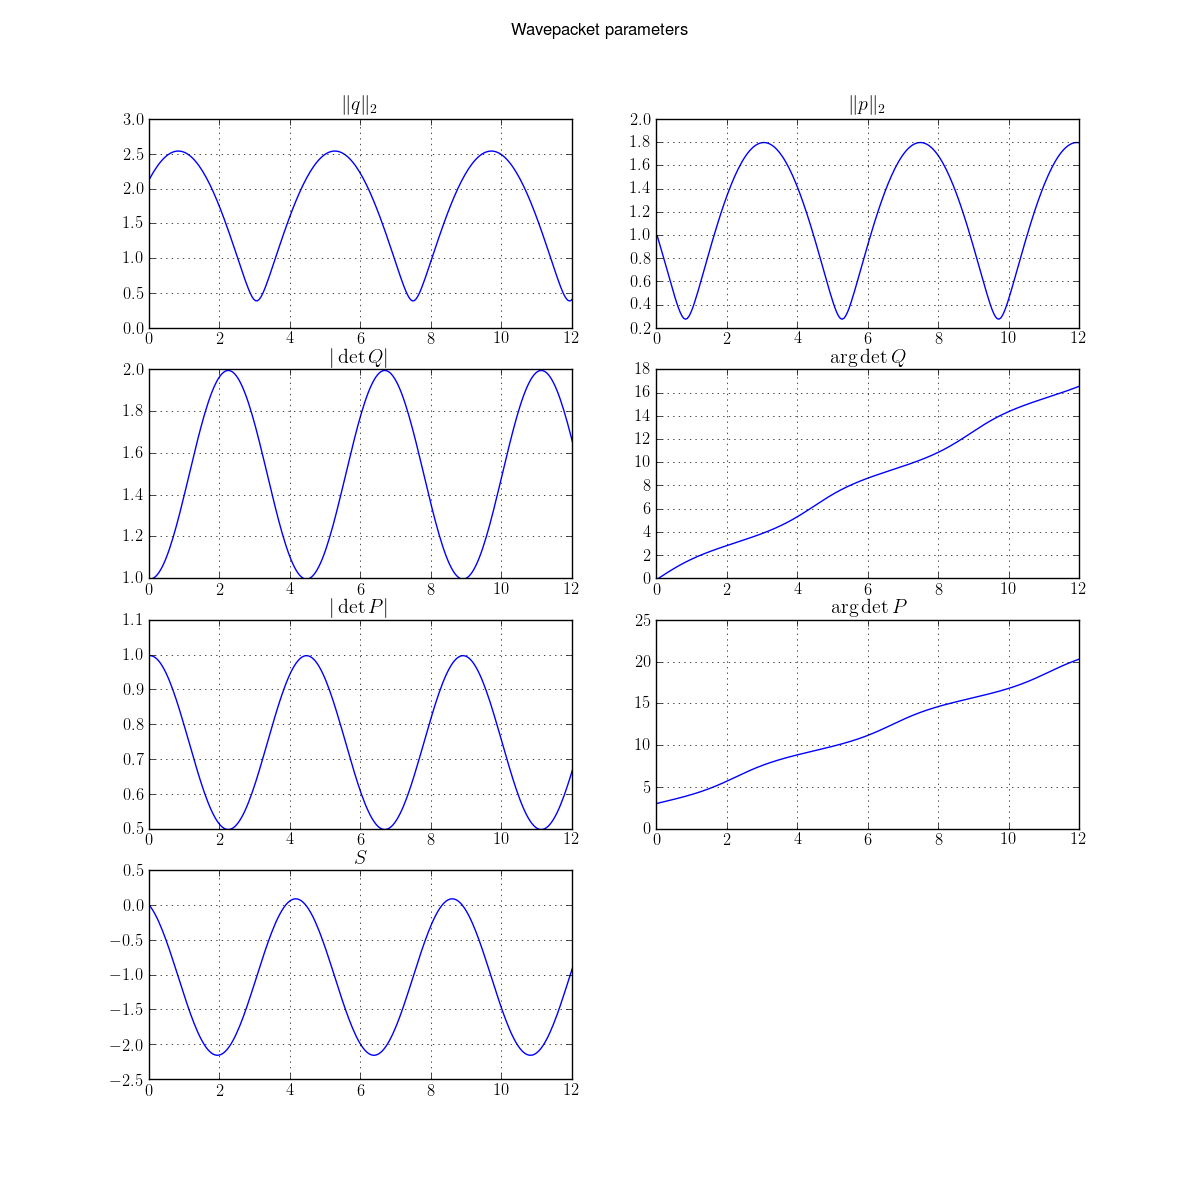
\includegraphics[width=\linewidth]{./results/HO/wavepacket_parameters_abs_ang_block0.png}
  \caption{Time-evolution of the parameter set $\Pi$ of a wavepacket in a
           two-dimensional harmonic oscillator.}
  \label{fig:ho_parameters}
\end{figure}

\begin{figure}
  \centering
  \subfloat[][]{
    \label{fig:ho_traject_q}
    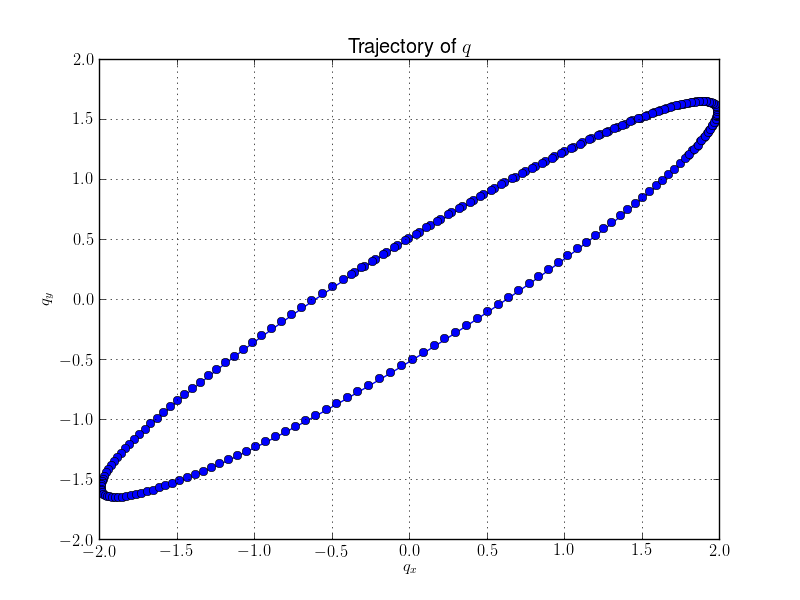
\includegraphics[width=0.5\linewidth]{./results/HO/wavepacket_parameters_trajectoryq_block0.png}
  }
  \subfloat[][]{
    \label{fig:ho_traject_p}
    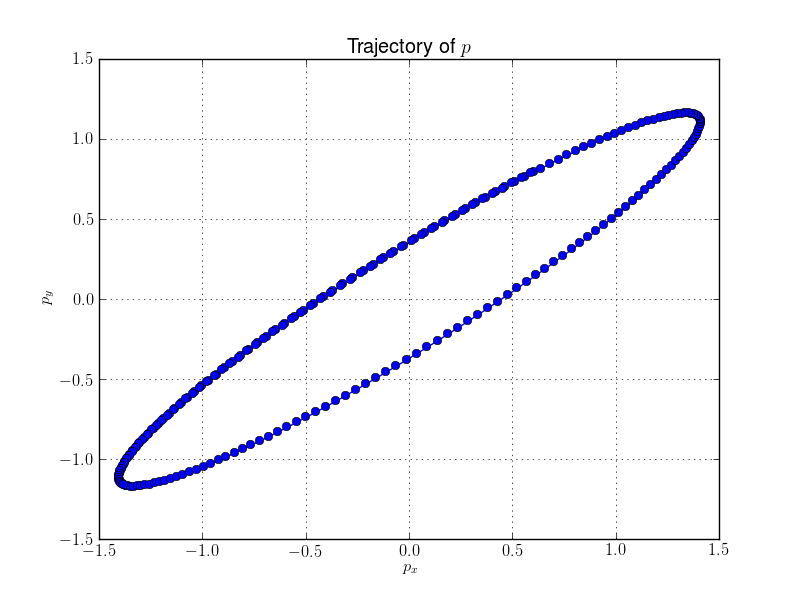
\includegraphics[width=0.5\linewidth]{./results/HO/wavepacket_parameters_trajectoryp_block0.png}
  } \\
  \caption[Trajectories of the position and momentum parameters]{
    Trajectories of the parameters $\vec{q}$ and $\vec{p}$.
    \subref{fig:ho_traject_q} Trajectory of $\vec{q}$.
    \subref{fig:ho_traject_p} Trajectory of $\vec{p}$.
    \label{fig:ho_traject_qp}
  }
\end{figure}

\begin{figure}
  \centering
  \subfloat[][]{
    \label{fig:ho_traject_Q}
    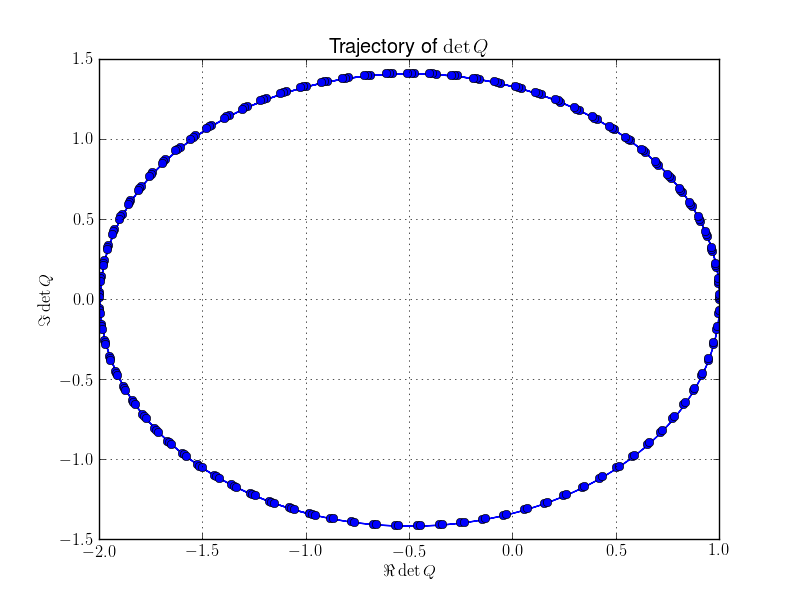
\includegraphics[width=0.5\linewidth]{./results/HO/wavepacket_parameters_trajectoryQ_block0.png}
  }
  \subfloat[][]{
    \label{fig:ho_traject_P}
    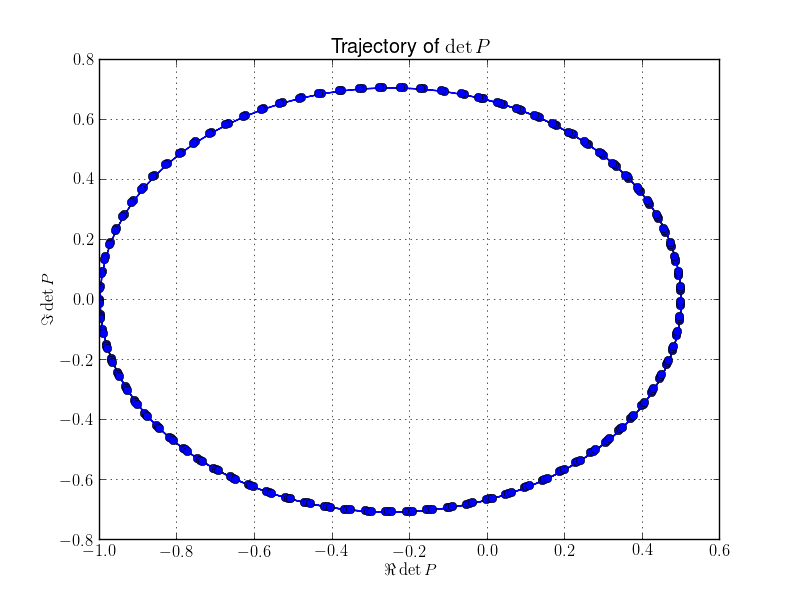
\includegraphics[width=0.5\linewidth]{./results/HO/wavepacket_parameters_trajectoryP_block0.png}
  } \\
  \caption[Trajectories of the spread matrices]{
    Trajectories of $\det\mat{Q}$ and $\det\mat{P}$ in the complex plane.
    \subref{fig:ho_traject_Q} Trajectory of $\det\mat{Q}$.
    \subref{fig:ho_traject_P} Trajectory of $\det\mat{P}$.
    \label{fig:ho_traject_QP}
  }
\end{figure}

Another trivial but nice example is the combination of a free particle potential
with a harmonic oscillator. The potential is constant along one direction while
quadratic along the other, we get:

\begin{equation} \label{eq:harmonic_channel}
  V(x,y) \assign \frac{1}{4} y^2 \,.
\end{equation}

The following simulation results were obtained by starting with a Gaussian $\phi_0$
with parameters:

\begin{align*}
  \vec{q} = \begin{pmatrix}
              0 \\ 1
            \end{pmatrix}
  \quad
  \vec{p} = \begin{pmatrix}
              0 \\ 0
            \end{pmatrix}
  \quad
  \mat{Q} = \begin{pmatrix}
              1 & 0 \\ 0 & 1
            \end{pmatrix}
  \quad
  \mat{P} = \begin{pmatrix}
              i & 0 \\ 0 & i
            \end{pmatrix}
  \quad
  S = 0
\end{align*}

and $\varepsilon = 0.1$.

\begin{figure}
  \centering
  \subfloat[][]{
    \label{fig:hofp_energies}
    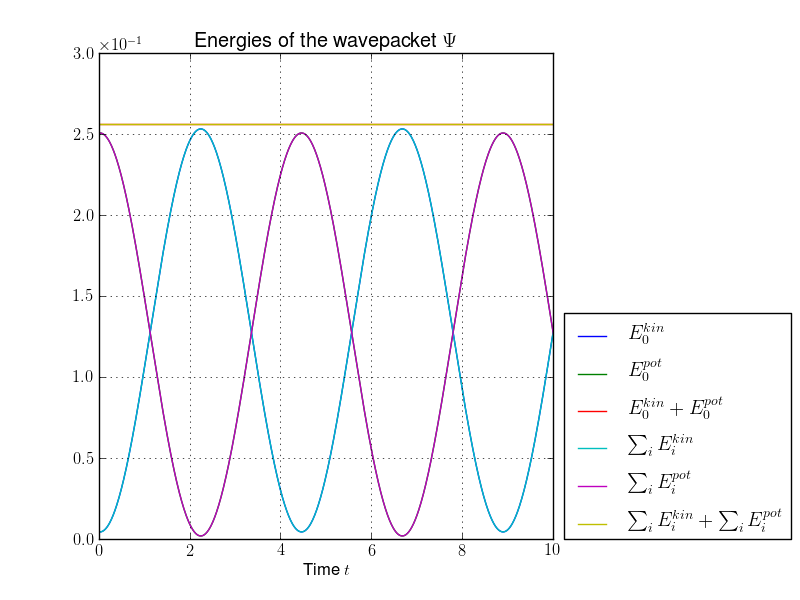
\includegraphics[width=0.5\linewidth]{./results/HO_FP/energies_block0.png}
  }
  \subfloat[][]{
    \label{fig:hofp_energy_drift}
    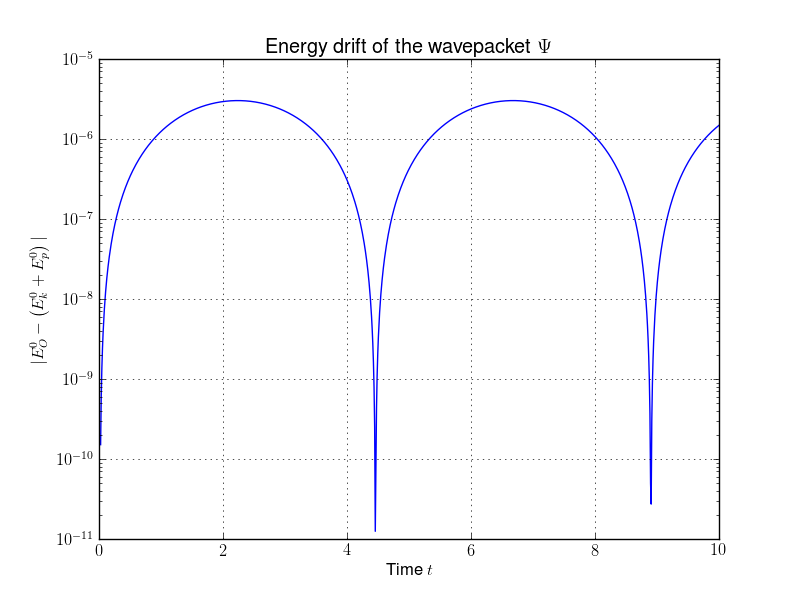
\includegraphics[width=0.5\linewidth]{./results/HO_FP/energy_drift_block0_log.png}
  } \\
  \caption[Energies of a wavepacket in a channel like oscillator]
          {The kinetic, potential and total energy and the drift of the
           total energy of a Gaussian wavepacket in the potential in \eqref{eq:harmonic_channel}.
    \subref{fig:hofp_energies} The energies.
    \subref{fig:hofp_energy_drift} The energy drift.
    \label{fig:hofp_energy_plots}
  }
\end{figure}

\begin{figure}
  \centering
  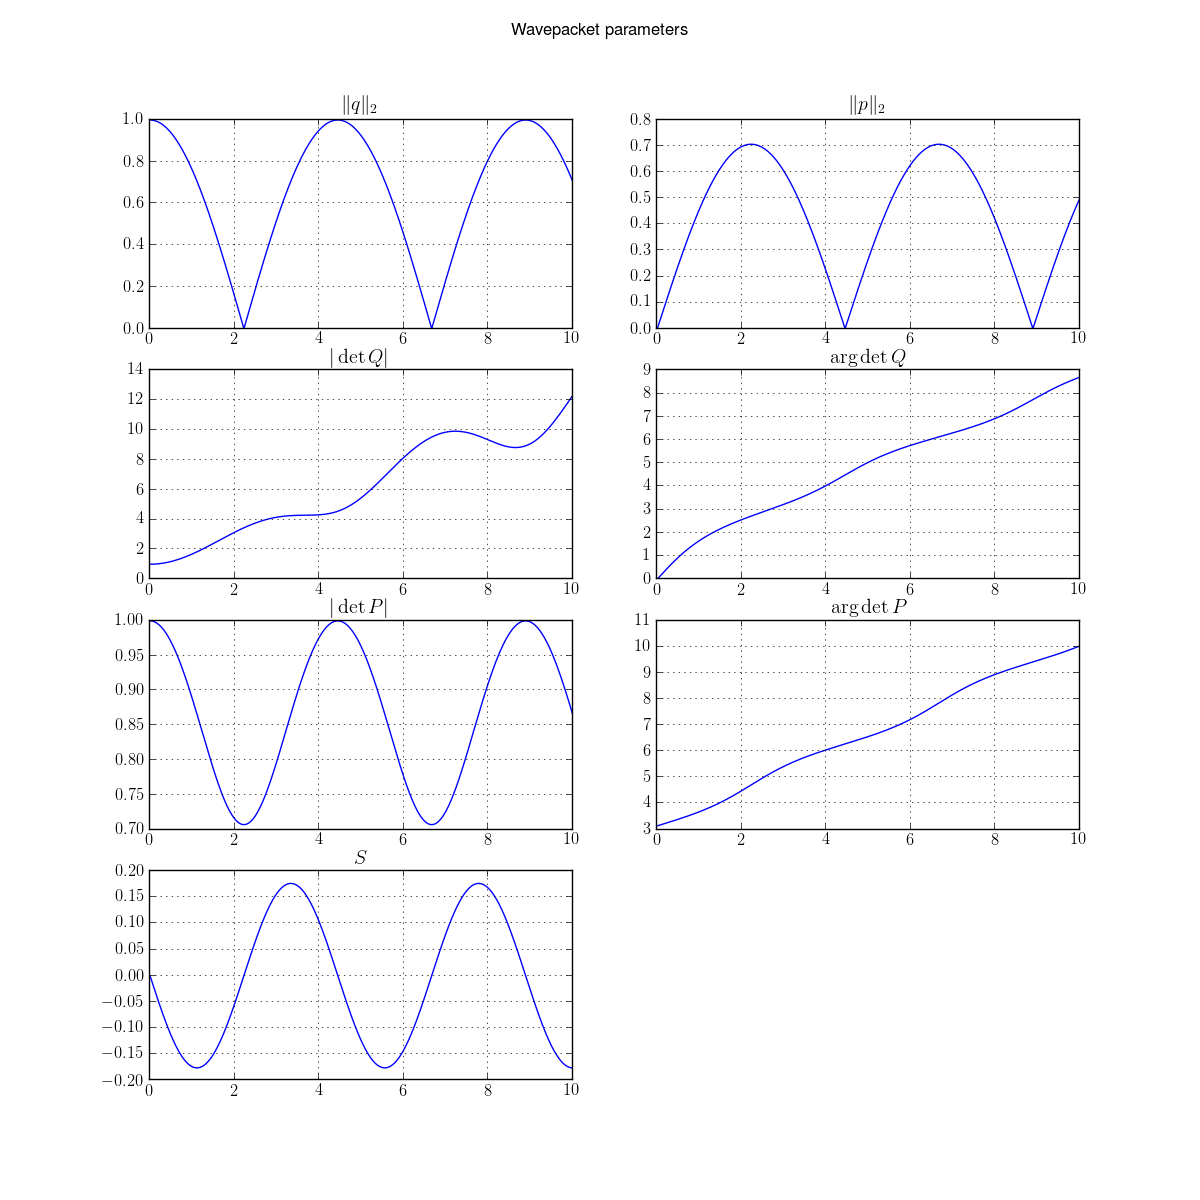
\includegraphics[width=\linewidth]{./results/HO_FP/wavepacket_parameters_abs_ang_block0.png}
  \caption{Time-evolution of the parameter set $\Pi$ of a Gaussian wavepacket in
           the potential in \eqref{eq:harmonic_channel}.}
  \label{fig:hofp_parameters}
\end{figure}

\begin{figure}
  \centering
  \subfloat[][]{
    \label{fig:hofp_traject_Q}
    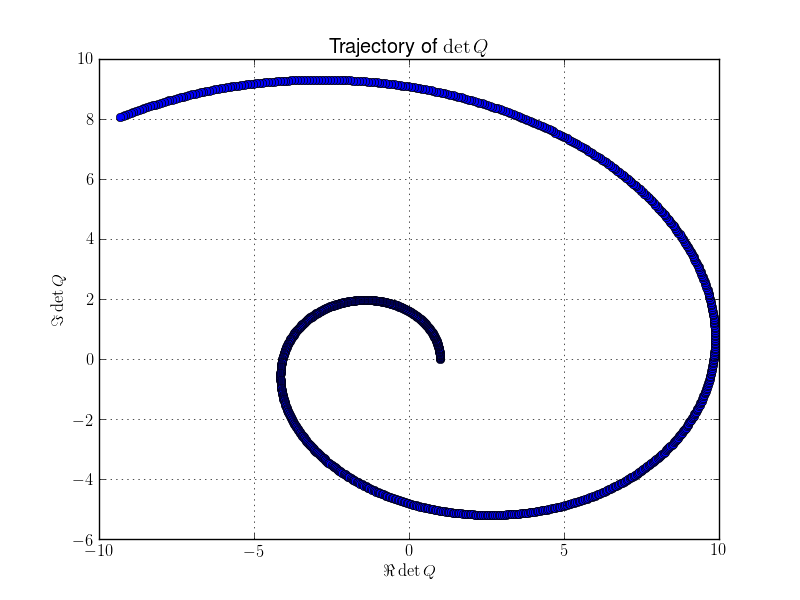
\includegraphics[width=0.5\linewidth]{./results/HO_FP/wavepacket_parameters_trajectoryQ_block0.png}
  }
  \subfloat[][]{
    \label{fig:hofp_traject_P}
    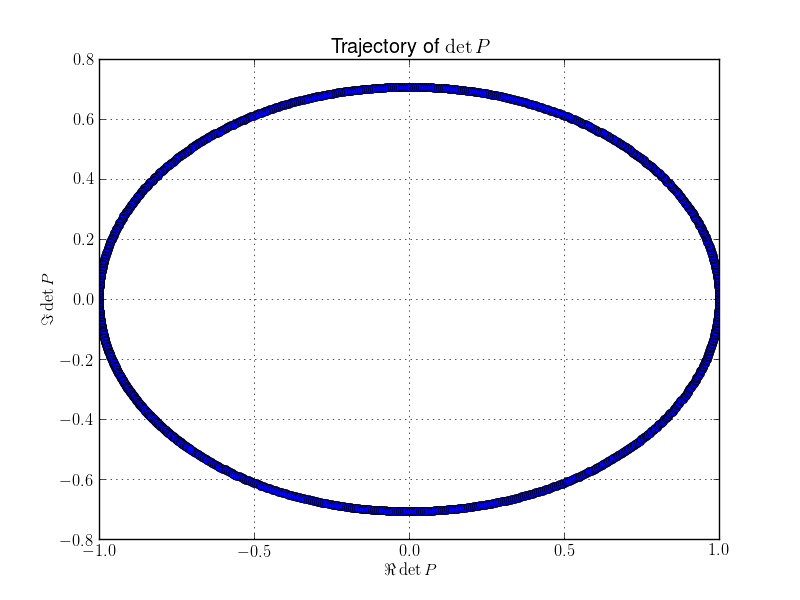
\includegraphics[width=0.5\linewidth]{./results/HO_FP/wavepacket_parameters_trajectoryP_block0.png}
  } \\
  \caption[Trajectories of the spread matrices]{
    Trajectories of $\det\mat{Q}$ and $\det\mat{P}$ in the complex plane.
    \subref{fig:hofp_traject_Q} Trajectory of $\det\mat{Q}$.
    \subref{fig:hofp_traject_P} Trajectory of $\det\mat{P}$.
    \label{fig:hofp_traject_QP}
  }
\end{figure}

An interesting fact appears if we look at the two eigenvalues $\lambda_0$ and $\lambda_1$
of $\mat{Q}$. We see that one oscillates and the other grows ad infinitum. Figure
\ref{fig:hofp_ev_Q} shows plots of $\lambda_0(t)$ and $\lambda_1(t)$.

\begin{figure}
  \centering
  \subfloat[][]{
    \label{fig:hofp_ev_Q_reim}
    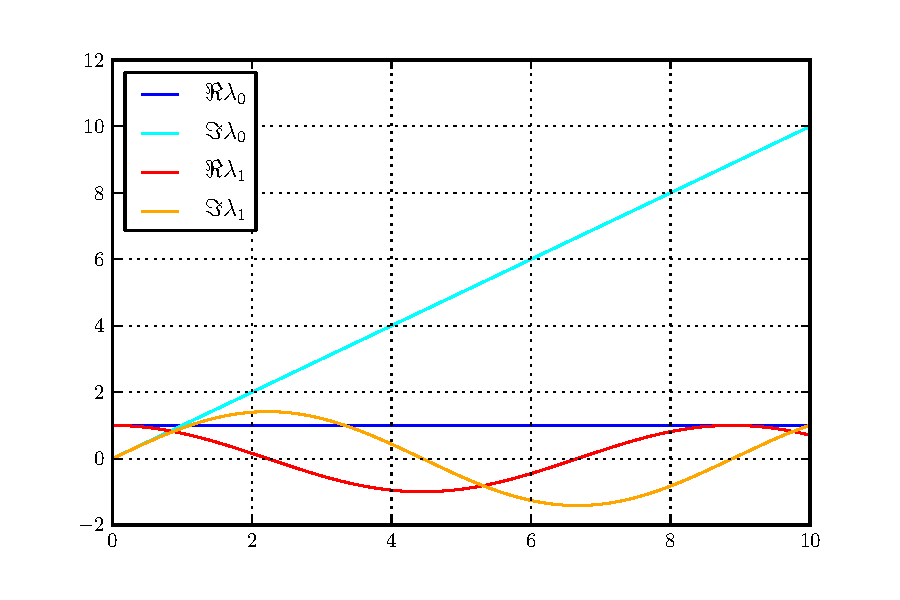
\includegraphics[width=0.5\linewidth]{./results/HO_FP/tube_reim_ev.pdf}
  }
  \subfloat[][]{
    \label{fig:hofp_ev_Q_abs}
    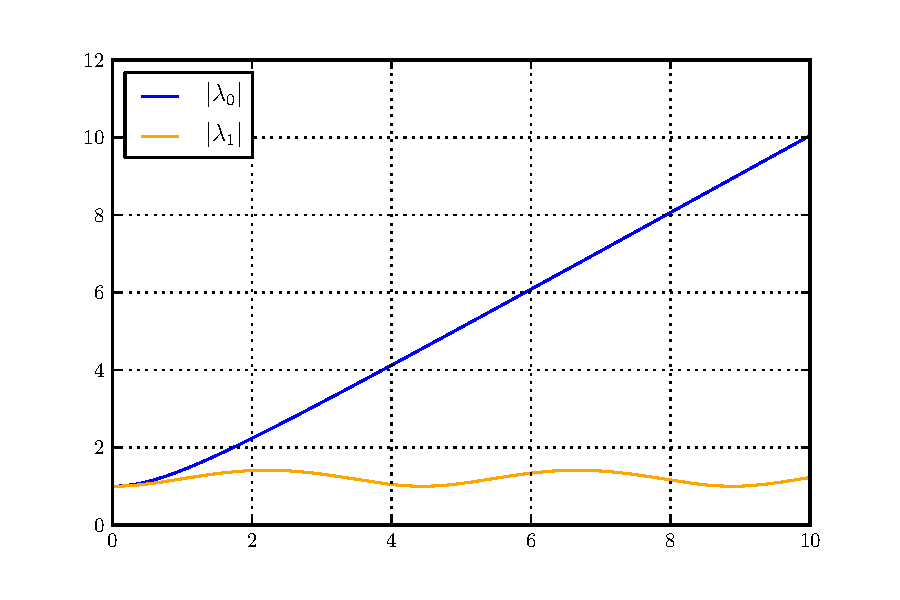
\includegraphics[width=0.5\linewidth]{./results/HO_FP/tube_abs_ev.pdf}
  } \\
  \caption[Eigenvalues of $Q$]{
    Time-evolution of the eigenvalues $\lambda_0$ and $\lambda_1$ of $\mat{Q}$.
    \subref{fig:hofp_ev_Q_reim} Real and imaginary parts.
    \subref{fig:hofp_ev_Q_abs} Absolute values.
    \label{fig:hofp_ev_Q}
  }
\end{figure}


\FloatBarrier
\section{Reproducing some other results}

We try to reproduce the results in section 5.1 of \cite{FGL_semiclassical_dynamics}.
The torsional potential in two dimensions is given by the expression:

\begin{equation}
  V(x,y) \assign (1-\cos(x)) + (1-\cos(y))
\end{equation}

and plotted in figure \ref{fig:torsional_potential}.

\begin{figure}
  \centering
  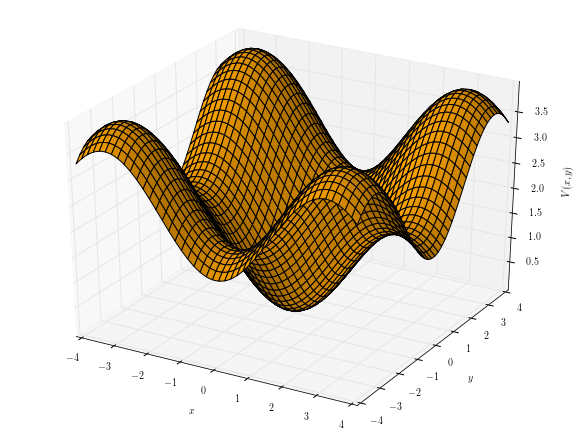
\includegraphics[scale=0.35]{./fig/torsional.png}
  \caption{The torsional potential in two dimensions.}
  \label{fig:torsional_potential}
\end{figure}

The initial parameter set $\Pi = \{\vec{q}, \vec{p}, \mat{Q}, \mat{P}, S\}$
for the wavepacket $\Psi = \phi_{0,0}$ is given as:

\begin{align*}
  \vec{q} = \begin{pmatrix}
              1 \\ 0
            \end{pmatrix}
  \quad
  \vec{p} = \begin{pmatrix}
              0 \\ 0
            \end{pmatrix}
  \quad
  \mat{Q} = \begin{pmatrix}
              1 & 0 \\ 0 & 1
            \end{pmatrix}
  \quad
  \mat{P} = \begin{pmatrix}
              i & 0 \\ 0 & i
            \end{pmatrix}
  \quad
  S = 0 \,.
\end{align*}

We use a hyperbolic cut basis shape $\mathfrak{K}$ with a cutoff value of $K=8$.
This yields 20 basis functions in total. For each simulation we use a time step
$\tau = 0.01$ and simulate until an end time of $T=20$. We perform three simulations
for different values of the semi-classical scaling parameter $\varepsilon$
\footnote{Note that we write $\varepsilon^2$ for what the authors of the paper call $\epsilon$.}.

\begin{figure}
  \centering
  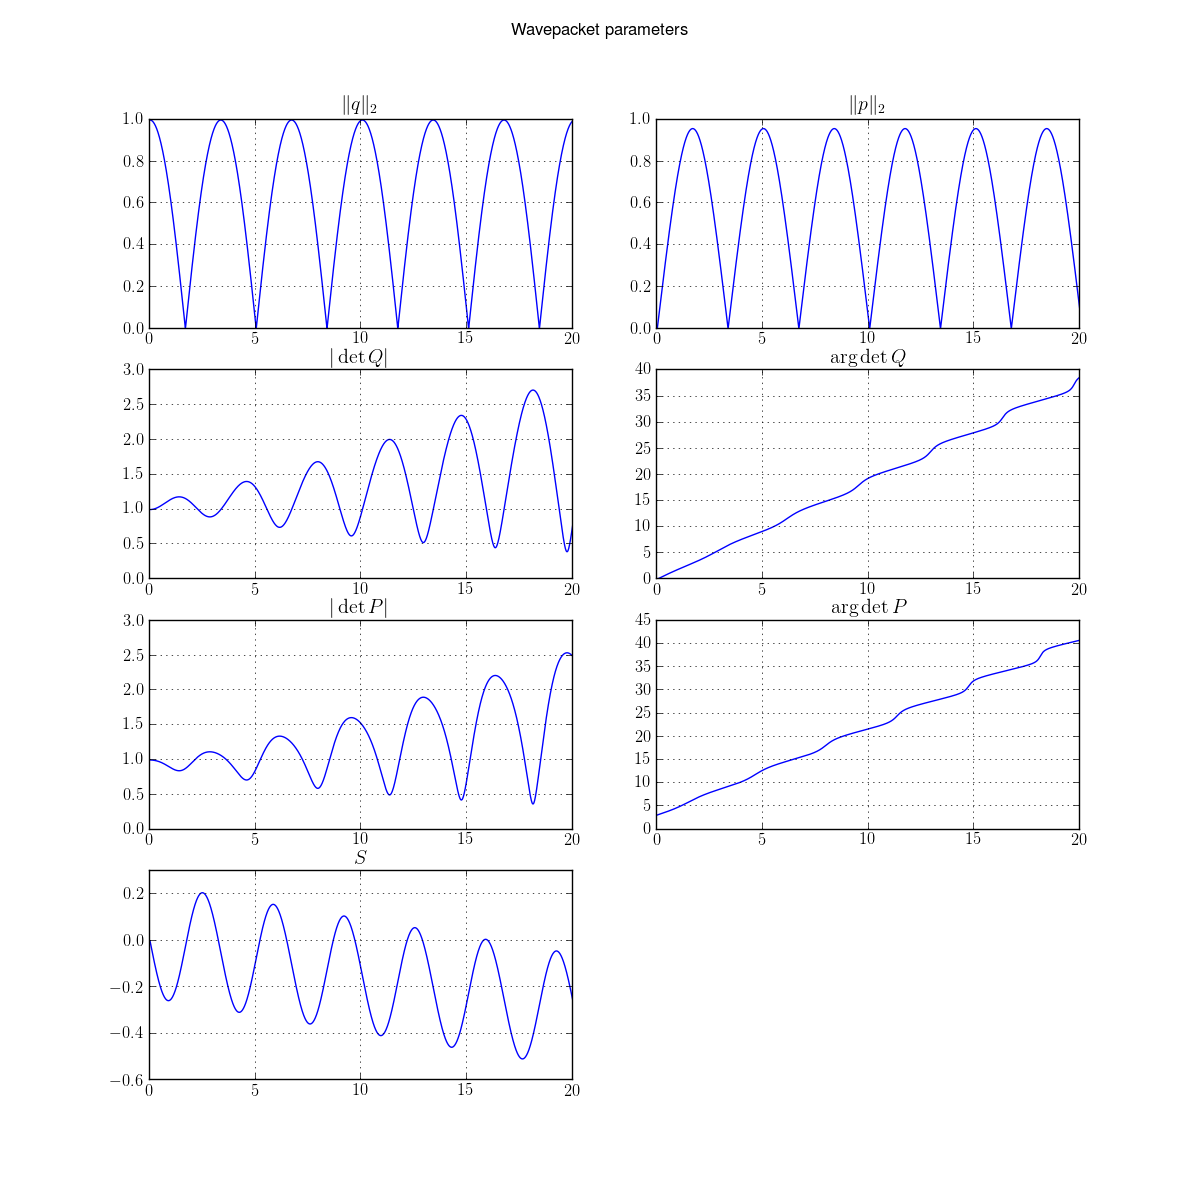
\includegraphics[width=\linewidth]{./results/config_cos_2_packets_case1/wavepacket_parameters_abs_ang_block0.png}
  \caption{Propagation of the parameter set $\Pi$. This is the same for all $\varepsilon$.}
  \label{fig:trosional_parameter_evolution}
\end{figure}

\begin{figure}
  \centering
  \subfloat[][]{
    \label{fig:torsional_case1_energies}
    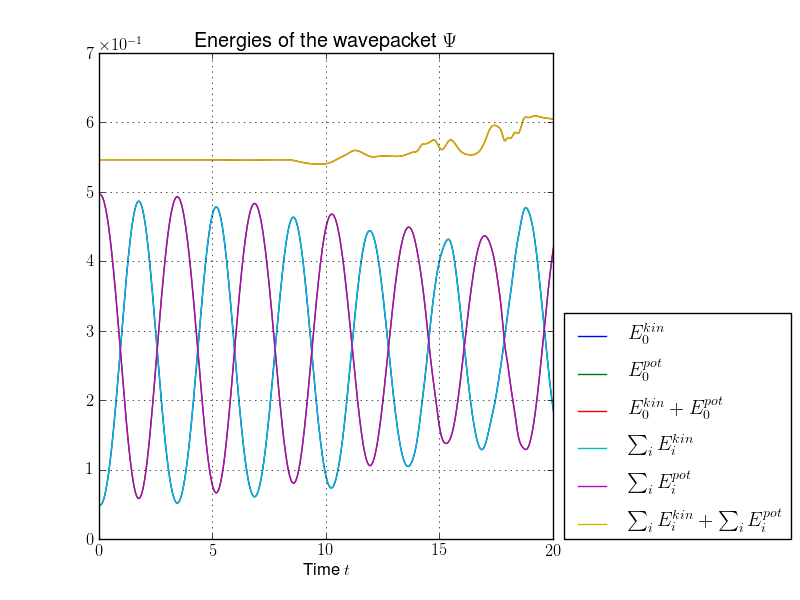
\includegraphics[width=0.5\linewidth]{./results/config_cos_2_packets_case1/energies_block0.png}
  }
  \subfloat[][]{
    \label{fig:torsional_case1_energy_drift}
    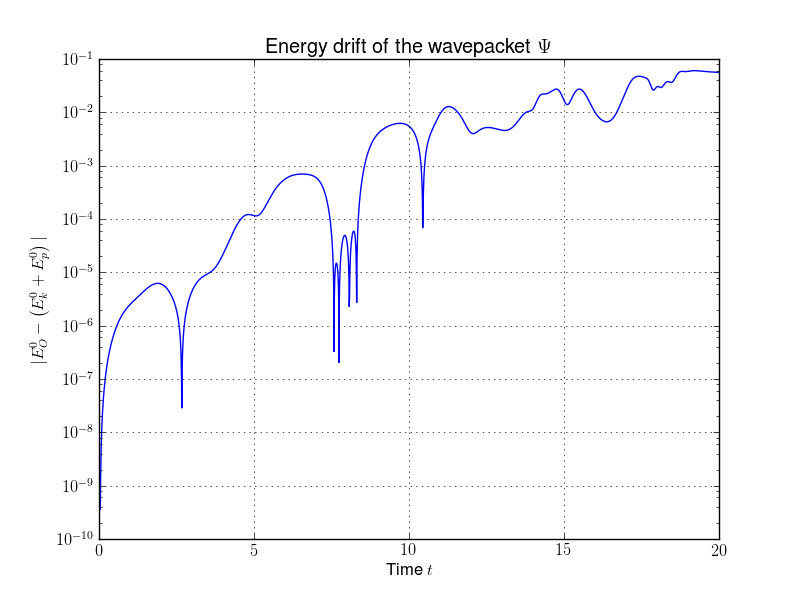
\includegraphics[width=0.5\linewidth]{./results/config_cos_2_packets_case1/energy_drift_block0_log.png}
  } \\
  \subfloat[][]{
    \label{fig:torsional_case2_energies}
    \includegraphics[width=0.5\linewidth]{./results/config_cos_2_packets_case2/energies_block0.png}
  }
  \subfloat[][]{
    \label{fig:torsional_case2_energy_drift}
    \includegraphics[width=0.5\linewidth]{./results/config_cos_2_packets_case2/energy_drift_block0_log.png}
  } \\
  \subfloat[][]{
    \label{fig:torsional_case3_energies}
    \includegraphics[width=0.5\linewidth]{./results/config_cos_2_packets_case3/energies_block0.png}
  }
  \subfloat[][]{
    \label{fig:torsional_case3_energy_drift}
    \includegraphics[width=0.5\linewidth]{./results/config_cos_2_packets_case3/energy_drift_block0_log.png}
  } \\
  \caption[Plots of the energies and drifts of a Gaussian in a torsional potential]{
    Plots of the kinetic, potential and total energy and the drift of the total energy
    of a Gaussian wavepacket in a 2D torsional potential. Note that despite of some violation of
    the total energy conservation we obtained perfect norm conservation (not shown here).
    A larger basis set would reduce the error.
    \subref{fig:torsional_case1_energies}, \subref{fig:torsional_case1_energy_drift}
    A wavepacket $\Ket{\Psi} = \phi_{0,0}$ with $\varepsilon = \sqrt{0.1}$.
    \subref{fig:torsional_case2_energies}, \subref{fig:torsional_case2_energy_drift}
    A wavepacket $\Ket{\Psi} = \phi_{0,0}$ with $\varepsilon = \sqrt{0.01}$.
    \subref{fig:torsional_case3_energies}, \subref{fig:torsional_case3_energy_drift}
    A wavepacket $\Ket{\Psi} = \phi_{0,0}$ with $\varepsilon = \sqrt{0.001}$.
%     \subref{fig:torsional_case1_energies} A wavepacket $\Ket{\Psi} = \phi_{0,0}$ with $\varepsilon = \sqrt{0.1}$.
%     \subref{fig:torsional_case1_energy_drift} A wavepacket $\Ket{\Psi} = \phi_{0,0}$ with $\varepsilon = \sqrt{0.1}$.
%     \subref{fig:torsional_case2_energies} A wavepacket $\Ket{\Psi} = \phi_{0,0}$ with $\varepsilon = \sqrt{0.01}$.
%     \subref{fig:torsional_case2_energy_drift} A wavepacket $\Ket{\Psi} = \phi_{0,0}$ with $\varepsilon = \sqrt{0.01}$.
%     \subref{fig:torsional_case3_energies} A wavepacket $\Ket{\Psi} = \phi_{0,0}$ with $\varepsilon = \sqrt{0.001}$.
%     \subref{fig:torsional_case3_energy_drift} A wavepacket $\Ket{\Psi} = \phi_{0,0}$ with $\varepsilon = \sqrt{0.001}$.
    \label{fig:torsional_energies}
  }
\end{figure}


\FloatBarrier
\section{A simple avoided crossing}

We generalise a model for a single avoided crossing of two energy levels.
The one-dimensional potential was studied in \cite{FGL_semiclassical_dynamics, B_bachelor_thesis}.
We extend this potential to two dimensions by making it rotationally symmetric. The equation
for $\mat{V}$ becomes:

\begin{equation} \label{eq:rotgap_avoided_crossing}
  \mat{V}(x,y) \assign
  \begin{pmatrix}
    \frac{1}{2} \tanh{\left(\sqrt{x^2 + y^2} \right)} & \delta \\
    \delta                                            & - \frac{1}{2} \tanh{\left(\sqrt{x^2 + y^2}\right)}
  \end{pmatrix}
\end{equation}

with $\delta$ being half of the energy level gap. The potential is shown in figure \ref{fig:rotgap_avoided_crossing}.

\begin{figure}[ht!]
  \centering
  \includegraphics[width=0.7\linewidth]{./fig/delta_gap_rotsym.png}
  \caption{Energy levels of the avoided crossing given by equation \eqref{eq:rotgap_avoided_crossing}
          for $\delta = 0.08$.}
  \label{fig:rotgap_avoided_crossing}
\end{figure}

In the following simulation results we varied the value of $\varepsilon$ and the gap size $\delta$.
The initial parameter values are:

\begin{align*}
  \vec{q} = \begin{pmatrix}
              -3 \\ 0
            \end{pmatrix}
  \quad
  \vec{p} = \begin{pmatrix}
              0.5 \\ 0
            \end{pmatrix}
  \quad
  \mat{Q} = \begin{pmatrix}
              1 & 0 \\ 0 & 1
            \end{pmatrix}
  \quad
  \mat{P} = \begin{pmatrix}
              i & 0 \\ 0 & i
            \end{pmatrix}
  \quad
  S = 0 \,.
\end{align*}

The timestep was set to $\tau = 0.01$.


\begin{figure}
  \centering
  \subfloat[][]{
    \label{fig:dgr_16_0-01_0-01_e}
    \includegraphics[width=0.5\linewidth]{./results/deltagap_rotsym/Parameters[bsize=16][eps=0-01][delta=0-01]/energies_block0.png}
  }
  \subfloat[][]{
    \label{fig:dgr_16_0-01_0-01_ed}
    \includegraphics[width=0.5\linewidth]{./results/deltagap_rotsym/Parameters[bsize=16][eps=0-01][delta=0-01]/energy_drift_block0_log.png}
  } \\
  \subfloat[][]{
    \label{fig:dgr_16_0-01_0-05_e}
    \includegraphics[width=0.5\linewidth]{./results/deltagap_rotsym/Parameters[bsize=16][eps=0-01][delta=0-05]/energies_block0.png}
  }
  \subfloat[][]{
    \label{fig:dgr_16_0-01_0-05_ed}
    \includegraphics[width=0.5\linewidth]{./results/deltagap_rotsym/Parameters[bsize=16][eps=0-01][delta=0-05]/energy_drift_block0_log.png}
  } \\
  \subfloat[][]{
    \label{fig:dgr_16_0-01_0-1_e}
    \includegraphics[width=0.5\linewidth]{./results/deltagap_rotsym/Parameters[bsize=16][eps=0-01][delta=0-1]/energies_block0.png}
  }
  \subfloat[][]{
    \label{fig:dgr_16_0-01_0-1_ed}
    \includegraphics[width=0.5\linewidth]{./results/deltagap_rotsym/Parameters[bsize=16][eps=0-01][delta=0-1]/energy_drift_block0_log.png}
  } \\
  \caption[Plots of the energies and drifts for a simple avoided crossing]{
    Plots of the kinetic, potential and total energy and the drift of the total energy
    of a Gaussian wavepacket $\Ket{\Psi} = \phi_{0,0}$. The basis shape is a hyperbolic cut with cut-off $K = 16$
    and $\varepsilon = 0.01$. The simulations for $\delta = 0.01$ would need a larger
    basis to work properly.
    \subref{fig:dgr_16_0-01_0-01_e}, \subref{fig:dgr_16_0-01_0-01_ed} $\delta = 0.01$
    \subref{fig:dgr_16_0-01_0-05_e}, \subref{fig:dgr_16_0-01_0-05_ed} $\delta = 0.05$
    \subref{fig:dgr_16_0-01_0-1_e}, \subref{fig:dgr_16_0-01_0-1_ed} $\delta = 0.1$
%     \subref{fig:dgr_16_0-01_0-01_e} $\delta = 0.01$
%     \subref{fig:dgr_16_0-01_0-01_ed} $\delta = 0.01$
%     \subref{fig:dgr_16_0-01_0-05_e} $\delta = 0.05$
%     \subref{fig:dgr_16_0-01_0-05_ed} $\delta = 0.05$
%     \subref{fig:dgr_16_0-01_0-1_e} $\delta = 0.1$
%     \subref{fig:dgr_16_0-01_0-1_ed} $\delta = 0.1$
    \label{fig:deltagap_rotsym_16_energies_eps_001_part1}
  }
\end{figure}


\begin{figure}
  \centering
  \subfloat[][]{
    \label{fig:dgr_16_0-01_0-2_e}
    \includegraphics[width=0.5\linewidth]{./results/deltagap_rotsym/Parameters[bsize=16][eps=0-01][delta=0-2]/energies_block0.png}
  }
  \subfloat[][]{
    \label{fig:dgr_16_0-01_0-2_ed}
    \includegraphics[width=0.5\linewidth]{./results/deltagap_rotsym/Parameters[bsize=16][eps=0-01][delta=0-2]/energy_drift_block0_log.png}
  } \\
  \subfloat[][]{
    \label{fig:dgr_16_0-01_0-5_e}
    \includegraphics[width=0.5\linewidth]{./results/deltagap_rotsym/Parameters[bsize=16][eps=0-01][delta=0-5]/energies_block0.png}
  }
  \subfloat[][]{
    \label{fig:dgr_16_0-01_0-5_ed}
    \includegraphics[width=0.5\linewidth]{./results/deltagap_rotsym/Parameters[bsize=16][eps=0-01][delta=0-5]/energy_drift_block0_log.png}
  } \\
  \subfloat[][]{
    \label{fig:dgr_16_0-01_1-0_e}
    \includegraphics[width=0.5\linewidth]{./results/deltagap_rotsym/Parameters[bsize=16][eps=0-01][delta=1-0]/energies_block0.png}
  }
  \subfloat[][]{
    \label{fig:dgr_16_0-01_1-0_ed}
    \includegraphics[width=0.5\linewidth]{./results/deltagap_rotsym/Parameters[bsize=16][eps=0-01][delta=1-0]/energy_drift_block0_log.png}
  } \\
  \caption[Plots of the energies and drifts for a simple avoided crossing]{
    Plots of the kinetic, potential and total energy and the drift of the total energy
    of a Gaussian wavepacket $\Ket{\Psi} = \phi_{0,0}$. The basis shape is a hyperbolic cut with cut-off $K = 16$
    and $\varepsilon = 0.01$.
    \subref{fig:dgr_16_0-01_0-2_e}, \subref{fig:dgr_16_0-01_0-2_ed} $\delta = 0.2$
    \subref{fig:dgr_16_0-01_0-5_e}, \subref{fig:dgr_16_0-01_0-5_ed} $\delta = 0.5$
    \subref{fig:dgr_16_0-01_1-0_e}, \subref{fig:dgr_16_0-01_1-0_ed} $\delta = 1.0$
%     \subref{fig:dgr_16_0-01_0-2_e} $\delta = 0.2$
%     \subref{fig:dgr_16_0-01_0-2_ed} $\delta = 0.2$
%     \subref{fig:dgr_16_0-01_0-5_e} $\delta = 0.5$
%     \subref{fig:dgr_16_0-01_0-5_ed} $\delta = 0.5$
%     \subref{fig:dgr_16_0-01_1-0_e} $\delta = 1.0$
%     \subref{fig:dgr_16_0-01_1-0_ed} $\delta = 1.0$
    \label{fig:deltagap_rotsym_16_energies_eps_001_part2}
  }
\end{figure}


\begin{figure}
  \centering
  \subfloat[][]{
    \label{fig:dgr_16_0-01_0-01_n}
    \includegraphics[width=0.5\linewidth]{./results/deltagap_rotsym/Parameters[bsize=16][eps=0-01][delta=0-01]/norms_block0.png}
  }
  \subfloat[][]{
    \label{fig:dgr_16_0-01_0-01_nd}
    \includegraphics[width=0.5\linewidth]{./results/deltagap_rotsym/Parameters[bsize=16][eps=0-01][delta=0-01]/norms_drift_block0_log.png}
  } \\
  \subfloat[][]{
    \label{fig:dgr_16_0-01_0-05_n}
    \includegraphics[width=0.5\linewidth]{./results/deltagap_rotsym/Parameters[bsize=16][eps=0-01][delta=0-05]/norms_block0.png}
  }
  \subfloat[][]{
    \label{fig:dgr_16_0-01_0-05_nd}
    \includegraphics[width=0.5\linewidth]{./results/deltagap_rotsym/Parameters[bsize=16][eps=0-01][delta=0-05]/norms_drift_block0_log.png}
  } \\
  \subfloat[][]{
    \label{fig:dgr_16_0-01_0-1_n}
    \includegraphics[width=0.5\linewidth]{./results/deltagap_rotsym/Parameters[bsize=16][eps=0-01][delta=0-1]/norms_block0.png}
  }
  \subfloat[][]{
    \label{fig:dgr_16_0-01_0-1_nd}
    \includegraphics[width=0.5\linewidth]{./results/deltagap_rotsym/Parameters[bsize=16][eps=0-01][delta=0-1]/norms_drift_block0_log.png}
  } \\
  \caption[Plots of the norms and drifts for a simple avoided crossing]{
    Plots of the norm of the components on the upper and lower level and the drift of the total norm
    of a Gaussian wavepacket $\Ket{\Psi} = \phi_{0,0}$. The basis shape is a hyperbolic cut with cut-off $K = 16$
    and $\varepsilon = 0.01$.
    \subref{fig:dgr_16_0-01_0-01_n}, \subref{fig:dgr_16_0-01_0-01_nd} $\delta = 0.01$
    \subref{fig:dgr_16_0-01_0-05_n}, \subref{fig:dgr_16_0-01_0-05_nd} $\delta = 0.05$
    \subref{fig:dgr_16_0-01_0-1_n}, \subref{fig:dgr_16_0-01_0-1_nd} $\delta = 0.1$
%     \subref{fig:dgr_16_0-01_0-01_n} $\delta = 0.01$
%     \subref{fig:dgr_16_0-01_0-01_nd} $\delta = 0.01$
%     \subref{fig:dgr_16_0-01_0-05_n} $\delta = 0.05$
%     \subref{fig:dgr_16_0-01_0-05_nd} $\delta = 0.05$
%     \subref{fig:dgr_16_0-01_0-1_n} $\delta = 0.1$
%     \subref{fig:dgr_16_0-01_0-1_nd} $\delta = 0.1$
    \label{fig:deltagap_rotsym_16_norms_eps_001_part1}
  }
\end{figure}


\begin{figure}
  \centering
  \subfloat[][]{
    \label{fig:dgr_16_0-01_0-2_n}
    \includegraphics[width=0.5\linewidth]{./results/deltagap_rotsym/Parameters[bsize=16][eps=0-01][delta=0-2]/norms_block0.png}
  }
  \subfloat[][]{
    \label{fig:dgr_16_0-01_0-2_nd}
    \includegraphics[width=0.5\linewidth]{./results/deltagap_rotsym/Parameters[bsize=16][eps=0-01][delta=0-2]/norms_drift_block0_log.png}
  } \\
  \subfloat[][]{
    \label{fig:dgr_16_0-01_0-5_n}
    \includegraphics[width=0.5\linewidth]{./results/deltagap_rotsym/Parameters[bsize=16][eps=0-01][delta=0-5]/norms_block0.png}
  }
  \subfloat[][]{
    \label{fig:dgr_16_0-01_0-5_nd}
    \includegraphics[width=0.5\linewidth]{./results/deltagap_rotsym/Parameters[bsize=16][eps=0-01][delta=0-5]/norms_drift_block0_log.png}
  } \\
  \subfloat[][]{
    \label{fig:dgr_16_0-01_1-0_n}
    \includegraphics[width=0.5\linewidth]{./results/deltagap_rotsym/Parameters[bsize=16][eps=0-01][delta=1-0]/norms_block0.png}
  }
  \subfloat[][]{
    \label{fig:dgr_16_0-01_1-0_nd}
    \includegraphics[width=0.5\linewidth]{./results/deltagap_rotsym/Parameters[bsize=16][eps=0-01][delta=1-0]/norms_drift_block0_log.png}
  } \\
  \caption[Plots of the norms and drifts for a simple avoided crossing]{
    Plots of the norm of the components on the upper and lower level and the drift of the total norm
    of a Gaussian wavepacket $\Ket{\Psi} = \phi_{0,0}$. The basis shape is a hyperbolic cut with cut-off $K = 16$
    and $\varepsilon = 0.01$.
    \subref{fig:dgr_16_0-01_0-2_n}, \subref{fig:dgr_16_0-01_0-2_nd} $\delta = 0.2$
    \subref{fig:dgr_16_0-01_0-5_n}, \subref{fig:dgr_16_0-01_0-5_nd} $\delta = 0.5$
    \subref{fig:dgr_16_0-01_1-0_n}, \subref{fig:dgr_16_0-01_1-0_nd} $\delta = 1.0$
%     \subref{fig:dgr_16_0-01_0-2_n} $\delta = 0.2$
%     \subref{fig:dgr_16_0-01_0-2_nd} $\delta = 0.2$
%     \subref{fig:dgr_16_0-01_0-5_n} $\delta = 0.5$
%     \subref{fig:dgr_16_0-01_0-5_nd} $\delta = 0.5$
%     \subref{fig:dgr_16_0-01_1-0_n} $\delta = 1.0$
%     \subref{fig:dgr_16_0-01_1-0_nd} $\delta = 1.0$
    \label{fig:deltagap_rotsym_16_norms_eps_001_part2}
  }
\end{figure}


\begin{figure}
  \centering
  \subfloat[][]{
    \label{fig:dgr_16_0-05_0-01_e}
    \includegraphics[width=0.5\linewidth]{./results/deltagap_rotsym/Parameters[bsize=16][eps=0-05][delta=0-01]/energies_block0.png}
  }
  \subfloat[][]{
    \label{fig:dgr_16_0-05_0-01_ed}
    \includegraphics[width=0.5\linewidth]{./results/deltagap_rotsym/Parameters[bsize=16][eps=0-05][delta=0-01]/energy_drift_block0_log.png}
  } \\
  \subfloat[][]{
    \label{fig:dgr_16_0-05_0-05_e}
    \includegraphics[width=0.5\linewidth]{./results/deltagap_rotsym/Parameters[bsize=16][eps=0-05][delta=0-05]/energies_block0.png}
  }
  \subfloat[][]{
    \label{fig:dgr_16_0-05_0-05_ed}
    \includegraphics[width=0.5\linewidth]{./results/deltagap_rotsym/Parameters[bsize=16][eps=0-05][delta=0-05]/energy_drift_block0_log.png}
  } \\
  \subfloat[][]{
    \label{fig:dgr_16_0-05_0-1_e}
    \includegraphics[width=0.5\linewidth]{./results/deltagap_rotsym/Parameters[bsize=16][eps=0-05][delta=0-1]/energies_block0.png}
  }
  \subfloat[][]{
    \label{fig:dgr_16_0-05_0-1_ed}
    \includegraphics[width=0.5\linewidth]{./results/deltagap_rotsym/Parameters[bsize=16][eps=0-05][delta=0-1]/energy_drift_block0_log.png}
  } \\
  \caption[Plots of the energies and drifts for a simple avoided crossing]{
    Plots of the kinetic, potential and total energy and the drift of the total energy
    of a Gaussian wavepacket $\Ket{\Psi} = \phi_{0,0}$. The basis shape is a hyperbolic cut with cut-off $K = 16$
    and $\varepsilon = 0.05$.
    \subref{fig:dgr_16_0-05_0-01_e}, \subref{fig:dgr_16_0-05_0-01_ed} $\delta = 0.01$
    \subref{fig:dgr_16_0-05_0-05_e}, \subref{fig:dgr_16_0-05_0-05_ed} $\delta = 0.05$
    \subref{fig:dgr_16_0-05_0-1_e}, \subref{fig:dgr_16_0-05_0-1_ed} $\delta = 0.1$
%     \subref{fig:dgr_16_0-05_0-01_e} $\delta = 0.01$
%     \subref{fig:dgr_16_0-05_0-01_ed} $\delta = 0.01$
%     \subref{fig:dgr_16_0-05_0-05_e} $\delta = 0.05$
%     \subref{fig:dgr_16_0-05_0-05_ed} $\delta = 0.05$
%     \subref{fig:dgr_16_0-05_0-1_e} $\delta = 0.1$
%     \subref{fig:dgr_16_0-05_0-1_ed} $\delta = 0.1$
    \label{fig:deltagap_rotsym_16_energies_eps_005_part1}
  }
\end{figure}


\begin{figure}
  \centering
  \subfloat[][]{
    \label{fig:dgr_16_0-05_0-2_e}
    \includegraphics[width=0.5\linewidth]{./results/deltagap_rotsym/Parameters[bsize=16][eps=0-05][delta=0-2]/energies_block0.png}
  }
  \subfloat[][]{
    \label{fig:dgr_16_0-05_0-2_ed}
    \includegraphics[width=0.5\linewidth]{./results/deltagap_rotsym/Parameters[bsize=16][eps=0-05][delta=0-2]/energy_drift_block0_log.png}
  } \\
  \subfloat[][]{
    \label{fig:dgr_16_0-05_0-5_e}
    \includegraphics[width=0.5\linewidth]{./results/deltagap_rotsym/Parameters[bsize=16][eps=0-05][delta=0-5]/energies_block0.png}
  }
  \subfloat[][]{
    \label{fig:dgr_16_0-05_0-5_ed}
    \includegraphics[width=0.5\linewidth]{./results/deltagap_rotsym/Parameters[bsize=16][eps=0-05][delta=0-5]/energy_drift_block0_log.png}
  } \\
  \subfloat[][]{
    \label{fig:dgr_16_0-05_1-0_e}
    \includegraphics[width=0.5\linewidth]{./results/deltagap_rotsym/Parameters[bsize=16][eps=0-05][delta=1-0]/energies_block0.png}
  }
  \subfloat[][]{
    \label{fig:dgr_16_0-05_1-0_ed}
    \includegraphics[width=0.5\linewidth]{./results/deltagap_rotsym/Parameters[bsize=16][eps=0-05][delta=1-0]/energy_drift_block0_log.png}
  } \\
  \caption[Plots of the energies and drifts for a simple avoided crossing]{
    Plots of the kinetic, potential and total energy and the drift of the total energy
    of a Gaussian wavepacket $\Ket{\Psi} = \phi_{0,0}$. The basis shape is a hyperbolic cut with cut-off $K = 16$
    and $\varepsilon = 0.05$.
    \subref{fig:dgr_16_0-05_0-2_e}, \subref{fig:dgr_16_0-05_0-2_ed} $\delta = 0.2$
    \subref{fig:dgr_16_0-05_0-5_e}, \subref{fig:dgr_16_0-05_0-5_ed} $\delta = 0.5$
    \subref{fig:dgr_16_0-05_1-0_e}, \subref{fig:dgr_16_0-05_1-0_ed} $\delta = 1.0$
%     \subref{fig:dgr_16_0-05_0-2_e} $\delta = 0.2$
%     \subref{fig:dgr_16_0-05_0-2_ed} $\delta = 0.2$
%     \subref{fig:dgr_16_0-05_0-5_e} $\delta = 0.5$
%     \subref{fig:dgr_16_0-05_0-5_ed} $\delta = 0.5$
%     \subref{fig:dgr_16_0-05_1-0_e} $\delta = 1.0$
%     \subref{fig:dgr_16_0-05_1-0_ed} $\delta = 1.0$
    \label{fig:deltagap_rotsym_16_energies_eps_005_part2}
  }
\end{figure}


\begin{figure}
  \centering
  \subfloat[][]{
    \label{fig:dgr_16_0-05_0-01_n}
    \includegraphics[width=0.5\linewidth]{./results/deltagap_rotsym/Parameters[bsize=16][eps=0-05][delta=0-01]/norms_block0.png}
  }
  \subfloat[][]{
    \label{fig:dgr_16_0-05_0-01_nd}
    \includegraphics[width=0.5\linewidth]{./results/deltagap_rotsym/Parameters[bsize=16][eps=0-05][delta=0-01]/norms_drift_block0_log.png}
  } \\
  \subfloat[][]{
    \label{fig:dgr_16_0-05_0-05_n}
    \includegraphics[width=0.5\linewidth]{./results/deltagap_rotsym/Parameters[bsize=16][eps=0-05][delta=0-05]/norms_block0.png}
  }
  \subfloat[][]{
    \label{fig:dgr_16_0-05_0-05_nd}
    \includegraphics[width=0.5\linewidth]{./results/deltagap_rotsym/Parameters[bsize=16][eps=0-05][delta=0-05]/norms_drift_block0_log.png}
  } \\
  \subfloat[][]{
    \label{fig:dgr_16_0-05_0-1_n}
    \includegraphics[width=0.5\linewidth]{./results/deltagap_rotsym/Parameters[bsize=16][eps=0-05][delta=0-1]/norms_block0.png}
  }
  \subfloat[][]{
    \label{fig:dgr_16_0-05_0-1_nd}
    \includegraphics[width=0.5\linewidth]{./results/deltagap_rotsym/Parameters[bsize=16][eps=0-05][delta=0-1]/norms_drift_block0_log.png}
  } \\
  \caption[Plots of the norms and drifts for a simple avoided crossing]{
    Plots of the norm of the components on the upper and lower level and the drift of the total norm
    of a Gaussian wavepacket $\Ket{\Psi} = \phi_{0,0}$. The basis shape is a hyperbolic cut with cut-off $K = 16$
    and $\varepsilon = 0.05$.
    \subref{fig:dgr_16_0-05_0-01_n}, \subref{fig:dgr_16_0-05_0-01_nd} $\delta = 0.01$
    \subref{fig:dgr_16_0-05_0-05_n}, \subref{fig:dgr_16_0-05_0-05_nd} $\delta = 0.05$
    \subref{fig:dgr_16_0-05_0-1_n}, \subref{fig:dgr_16_0-05_0-1_nd} $\delta = 0.1$
%     \subref{fig:dgr_16_0-05_0-01_n} $\delta = 0.01$
%     \subref{fig:dgr_16_0-05_0-01_nd} $\delta = 0.01$
%     \subref{fig:dgr_16_0-05_0-05_n} $\delta = 0.05$
%     \subref{fig:dgr_16_0-05_0-05_nd} $\delta = 0.05$
%     \subref{fig:dgr_16_0-05_0-1_n} $\delta = 0.1$
%     \subref{fig:dgr_16_0-05_0-1_nd} $\delta = 0.1$
    \label{fig:deltagap_rotsym_16_norms_eps_005_part1}
  }
\end{figure}


\begin{figure}
  \centering
  \subfloat[][]{
    \label{fig:dgr_16_0-05_0-2_n}
    \includegraphics[width=0.5\linewidth]{./results/deltagap_rotsym/Parameters[bsize=16][eps=0-05][delta=0-2]/norms_block0.png}
  }
  \subfloat[][]{
    \label{fig:dgr_16_0-05_0-2_nd}
    \includegraphics[width=0.5\linewidth]{./results/deltagap_rotsym/Parameters[bsize=16][eps=0-05][delta=0-2]/norms_drift_block0_log.png}
  } \\
  \subfloat[][]{
    \label{fig:dgr_16_0-05_0-5_n}
    \includegraphics[width=0.5\linewidth]{./results/deltagap_rotsym/Parameters[bsize=16][eps=0-05][delta=0-5]/norms_block0.png}
  }
  \subfloat[][]{
    \label{fig:dgr_16_0-05_0-5_nd}
    \includegraphics[width=0.5\linewidth]{./results/deltagap_rotsym/Parameters[bsize=16][eps=0-05][delta=0-5]/norms_drift_block0_log.png}
  } \\
  \subfloat[][]{
    \label{fig:dgr_16_0-05_1-0_n}
    \includegraphics[width=0.5\linewidth]{./results/deltagap_rotsym/Parameters[bsize=16][eps=0-05][delta=1-0]/norms_block0.png}
  }
  \subfloat[][]{
    \label{fig:dgr_16_0-05_1-0_nd}
    \includegraphics[width=0.5\linewidth]{./results/deltagap_rotsym/Parameters[bsize=16][eps=0-05][delta=1-0]/norms_drift_block0_log.png}
  } \\
  \caption[Plots of the norms and drifts for a simple avoided crossing]{
    Plots of the norm of the components on the upper and lower level and the drift of the total norm
    of a Gaussian wavepacket $\Ket{\Psi} = \phi_{0,0}$. The basis shape is a hyperbolic cut with cut-off $K = 16$
    and $\varepsilon = 0.05$.
    \subref{fig:dgr_16_0-05_0-2_n}, \subref{fig:dgr_16_0-05_0-2_nd} $\delta = 0.2$
    \subref{fig:dgr_16_0-05_0-5_n}, \subref{fig:dgr_16_0-05_0-5_nd} $\delta = 0.5$
    \subref{fig:dgr_16_0-05_1-0_n}, \subref{fig:dgr_16_0-05_1-0_nd} $\delta = 1.0$
%     \subref{fig:dgr_16_0-05_0-2_n} $\delta = 0.2$
%     \subref{fig:dgr_16_0-05_0-2_nd} $\delta = 0.2$
%     \subref{fig:dgr_16_0-05_0-5_n} $\delta = 0.5$
%     \subref{fig:dgr_16_0-05_0-5_nd} $\delta = 0.5$
%     \subref{fig:dgr_16_0-05_1-0_n} $\delta = 1.0$
%     \subref{fig:dgr_16_0-05_1-0_nd} $\delta = 1.0$
    \label{fig:deltagap_rotsym_16_norms_eps_005_part2}
  }
\end{figure}


\begin{figure}
  \centering
  \subfloat[][]{
    \label{fig:dgr_16_0-1_0-01_e}
    \includegraphics[width=0.5\linewidth]{./results/deltagap_rotsym/Parameters[bsize=16][eps=0-1][delta=0-01]/energies_block0.png}
  }
  \subfloat[][]{
    \label{fig:dgr_16_0-1_0-01_ed}
    \includegraphics[width=0.5\linewidth]{./results/deltagap_rotsym/Parameters[bsize=16][eps=0-1][delta=0-01]/energy_drift_block0_log.png}
  } \\
  \subfloat[][]{
    \label{fig:dgr_16_0-1_0-05_e}
    \includegraphics[width=0.5\linewidth]{./results/deltagap_rotsym/Parameters[bsize=16][eps=0-1][delta=0-05]/energies_block0.png}
  }
  \subfloat[][]{
    \label{fig:dgr_16_0-1_0-05_ed}
    \includegraphics[width=0.5\linewidth]{./results/deltagap_rotsym/Parameters[bsize=16][eps=0-1][delta=0-05]/energy_drift_block0_log.png}
  } \\
  \subfloat[][]{
    \label{fig:dgr_16_0-1_0-1_e}
    \includegraphics[width=0.5\linewidth]{./results/deltagap_rotsym/Parameters[bsize=16][eps=0-1][delta=0-1]/energies_block0.png}
  }
  \subfloat[][]{
    \label{fig:dgr_16_0-1_0-1_ed}
    \includegraphics[width=0.5\linewidth]{./results/deltagap_rotsym/Parameters[bsize=16][eps=0-1][delta=0-1]/energy_drift_block0_log.png}
  } \\
  \caption[Plots of the energies and drifts for a simple avoided crossing]{
    Plots of the kinetic, potential and total energy and the drift of the total energy
    of a Gaussian wavepacket $\Ket{\Psi} = \phi_{0,0}$. The basis shape is a hyperbolic cut with cut-off $K = 16$
    and $\varepsilon = 0.1$.
    \subref{fig:dgr_16_0-1_0-01_e}, \subref{fig:dgr_16_0-1_0-01_ed} $\delta = 0.01$
    \subref{fig:dgr_16_0-1_0-05_e}, \subref{fig:dgr_16_0-1_0-05_ed} $\delta = 0.05$
    \subref{fig:dgr_16_0-1_0-1_e}, \subref{fig:dgr_16_0-1_0-1_ed} $\delta = 0.1$
%     \subref{fig:dgr_16_0-1_0-01_e} $\delta = 0.01$
%     \subref{fig:dgr_16_0-1_0-01_ed} $\delta = 0.01$
%     \subref{fig:dgr_16_0-1_0-05_e} $\delta = 0.05$
%     \subref{fig:dgr_16_0-1_0-05_ed} $\delta = 0.05$
%     \subref{fig:dgr_16_0-1_0-1_e} $\delta = 0.1$
%     \subref{fig:dgr_16_0-1_0-1_ed} $\delta = 0.1$
    \label{fig:deltagap_rotsym_16_energies_eps_01_part1}
  }
\end{figure}


\begin{figure}
  \centering
  \subfloat[][]{
    \label{fig:dgr_16_0-1_0-2_e}
    \includegraphics[width=0.5\linewidth]{./results/deltagap_rotsym/Parameters[bsize=16][eps=0-1][delta=0-2]/energies_block0.png}
  }
  \subfloat[][]{
    \label{fig:dgr_16_0-1_0-2_ed}
    \includegraphics[width=0.5\linewidth]{./results/deltagap_rotsym/Parameters[bsize=16][eps=0-1][delta=0-2]/energy_drift_block0_log.png}
  } \\
  \subfloat[][]{
    \label{fig:dgr_16_0-1_0-5_e}
    \includegraphics[width=0.5\linewidth]{./results/deltagap_rotsym/Parameters[bsize=16][eps=0-1][delta=0-5]/energies_block0.png}
  }
  \subfloat[][]{
    \label{fig:dgr_16_0-1_0-5_ed}
    \includegraphics[width=0.5\linewidth]{./results/deltagap_rotsym/Parameters[bsize=16][eps=0-1][delta=0-5]/energy_drift_block0_log.png}
  } \\
  \subfloat[][]{
    \label{fig:dgr_16_0-1_1-0_e}
    \includegraphics[width=0.5\linewidth]{./results/deltagap_rotsym/Parameters[bsize=16][eps=0-1][delta=1-0]/energies_block0.png}
  }
  \subfloat[][]{
    \label{fig:dgr_16_0-1_1-0_ed}
    \includegraphics[width=0.5\linewidth]{./results/deltagap_rotsym/Parameters[bsize=16][eps=0-1][delta=1-0]/energy_drift_block0_log.png}
  } \\
  \caption[Plots of the energies and drifts for a simple avoided crossing]{
    Plots of the kinetic, potential and total energy and the drift of the total energy
    of a Gaussian wavepacket $\Ket{\Psi} = \phi_{0,0}$. The basis shape is a hyperbolic cut with cut-off $K = 16$
    and $\varepsilon = 0.1$.
    \subref{fig:dgr_16_0-1_0-2_e}, \subref{fig:dgr_16_0-1_0-2_ed} $\delta = 0.2$
    \subref{fig:dgr_16_0-1_0-5_e}, \subref{fig:dgr_16_0-1_0-5_ed} $\delta = 0.5$
    \subref{fig:dgr_16_0-1_1-0_e}, \subref{fig:dgr_16_0-1_1-0_ed} $\delta = 1.0$
%     \subref{fig:dgr_16_0-1_0-2_e} $\delta = 0.2$
%     \subref{fig:dgr_16_0-1_0-2_ed} $\delta = 0.2$
%     \subref{fig:dgr_16_0-1_0-5_e} $\delta = 0.5$
%     \subref{fig:dgr_16_0-1_0-5_ed} $\delta = 0.5$
%     \subref{fig:dgr_16_0-1_1-0_e} $\delta = 1.0$
%     \subref{fig:dgr_16_0-1_1-0_ed} $\delta = 1.0$
    \label{fig:deltagap_rotsym_16_energies_eps_01_part2}
  }
\end{figure}


\begin{figure}
  \centering
  \subfloat[][]{
    \label{fig:dgr_16_0-1_0-01_n}
    \includegraphics[width=0.5\linewidth]{./results/deltagap_rotsym/Parameters[bsize=16][eps=0-1][delta=0-01]/norms_block0.png}
  }
  \subfloat[][]{
    \label{fig:dgr_16_0-1_0-01_nd}
    \includegraphics[width=0.5\linewidth]{./results/deltagap_rotsym/Parameters[bsize=16][eps=0-1][delta=0-01]/norms_drift_block0_log.png}
  } \\
  \subfloat[][]{
    \label{fig:dgr_16_0-1_0-05_n}
    \includegraphics[width=0.5\linewidth]{./results/deltagap_rotsym/Parameters[bsize=16][eps=0-1][delta=0-05]/norms_block0.png}
  }
  \subfloat[][]{
    \label{fig:dgr_16_0-1_0-05_nd}
    \includegraphics[width=0.5\linewidth]{./results/deltagap_rotsym/Parameters[bsize=16][eps=0-1][delta=0-05]/norms_drift_block0_log.png}
  } \\
  \subfloat[][]{
    \label{fig:dgr_16_0-1_0-1_n}
    \includegraphics[width=0.5\linewidth]{./results/deltagap_rotsym/Parameters[bsize=16][eps=0-1][delta=0-1]/norms_block0.png}
  }
  \subfloat[][]{
    \label{fig:dgr_16_0-1_0-1_nd}
    \includegraphics[width=0.5\linewidth]{./results/deltagap_rotsym/Parameters[bsize=16][eps=0-1][delta=0-1]/norms_drift_block0_log.png}
  } \\
  \caption[Plots of the norms and drifts for a simple avoided crossing]{
    Plots of the norm of the components on the upper and lower level and the drift of the total norm
    of a Gaussian wavepacket $\Ket{\Psi} = \phi_{0,0}$. The basis shape is a hyperbolic cut with cut-off $K = 16$
    and $\varepsilon = 0.1$.
    \subref{fig:dgr_16_0-1_0-01_n}, \subref{fig:dgr_16_0-1_0-01_nd} $\delta = 0.01$
    \subref{fig:dgr_16_0-1_0-05_n}, \subref{fig:dgr_16_0-1_0-05_nd} $\delta = 0.05$
    \subref{fig:dgr_16_0-1_0-1_n}, \subref{fig:dgr_16_0-1_0-1_nd} $\delta = 0.1$
%     \subref{fig:dgr_16_0-1_0-01_n} $\delta = 0.01$
%     \subref{fig:dgr_16_0-1_0-01_nd} $\delta = 0.01$
%     \subref{fig:dgr_16_0-1_0-05_n} $\delta = 0.05$
%     \subref{fig:dgr_16_0-1_0-05_nd} $\delta = 0.05$
%     \subref{fig:dgr_16_0-1_0-1_n} $\delta = 0.1$
%     \subref{fig:dgr_16_0-1_0-1_nd} $\delta = 0.1$
    \label{fig:deltagap_rotsym_16_norms_eps_01_part1}
  }
\end{figure}


\begin{figure}
  \centering
  \subfloat[][]{
    \label{fig:dgr_16_0-1_0-2_n}
    \includegraphics[width=0.5\linewidth]{./results/deltagap_rotsym/Parameters[bsize=16][eps=0-1][delta=0-2]/norms_block0.png}
  }
  \subfloat[][]{
    \label{fig:dgr_16_0-1_0-2_nd}
    \includegraphics[width=0.5\linewidth]{./results/deltagap_rotsym/Parameters[bsize=16][eps=0-1][delta=0-2]/norms_drift_block0_log.png}
  } \\
  \subfloat[][]{
    \label{fig:dgr_16_0-1_0-5_n}
    \includegraphics[width=0.5\linewidth]{./results/deltagap_rotsym/Parameters[bsize=16][eps=0-1][delta=0-5]/norms_block0.png}
  }
  \subfloat[][]{
    \label{fig:dgr_16_0-1_0-5_nd}
    \includegraphics[width=0.5\linewidth]{./results/deltagap_rotsym/Parameters[bsize=16][eps=0-1][delta=0-5]/norms_drift_block0_log.png}
  } \\
  \subfloat[][]{
    \label{fig:dgr_16_0-1_1-0_n}
    \includegraphics[width=0.5\linewidth]{./results/deltagap_rotsym/Parameters[bsize=16][eps=0-1][delta=1-0]/norms_block0.png}
  }
  \subfloat[][]{
    \label{fig:dgr_16_0-1_1-0_nd}
    \includegraphics[width=0.5\linewidth]{./results/deltagap_rotsym/Parameters[bsize=16][eps=0-1][delta=1-0]/norms_drift_block0_log.png}
  } \\
  \caption[Plots of the norms and drifts for a simple avoided crossing]{
    Plots of the norm of the components on the upper and lower level and the drift of the total norm
    of a Gaussian wavepacket $\Ket{\Psi} = \phi_{0,0}$. The basis shape is a hyperbolic cut with cut-off $K = 16$
    and $\varepsilon = 0.1$.
    \subref{fig:dgr_16_0-1_0-2_n}, \subref{fig:dgr_16_0-1_0-2_nd} $\delta = 0.2$
    \subref{fig:dgr_16_0-1_0-5_n}, \subref{fig:dgr_16_0-1_0-5_nd} $\delta = 0.5$
    \subref{fig:dgr_16_0-1_1-0_n}, \subref{fig:dgr_16_0-1_1-0_nd} $\delta = 1.0$
%     \subref{fig:dgr_16_0-1_0-2_n} $\delta = 0.2$
%     \subref{fig:dgr_16_0-1_0-2_nd} $\delta = 0.2$
%     \subref{fig:dgr_16_0-1_0-5_n} $\delta = 0.5$
%     \subref{fig:dgr_16_0-1_0-5_nd} $\delta = 0.5$
%     \subref{fig:dgr_16_0-1_1-0_n} $\delta = 1.0$
%     \subref{fig:dgr_16_0-1_1-0_nd} $\delta = 1.0$
    \label{fig:deltagap_rotsym_16_norms_eps_01_part2}
  }
\end{figure}


\begin{figure}
  \centering
  \subfloat[][]{
    \label{fig:dgr_16_0-2_0-01_e}
    \includegraphics[width=0.5\linewidth]{./results/deltagap_rotsym/Parameters[bsize=16][eps=0-2][delta=0-01]/energies_block0.png}
  }
  \subfloat[][]{
    \label{fig:dgr_16_0-2_0-01_ed}
    \includegraphics[width=0.5\linewidth]{./results/deltagap_rotsym/Parameters[bsize=16][eps=0-2][delta=0-01]/energy_drift_block0_log.png}
  } \\
  \subfloat[][]{
    \label{fig:dgr_16_0-2_0-05_e}
    \includegraphics[width=0.5\linewidth]{./results/deltagap_rotsym/Parameters[bsize=16][eps=0-2][delta=0-05]/energies_block0.png}
  }
  \subfloat[][]{
    \label{fig:dgr_16_0-2_0-05_ed}
    \includegraphics[width=0.5\linewidth]{./results/deltagap_rotsym/Parameters[bsize=16][eps=0-2][delta=0-05]/energy_drift_block0_log.png}
  } \\
  \subfloat[][]{
    \label{fig:dgr_16_0-2_0-1_e}
    \includegraphics[width=0.5\linewidth]{./results/deltagap_rotsym/Parameters[bsize=16][eps=0-2][delta=0-1]/energies_block0.png}
  }
  \subfloat[][]{
    \label{fig:dgr_16_0-2_0-1_ed}
    \includegraphics[width=0.5\linewidth]{./results/deltagap_rotsym/Parameters[bsize=16][eps=0-2][delta=0-1]/energy_drift_block0_log.png}
  } \\
  \caption[Plots of the energies and drifts for a simple avoided crossing]{
    Plots of the kinetic, potential and total energy and the drift of the total energy
    of a Gaussian wavepacket $\Ket{\Psi} = \phi_{0,0}$. The basis shape is a hyperbolic cut with cut-off $K = 16$
    and $\varepsilon = 0.2$.
    \subref{fig:dgr_16_0-2_0-01_e}, \subref{fig:dgr_16_0-2_0-01_ed} $\delta = 0.01$
    \subref{fig:dgr_16_0-2_0-05_e}, \subref{fig:dgr_16_0-2_0-05_ed} $\delta = 0.05$
    \subref{fig:dgr_16_0-2_0-1_e}, \subref{fig:dgr_16_0-2_0-1_ed} $\delta = 0.1$
%     \subref{fig:dgr_16_0-2_0-01_e} $\delta = 0.01$
%     \subref{fig:dgr_16_0-2_0-01_ed} $\delta = 0.01$
%     \subref{fig:dgr_16_0-2_0-05_e} $\delta = 0.05$
%     \subref{fig:dgr_16_0-2_0-05_ed} $\delta = 0.05$
%     \subref{fig:dgr_16_0-2_0-1_e} $\delta = 0.1$
%     \subref{fig:dgr_16_0-2_0-1_ed} $\delta = 0.1$
    \label{fig:deltagap_rotsym_16_energies_eps_02_part1}
  }
\end{figure}


\begin{figure}
  \centering
  \subfloat[][]{
    \label{fig:dgr_16_0-2_0-2_e}
    \includegraphics[width=0.5\linewidth]{./results/deltagap_rotsym/Parameters[bsize=16][eps=0-2][delta=0-2]/energies_block0.png}
  }
  \subfloat[][]{
    \label{fig:dgr_16_0-2_0-2_ed}
    \includegraphics[width=0.5\linewidth]{./results/deltagap_rotsym/Parameters[bsize=16][eps=0-2][delta=0-2]/energy_drift_block0_log.png}
  } \\
  \subfloat[][]{
    \label{fig:dgr_16_0-2_0-5_e}
    \includegraphics[width=0.5\linewidth]{./results/deltagap_rotsym/Parameters[bsize=16][eps=0-2][delta=0-5]/energies_block0.png}
  }
  \subfloat[][]{
    \label{fig:dgr_16_0-2_0-5_ed}
    \includegraphics[width=0.5\linewidth]{./results/deltagap_rotsym/Parameters[bsize=16][eps=0-2][delta=0-5]/energy_drift_block0_log.png}
  } \\
  \subfloat[][]{
    \label{fig:dgr_16_0-2_1-0_e}
    \includegraphics[width=0.5\linewidth]{./results/deltagap_rotsym/Parameters[bsize=16][eps=0-2][delta=1-0]/energies_block0.png}
  }
  \subfloat[][]{
    \label{fig:dgr_16_0-2_1-0_ed}
    \includegraphics[width=0.5\linewidth]{./results/deltagap_rotsym/Parameters[bsize=16][eps=0-2][delta=1-0]/energy_drift_block0_log.png}
  } \\
  \caption[Plots of the energies and drifts for a simple avoided crossing]{
    Plots of the kinetic, potential and total energy and the drift of the total energy
    of a Gaussian wavepacket $\Ket{\Psi} = \phi_{0,0}$. The basis shape is a hyperbolic cut with cut-off $K = 16$
    and $\varepsilon = 0.2$.
    \subref{fig:dgr_16_0-2_0-2_e}, \subref{fig:dgr_16_0-2_0-2_ed} $\delta = 0.2$
    \subref{fig:dgr_16_0-2_0-5_e}, \subref{fig:dgr_16_0-2_0-5_ed} $\delta = 0.5$
    \subref{fig:dgr_16_0-2_1-0_e}, \subref{fig:dgr_16_0-2_1-0_ed} $\delta = 1.0$
%     \subref{fig:dgr_16_0-2_0-2_e} $\delta = 0.2$
%     \subref{fig:dgr_16_0-2_0-2_ed} $\delta = 0.2$
%     \subref{fig:dgr_16_0-2_0-5_e} $\delta = 0.5$
%     \subref{fig:dgr_16_0-2_0-5_ed} $\delta = 0.5$
%     \subref{fig:dgr_16_0-2_1-0_e} $\delta = 1.0$
%     \subref{fig:dgr_16_0-2_1-0_ed} $\delta = 1.0$
    \label{fig:deltagap_rotsym_16_energies_eps_02_part2}
  }
\end{figure}


\begin{figure}
  \centering
  \subfloat[][]{
    \label{fig:dgr_16_0-2_0-01_n}
    \includegraphics[width=0.5\linewidth]{./results/deltagap_rotsym/Parameters[bsize=16][eps=0-2][delta=0-01]/norms_block0.png}
  }
  \subfloat[][]{
    \label{fig:dgr_16_0-2_0-01_nd}
    \includegraphics[width=0.5\linewidth]{./results/deltagap_rotsym/Parameters[bsize=16][eps=0-2][delta=0-01]/norms_drift_block0_log.png}
  } \\
  \subfloat[][]{
    \label{fig:dgr_16_0-2_0-05_n}
    \includegraphics[width=0.5\linewidth]{./results/deltagap_rotsym/Parameters[bsize=16][eps=0-2][delta=0-05]/norms_block0.png}
  }
  \subfloat[][]{
    \label{fig:dgr_16_0-2_0-05_nd}
    \includegraphics[width=0.5\linewidth]{./results/deltagap_rotsym/Parameters[bsize=16][eps=0-2][delta=0-05]/norms_drift_block0_log.png}
  } \\
  \subfloat[][]{
    \label{fig:dgr_16_0-2_0-1_n}
    \includegraphics[width=0.5\linewidth]{./results/deltagap_rotsym/Parameters[bsize=16][eps=0-2][delta=0-1]/norms_block0.png}
  }
  \subfloat[][]{
    \label{fig:dgr_16_0-2_0-1_nd}
    \includegraphics[width=0.5\linewidth]{./results/deltagap_rotsym/Parameters[bsize=16][eps=0-2][delta=0-1]/norms_drift_block0_log.png}
  } \\
  \caption[Plots of the norms and drifts for a simple avoided crossing]{
    Plots of the norm of the components on the upper and lower level and the drift of the total norm
    of a Gaussian wavepacket $\Ket{\Psi} = \phi_{0,0}$. The basis shape is a hyperbolic cut with cut-off $K = 16$
    and $\varepsilon = 0.2$.
    \subref{fig:dgr_16_0-2_0-01_n}, \subref{fig:dgr_16_0-2_0-01_nd} $\delta = 0.01$
    \subref{fig:dgr_16_0-2_0-05_n}, \subref{fig:dgr_16_0-2_0-05_nd} $\delta = 0.05$
    \subref{fig:dgr_16_0-2_0-1_n}, \subref{fig:dgr_16_0-2_0-1_nd} $\delta = 0.1$
%     \subref{fig:dgr_16_0-2_0-01_n} $\delta = 0.01$
%     \subref{fig:dgr_16_0-2_0-01_nd} $\delta = 0.01$
%     \subref{fig:dgr_16_0-2_0-05_n} $\delta = 0.05$
%     \subref{fig:dgr_16_0-2_0-05_nd} $\delta = 0.05$
%     \subref{fig:dgr_16_0-2_0-1_n} $\delta = 0.1$
%     \subref{fig:dgr_16_0-2_0-1_nd} $\delta = 0.1$
    \label{fig:deltagap_rotsym_16_norms_eps_02_part1}
  }
\end{figure}


\begin{figure}
  \centering
  \subfloat[][]{
    \label{fig:dgr_16_0-2_0-2_n}
    \includegraphics[width=0.5\linewidth]{./results/deltagap_rotsym/Parameters[bsize=16][eps=0-2][delta=0-2]/norms_block0.png}
  }
  \subfloat[][]{
    \label{fig:dgr_16_0-2_0-2_nd}
    \includegraphics[width=0.5\linewidth]{./results/deltagap_rotsym/Parameters[bsize=16][eps=0-2][delta=0-2]/norms_drift_block0_log.png}
  } \\
  \subfloat[][]{
    \label{fig:dgr_16_0-2_0-5_n}
    \includegraphics[width=0.5\linewidth]{./results/deltagap_rotsym/Parameters[bsize=16][eps=0-2][delta=0-5]/norms_block0.png}
  }
  \subfloat[][]{
    \label{fig:dgr_16_0-2_0-5_nd}
    \includegraphics[width=0.5\linewidth]{./results/deltagap_rotsym/Parameters[bsize=16][eps=0-2][delta=0-5]/norms_drift_block0_log.png}
  } \\
  \subfloat[][]{
    \label{fig:dgr_16_0-2_1-0_n}
    \includegraphics[width=0.5\linewidth]{./results/deltagap_rotsym/Parameters[bsize=16][eps=0-2][delta=1-0]/norms_block0.png}
  }
  \subfloat[][]{
    \label{fig:dgr_16_0-2_1-0_nd}
    \includegraphics[width=0.5\linewidth]{./results/deltagap_rotsym/Parameters[bsize=16][eps=0-2][delta=1-0]/norms_drift_block0_log.png}
  } \\
  \caption[Plots of the norms and drifts for a simple avoided crossing]{
    Plots of the norm of the components on the upper and lower level and the drift of the total norm
    of a Gaussian wavepacket $\Ket{\Psi} = \phi_{0,0}$. The basis shape is a hyperbolic cut with cut-off $K = 16$
    and $\varepsilon = 0.2$.
    \subref{fig:dgr_16_0-2_0-2_n}, \subref{fig:dgr_16_0-2_0-2_nd} $\delta = 0.2$
    \subref{fig:dgr_16_0-2_0-5_n}, \subref{fig:dgr_16_0-2_0-5_nd} $\delta = 0.5$
    \subref{fig:dgr_16_0-2_1-0_n}, \subref{fig:dgr_16_0-2_1-0_nd} $\delta = 1.0$
%     \subref{fig:dgr_16_0-2_0-2_n} $\delta = 0.2$
%     \subref{fig:dgr_16_0-2_0-2_nd} $\delta = 0.2$
%     \subref{fig:dgr_16_0-2_0-5_n} $\delta = 0.5$
%     \subref{fig:dgr_16_0-2_0-5_nd} $\delta = 0.5$
%     \subref{fig:dgr_16_0-2_1-0_n} $\delta = 1.0$
%     \subref{fig:dgr_16_0-2_1-0_nd} $\delta = 1.0$
    \label{fig:deltagap_rotsym_16_norms_eps_02_part2}
  }
\end{figure}

We see how for larger $\varepsilon$ the energy conservation becomes worse. This is
a sign of a too small basis shape $\mathfrak{K}$ which can not capture the
emergence of more and more quantum effects. The plots of the norms show that we get
higher transition probabilities for smaller gaps $\delta$. Additionally we get faster
transitions for smaller $\varepsilon$. However we have to be careful interpreting
these results because in most simulations there is no energy conservation. Maybe
a smaller timestep $\tau$ would be appropriate in some cases.


\FloatBarrier
\section{A conical avoided crossing}

In this section we simulate a conical avoided crossing taken from
\cite{HJ_molecularpropagation} where it is classified as type 3,
see also \cite{H_crossing_classification}. The two-dimensional
potential $V(x,y)$ is given by the following real symmetric matrix:

\begin{equation} \label{eq:conic_avoided_crossing}
  \mat{V}(x,y) \assign
  \begin{pmatrix}
    x                   & \sqrt{y^2+\delta^2} \\
    \sqrt{y^2+\delta^2} & -x
  \end{pmatrix}
\end{equation}

where $\delta > 0$ is a small real number related to the gap width
which is actually $2\delta$. The effect of shrinking gap width is shown
in figure \ref{fig:conic_avoided_crossing_levels}.

\begin{figure}[ht!]
  \centering
  \includegraphics[width=0.7\linewidth]{./fig/conic_shells_0.pdf}
  \caption{Energy levels of the conic avoided crossing given by equation \eqref{eq:conic_avoided_crossing}
          for different values of $\delta$.}
  \label{fig:conic_avoided_crossing_levels}
\end{figure}

The initial parameter values are:

\begin{align*}
  \vec{q} = \begin{pmatrix}
              1 \\ 0
            \end{pmatrix}
  \quad
  \vec{p} = \begin{pmatrix}
              0 \\ 0
            \end{pmatrix}
  \quad
  \mat{Q} = \begin{pmatrix}
              1 & 0 \\ 0 & 1
            \end{pmatrix}
  \quad
  \mat{P} = \begin{pmatrix}
              i & 0 \\ 0 & i
            \end{pmatrix}
  \quad
  S = 0
\end{align*}

and we used a timestep $\tau = 0.01$.


\begin{figure}
  \centering
  \subfloat[][]{
    \label{fig:ca_32_0-01_0-01_e}
    \includegraphics[width=0.5\linewidth]{./results/conic_avoided/Parameters[bsize=32][eps=0-01][delta=0-01]/energies_block0.png}
  }
  \subfloat[][]{
    \label{fig:ca_32_0-01_0-01_ed}
    \includegraphics[width=0.5\linewidth]{./results/conic_avoided/Parameters[bsize=32][eps=0-01][delta=0-01]/energy_drift_block0_log.png}
  } \\
  \subfloat[][]{
    \label{fig:ca_32_0-01_0-05_e}
    \includegraphics[width=0.5\linewidth]{./results/conic_avoided/Parameters[bsize=32][eps=0-01][delta=0-05]/energies_block0.png}
  }
  \subfloat[][]{
    \label{fig:ca_32_0-01_0-05_ed}
    \includegraphics[width=0.5\linewidth]{./results/conic_avoided/Parameters[bsize=32][eps=0-01][delta=0-05]/energy_drift_block0_log.png}
  } \\
  \subfloat[][]{
    \label{fig:ca_32_0-01_0-1_e}
    \includegraphics[width=0.5\linewidth]{./results/conic_avoided/Parameters[bsize=32][eps=0-01][delta=0-1]/energies_block0.png}
  }
  \subfloat[][]{
    \label{fig:ca_32_0-01_0-1_ed}
    \includegraphics[width=0.5\linewidth]{./results/conic_avoided/Parameters[bsize=32][eps=0-01][delta=0-1]/energy_drift_block0_log.png}
  } \\
  \caption[Plots of the energies and drifts for a conic avoided crossing]{
    Plots of the kinetic, potential and total energy and the drift of the total energy
    of a Gaussian wavepacket $\Ket{\Psi} = \phi_{0,0}$. The basis shape is a hyperbolic cut with cut-off $K = 32$
    and $\varepsilon = 0.01$.
    \subref{fig:ca_32_0-01_0-01_e}, \subref{fig:ca_32_0-01_0-01_ed} $\delta = 0.01$
    \subref{fig:ca_32_0-01_0-05_e}, \subref{fig:ca_32_0-01_0-05_ed} $\delta = 0.05$
    \subref{fig:ca_32_0-01_0-1_e}, \subref{fig:ca_32_0-01_0-1_ed} $\delta = 0.1$
%     \subref{fig:ca_32_0-01_0-01_e} $\delta = 0.01$
%     \subref{fig:ca_32_0-01_0-01_ed} $\delta = 0.01$
%     \subref{fig:ca_32_0-01_0-05_e} $\delta = 0.05$
%     \subref{fig:ca_32_0-01_0-05_ed} $\delta = 0.05$
%     \subref{fig:ca_32_0-01_0-1_e} $\delta = 0.1$
%     \subref{fig:ca_32_0-01_0-1_ed} $\delta = 0.1$
    \label{fig:conic_avoided_32_energies_eps_001_part1}
  }
\end{figure}


\begin{figure}
  \centering
  \subfloat[][]{
    \label{fig:ca_32_0-01_0-01_n}
    \includegraphics[width=0.5\linewidth]{./results/conic_avoided/Parameters[bsize=32][eps=0-01][delta=0-01]/norms_block0.png}
  }
  \subfloat[][]{
    \label{fig:ca_32_0-01_0-01_nd}
    \includegraphics[width=0.5\linewidth]{./results/conic_avoided/Parameters[bsize=32][eps=0-01][delta=0-01]/norms_drift_block0_log.png}
  } \\
  \subfloat[][]{
    \label{fig:ca_32_0-01_0-05_n}
    \includegraphics[width=0.5\linewidth]{./results/conic_avoided/Parameters[bsize=32][eps=0-01][delta=0-05]/norms_block0.png}
  }
  \subfloat[][]{
    \label{fig:ca_32_0-01_0-05_nd}
    \includegraphics[width=0.5\linewidth]{./results/conic_avoided/Parameters[bsize=32][eps=0-01][delta=0-05]/norms_drift_block0_log.png}
  } \\
  \subfloat[][]{
    \label{fig:ca_32_0-01_0-1_n}
    \includegraphics[width=0.5\linewidth]{./results/conic_avoided/Parameters[bsize=32][eps=0-01][delta=0-1]/norms_block0.png}
  }
  \subfloat[][]{
    \label{fig:ca_32_0-01_0-1_nd}
    \includegraphics[width=0.5\linewidth]{./results/conic_avoided/Parameters[bsize=32][eps=0-01][delta=0-1]/norms_drift_block0_log.png}
  } \\
  \caption[Plots of the norms and drifts for a simple avoided crossing]{
    Plots of the norm of the components on the upper and lower level and the drift of the total norm
    of a Gaussian wavepacket $\Ket{\Psi} = \phi_{0,0}$. The basis shape is a hyperbolic cut with cut-off $K = 32$
    and $\varepsilon = 0.01$.
    \subref{fig:ca_32_0-01_0-01_n}, \subref{fig:ca_32_0-01_0-01_nd} $\delta = 0.2$
    \subref{fig:ca_32_0-01_0-05_n}, \subref{fig:ca_32_0-01_0-05_nd} $\delta = 0.5$
    \subref{fig:ca_32_0-01_0-1_n}, \subref{fig:ca_32_0-01_0-1_nd} $\delta = 1.0$
%     \subref{fig:ca_32_0-01_0-01_n} $\delta = 0.2$
%     \subref{fig:ca_32_0-01_0-01_nd} $\delta = 0.2$
%     \subref{fig:ca_32_0-01_0-05_n} $\delta = 0.5$
%     \subref{fig:ca_32_0-01_0-05_nd} $\delta = 0.5$
%     \subref{fig:ca_32_0-01_0-1_n} $\delta = 1.0$
%     \subref{fig:ca_32_0-01_0-1_nd} $\delta = 1.0$
    \label{fig:conic_avoided_32_norms_eps_001_part1}
  }
\end{figure}


\begin{figure}
  \centering
  \subfloat[][]{
    \label{fig:ca_32_0-05_0-01_e}
    \includegraphics[width=0.5\linewidth]{./results/conic_avoided/Parameters[bsize=32][eps=0-05][delta=0-01]/energies_block0.png}
  }
  \subfloat[][]{
    \label{fig:ca_32_0-05_0-01_ed}
    \includegraphics[width=0.5\linewidth]{./results/conic_avoided/Parameters[bsize=32][eps=0-05][delta=0-01]/energy_drift_block0_log.png}
  } \\
  \subfloat[][]{
    \label{fig:ca_32_0-05_0-05_e}
    \includegraphics[width=0.5\linewidth]{./results/conic_avoided/Parameters[bsize=32][eps=0-05][delta=0-05]/energies_block0.png}
  }
  \subfloat[][]{
    \label{fig:ca_32_0-05_0-05_ed}
    \includegraphics[width=0.5\linewidth]{./results/conic_avoided/Parameters[bsize=32][eps=0-05][delta=0-05]/energy_drift_block0_log.png}
  } \\
  \subfloat[][]{
    \label{fig:ca_32_0-05_0-1_e}
    \includegraphics[width=0.5\linewidth]{./results/conic_avoided/Parameters[bsize=32][eps=0-05][delta=0-1]/energies_block0.png}
  }
  \subfloat[][]{
    \label{fig:ca_32_0-05_0-1_ed}
    \includegraphics[width=0.5\linewidth]{./results/conic_avoided/Parameters[bsize=32][eps=0-05][delta=0-1]/energy_drift_block0_log.png}
  } \\
  \caption[Plots of the energies and drifts for a conic avoided crossing]{
    Plots of the kinetic, potential and total energy and the drift of the total energy
    of a Gaussian wavepacket $\Ket{\Psi} = \phi_{0,0}$. The basis shape is a hyperbolic cut with cut-off $K = 32$
    and $\varepsilon = 0.05$.
    \subref{fig:ca_32_0-05_0-01_e}, \subref{fig:ca_32_0-05_0-01_ed} $\delta = 0.01$
    \subref{fig:ca_32_0-05_0-05_e}, \subref{fig:ca_32_0-05_0-05_ed} $\delta = 0.05$
    \subref{fig:ca_32_0-05_0-1_e}, \subref{fig:ca_32_0-05_0-1_ed} $\delta = 0.1$
%     \subref{fig:ca_32_0-05_0-01_e} $\delta = 0.01$
%     \subref{fig:ca_32_0-05_0-01_ed} $\delta = 0.01$
%     \subref{fig:ca_32_0-05_0-05_e} $\delta = 0.05$
%     \subref{fig:ca_32_0-05_0-05_ed} $\delta = 0.05$
%     \subref{fig:ca_32_0-05_0-1_e} $\delta = 0.1$
%     \subref{fig:ca_32_0-05_0-1_ed} $\delta = 0.1$
    \label{fig:conic_avoided_32_energies_eps_005_part1}
  }
\end{figure}


\begin{figure}
  \centering
  \subfloat[][]{
    \label{fig:ca_32_0-05_0-01_n}
    \includegraphics[width=0.5\linewidth]{./results/conic_avoided/Parameters[bsize=32][eps=0-05][delta=0-01]/norms_block0.png}
  }
  \subfloat[][]{
    \label{fig:ca_32_0-05_0-01_nd}
    \includegraphics[width=0.5\linewidth]{./results/conic_avoided/Parameters[bsize=32][eps=0-05][delta=0-01]/norms_drift_block0_log.png}
  } \\
  \subfloat[][]{
    \label{fig:ca_32_0-05_0-05_n}
    \includegraphics[width=0.5\linewidth]{./results/conic_avoided/Parameters[bsize=32][eps=0-05][delta=0-05]/norms_block0.png}
  }
  \subfloat[][]{
    \label{fig:ca_32_0-05_0-05_nd}
    \includegraphics[width=0.5\linewidth]{./results/conic_avoided/Parameters[bsize=32][eps=0-05][delta=0-05]/norms_drift_block0_log.png}
  } \\
  \subfloat[][]{
    \label{fig:ca_32_0-05_0-1_n}
    \includegraphics[width=0.5\linewidth]{./results/conic_avoided/Parameters[bsize=32][eps=0-05][delta=0-1]/norms_block0.png}
  }
  \subfloat[][]{
    \label{fig:ca_32_0-05_0-1_nd}
    \includegraphics[width=0.5\linewidth]{./results/conic_avoided/Parameters[bsize=32][eps=0-05][delta=0-1]/norms_drift_block0_log.png}
  } \\
  \caption[Plots of the norms and drifts for a simple avoided crossing]{
    Plots of the norm of the components on the upper and lower level and the drift of the total norm
    of a Gaussian wavepacket $\Ket{\Psi} = \phi_{0,0}$. The basis shape is a hyperbolic cut with cut-off $K = 32$
    and $\varepsilon = 0.05$.
    \subref{fig:ca_32_0-05_0-01_n}, \subref{fig:ca_32_0-05_0-01_nd} $\delta = 0.2$
    \subref{fig:ca_32_0-05_0-05_n}, \subref{fig:ca_32_0-05_0-05_nd} $\delta = 0.5$
    \subref{fig:ca_32_0-05_0-1_n}, \subref{fig:ca_32_0-05_0-1_nd} $\delta = 1.0$
%     \subref{fig:ca_32_0-05_0-01_n} $\delta = 0.2$
%     \subref{fig:ca_32_0-05_0-01_nd} $\delta = 0.2$
%     \subref{fig:ca_32_0-05_0-05_n} $\delta = 0.5$
%     \subref{fig:ca_32_0-05_0-05_nd} $\delta = 0.5$
%     \subref{fig:ca_32_0-05_0-1_n} $\delta = 1.0$
%     \subref{fig:ca_32_0-05_0-1_nd} $\delta = 1.0$
    \label{fig:conic_avoided_32_norms_eps_005_part1}
  }
\end{figure}


\begin{figure}
  \centering
  \subfloat[][]{
    \label{fig:ca_32_0-1_0-01_e}
    \includegraphics[width=0.5\linewidth]{./results/conic_avoided/Parameters[bsize=32][eps=0-1][delta=0-01]/energies_block0.png}
  }
  \subfloat[][]{
    \label{fig:ca_32_0-1_0-01_ed}
    \includegraphics[width=0.5\linewidth]{./results/conic_avoided/Parameters[bsize=32][eps=0-1][delta=0-01]/energy_drift_block0_log.png}
  } \\
  \subfloat[][]{
    \label{fig:ca_32_0-1_0-05_e}
    \includegraphics[width=0.5\linewidth]{./results/conic_avoided/Parameters[bsize=32][eps=0-1][delta=0-05]/energies_block0.png}
  }
  \subfloat[][]{
    \label{fig:ca_32_0-1_0-05_ed}
    \includegraphics[width=0.5\linewidth]{./results/conic_avoided/Parameters[bsize=32][eps=0-1][delta=0-05]/energy_drift_block0_log.png}
  } \\
  \subfloat[][]{
    \label{fig:ca_32_0-1_0-1_e}
    \includegraphics[width=0.5\linewidth]{./results/conic_avoided/Parameters[bsize=32][eps=0-1][delta=0-1]/energies_block0.png}
  }
  \subfloat[][]{
    \label{fig:ca_32_0-1_0-1_ed}
    \includegraphics[width=0.5\linewidth]{./results/conic_avoided/Parameters[bsize=32][eps=0-1][delta=0-1]/energy_drift_block0_log.png}
  } \\
  \caption[Plots of the energies and drifts for a conic avoided crossing]{
    Plots of the kinetic, potential and total energy and the drift of the total energy
    of a Gaussian wavepacket $\Ket{\Psi} = \phi_{0,0}$. The basis shape is a hyperbolic cut with cut-off $K = 32$
    and $\varepsilon = 0.1$.
    \subref{fig:ca_32_0-1_0-01_e}, \subref{fig:ca_32_0-1_0-01_ed} $\delta = 0.01$
    \subref{fig:ca_32_0-1_0-05_e}, \subref{fig:ca_32_0-1_0-05_ed} $\delta = 0.05$
    \subref{fig:ca_32_0-1_0-1_e}, \subref{fig:ca_32_0-1_0-1_ed} $\delta = 0.1$
%     \subref{fig:ca_32_0-1_0-01_e} $\delta = 0.01$
%     \subref{fig:ca_32_0-1_0-01_ed} $\delta = 0.01$
%     \subref{fig:ca_32_0-1_0-05_e} $\delta = 0.05$
%     \subref{fig:ca_32_0-1_0-05_ed} $\delta = 0.05$
%     \subref{fig:ca_32_0-1_0-1_e} $\delta = 0.1$
%     \subref{fig:ca_32_0-1_0-1_ed} $\delta = 0.1$
    \label{fig:conic_avoided_32_energies_eps_01_part1}
  }
\end{figure}


\begin{figure}
  \centering
  \subfloat[][]{
    \label{fig:ca_32_0-1_0-01_n}
    \includegraphics[width=0.5\linewidth]{./results/conic_avoided/Parameters[bsize=32][eps=0-1][delta=0-01]/norms_block0.png}
  }
  \subfloat[][]{
    \label{fig:ca_32_0-1_0-01_nd}
    \includegraphics[width=0.5\linewidth]{./results/conic_avoided/Parameters[bsize=32][eps=0-1][delta=0-01]/norms_drift_block0_log.png}
  } \\
  \subfloat[][]{
    \label{fig:ca_32_0-1_0-05_n}
    \includegraphics[width=0.5\linewidth]{./results/conic_avoided/Parameters[bsize=32][eps=0-1][delta=0-05]/norms_block0.png}
  }
  \subfloat[][]{
    \label{fig:ca_32_0-1_0-05_nd}
    \includegraphics[width=0.5\linewidth]{./results/conic_avoided/Parameters[bsize=32][eps=0-1][delta=0-05]/norms_drift_block0_log.png}
  } \\
  \subfloat[][]{
    \label{fig:ca_32_0-1_0-1_n}
    \includegraphics[width=0.5\linewidth]{./results/conic_avoided/Parameters[bsize=32][eps=0-1][delta=0-1]/norms_block0.png}
  }
  \subfloat[][]{
    \label{fig:ca_32_0-1_0-1_nd}
    \includegraphics[width=0.5\linewidth]{./results/conic_avoided/Parameters[bsize=32][eps=0-1][delta=0-1]/norms_drift_block0_log.png}
  } \\
  \caption[Plots of the norms and drifts for a simple avoided crossing]{
    Plots of the norm of the components on the upper and lower level and the drift of the total norm
    of a Gaussian wavepacket $\Ket{\Psi} = \phi_{0,0}$. The basis shape is a hyperbolic cut with cut-off $K = 32$
    and $\varepsilon = 0.1$.
    \subref{fig:ca_32_0-1_0-01_n}, \subref{fig:ca_32_0-1_0-01_nd} $\delta = 0.2$
    \subref{fig:ca_32_0-1_0-05_n}, \subref{fig:ca_32_0-1_0-05_nd} $\delta = 0.5$
    \subref{fig:ca_32_0-1_0-1_n}, \subref{fig:ca_32_0-1_0-1_nd} $\delta = 1.0$
%     \subref{fig:ca_32_0-1_0-01_n} $\delta = 0.2$
%     \subref{fig:ca_32_0-1_0-01_nd} $\delta = 0.2$
%     \subref{fig:ca_32_0-1_0-05_n} $\delta = 0.5$
%     \subref{fig:ca_32_0-1_0-05_nd} $\delta = 0.5$
%     \subref{fig:ca_32_0-1_0-1_n} $\delta = 1.0$
%     \subref{fig:ca_32_0-1_0-1_nd} $\delta = 1.0$
    \label{fig:conic_avoided_32_norms_eps_01_part1}
  }
\end{figure}


\FloatBarrier
\section{A conical crossing}

In this section we show some results for a special case of the potential
\eqref{eq:conic_avoided_crossing} given in the last section. The potential
is shown in figure \ref{fig:conic_intersection}.

\begin{figure}[ht!]
  \centering
  \includegraphics[width=0.7\linewidth]{./fig/conic_intersection.pdf}
  \caption{Energy levels of the conic crossing given by equation \eqref{eq:conic_avoided_crossing}
          for $\delta = 0$. The energy levels touch for $x=y=0$.}
  \label{fig:conic_intersection}
\end{figure}

We start with a Gaussian having the following initial parameter set $\Pi$:

\begin{align*}
  \vec{q} = \begin{pmatrix}
              -0.1 \\ \alpha \varepsilon
            \end{pmatrix}
  \quad
  \vec{p} = \begin{pmatrix}
              1 \\ 0
            \end{pmatrix}
  \quad
  \mat{Q} = \begin{pmatrix}
              1 & 0 \\ 0 & 1
            \end{pmatrix}
  \quad
  \mat{P} = \begin{pmatrix}
              i & 0 \\ 0 & i
            \end{pmatrix}
  \quad
  S = 0 \,.
\end{align*}

The packet is initialised such that it misses the crossing point. This is controlled by the parameter $\alpha$ which
we will vary. Depending on this value, the potential appears to be an avoided crossing. The figures
\ref{fig:conic_missed_16_energies_smaller} and \ref{fig:conic_missed_16_energies_larger} show the energies of the
wavepacket, the figures \ref{fig:conic_missed_16_norms_smaller} and \ref{fig:conic_missed_16_norms_larger}
show the norms and transition probabilities. The time-evolution of $\Pi$ is shown in figure \ref{fig:conic_missed_pi_evolution}
while the trajectories of $\vec{q}$ are shown in figure \ref{fig:conic_missed_16_trajectories}.

\begin{figure}
  \centering
  \subfloat[][]{
    \label{fig:cm_16_0-0_0-01_e}
    \includegraphics[width=0.5\linewidth]{./results/conic_missed/Parameters[bsize=16][alpha=0-0][eps=0-01]/energies_block0.png}
  }
  \subfloat[][]{
    \label{fig:cm_16_0-0_0-01_ed}
    \includegraphics[width=0.5\linewidth]{./results/conic_missed/Parameters[bsize=16][alpha=0-0][eps=0-01]/energy_drift_block0_log.png}
  } \\
  \subfloat[][]{
    \label{fig:cm_16_0-5_0-01_e}
    \includegraphics[width=0.5\linewidth]{./results/conic_missed/Parameters[bsize=16][alpha=0-5][eps=0-01]/energies_block0.png}
  }
  \subfloat[][]{
    \label{fig:cm_16_0-5_0-01_ed}
    \includegraphics[width=0.5\linewidth]{./results/conic_missed/Parameters[bsize=16][alpha=0-5][eps=0-01]/energy_drift_block0_log.png}
  } \\
  \subfloat[][]{
    \label{fig:cm_16_1-0_0-01_e}
    \includegraphics[width=0.5\linewidth]{./results/conic_missed/Parameters[bsize=16][alpha=1-0][eps=0-01]/energies_block0.png}
  }
  \subfloat[][]{
    \label{fig:cm_16_1-0_0-01_ed}
    \includegraphics[width=0.5\linewidth]{./results/conic_missed/Parameters[bsize=16][alpha=1-0][eps=0-01]/energy_drift_block0_log.png}
  } \\
  \caption[Plots of the energies and drifts for a missed intersection]{
    Plots of the kinetic, potential and total energy and the drift of the total energy
    of a Gaussian wavepacket $\Ket{\Psi} = \phi_{0,0}$. The basis shape is a hyperbolic cut with cut-off $K = 16$
    and $\varepsilon = 0.01$.
    \subref{fig:cm_16_0-0_0-01_e}, \subref{fig:cm_16_0-0_0-01_ed} $\alpha = 0.0$
    \subref{fig:cm_16_0-5_0-01_e}, \subref{fig:cm_16_0-5_0-01_ed} $\alpha = 0.5$
    \subref{fig:cm_16_1-0_0-01_e}, \subref{fig:cm_16_1-0_0-01_ed} $\alpha = 1.0$
%     \subref{fig:cm_16_0-0_0-01_e} $\alpha = 0.0$
%     \subref{fig:cm_16_0-0_0-01_ed} $\alpha = 0.0$
%     \subref{fig:cm_16_0-5_0-01_e} $\alpha = 0.5$
%     \subref{fig:cm_16_0-5_0-01_ed} $\alpha = 0.5$
%     \subref{fig:cm_16_1-0_0-01_e} $\alpha = 1.0$
%     \subref{fig:cm_16_1-0_0-01_ed} $\alpha = 1.0$
    \label{fig:conic_missed_16_energies_smaller}
  }
\end{figure}


\begin{figure}
  \centering
  \subfloat[][]{
    \label{fig:cm_16_1-5_0-01_e}
    \includegraphics[width=0.5\linewidth]{./results/conic_missed/Parameters[bsize=16][alpha=1-5][eps=0-01]/energies_block0.png}
  }
  \subfloat[][]{
    \label{fig:cm_16_1-5_0-01_ed}
    \includegraphics[width=0.5\linewidth]{./results/conic_missed/Parameters[bsize=16][alpha=1-5][eps=0-01]/energy_drift_block0_log.png}
  } \\
  \subfloat[][]{
    \label{fig:cm_16_2-0_0-01_e}
    \includegraphics[width=0.5\linewidth]{./results/conic_missed/Parameters[bsize=16][alpha=2-0][eps=0-01]/energies_block0.png}
  }
  \subfloat[][]{
    \label{fig:cm_16_2-0_0-01_ed}
    \includegraphics[width=0.5\linewidth]{./results/conic_missed/Parameters[bsize=16][alpha=2-0][eps=0-01]/energy_drift_block0_log.png}
  } \\
  \subfloat[][]{
    \label{fig:cm_16_5-0_0-01_e}
    \includegraphics[width=0.5\linewidth]{./results/conic_missed/Parameters[bsize=16][alpha=5-0][eps=0-01]/energies_block0.png}
  }
  \subfloat[][]{
    \label{fig:cm_16_5-0_0-01_ed}
    \includegraphics[width=0.5\linewidth]{./results/conic_missed/Parameters[bsize=16][alpha=5-0][eps=0-01]/energy_drift_block0_log.png}
  } \\
  \caption[Plots of the energies and drifts for a missed intersection]{
    Plots of the kinetic, potential and total energy and the drift of the total energy
    of a Gaussian wavepacket $\Ket{\Psi} = \phi_{0,0}$. The basis shape is a hyperbolic cut with cut-off $K = 16$
    and $\varepsilon = 0.01$.
    \subref{fig:cm_16_1-5_0-01_e}, \subref{fig:cm_16_1-5_0-01_ed} $\alpha = 1.5$
    \subref{fig:cm_16_2-0_0-01_e}, \subref{fig:cm_16_2-0_0-01_ed} $\alpha = 2.0$
    \subref{fig:cm_16_5-0_0-01_e}, \subref{fig:cm_16_5-0_0-01_ed} $\alpha = 5.0$
%     \subref{fig:cm_16_1-5_0-01_e} $\alpha = 1.5$
%     \subref{fig:cm_16_1-5_0-01_ed} $\alpha = 1.5$
%     \subref{fig:cm_16_2-0_0-01_e} $\alpha = 2.0$
%     \subref{fig:cm_16_2-0_0-01_ed} $\alpha = 2.0$
%     \subref{fig:cm_16_5-0_0-01_e} $\alpha = 5.0$
%     \subref{fig:cm_16_5-0_0-01_ed} $\alpha = 5.0$
    \label{fig:conic_missed_16_energies_larger}
  }
\end{figure}


\begin{figure}
  \centering
  \subfloat[][]{
    \label{fig:cm_16_0-0_0-01_n}
    \includegraphics[width=0.5\linewidth]{./results/conic_missed/Parameters[bsize=16][alpha=0-0][eps=0-01]/norms_block0.png}
  }
  \subfloat[][]{
    \label{fig:cm_16_0-0_0-01_nd}
    \includegraphics[width=0.5\linewidth]{./results/conic_missed/Parameters[bsize=16][alpha=0-0][eps=0-01]/norms_drift_block0_log.png}
  } \\
  \subfloat[][]{
    \label{fig:cm_16_0-5_0-01_n}
    \includegraphics[width=0.5\linewidth]{./results/conic_missed/Parameters[bsize=16][alpha=0-5][eps=0-01]/norms_block0.png}
  }
  \subfloat[][]{
    \label{fig:cm_16_0-5_0-01_nd}
    \includegraphics[width=0.5\linewidth]{./results/conic_missed/Parameters[bsize=16][alpha=0-5][eps=0-01]/norms_drift_block0_log.png}
  } \\
  \subfloat[][]{
    \label{fig:cm_16_1-0_0-01_n}
    \includegraphics[width=0.5\linewidth]{./results/conic_missed/Parameters[bsize=16][alpha=1-0][eps=0-01]/norms_block0.png}
  }
  \subfloat[][]{
    \label{fig:cm_16_1-0_0-01_nd}
    \includegraphics[width=0.5\linewidth]{./results/conic_missed/Parameters[bsize=16][alpha=1-0][eps=0-01]/norms_drift_block0_log.png}
  } \\
  \caption[Plots of the norms and drifts for a missed intersection]{
    Plots of the norm of the components on the upper and lower level and the drift of the total norm
    of a Gaussian wavepacket $\Ket{\Psi} = \phi_{0,0}$. The basis shape is a hyperbolic cut with cut-off $K = 16$
    and $\varepsilon = 0.01$.
    \subref{fig:cm_16_0-0_0-01_n}, \subref{fig:cm_16_0-0_0-01_nd} $\alpha = 0.0$
    \subref{fig:cm_16_0-5_0-01_n}, \subref{fig:cm_16_0-5_0-01_nd} $\alpha = 0.5$
    \subref{fig:cm_16_1-0_0-01_n}, \subref{fig:cm_16_1-0_0-01_nd} $\alpha = 1.0$
%     \subref{fig:cm_16_0-0_0-01_n} $\alpha = 0.0$
%     \subref{fig:cm_16_0-0_0-01_nd} $\alpha = 0.0$
%     \subref{fig:cm_16_0-5_0-01_n} $\alpha = 0.5$
%     \subref{fig:cm_16_0-5_0-01_nd} $\alpha = 0.5$
%     \subref{fig:cm_16_1-0_0-01_n} $\alpha = 1.0$
%     \subref{fig:cm_16_1-0_0-01_nd} $\alpha = 1.0$
    \label{fig:conic_missed_16_norms_smaller}
  }
\end{figure}


\begin{figure}
  \centering
  \subfloat[][]{
    \label{fig:cm_16_1-5_0-01_n}
    \includegraphics[width=0.5\linewidth]{./results/conic_missed/Parameters[bsize=16][alpha=1-5][eps=0-01]/norms_block0.png}
  }
  \subfloat[][]{
    \label{fig:cm_16_1-5_0-01_nd}
    \includegraphics[width=0.5\linewidth]{./results/conic_missed/Parameters[bsize=16][alpha=1-5][eps=0-01]/norms_drift_block0_log.png}
  } \\
  \subfloat[][]{
    \label{fig:cm_16_2-0_0-01_n}
    \includegraphics[width=0.5\linewidth]{./results/conic_missed/Parameters[bsize=16][alpha=2-0][eps=0-01]/norms_block0.png}
  }
  \subfloat[][]{
    \label{fig:cm_16_2-0_0-01_nd}
    \includegraphics[width=0.5\linewidth]{./results/conic_missed/Parameters[bsize=16][alpha=2-0][eps=0-01]/norms_drift_block0_log.png}
  } \\
  \subfloat[][]{
    \label{fig:cm_16_5-0_0-01_n}
    \includegraphics[width=0.5\linewidth]{./results/conic_missed/Parameters[bsize=16][alpha=5-0][eps=0-01]/norms_block0.png}
  }
  \subfloat[][]{
    \label{fig:cm_16_5-0_0-01_nd}
    \includegraphics[width=0.5\linewidth]{./results/conic_missed/Parameters[bsize=16][alpha=5-0][eps=0-01]/norms_drift_block0_log.png}
  } \\
  \caption[Plots of the norms and drifts for a missed intersection]{
    Plots of the norm of the components on the upper and lower level and the drift of the total norm
    of a Gaussian wavepacket $\Ket{\Psi} = \phi_{0,0}$. The basis shape is a hyperbolic cut with cut-off $K = 16$
    and $\varepsilon = 0.01$.
    \subref{fig:cm_16_1-5_0-01_n}, \subref{fig:cm_16_1-5_0-01_nd} $\alpha = 1.5$
    \subref{fig:cm_16_2-0_0-01_n}, \subref{fig:cm_16_2-0_0-01_nd} $\alpha = 2.0$
    \subref{fig:cm_16_5-0_0-01_n}, \subref{fig:cm_16_5-0_0-01_nd} $\alpha = 5.0$
%     \subref{fig:cm_16_1-5_0-01_n} $\alpha = 1.5$
%     \subref{fig:cm_16_1-5_0-01_nd} $\alpha = 1.5$
%     \subref{fig:cm_16_2-0_0-01_n} $\alpha = 2.0$
%     \subref{fig:cm_16_2-0_0-01_nd} $\alpha = 2.0$
%     \subref{fig:cm_16_5-0_0-01_n} $\alpha = 5.0$
%     \subref{fig:cm_16_5-0_0-01_nd} $\alpha = 5.0$
    \label{fig:conic_missed_16_norms_larger}
  }
\end{figure}


\begin{figure}
  \centering
  \includegraphics[width=\linewidth]{./results/conic_missed/Parameters[bsize=16][alpha=1-0][eps=0-01]/wavepacket_parameters_abs_ang_block0.png}
  \caption[Time-evolution of the parameter set $\Pi$]{
    Time-evolution of the parameter set $\Pi$. The curves look similar for all values of $\alpha$.}
  \label{fig:conic_missed_pi_evolution}
\end{figure}


\begin{figure}
  \centering
  \subfloat[][]{
    \label{fig:cm_16_0-0_0-01_tq}
    \includegraphics[width=0.5\linewidth]{./results/conic_missed/Parameters[bsize=16][alpha=0-0][eps=0-01]/wavepacket_parameters_trajectoryq_block0.png}
  }
  \subfloat[][]{
    \label{fig:cm_16_0-5_0-01_tq}
    \includegraphics[width=0.5\linewidth]{./results/conic_missed/Parameters[bsize=16][alpha=0-5][eps=0-01]/wavepacket_parameters_trajectoryq_block0.png}
  } \\
  \subfloat[][]{
    \label{fig:cm_16_1-0_0-01_tq}
    \includegraphics[width=0.5\linewidth]{./results/conic_missed/Parameters[bsize=16][alpha=1-0][eps=0-01]/wavepacket_parameters_trajectoryq_block0.png}
  }
  \subfloat[][]{
    \label{fig:cm_16_1-5_0-01_tq}
    \includegraphics[width=0.5\linewidth]{./results/conic_missed/Parameters[bsize=16][alpha=1-5][eps=0-01]/wavepacket_parameters_trajectoryq_block0.png}
  } \\
  \subfloat[][]{
    \label{fig:cm_16_2-0_0-01_tq}
    \includegraphics[width=0.5\linewidth]{./results/conic_missed/Parameters[bsize=16][alpha=2-0][eps=0-01]/wavepacket_parameters_trajectoryq_block0.png}
  }
  \subfloat[][]{
    \label{fig:cm_16_5-0_0-01_tq}
    \includegraphics[width=0.5\linewidth]{./results/conic_missed/Parameters[bsize=16][alpha=5-0][eps=0-01]/wavepacket_parameters_trajectoryq_block0.png}
  } \\
  \caption[Trajectories of position for a missed intersection]{
    The trajectories of $\vec{q}$ of a Gaussian wavepacket $\Ket{\Psi} = \phi_{0,0}$ in the $x$-$y$-plane.
    The basis shape is a hyperbolic cut with cut-off $K = 16$ and $\varepsilon = 0.01$.
    \subref{fig:cm_16_0-0_0-01_tq} $\alpha = 0.0$
    \subref{fig:cm_16_0-5_0-01_tq} $\alpha = 0.5$
    \subref{fig:cm_16_1-0_0-01_tq} $\alpha = 1.0$
    \subref{fig:cm_16_1-5_0-01_tq} $\alpha = 1.5$
    \subref{fig:cm_16_2-0_0-01_tq} $\alpha = 2.0$
    \subref{fig:cm_16_5-0_0-01_tq} $\alpha = 5.0$
    \label{fig:conic_missed_16_trajectories}
  }
\end{figure}


\FloatBarrier
\subsection{A special initial condition}


In this small section we show a simulation result for a very
specialised, unnatural initial configuration. The parameter set $\Pi$ is:

\begin{align*}
  \vec{q} = \begin{pmatrix}
              -\alpha \varepsilon \\ \alpha \varepsilon
            \end{pmatrix}
  \quad
  \vec{p} = \begin{pmatrix}
              0.1 \\ 0.1
            \end{pmatrix}
  \quad
  \mat{Q} = \begin{pmatrix}
              1 & 0 \\ 0 & 1
            \end{pmatrix}
  \quad
  \mat{P} = \begin{pmatrix}
              i & 0 \\ 0 & i
            \end{pmatrix}
  \quad
  S = 0
\end{align*}

with $\alpha = 2.0$ and $\varepsilon=0.01$. We take a Gaussian wavepacket $\Ket{\Psi} = \phi_{0,0}$
for this experiment.

\begin{figure}[ht!]
  \centering
  \subfloat[][]{
    \label{fig:circle_tq}
    \includegraphics[width=0.5\linewidth]{./results/conic_circle/wavepacket_parameters_trajectoryq_block0.png}
  }
  \subfloat[][]{
    \label{fig:circle_tp}
    \includegraphics[width=0.5\linewidth]{./results/conic_circle/wavepacket_parameters_trajectoryp_block0.png}
  } \\
  \caption[Trajectories of position and momentum for a special setting]{
    The trajectories of $\vec{q}$ and $\vec{p}$ in the $x$-$y$-plane.
    \label{fig:conic_circle_trajectories}
  }
\end{figure}

\begin{figure}[ht!]
  \centering
  \subfloat[][]{
    \label{fig:circle_tQ}
    \includegraphics[width=0.5\linewidth]{./results/conic_circle/wavepacket_parameters_trajectoryQ_block0.png}
  }
  \subfloat[][]{
    \label{fig:circle_tP}
    \includegraphics[width=0.5\linewidth]{./results/conic_circle/wavepacket_parameters_trajectoryP_block0.png}
  } \\
  \caption[Trajectories of the spreads for a special setting]{
    The trajectories of $\det\mat{Q}$ and $\det\mat{P}$ in the complex plane.
    \label{fig:conic_circle_trajectories_spreads}
  }
\end{figure}

\begin{figure}
  \centering
  \includegraphics[width=\linewidth]{./results/conic_circle/wavepacket_parameters_abs_ang_block0.png}
  \caption{Time-evolution of the parameter set $\Pi$ for a special setting}
  \label{fig:conic_circle_parameters}
\end{figure}

\begin{figure}
  \centering
  \subfloat[][]{
    \label{fig:circle_e}
    \includegraphics[width=0.5\linewidth]{./results/conic_circle/energies_block0.png}
  }
  \subfloat[][]{
    \label{fig:circle_n}
    \includegraphics[width=0.5\linewidth]{./results/conic_circle/norms_block0.png}
  } \\
  \caption[Energies and norms for a special setting]{
    The plots show the energies and norms of a very special initial setting
    where the packet orbits around the crossing point.
    \label{fig:conic_circle}
  }
\end{figure}


\FloatBarrier
\section{Higher dimensional conical avoided crossings}

We can generalise the potential given in \eqref{eq:conic_avoided_crossing}
to an arbitrary number $D$ of dimensions. The matrix looks like:

\begin{equation} \label{eq:conic_avoided_crossing_DD}
  \mat{V}(\vec{x}) \assign
  \begin{pmatrix}
    x_0                                      & \sqrt{\delta^2 + \sum_{d=1}^{D-1} x_d^2} \\
    \sqrt{\delta^2 + \sum_{d=1}^{D-1} x_d^2} & -x_0
  \end{pmatrix} \,.
\end{equation}

In the following we show a three-dimensional example. The parameters are initialised to:

\begin{align*}
  \vec{q} = \begin{pmatrix}
              1.0 \\ 0 \\ 0
            \end{pmatrix}
  \quad
  \vec{p} = \begin{pmatrix}
              0 \\ 0 \\ 0
            \end{pmatrix}
  \quad
  \mat{Q} = \begin{pmatrix}
              1.0 & 0 & 0 \\ 0 & 1.0 & 0 \\ 0 & 0 & 1.0
            \end{pmatrix}
  \quad
  \mat{P} = \begin{pmatrix}
              i & 0 & 0 \\ 0 & i & 0 \\ 0 & 0 & i
            \end{pmatrix}
  \quad
  S = 0
\end{align*}

and $\varepsilon = 0.01$. The timestep is set to $\tau = 0.01$ and we use a hyperbolic cut
basis shape with cut-off $K = 16$. The energy gap is taken to be $\delta = 0.5$.

\begin{figure}
  \centering
  \subfloat[][]{
    \label{fig:ca3d_energies}
    \includegraphics[width=0.5\linewidth]{./results/conic_avoided_3d/energies_block0.png}
  }
  \subfloat[][]{
    \label{fig:ca3d_energy_drift}
    \includegraphics[width=0.5\linewidth]{./results/conic_avoided_3d/energy_drift_block0_log.png}
  } \\
  \caption[Energies of a wavepacket in athree-dimensional conical avoided crossing]
          {The kinetic, potential and total energy and the drift of the
           total energy of a wavepacket in a three-dimensional conical avoided crossing.
    \subref{fig:ca3d_energies} The energies.
    \subref{fig:ca3d_energy_drift} The energy drift.
    \label{fig:ca3d_energy_plots}
  }
\end{figure}


\begin{figure}
  \centering
  \subfloat[][]{
    \label{fig:ca3d_norms}
    \includegraphics[width=0.5\linewidth]{./results/conic_avoided_3d/norms_block0.png}
  }
  \subfloat[][]{
    \label{fig:ca3d_norms_drift}
    \includegraphics[width=0.5\linewidth]{./results/conic_avoided_3d/norms_drift_block0_log.png}
  } \\
  \caption[Norms of a wavepacket in a three-dimensional conical avoided crossing]{
    Plots of the norm of the components on the upper and lower level and the drift of the total norm
    of a Gaussian wavepacket $\Ket{\Psi} = \phi_{0,0}$ in a three-dimensional conical avoided crossing.
    \subref{fig:ca3d_norms} The norms.
    \subref{fig:ca3d_norms_drift} The norm drift.
    \label{fig:ca3d_norms_plots}
  }
\end{figure}

\begin{figure}
  \centering
  \includegraphics[width=\linewidth]{./results/conic_avoided_3d/wavepacket_parameters_abs_ang_block0.png}
  \caption{Time-evolution of the parameter set $\Pi$ of a wavepacket in a
           three-dimensional conical avoided crossing.}
  \label{fig:ca3d_parameters}
\end{figure}

\begin{figure}
  \centering
  \subfloat[][]{
    \label{fig:ca3d_traject_Q}
    \includegraphics[width=0.5\linewidth]{./results/conic_avoided_3d/wavepacket_parameters_trajectoryQ_block0.png}
  }
  \subfloat[][]{
    \label{fig:ca3d_traject_P}
    \includegraphics[width=0.5\linewidth]{./results/conic_avoided_3d/wavepacket_parameters_trajectoryP_block0.png}
  } \\
  \caption[Trajectories of the spread matrices]{
    Trajectories of $\det\mat{Q}$ and $\det\mat{P}$ in the complex plane.
    \subref{fig:ca3d_traject_Q} Trajectory of $\det\mat{Q}$.
    \subref{fig:ca3d_traject_P} Trajectory of $\det\mat{P}$.
    \label{fig:ca3d_traject_QP}
  }
\end{figure}


\FloatBarrier
\section{Examples from chemistry}


We are currently working on some real world examples directly taken from chemistry.
Most recent work is done on the example of Pyrazine, studied extensively in
\cite{Lasser, lee_heller, westermann, Xie_Guo_Amatatsu_Kosloff}. Some other interesting
problems are presented in \cite{Sardar, Adhikari}. The results of these efforts will be
published elsewhere.


\clearemptydoublepage

\appendix
\chapter{Derivatives of Eigenvalues}
\label{ch:deriv_ew}


In this small appendix we show the computation of derivatives of the eigenvalues.
Although these formulae are well known for example in structural mechanics
and similar areas of applied mathematics, we think that it is a good idea to show
them here. For more detailed comments and proofs see the references given below.

We start with a real and symmetric $N \times N$ matrix $\mat{A}$. Each
of its entries is a function $a_{r,c}$ dependent on some parameters.
In our case these are the position space variables $x_0, \ldots x_{D-1}$.
Hence we write $\mat{A}(\vec{x})$. Next we assume that the matrix is
diagonalisable:

\begin{equation}
  \mat{A} = \mat{M} \mat{\Lambda} \mat{M}\T
\end{equation}

also compare to \eqref{eq:eigentransformation}. The eigenvectors are orthogonal
by theory and we take them normalised, which we can write as:

\begin{equation}
  \mat{M}\T \mat{M} = \id \,.
\end{equation}

And finally we require the eigenvalues $\lambda(\vec{x})$ to be all distinct
for all values of the parameters $\vec{x}$. Then we can write the first derivatives
as:

\begin{equation}
  \pdiff{\lambda_i(\vec{x})}{x_j} = \vec{\nu_i}\T \, \pdiff{\mat{A}(\vec{x})}{x_j} \, \vec{\nu_i}
\end{equation}

for all $i, j \in 0, \ldots N-1$. With this formula we can compute gradients
and Jacobians for all eigenvalues. The important point is that we know the
analytic closed-form expressions for $a_{r,c}(\vec{x})$ and computing their
derivatives thus is trivial.

For the second derivatives we have a similar formula:

\begin{equation}
  \frac{\partial^2 \lambda_i(\vec{x})}{\partial x_j \partial x_k} =
  \vec{\nu_i}\T \, \frac{\partial^2 \mat{A}(\vec{x})}{\partial x_j \partial x_k} \, \vec{\nu_i}
  + 2 \sum_{l \neq i} \frac{
    \left(\vec{\nu_i}\T \, \pdiff{\mat{A}(\vec{x})}{x_j} \, \vec{\nu_l}\right)
    \left(\vec{\nu_i}\T \, \pdiff{\mat{A}(\vec{x})}{x_k} \, \vec{\nu_l}\right)
  }{\lambda_i - \lambda_l} \,.
\end{equation}

With the help of this formula we can compute Hessian matrices for all eigenvalues easily.
These formulae provide us with the tools to compute the quadratic approximation
in algorithms \ref{al:tp_wave_packets_homog} and \ref{al:tp_wave_packets_inhomog}.

For more comprehensive information on this topic see for example \cite{L_eigenvalues, MH_eigenvalues, OW_eigenvalues}.

\chapter{Colour coding convention}
\label{ch:color_code}


For plotting complex-valued functions we use a special colour coding.
This allows us to plot phase and absolute values within the same figures.
The colour code shown here was introduced by Thaller in \cite{Thaller_VQM}
many years ago.

\begin{figure}
  \centering
  \includegraphics[width=\linewidth]{./fig/color_legend.png}
  \caption{This plot shows a complex-valued function $f:\mathbb{R}\rightarrow\mathbb{C}$
           in colour-coded fashion as well as the real and imaginary parts and the phase.}
  \label{fig:color_legend}
\end{figure}


\begin{figure}
  \centering
  \includegraphics[width=\linewidth]{./fig/color_code.png}
  \caption{This plot shows the colour distribution for complex numbers $z$.}
  \label{fig:s}
\end{figure}

Sometimes one also darkens the colours depending on the magnitude of the
absolute value. For details about this see the given reference.

\chapter{Acknowledgements}
\label{ch:ack}

I wish to thank my supervisor Vasile Gr\u{a}dinaru for many helpful comments
and crucial ideas that stand behind this work. Further I have to thank
George A. Hagedorn for interesting discussions during his visit in Zurich.


\clearemptydoublepage

\bibliographystyle{plain}
\bibliography{mt,bt,chem,wp,own}

\end{document}
